\section{Implementation}\label{sec:implemenation}
Our implementation consists of a realtime Linux desktop machine, handling the
localisation and control logic, and a microcontroller positioned on the arm. The microcontroller handles measurements from the MEMs accelerometer and rate gyroscope as well as the ultrasound
distance sensor. The IR distance sensor is connected directly to the desktop machine through a National Instruments ADC/DAC, as is the 
potentiometer at the base of the arm which is used for reference measurements.

We have made several changes to the original setup by Hermansen. The most important of these are

\begin{itemize}
		\item A complete overhaul of the communications subsystem in order to support sending accelerometer, rate gyroscope and 
			distance measurements at 1kHz and avoid intermittent transmission errors. 
		\item The original complementary filter has been replaced by a static kalman filter for state estimation and a linear 
			quadratic regulator (LQR)\cite{Hendricks2008} for motor command control.
			\item The addition of an ultrasound proximity sensor for distance measurements.
\end{itemize}

The microcontroller on the arm is an ARM\textregistered Cortex\(^{\text{TM}}\)
M4F mounted on a Tiva\(^{\text{TM}}\) Launchpad development board from Texas Instruments.
It is connected to an InvenSense MPU9150 on which the MEMs accelerometer and
rate gyroscope resides and a Parallax Ping))) ultrasonic distance sensor. The
test setup can be seen in figure~\ref{fig:labsetup}
\begin{figure}
	\centering
	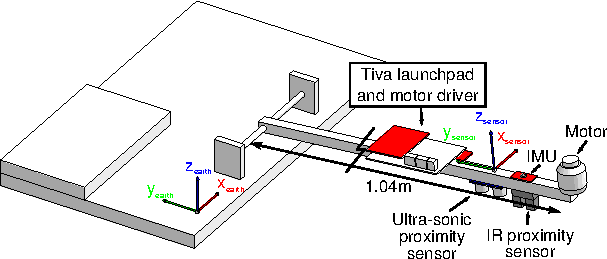
\includegraphics[width=\columnwidth]{pictures/arbejds_tegning}
	\caption{View of the test setup showing earth and sensor reference frames, placement of the IMU containing the 
	accelerometer and rate gyroscope as well as the placement of the Tiva Launchpad. The arm length is 1.04m.}
	\label{fig:labsetup}
\end{figure}
\begin{figure}
	\centering
	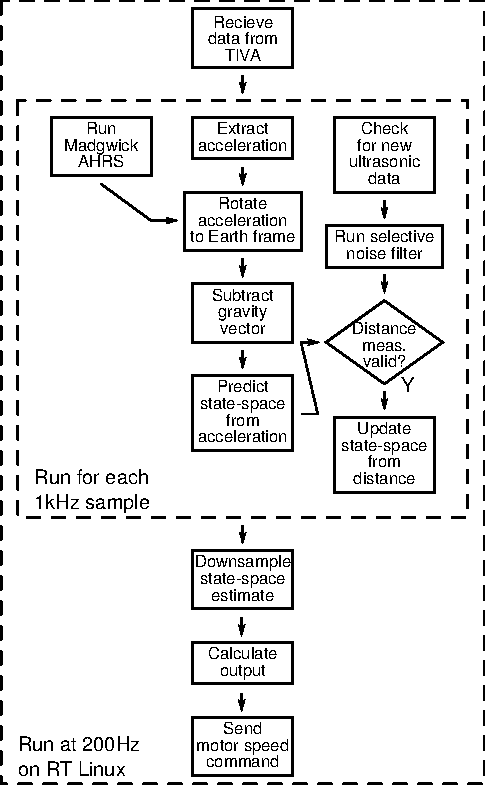
\includegraphics[width=\columnwidth]{pictures/process}
	\caption{View of main control loop.}
	\label{fig:labsetup}
\end{figure}

\subsection{Communications subsystem}\label{sec:comms}
The Tiva Launcpad recieves measurements from the accelerometer, rate gyroscope and ultrasound sensor. The accelerometer and 
rate gyroscope is sampled at 1kHz, while the ultrasound sensor has a varying sample rate that depends on the distance to the nearest
object.
It is advantageous to sample at 1kHz because the rotor movement creates
vibration mainly at \(\sim\)70Hz, but also at the second and third harmonics thereof.
Hermansen should have been able to see this as he sampled at 200Hz, resulting in folding of the second and third
harmonic.

The measurement data is transformed into a packet where the leading bit of every byte contains a synchronization bit. When
the bit is set it signifies the start of a packet. These packets are then sent to the desktop machine at 1kHz. When the ultrasound 
sensor is not ready with a new measurement, zeroes are transmitted as its data
instead.
The packets are received on the desktop machine, which is running a control loop at 200Hz. Here the packets are unpacked to their
original form and corrupted packets are attempted detected and thrown away.
\subsection{Localisation}\label{sec:localisation}
Our localisation algorithm is a three step process. First the accelerometer and
rate gyroscope measurements are used to determine the orientation of the arm.
This is done using the Madgwick AHRS algorithm\cite{Madgwick2011}.
It is necessary to know the orientation of the arm before
the acceleration can be calculated because the acceleration measured by the tri-axis MEMs accelerometer is relative to the 
accelerometer frame. Additionally, gravity results in an offset in the accelerometer measurements that has constant magnitude, but
orientation varying with the orientation of the accelerometer. The acceleration
is then rotated into earth frame, the gravity vector is subtracted and the
vertical acceleration is isolated since we only care about the height of the arm.
This is then used as the control input to a static multi rate kalman filter\cite{Welch2006}.

Because the filter is static we
only predict the new state 
\begin{equation*}
	\hat{\mathbf{x}}_{k\vert k-1} = \mathbf{F}\hat{\mathbf{x}}_{k-1\vert k-1} + \mathbf{B}a
\end{equation*}
Compute the measurement error 
\begin{equation*}
	y = z_k - \mathbf{H}\hat{\mathbf{x}}_{k\vert k-1} 
\end{equation*}
And update the state
\begin{equation*}
	\hat{\mathbf{x}}_{k\vert k} = \hat{\mathbf{x}}_{k\vert k-1} + \mathbf{K} y
\end{equation*}

The kalman filter executes a predict step for every measurement coming from the accelerometer at 1kHz and an update step as soon 
as a measurement is received from the distance sensor, be it ultrasound or infrared. When using the IR distance 
sensor a measurement is always ready, however it is only updated at
\(\sim\)20Hz. With the ultrasound sensor however, a measurement is only valid in the same sample it is recorded. The ultrasound sensor is also afflicted by intermittent noise that results in false readings,
typically far away from previous values. We employ a gating filter that culls out measurements too far from a moving average.

Let \(x_k\) be the current measurement sample, \(w\) the number of measurements taken into the moving average and \(Z\) the threshold value.
A measurement is then accepted if 
\begin{equation*}
	Z >\frac{1}{w} \left\lvert \sum_{i=k-w}^{k}x_i \right\rvert
\end{equation*}
This improves stability greatly as we rely somewhat heavily on the low frequency distance measurements in the kalman filter.
\begin{figure*}
	\centering
	\subfloat[][]{\newlength\figureheight
		\newlength\figurewidth
		\setlength\figureheight{4cm}
		\setlength\figurewidth{7cm}
		% This file was created by matlab2tikz v0.4.7 running on MATLAB 8.0.
% Copyright (c) 2008--2014, Nico Schlömer <nico.schloemer@gmail.com>
% All rights reserved.
% Minimal pgfplots version: 1.3
% 
% The latest updates can be retrieved from
%   http://www.mathworks.com/matlabcentral/fileexchange/22022-matlab2tikz
% where you can also make suggestions and rate matlab2tikz.
% 
\begin{tikzpicture}

\begin{axis}[%
width=\figurewidth,
height=\figureheight,
scale only axis,
xmin=0,
xmax=100,
xlabel={time [s]},
ymin=-0.1,
ymax=0.25,
ylabel={distance [m] / angle [rad]},
axis x line*=bottom,
axis y line*=left,
legend style={at={(0.03,0.97)},anchor=north west,draw=black,fill=white,legend cell align=left}
]
\addplot [color=black!50!green,solid,line width=0.1pt]
  table[row sep=crcr]{0	0\\
0.0500027536072255	0\\
0.100005507214451	0\\
0.150008260821676	0\\
0.200011014428902	0\\
0.250013768036127	0\\
0.300016521643353	0\\
0.350019275250578	0\\
0.400022028857804	0\\
0.450024782465029	0\\
0.500027536072255	0\\
0.55003028967948	0\\
0.600033043286706	0\\
0.650035796893931	0\\
0.700038550501157	0\\
0.750041304108382	0\\
0.800044057715607	0\\
0.850046811322833	0\\
0.900049564930058	0\\
0.950052318537284	0\\
1.00005507214451	0\\
1.05005782575173	0\\
1.10006057935896	0\\
1.15006333296619	0\\
1.20006608657341	0\\
1.25006884018064	0\\
1.30007159378786	0\\
1.35007434739509	0\\
1.40007710100231	0\\
1.45007985460954	0\\
1.50008260821676	0\\
1.55008536182399	0\\
1.60008811543122	0\\
1.65009086903844	0\\
1.70009362264567	0\\
1.75009637625289	0\\
1.80009912986012	0\\
1.85010188346734	0\\
1.90010463707457	0\\
1.95010739068179	0\\
2.00011014428902	0\\
2.05011289789624	0\\
2.10011565150347	0\\
2.15011840511069	0\\
2.20012115871792	0\\
2.25012391232515	0\\
2.30012666593237	0\\
2.3501294195396	0\\
2.40013217314682	0\\
2.45013492675405	0\\
2.50013768036127	0\\
2.5501404339685	0\\
2.60014318757572	0\\
2.65014594118295	0\\
2.70014869479018	0\\
2.7501514483974	0\\
2.80015420200463	0\\
2.85015695561185	0\\
2.90015970921908	0\\
2.9501624628263	0\\
3.00016521643353	0\\
3.05016797004075	0\\
3.10017072364798	0\\
3.1501734772552	0\\
3.20017623086243	0\\
3.25017898446966	0\\
3.30018173807688	0\\
3.35018449168411	0\\
3.40018724529133	0\\
3.45018999889856	0\\
3.50019275250578	0\\
3.55019550611301	0\\
3.60019825972023	0\\
3.65020101332746	0\\
3.70020376693468	0\\
3.75020652054191	0\\
3.80020927414914	0\\
3.85021202775636	0\\
3.90021478136359	0\\
3.95021753497081	0\\
4.00022028857804	0\\
4.05022304218526	0\\
4.10022579579249	0\\
4.15022854939971	0\\
4.20023130300694	0\\
4.25023405661416	0\\
4.30023681022139	0\\
4.35023956382862	0\\
4.40024231743584	0\\
4.45024507104307	0\\
4.50024782465029	0\\
4.55025057825752	0\\
4.60025333186474	0\\
4.65025608547197	0\\
4.70025883907919	0\\
4.75026159268642	0\\
4.80026434629364	0\\
4.85026709990087	0\\
4.9002698535081	0\\
4.95027260711532	0\\
5.00027536072255	0\\
5.05027811432977	0\\
5.100280867937	0\\
5.15028362154422	0\\
5.20028637515145	0\\
5.25028912875867	0\\
5.3002918823659	0\\
5.35029463597313	0\\
5.40029738958035	0\\
5.45030014318758	0\\
5.5003028967948	0\\
5.55030565040203	0\\
5.60030840400925	0\\
5.65031115761648	0\\
5.7003139112237	0\\
5.75031666483093	0\\
5.80031941843815	0\\
5.85032217204538	0\\
5.90032492565261	0\\
5.95032767925983	0\\
6.00033043286706	0\\
6.05033318647428	0\\
6.10033594008151	0\\
6.15033869368873	0\\
6.20034144729596	0\\
6.25034420090318	0\\
6.30034695451041	0\\
6.35034970811763	0\\
6.40035246172486	0\\
6.45035521533209	0\\
6.50035796893931	0\\
6.55036072254654	0\\
6.60036347615376	0\\
6.65036622976099	0\\
6.70036898336821	0\\
6.75037173697544	0\\
6.80037449058266	0\\
6.85037724418989	0\\
6.90037999779711	0\\
6.95038275140434	0\\
7.00038550501157	0\\
7.05038825861879	0\\
7.10039101222602	0\\
7.15039376583324	0\\
7.20039651944047	0\\
7.25039927304769	0\\
7.30040202665492	0\\
7.35040478026214	0\\
7.40040753386937	0\\
7.45041028747659	0\\
7.50041304108382	0\\
7.55041579469105	0\\
7.60041854829827	0\\
7.6504213019055	0\\
7.70042405551272	0\\
7.75042680911995	0\\
7.80042956272717	0\\
7.8504323163344	0\\
7.90043506994162	0\\
7.95043782354885	0\\
8.00044057715608	0\\
8.0504433307633	0\\
8.10044608437052	0\\
8.15044883797775	0\\
8.20045159158498	0\\
8.2504543451922	0\\
8.30045709879943	0\\
8.35045985240665	0\\
8.40046260601388	0\\
8.4504653596211	0\\
8.50046811322833	0\\
8.55047086683556	0\\
8.60047362044278	0\\
8.65047637405001	0\\
8.70047912765723	0\\
8.75048188126446	0\\
8.80048463487168	0\\
8.85048738847891	0\\
8.90049014208613	0\\
8.95049289569336	0\\
9.00049564930058	0\\
9.05049840290781	0\\
9.10050115651504	0\\
9.15050391012226	0\\
9.20050666372949	0\\
9.25050941733671	0\\
9.30051217094394	0\\
9.35051492455116	0\\
9.40051767815839	0\\
9.45052043176561	0\\
9.50052318537284	0\\
9.55052593898006	0\\
9.60052869258729	0\\
9.65053144619452	0\\
9.70053419980174	0\\
9.75053695340897	0\\
9.80053970701619	0\\
9.85054246062342	0\\
9.90054521423064	0\\
9.95054796783787	0\\
10.0005507214451	0\\
10.0505534750523	0\\
10.1005562286595	0\\
10.1505589822668	0\\
10.200561735874	0\\
10.2505644894812	0\\
10.3005672430884	0\\
10.3505699966957	0\\
10.4005727503029	0\\
10.4505755039101	0\\
10.5005782575173	0\\
10.5505810111246	0\\
10.6005837647318	0\\
10.650586518339	0\\
10.7005892719463	0\\
10.7505920255535	0\\
10.8005947791607	0\\
10.8505975327679	0\\
10.9006002863752	0\\
10.9506030399824	0\\
11.0006057935896	0\\
11.0506085471968	0\\
11.1006113008041	0\\
11.1506140544113	0\\
11.2006168080185	0\\
11.2506195616257	0\\
11.300622315233	0\\
11.3506250688402	0\\
11.4006278224474	0\\
11.4506305760546	0\\
11.5006333296619	0\\
11.5506360832691	0\\
11.6006388368763	0\\
11.6506415904835	0\\
11.7006443440908	0\\
11.750647097698	0\\
11.8006498513052	0\\
11.8506526049124	0\\
11.9006553585197	0\\
11.9506581121269	0\\
12.0006608657341	0\\
12.0506636193413	0\\
12.1006663729486	0\\
12.1506691265558	0\\
12.200671880163	0\\
12.2506746337702	0\\
12.3006773873775	0\\
12.3506801409847	0\\
12.4006828945919	0\\
12.4506856481991	0\\
12.5006884018064	0\\
12.5506911554136	0\\
12.6006939090208	0\\
12.650696662628	0\\
12.7006994162353	0\\
12.7507021698425	0\\
12.8007049234497	0\\
12.8507076770569	0\\
12.9007104306642	0\\
12.9507131842714	0\\
13.0007159378786	0\\
13.0507186914858	0\\
13.1007214450931	0\\
13.1507241987003	0\\
13.2007269523075	0\\
13.2507297059147	0\\
13.300732459522	0\\
13.3507352131292	0\\
13.4007379667364	0\\
13.4507407203437	0\\
13.5007434739509	0\\
13.5507462275581	0\\
13.6007489811653	0\\
13.6507517347726	0\\
13.7007544883798	0\\
13.750757241987	0\\
13.8007599955942	0\\
13.8507627492015	0\\
13.9007655028087	0\\
13.9507682564159	0\\
14.0007710100231	0\\
14.0507737636304	0\\
14.1007765172376	0\\
14.1507792708448	0\\
14.200782024452	0\\
14.2507847780593	0\\
14.3007875316665	0\\
14.3507902852737	0\\
14.4007930388809	0\\
14.4507957924882	0\\
14.5007985460954	0\\
14.5508012997026	0\\
14.6008040533098	0\\
14.6508068069171	0\\
14.7008095605243	0\\
14.7508123141315	0\\
14.8008150677387	0\\
14.850817821346	0\\
14.9008205749532	0\\
14.9508233285604	0\\
15.0008260821676	0\\
15.0508288357749	0\\
15.1008315893821	0\\
15.1508343429893	0\\
15.2008370965965	0\\
15.2508398502038	0\\
15.300842603811	0\\
15.3508453574182	0\\
15.4008481110254	0\\
15.4508508646327	0\\
15.5008536182399	0\\
15.5508563718471	0\\
15.6008591254543	0\\
15.6508618790616	0\\
15.7008646326688	0\\
15.750867386276	0\\
15.8008701398832	0\\
15.8508728934905	0\\
15.9008756470977	0\\
15.9508784007049	0\\
16.0008811543122	0\\
16.0508839079194	0\\
16.1008866615266	0\\
16.1508894151338	0\\
16.200892168741	0\\
16.2508949223483	0\\
16.3008976759555	0\\
16.3509004295627	0\\
16.40090318317	0\\
16.4509059367772	0\\
16.5009086903844	0\\
16.5509114439916	0\\
16.6009141975989	0\\
16.6509169512061	0\\
16.7009197048133	0\\
16.7509224584205	0\\
16.8009252120278	0\\
16.850927965635	0\\
16.9009307192422	0\\
16.9509334728494	0\\
17.0009362264567	0\\
17.0509389800639	0\\
17.1009417336711	0\\
17.1509444872783	0\\
17.2009472408856	0\\
17.2509499944928	0\\
17.3009527481	0\\
17.3509555017072	0\\
17.4009582553145	0\\
17.4509610089217	0\\
17.5009637625289	0\\
17.5509665161361	0\\
17.6009692697434	0\\
17.6509720233506	0\\
17.7009747769578	0\\
17.750977530565	0\\
17.8009802841723	0\\
17.8509830377795	0\\
17.9009857913867	0\\
17.9509885449939	0\\
18.0009912986012	0\\
18.0509940522084	0\\
18.1009968058156	0\\
18.1509995594228	0\\
18.2010023130301	0\\
18.2510050666373	0\\
18.3010078202445	0\\
18.3510105738517	0\\
18.401013327459	0\\
18.4510160810662	0\\
18.5010188346734	0\\
18.5510215882806	0\\
18.6010243418879	0\\
18.6510270954951	0\\
18.7010298491023	0\\
18.7510326027096	0\\
18.8010353563168	0\\
18.851038109924	0\\
18.9010408635312	0\\
18.9510436171384	0\\
19.0010463707457	0\\
19.0510491243529	0\\
19.1010518779601	0\\
19.1510546315674	0\\
19.2010573851746	0\\
19.2510601387818	0\\
19.301062892389	0\\
19.3510656459963	0\\
19.4010683996035	0\\
19.4510711532107	0\\
19.5010739068179	0\\
19.5510766604252	0\\
19.6010794140324	0\\
19.6510821676396	0\\
19.7010849212468	0\\
19.7510876748541	0\\
19.8010904284613	0\\
19.8510931820685	0\\
19.9010959356757	0\\
19.951098689283	0\\
20.0011014428902	0\\
20.0511041964974	0\\
20.1011069501046	0\\
20.1511097037119	0\\
20.2011124573191	0\\
20.2511152109263	0\\
20.3011179645335	0\\
20.3511207181408	0\\
20.401123471748	0\\
20.4511262253552	0\\
20.5011289789624	0\\
20.5511317325697	0\\
20.6011344861769	0\\
20.6511372397841	0\\
20.7011399933913	0\\
20.7511427469986	0\\
20.8011455006058	0\\
20.851148254213	0\\
20.9011510078202	0\\
20.9511537614275	0\\
21.0011565150347	0\\
21.0511592686419	0\\
21.1011620222491	0\\
21.1511647758564	0\\
21.2011675294636	0\\
21.2511702830708	0\\
21.301173036678	0\\
21.3511757902853	0\\
21.4011785438925	0\\
21.4511812974997	0\\
21.501184051107	0\\
21.5511868047142	0\\
21.6011895583214	0\\
21.6511923119286	0\\
21.7011950655359	0\\
21.7511978191431	0\\
21.8012005727503	0\\
21.8512033263575	0\\
21.9012060799648	0\\
21.951208833572	0\\
22.0012115871792	0\\
22.0512143407864	0\\
22.1012170943937	0\\
22.1512198480009	0\\
22.2012226016081	0\\
22.2512253552153	0\\
22.3012281088226	0\\
22.3512308624298	0\\
22.401233616037	0\\
22.4512363696442	0\\
22.5012391232515	0\\
22.5512418768587	0\\
22.6012446304659	0\\
22.6512473840731	0\\
22.7012501376804	0\\
22.7512528912876	0\\
22.8012556448948	0\\
22.851258398502	0\\
22.9012611521093	0\\
22.9512639057165	0\\
23.0012666593237	0\\
23.0512694129309	0\\
23.1012721665382	0\\
23.1512749201454	0\\
23.2012776737526	0\\
23.2512804273598	0\\
23.3012831809671	0\\
23.3512859345743	0\\
23.4012886881815	0\\
23.4512914417887	0\\
23.501294195396	0\\
23.5512969490032	0\\
23.6012997026104	0\\
23.6513024562176	0\\
23.7013052098249	0\\
23.7513079634321	0\\
23.8013107170393	0\\
23.8513134706465	0\\
23.9013162242538	0\\
23.951318977861	0\\
24.0013217314682	0\\
24.0513244850755	0\\
24.1013272386827	0\\
24.1513299922899	0\\
24.2013327458971	0\\
24.2513354995044	0\\
24.3013382531116	0\\
24.3513410067188	0\\
24.401343760326	0\\
24.4513465139333	0\\
24.5013492675405	0\\
24.5513520211477	0\\
24.6013547747549	0\\
24.6513575283622	0\\
24.7013602819694	0\\
24.7513630355766	0\\
24.8013657891838	0\\
24.8513685427911	0\\
24.9013712963983	0\\
24.9513740500055	0\\
25.0013768036127	0\\
25.05137955722	0\\
25.1013823108272	0\\
25.1513850644344	0\\
25.2013878180416	0\\
25.2513905716489	0\\
25.3013933252561	0\\
25.3513960788633	0\\
25.4013988324705	0\\
25.4514015860778	0\\
25.501404339685	0\\
25.5514070932922	0\\
25.6014098468994	0\\
25.6514126005067	0\\
25.7014153541139	0\\
25.7514181077211	0\\
25.8014208613283	0\\
25.8514236149356	0\\
25.9014263685428	0\\
25.95142912215	0\\
26.0014318757572	0\\
26.0514346293645	0\\
26.1014373829717	0\\
26.1514401365789	0\\
26.2014428901861	0\\
26.2514456437934	0\\
26.3014483974006	0\\
26.3514511510078	0\\
26.401453904615	0\\
26.4514566582223	0\\
26.5014594118295	0\\
26.5514621654367	0\\
26.6014649190439	0\\
26.6514676726512	0\\
26.7014704262584	0\\
26.7514731798656	0\\
26.8014759334729	0\\
26.8514786870801	0\\
26.9014814406873	0\\
26.9514841942945	0\\
27.0014869479018	0\\
27.051489701509	0\\
27.1014924551162	0\\
27.1514952087234	0\\
27.2014979623307	0\\
27.2515007159379	0\\
27.3015034695451	0\\
27.3515062231523	0\\
27.4015089767596	0\\
27.4515117303668	0\\
27.501514483974	0\\
27.5515172375812	0\\
27.6015199911885	0\\
27.6515227447957	0\\
27.7015254984029	0\\
27.7515282520101	0\\
27.8015310056174	0\\
27.8515337592246	0\\
27.9015365128318	0\\
27.951539266439	0\\
28.0015420200463	0\\
28.0515447736535	0\\
28.1015475272607	0\\
28.1515502808679	0\\
28.2015530344752	0\\
28.2515557880824	0\\
28.3015585416896	0\\
28.3515612952968	0\\
28.4015640489041	0\\
28.4515668025113	0\\
28.5015695561185	0\\
28.5515723097257	0\\
28.601575063333	0\\
28.6515778169402	0\\
28.7015805705474	0\\
28.7515833241546	0\\
28.8015860777619	0\\
28.8515888313691	0\\
28.9015915849763	0\\
28.9515943385835	0\\
29.0015970921908	0\\
29.051599845798	0\\
29.1016025994052	0\\
29.1516053530124	0\\
29.2016081066197	0\\
29.2516108602269	0\\
29.3016136138341	0\\
29.3516163674413	0\\
29.4016191210486	0\\
29.4516218746558	0\\
29.501624628263	0\\
29.5516273818702	0\\
29.6016301354775	0\\
29.6516328890847	0\\
29.7016356426919	0\\
29.7516383962992	0\\
29.8016411499064	0\\
29.8516439035136	0\\
29.9016466571208	0\\
29.9516494107281	0\\
30.0016521643353	0\\
30.0516549179425	0\\
30.1016576715497	0\\
30.151660425157	0\\
30.2016631787642	0\\
30.2516659323714	0\\
30.3016686859786	0\\
30.3516714395859	0\\
30.4016741931931	0\\
30.4516769468003	0\\
30.5016797004075	0\\
30.5516824540148	0\\
30.601685207622	0\\
30.6516879612292	0\\
30.7016907148364	0\\
30.7516934684437	0\\
30.8016962220509	0\\
30.8516989756581	0\\
30.9017017292653	0\\
30.9517044828726	0\\
31.0017072364798	0\\
31.051709990087	0\\
31.1017127436942	0\\
31.1517154973015	0\\
31.2017182509087	0\\
31.2517210045159	0\\
31.3017237581231	0\\
31.3517265117304	0\\
31.4017292653376	0\\
31.4517320189448	0\\
31.501734772552	0\\
31.5517375261593	0\\
31.6017402797665	0\\
31.6517430333737	0\\
31.7017457869809	0\\
31.7517485405882	0\\
31.8017512941954	0\\
31.8517540478026	0\\
31.9017568014098	0\\
31.9517595550171	0\\
32.0017623086243	0\\
32.0517650622315	0\\
32.1017678158387	0\\
32.151770569446	0\\
32.2017733230532	0\\
32.2517760766604	0\\
32.3017788302677	0\\
32.3517815838749	0\\
32.4017843374821	0\\
32.4517870910893	0\\
32.5017898446966	0\\
32.5517925983038	0\\
32.601795351911	0\\
32.6517981055182	0\\
32.7018008591255	0\\
32.7518036127327	0\\
32.8018063663399	0\\
32.8518091199471	0\\
32.9018118735544	0\\
32.9518146271616	0\\
33.0018173807688	0\\
33.051820134376	0\\
33.1018228879833	0\\
33.1518256415905	0\\
33.2018283951977	0\\
33.2518311488049	0\\
33.3018339024122	0\\
33.3518366560194	0\\
33.4018394096266	0\\
33.4518421632338	0\\
33.5018449168411	0\\
33.5518476704483	0\\
33.6018504240555	0\\
33.6518531776627	0\\
33.70185593127	0\\
33.7518586848772	0\\
33.8018614384844	0\\
33.8518641920916	0\\
33.9018669456989	0\\
33.9518696993061	0\\
34.0018724529133	0\\
34.0518752065205	0\\
34.1018779601278	0\\
34.151880713735	0\\
34.2018834673422	0\\
34.2518862209494	0\\
34.3018889745567	0\\
34.3518917281639	0\\
34.4018944817711	0\\
34.4518972353783	0\\
34.5018999889856	0\\
34.5519027425928	0\\
34.6019054962	0\\
34.6519082498072	0\\
34.7019110034145	0\\
34.7519137570217	0\\
34.8019165106289	0\\
34.8519192642362	0\\
34.9019220178434	0\\
34.9519247714506	0\\
35.0019275250578	0\\
35.0519302786651	0\\
35.1019330322723	0\\
35.1519357858795	0\\
35.2019385394867	0\\
35.251941293094	0\\
35.3019440467012	0\\
35.3519468003084	0\\
35.4019495539156	0\\
35.4519523075229	0\\
35.5019550611301	0\\
35.5519578147373	0\\
35.6019605683445	0\\
35.6519633219518	0\\
35.701966075559	0\\
35.7519688291662	0\\
35.8019715827734	0\\
35.8519743363807	0\\
35.9019770899879	0\\
35.9519798435951	0\\
36.0019825972023	0\\
36.0519853508096	0\\
36.1019881044168	0\\
36.151990858024	0\\
36.2019936116312	0\\
36.2519963652385	0\\
36.3019991188457	0\\
36.3520018724529	0\\
36.4020046260601	0\\
36.4520073796674	0\\
36.5020101332746	0\\
36.5520128868818	0\\
36.602015640489	0\\
36.6520183940963	0\\
36.7020211477035	0\\
36.7520239013107	0\\
36.8020266549179	0\\
36.8520294085252	0\\
36.9020321621324	0\\
36.9520349157396	0\\
37.0020376693468	0\\
37.0520404229541	0\\
37.1020431765613	0\\
37.1520459301685	0\\
37.2020486837758	0\\
37.252051437383	0\\
37.3020541909902	0\\
37.3520569445974	0\\
37.4020596982046	0\\
37.4520624518119	0\\
37.5020652054191	0\\
37.5520679590263	0\\
37.6020707126335	0\\
37.6520734662408	0\\
37.702076219848	0\\
37.7520789734552	0\\
37.8020817270625	0\\
37.8520844806697	0\\
37.9020872342769	0\\
37.9520899878841	0\\
38.0020927414914	0\\
38.0520954950986	0\\
38.1020982487058	0\\
38.152101002313	0\\
38.2021037559203	0\\
38.2521065095275	0\\
38.3021092631347	0\\
38.3521120167419	0\\
38.4021147703492	0\\
38.4521175239564	0\\
38.5021202775636	0\\
38.5521230311708	0\\
38.6021257847781	0\\
38.6521285383853	0\\
38.7021312919925	0\\
38.7521340455997	0\\
38.802136799207	0\\
38.8521395528142	0\\
38.9021423064214	0\\
38.9521450600286	0\\
39.0021478136359	0\\
39.0521505672431	0\\
39.1021533208503	0\\
39.1521560744575	0\\
39.2021588280648	0\\
39.252161581672	0\\
39.3021643352792	0\\
39.3521670888864	0\\
39.4021698424937	0\\
39.4521725961009	0\\
39.5021753497081	0\\
39.5521781033153	0\\
39.6021808569226	0\\
39.6521836105298	0\\
39.702186364137	0\\
39.7521891177442	0\\
39.8021918713515	0\\
39.8521946249587	0\\
39.9021973785659	0\\
39.9522001321731	0\\
40.0022028857804	0\\
40.0522056393876	0\\
40.1022083929948	0\\
40.152211146602	0\\
40.2022139002093	0\\
40.2522166538165	0\\
40.3022194074237	0\\
40.352222161031	0\\
40.4022249146382	0\\
40.4522276682454	0\\
40.5022304218526	0\\
40.5522331754599	0\\
40.6022359290671	0\\
40.6522386826743	0\\
40.7022414362815	0\\
40.7522441898888	0\\
40.802246943496	0\\
40.8522496971032	0\\
40.9022524507104	0\\
40.9522552043177	0\\
41.0022579579249	0\\
41.0522607115321	0\\
41.1022634651393	0\\
41.1522662187466	0\\
41.2022689723538	0\\
41.252271725961	0\\
41.3022744795682	0\\
41.3522772331755	0\\
41.4022799867827	0\\
41.4522827403899	0\\
41.5022854939971	0\\
41.5522882476044	0\\
41.6022910012116	0\\
41.6522937548188	0\\
41.702296508426	0\\
41.7522992620333	0\\
41.8023020156405	0\\
41.8523047692477	0\\
41.9023075228549	0\\
41.9523102764622	0\\
42.0023130300694	0\\
42.0523157836766	0\\
42.1023185372838	0\\
42.1523212908911	0\\
42.2023240444983	0\\
42.2523267981055	0\\
42.3023295517127	0\\
42.35233230532	0\\
42.4023350589272	0\\
42.4523378125344	0\\
42.5023405661416	0\\
42.5523433197489	0\\
42.6023460733561	0\\
42.6523488269633	0\\
42.7023515805706	0\\
42.7523543341778	0\\
42.802357087785	0\\
42.8523598413922	0\\
42.9023625949994	0\\
42.9523653486067	0\\
43.0023681022139	0\\
43.0523708558211	0\\
43.1023736094284	0\\
43.1523763630356	0\\
43.2023791166428	0\\
43.25238187025	0\\
43.3023846238573	0\\
43.3523873774645	0\\
43.4023901310717	0\\
43.4523928846789	0\\
43.5023956382862	0\\
43.5523983918934	0\\
43.6024011455006	0\\
43.6524038991078	0\\
43.7024066527151	0\\
43.7524094063223	0\\
43.8024121599295	0\\
43.8524149135367	0\\
43.902417667144	0\\
43.9524204207512	0\\
44.0024231743584	0\\
44.0524259279656	0\\
44.1024286815729	0\\
44.1524314351801	0\\
44.2024341887873	0\\
44.2524369423945	0\\
44.3024396960018	0\\
44.352442449609	0\\
44.4024452032162	0\\
44.4524479568234	0\\
44.5024507104307	0\\
44.5524534640379	0\\
44.6024562176451	0\\
44.6524589712523	0\\
44.7024617248596	0\\
44.7524644784668	0\\
44.802467232074	0\\
44.8524699856812	0\\
44.9024727392885	0\\
44.9524754928957	0\\
45.0024782465029	0\\
45.0524810001101	0\\
45.1024837537174	0\\
45.1524865073246	0\\
45.2024892609318	0\\
45.252492014539	0\\
45.3024947681463	0\\
45.3524975217535	0\\
45.4025002753607	0\\
45.452503028968	0\\
45.5025057825752	0\\
45.5525085361824	0\\
45.6025112897896	0\\
45.6525140433968	0\\
45.7025167970041	0\\
45.7525195506113	0\\
45.8025223042185	0\\
45.8525250578258	0\\
45.902527811433	0\\
45.9525305650402	0\\
46.0025333186474	0\\
46.0525360722547	0\\
46.1025388258619	0\\
46.1525415794691	0\\
46.2025443330763	0\\
46.2525470866836	0\\
46.3025498402908	0\\
46.352552593898	0\\
46.4025553475052	0\\
46.4525581011125	0\\
46.5025608547197	0\\
46.5525636083269	0\\
46.6025663619341	0\\
46.6525691155414	0\\
46.7025718691486	0\\
46.7525746227558	0\\
46.802577376363	0\\
46.8525801299703	0\\
46.9025828835775	0\\
46.9525856371847	0\\
47.0025883907919	0\\
47.0525911443992	0\\
47.1025938980064	0\\
47.1525966516136	0\\
47.2025994052208	0\\
47.2526021588281	0\\
47.3026049124353	0\\
47.3526076660425	0\\
47.4026104196497	0\\
47.452613173257	0\\
47.5026159268642	0\\
47.5526186804714	0\\
47.6026214340786	0\\
47.6526241876859	0\\
47.7026269412931	0\\
47.7526296949003	0\\
47.8026324485076	0\\
47.8526352021148	0\\
47.902637955722	0\\
47.9526407093292	0\\
48.0026434629364	0\\
48.0526462165437	0\\
48.1026489701509	0\\
48.1526517237581	0\\
48.2026544773654	0\\
48.2526572309726	0\\
48.3026599845798	0\\
48.352662738187	0\\
48.4026654917943	0\\
48.4526682454015	0\\
48.5026709990087	0\\
48.5526737526159	0\\
48.6026765062232	0\\
48.6526792598304	0\\
48.7026820134376	0\\
48.7526847670448	0\\
48.8026875206521	0\\
48.8526902742593	0\\
48.9026930278665	0\\
48.9526957814737	0\\
49.002698535081	0\\
49.0527012886882	0\\
49.1027040422954	0\\
49.1527067959026	0\\
49.2027095495099	0\\
49.2527123031171	0\\
49.3027150567243	0\\
49.3527178103315	0\\
49.4027205639388	0\\
49.452723317546	0\\
49.5027260711532	0\\
49.5527288247604	0\\
49.6027315783677	0\\
49.6527343319749	0\\
49.7027370855821	0\\
49.7527398391893	0\\
49.8027425927966	0\\
49.8527453464038	0\\
49.902748100011	0\\
49.9527508536182	0\\
50.0027536072255	0\\
50.0527563608327	0\\
50.1027591144399	0\\
50.1527618680471	0\\
50.2027646216544	0\\
50.2527673752616	0\\
50.3027701288688	0\\
50.352772882476	0\\
50.4027756360833	0\\
50.4527783896905	0\\
50.5027811432977	0\\
50.5527838969049	0\\
50.6027866505122	0\\
50.6527894041194	0\\
50.7027921577266	0\\
50.7527949113339	0\\
50.8027976649411	0\\
50.8528004185483	0\\
50.9028031721555	0\\
50.9528059257628	0\\
51.00280867937	0\\
51.0528114329772	0\\
51.1028141865844	0\\
51.1528169401916	0\\
51.2028196937989	0\\
51.2528224474061	0\\
51.3028252010133	0\\
51.3528279546206	0\\
51.4028307082278	0\\
51.452833461835	0\\
51.5028362154422	0\\
51.5528389690495	0\\
51.6028417226567	0\\
51.6528444762639	0\\
51.7028472298711	0\\
51.7528499834784	0\\
51.8028527370856	0\\
51.8528554906928	0\\
51.9028582443	0\\
51.9528609979073	0\\
52.0028637515145	0\\
52.0528665051217	0\\
52.1028692587289	0\\
52.1528720123362	0\\
52.2028747659434	0\\
52.2528775195506	0\\
52.3028802731578	0\\
52.3528830267651	0\\
52.4028857803723	0\\
52.4528885339795	0\\
52.5028912875867	0\\
52.552894041194	0\\
52.6028967948012	0\\
52.6528995484084	0\\
52.7029023020156	0\\
52.7529050556229	0\\
52.8029078092301	0\\
52.8529105628373	0\\
52.9029133164445	0\\
52.9529160700518	0\\
53.002918823659	0\\
53.0529215772662	0\\
53.1029243308734	0\\
53.1529270844807	0\\
53.2029298380879	0\\
53.2529325916951	0\\
53.3029353453024	0\\
53.3529380989096	0\\
53.4029408525168	0\\
53.452943606124	0\\
53.5029463597312	0\\
53.5529491133385	0\\
53.6029518669457	0\\
53.6529546205529	0\\
53.7029573741602	0\\
53.7529601277674	0\\
53.8029628813746	0\\
53.8529656349818	0\\
53.9029683885891	0\\
53.9529711421963	0\\
54.0029738958035	0\\
54.0529766494107	0\\
54.102979403018	0\\
54.1529821566252	0\\
54.2029849102324	0\\
54.2529876638396	0\\
54.3029904174469	0\\
54.3529931710541	0\\
54.4029959246613	0\\
54.4529986782685	0\\
54.5030014318758	0\\
54.553004185483	0\\
54.6030069390902	0\\
54.6530096926974	0\\
54.7030124463047	0\\
54.7530151999119	0\\
54.8030179535191	0\\
54.8530207071263	0\\
54.9030234607336	0\\
54.9530262143408	0\\
55.003028967948	0\\
55.0530317215552	0\\
55.1030344751625	0\\
55.1530372287697	0\\
55.2030399823769	0\\
55.2530427359841	0\\
55.3030454895914	0\\
55.3530482431986	0\\
55.4030509968058	0\\
55.453053750413	0\\
55.5030565040203	0\\
55.5530592576275	0\\
55.6030620112347	0\\
55.6530647648419	0\\
55.7030675184492	0\\
55.7530702720564	0\\
55.8030730256636	0\\
55.8530757792708	0\\
55.9030785328781	0\\
55.9530812864853	0\\
56.0030840400925	0\\
56.0530867936997	0\\
56.103089547307	0\\
56.1530923009142	0\\
56.2030950545214	0\\
56.2530978081287	0\\
56.3031005617359	0\\
56.3531033153431	0\\
56.4031060689503	0\\
56.4531088225576	0\\
56.5031115761648	0\\
56.553114329772	0\\
56.6031170833792	0\\
56.6531198369864	0\\
56.7031225905937	0\\
56.7531253442009	0\\
56.8031280978081	0\\
56.8531308514154	0\\
56.9031336050226	0\\
56.9531363586298	0\\
57.003139112237	0\\
57.0531418658443	0\\
57.1031446194515	0\\
57.1531473730587	0\\
57.2031501266659	0\\
57.2531528802732	0\\
57.3031556338804	0\\
57.3531583874876	0\\
57.4031611410948	0\\
57.4531638947021	0\\
57.5031666483093	0\\
57.5531694019165	0\\
57.6031721555237	0\\
57.653174909131	0\\
57.7031776627382	0\\
57.7531804163454	0\\
57.8031831699526	0\\
57.8531859235599	0\\
57.9031886771671	0\\
57.9531914307743	0\\
58.0031941843815	0\\
58.0531969379888	0\\
58.103199691596	0\\
58.1532024452032	0\\
58.2032051988104	0\\
58.2532079524177	0\\
58.3032107060249	0\\
58.3532134596321	0\\
58.4032162132393	0\\
58.4532189668466	0\\
58.5032217204538	0\\
58.553224474061	0\\
58.6032272276682	0\\
58.6532299812755	0\\
58.7032327348827	0\\
58.7532354884899	0\\
58.8032382420971	0\\
58.8532409957044	0\\
58.9032437493116	0\\
58.9532465029188	0\\
59.003249256526	0\\
59.0532520101333	0\\
59.1032547637405	0\\
59.1532575173477	0\\
59.203260270955	0\\
59.2532630245622	0\\
59.3032657781694	0\\
59.3532685317766	0\\
59.4032712853839	0\\
59.4532740389911	0\\
59.5032767925983	0\\
59.5532795462055	0\\
59.6032822998127	0\\
59.65328505342	0\\
59.7032878070272	0\\
59.7532905606344	0\\
59.8032933142417	0\\
59.8532960678489	0\\
59.9032988214561	0\\
59.9533015750633	0\\
60.0033043286706	0\\
60.0533070822778	0\\
60.103309835885	0\\
60.1533125894922	0\\
60.2033153430995	0\\
60.2533180967067	0\\
60.3033208503139	0\\
60.3533236039211	0\\
60.4033263575284	0\\
60.4533291111356	0\\
60.5033318647428	0\\
60.55333461835	0\\
60.6033373719573	0\\
60.6533401255645	0\\
60.7033428791717	0\\
60.7533456327789	0\\
60.8033483863862	0\\
60.8533511399934	0\\
60.9033538936006	0\\
60.9533566472078	0\\
61.0033594008151	0\\
61.0533621544223	0\\
61.0733632558652	0.174528\\
61.1233660094724	0.174528\\
61.1733687630796	0.174528\\
61.2233715166869	0.174528\\
61.2733742702941	0.174528\\
61.3233770239013	0.174528\\
61.3733797775085	0.174528\\
61.4233825311158	0.174528\\
61.473385284723	0.174528\\
61.5233880383302	0.174528\\
61.5733907919374	0.174528\\
61.6233935455447	0.174528\\
61.6733962991519	0.174528\\
61.7233990527591	0.174528\\
61.7734018063663	0.174528\\
61.8234045599736	0.174528\\
61.8734073135808	0.174528\\
61.923410067188	0.174528\\
61.9734128207952	0.174528\\
62.0234155744025	0.174528\\
62.0734183280097	0.174528\\
62.1234210816169	0.174528\\
62.1734238352241	0.174528\\
62.2234265888314	0.174528\\
62.2734293424386	0.174528\\
62.3234320960458	0.174528\\
62.3734348496531	0.174528\\
62.4234376032603	0.174528\\
62.4734403568675	0.174528\\
62.5234431104747	0.174528\\
62.573445864082	0.174528\\
62.6234486176892	0.174528\\
62.6734513712964	0.174528\\
62.7234541249036	0.174528\\
62.7734568785108	0.174528\\
62.8234596321181	0.174528\\
62.8734623857253	0.174528\\
62.9234651393325	0.174528\\
62.9734678929398	0.174528\\
63.023470646547	0.174528\\
63.0734734001542	0.174528\\
63.1234761537614	0.174528\\
63.1734789073687	0.174528\\
63.2234816609759	0.174528\\
63.2734844145831	0.174528\\
63.3234871681903	0.174528\\
63.3734899217976	0.174528\\
63.4234926754048	0.174528\\
63.473495429012	0.174528\\
63.5234981826192	0.174528\\
63.5735009362265	0.174528\\
63.6235036898337	0.174528\\
63.6735064434409	0.174528\\
63.7235091970481	0.174528\\
63.7735119506554	0.174528\\
63.8235147042626	0.174528\\
63.8735174578698	0.174528\\
63.923520211477	0.174528\\
63.9735229650843	0.174528\\
64.0235257186915	0.174528\\
64.0735284722987	0.174528\\
64.1235312259059	0.174528\\
64.1735339795132	0.174528\\
64.2235367331204	0.174528\\
64.2735394867276	0.174528\\
64.3235422403348	0.174528\\
64.3735449939421	0.174528\\
64.4235477475493	0.174528\\
64.4735505011565	0.174528\\
64.5235532547637	0.174528\\
64.573556008371	0.174528\\
64.6235587619782	0.174528\\
64.6735615155854	0.174528\\
64.7235642691926	0.174528\\
64.7735670227999	0.174528\\
64.8235697764071	0.174528\\
64.8735725300143	0.174528\\
64.9235752836215	0.174528\\
64.9735780372288	0.174528\\
65.023580790836	0.174528\\
65.0735835444432	0.174528\\
65.1235862980505	0.174528\\
65.1735890516577	0.174528\\
65.2235918052649	0.174528\\
65.2735945588721	0.174528\\
65.3235973124794	0.174528\\
65.3736000660866	0.174528\\
65.4236028196938	0.174528\\
65.473605573301	0.174528\\
65.5236083269082	0.174528\\
65.5736110805155	0.174528\\
65.6236138341227	0.174528\\
65.6736165877299	0.174528\\
65.7236193413372	0.174528\\
65.7736220949444	0.174528\\
65.8236248485516	0.174528\\
65.8736276021588	0.174528\\
65.9236303557661	0.174528\\
65.9736331093733	0.174528\\
66.0236358629805	0.174528\\
66.0736386165877	0.174528\\
66.123641370195	0.174528\\
66.1736441238022	0.174528\\
66.2236468774094	0.174528\\
66.2736496310166	0.174528\\
66.3236523846239	0.174528\\
66.3736551382311	0.174528\\
66.4236578918383	0.174528\\
66.4736606454455	0.174528\\
66.5236633990528	0.174528\\
66.57366615266	0.174528\\
66.6236689062672	0.174528\\
66.6736716598744	0.174528\\
66.7236744134817	0.174528\\
66.7736771670889	0.174528\\
66.8236799206961	0.174528\\
66.8736826743033	0.174528\\
66.9236854279106	0.174528\\
66.9736881815178	0.174528\\
67.023690935125	0.174528\\
67.0736936887322	0.174528\\
67.1236964423395	0.174528\\
67.1736991959467	0.174528\\
67.2237019495539	0.174528\\
67.2737047031611	0.174528\\
67.3237074567684	0.174528\\
67.3737102103756	0.174528\\
67.4237129639828	0.174528\\
67.47371571759	0.174528\\
67.5237184711973	0.174528\\
67.5737212248045	0.174528\\
67.6237239784117	0.174528\\
67.6737267320189	0.174528\\
67.7237294856262	0.174528\\
67.7737322392334	0.174528\\
67.8237349928406	0.174528\\
67.8737377464478	0.174528\\
67.9237405000551	0.174528\\
67.9737432536623	0.174528\\
68.0237460072695	0.174528\\
68.0737487608768	0.174528\\
68.123751514484	0.174528\\
68.1737542680912	0.174528\\
68.2237570216984	0.174528\\
68.2737597753056	0.174528\\
68.3237625289129	0.174528\\
68.3737652825201	0.174528\\
68.4237680361273	0.174528\\
68.4737707897345	0.174528\\
68.5237735433418	0.174528\\
68.573776296949	0.174528\\
68.6237790505562	0.174528\\
68.6737818041635	0.174528\\
68.7237845577707	0.174528\\
68.7737873113779	0.174528\\
68.8237900649851	0.174528\\
68.8737928185924	0.174528\\
68.9237955721996	0.174528\\
68.9737983258068	0.174528\\
69.023801079414	0.174528\\
69.0738038330213	0.174528\\
69.1238065866285	0.174528\\
69.1738093402357	0.174528\\
69.2238120938429	0.174528\\
69.2738148474502	0.174528\\
69.3238176010574	0.174528\\
69.3738203546646	0.174528\\
69.4238231082718	0.174528\\
69.4738258618791	0.174528\\
69.5238286154863	0.174528\\
69.5738313690935	0.174528\\
69.6238341227007	0.174528\\
69.673836876308	0.174528\\
69.7238396299152	0.174528\\
69.7738423835224	0.174528\\
69.8238451371297	0.174528\\
69.8738478907369	0.174528\\
69.9238506443441	0.174528\\
69.9738533979513	0.174528\\
70.0238561515585	0.174528\\
70.0738589051658	0.174528\\
70.123861658773	0.174528\\
70.1738644123802	0.174528\\
70.2238671659874	0.174528\\
70.2738699195947	0.174528\\
70.3238726732019	0.174528\\
70.3738754268091	0.174528\\
70.4238781804164	0.174528\\
70.4738809340236	0.174528\\
70.5238836876308	0.174528\\
70.573886441238	0.174528\\
70.6238891948452	0.174528\\
70.6738919484525	0.174528\\
70.7238947020597	0.174528\\
70.7738974556669	0.174528\\
70.8239002092742	0.174528\\
70.8739029628814	0.174528\\
70.9239057164886	0.174528\\
70.9739084700958	0.174528\\
71.0239112237031	0.174528\\
71.0739139773103	0.174528\\
71.1239167309175	0.174528\\
71.1739194845247	0.174528\\
71.2239222381319	0.174528\\
71.2739249917392	0.174528\\
71.3239277453464	0.174528\\
71.3739304989536	0.174528\\
71.4239332525609	0.174528\\
71.4739360061681	0.174528\\
71.5239387597753	0.174528\\
71.5739415133825	0.174528\\
71.6239442669898	0.174528\\
71.673947020597	0.174528\\
71.7239497742042	0.174528\\
71.7739525278114	0.174528\\
71.8239552814187	0.174528\\
71.8739580350259	0.174528\\
71.9239607886331	0.174528\\
71.9739635422403	0.174528\\
72.0239662958476	0.174528\\
72.0739690494548	0.174528\\
72.123971803062	0.174528\\
72.1739745566692	0.174528\\
72.2239773102765	0.174528\\
72.2739800638837	0.174528\\
72.3239828174909	0.174528\\
72.3739855710981	0.174528\\
72.4239883247054	0.174528\\
72.4739910783126	0.174528\\
72.5239938319198	0.174528\\
72.573996585527	0.174528\\
72.6239993391343	0.174528\\
72.6740020927415	0.174528\\
72.7240048463487	0.174528\\
72.7740075999559	0.174528\\
72.8240103535632	0.174528\\
72.8740131071704	0.174528\\
72.9240158607776	0.174528\\
72.9740186143848	0.174528\\
73.0240213679921	0.174528\\
73.0740241215993	0.174528\\
73.1240268752065	0.174528\\
73.1740296288137	0.174528\\
73.224032382421	0.174528\\
73.2740351360282	0.174528\\
73.3240378896354	0.174528\\
73.3740406432427	0.174528\\
73.4240433968499	0.174528\\
73.4740461504571	0.174528\\
73.5240489040643	0.174528\\
73.5740516576716	0.174528\\
73.6240544112788	0.174528\\
73.674057164886	0.174528\\
73.7240599184932	0.174528\\
73.7740626721004	0.174528\\
73.8240654257077	0.174528\\
73.8740681793149	0.174528\\
73.9240709329221	0.174528\\
73.9740736865294	0.174528\\
74.0240764401366	0.174528\\
74.0740791937438	0.174528\\
74.124081947351	0.174528\\
74.1740847009583	0.174528\\
74.2240874545655	0.174528\\
74.2740902081727	0.174528\\
74.3240929617799	0.174528\\
74.3740957153872	0.174528\\
74.4240984689944	0.174528\\
74.4741012226016	0.174528\\
74.5241039762088	0.174528\\
74.5741067298161	0.174528\\
74.6241094834233	0.174528\\
74.6741122370305	0.174528\\
74.7241149906377	0.174528\\
74.774117744245	0.174528\\
74.8241204978522	0.174528\\
74.8741232514594	0.174528\\
74.9241260050666	0.174528\\
74.9741287586739	0.174528\\
75.0241315122811	0.174528\\
75.0741342658883	0.174528\\
75.1241370194955	0.174528\\
75.1741397731028	0.174528\\
75.22414252671	0.174528\\
75.2741452803172	0.174528\\
75.3241480339244	0.174528\\
75.3741507875317	0.174528\\
75.4241535411389	0.174528\\
75.4741562947461	0.174528\\
75.5241590483533	0.174528\\
75.5741618019606	0.174528\\
75.6241645555678	0.174528\\
75.674167309175	0.174528\\
75.7241700627823	0.174528\\
75.7741728163895	0.174528\\
75.8241755699967	0.174528\\
75.8741783236039	0.174528\\
75.9241810772111	0.174528\\
75.9741838308184	0.174528\\
76.0241865844256	0.174528\\
76.0741893380328	0.174528\\
76.1241920916401	0.174528\\
76.1741948452473	0.174528\\
76.2241975988545	0.174528\\
76.2742003524617	0.174528\\
76.324203106069	0.174528\\
76.3742058596762	0.174528\\
76.4242086132834	0.174528\\
76.4742113668906	0.174528\\
76.5242141204978	0.174528\\
76.5742168741051	0.174528\\
76.6242196277123	0.174528\\
76.6742223813195	0.174528\\
76.7242251349268	0.174528\\
76.774227888534	0.174528\\
76.8242306421412	0.174528\\
76.8742333957484	0.174528\\
76.9242361493557	0.174528\\
76.9742389029629	0.174528\\
77.0242416565701	0.174528\\
77.0742444101773	0.174528\\
77.1242471637846	0.174528\\
77.1742499173918	0.174528\\
77.224252670999	0.174528\\
77.2742554246062	0.174528\\
77.3242581782135	0.174528\\
77.3742609318207	0.174528\\
77.4242636854279	0.174528\\
77.4742664390351	0.174528\\
77.5242691926424	0.174528\\
77.5742719462496	0.174528\\
77.6242746998568	0.174528\\
77.674277453464	0.174528\\
77.7242802070713	0.174528\\
77.7742829606785	0.174528\\
77.8242857142857	0.174528\\
77.8742884678929	0.174528\\
77.9242912215002	0.174528\\
77.9742939751074	0.174528\\
78.0242967287146	0.174528\\
78.0742994823218	0.174528\\
78.1243022359291	0.174528\\
78.1743049895363	0.174528\\
78.2243077431435	0.174528\\
78.2743104967507	0.174528\\
78.324313250358	0.174528\\
78.3743160039652	0.174528\\
78.4243187575724	0.174528\\
78.4743215111796	0.174528\\
78.5243242647869	0.174528\\
78.5743270183941	0.174528\\
78.6243297720013	0.174528\\
78.6743325256085	0.174528\\
78.7243352792158	0.174528\\
78.774338032823	0.174528\\
78.8243407864302	0.174528\\
78.8743435400375	0.174528\\
78.9243462936447	0.174528\\
78.9743490472519	0.174528\\
79.0243518008591	0.174528\\
79.0743545544664	0.174528\\
79.1243573080736	0.174528\\
79.1743600616808	0.174528\\
79.224362815288	0.174528\\
79.2743655688952	0.174528\\
79.3243683225025	0.174528\\
79.3743710761097	0.174528\\
79.4243738297169	0.174528\\
79.4743765833242	0.174528\\
79.5243793369314	0.174528\\
79.5743820905386	0.174528\\
79.6243848441458	0.174528\\
79.6743875977531	0.174528\\
79.7243903513603	0.174528\\
79.7743931049675	0.174528\\
79.8243958585747	0.174528\\
79.874398612182	0.174528\\
79.9244013657892	0.174528\\
79.9744041193964	0.174528\\
80.0244068730036	0.174528\\
80.0744096266109	0.174528\\
80.1244123802181	0.174528\\
80.1744151338253	0.174528\\
80.2244178874325	0.174528\\
80.2744206410398	0.174528\\
80.324423394647	0.174528\\
80.3744261482542	0.174528\\
80.4244289018614	0.174528\\
80.4744316554687	0.174528\\
80.5244344090759	0.174528\\
80.5744371626831	0.174528\\
80.6244399162903	0.174528\\
80.6744426698976	0.174528\\
80.7244454235048	0.174528\\
80.774448177112	0.174528\\
80.8044498292764	0\\
80.8544525828836	0\\
80.9044553364908	0\\
80.954458090098	0\\
81.0044608437053	0\\
81.0544635973125	0\\
81.1044663509197	0\\
81.1544691045269	0\\
81.2044718581342	0\\
81.2544746117414	0\\
81.3044773653486	0\\
81.3544801189558	0\\
81.4044828725631	0\\
81.4544856261703	0\\
81.5044883797775	0\\
81.5544911333847	0\\
81.604493886992	0\\
81.6544966405992	0\\
81.7044993942064	0\\
81.7545021478136	0\\
81.8045049014209	0\\
81.8545076550281	0\\
81.9045104086353	0\\
81.9545131622425	0\\
82.0045159158498	0\\
82.054518669457	0\\
82.1045214230642	0\\
82.1545241766714	0\\
82.2045269302787	0\\
82.2545296838859	0\\
82.3045324374931	0\\
82.3545351911004	0\\
82.4045379447076	0\\
82.4545406983148	0\\
82.504543451922	0\\
82.5545462055292	0\\
82.6045489591365	0\\
82.6545517127437	0\\
82.7045544663509	0\\
82.7545572199581	0\\
82.8045599735654	0\\
82.8545627271726	0\\
82.9045654807798	0\\
82.9545682343871	0\\
83.0045709879943	0\\
83.0545737416015	0\\
83.1045764952087	0\\
83.1545792488159	0\\
83.2045820024232	0\\
83.2545847560304	0\\
83.3045875096376	0\\
83.3545902632449	0\\
83.4045930168521	0\\
83.4545957704593	0\\
83.5045985240665	0\\
83.5546012776738	0\\
83.604604031281	0\\
83.6546067848882	0\\
83.7046095384954	0\\
83.7546122921026	0\\
83.8046150457099	0\\
83.8546177993171	0\\
83.9046205529243	0\\
83.9546233065316	0\\
84.0046260601388	0\\
84.054628813746	0\\
84.1046315673532	0\\
84.1546343209605	0\\
84.2046370745677	0\\
84.2546398281749	0\\
84.3046425817821	0\\
84.3546453353894	0\\
84.4046480889966	0\\
84.4546508426038	0\\
84.504653596211	0\\
84.5546563498183	0\\
84.6046591034255	0\\
84.6546618570327	0\\
84.7046646106399	0\\
84.7546673642472	0\\
84.8046701178544	0\\
84.8546728714616	0\\
84.9046756250688	0\\
84.9546783786761	0\\
85.0046811322833	0\\
85.0546838858905	0\\
85.1046866394977	0\\
85.154689393105	0\\
85.2046921467122	0\\
85.2546949003194	0\\
85.3046976539266	0\\
85.3547004075339	0\\
85.4047031611411	0\\
85.4547059147483	0\\
85.5047086683555	0\\
85.5547114219628	0\\
85.60471417557	0\\
85.6547169291772	0\\
85.7047196827845	0\\
85.7547224363917	0\\
85.8047251899989	0\\
85.8547279436061	0\\
85.9047306972134	0\\
85.9547334508206	0\\
86.0047362044278	0\\
86.054738958035	0\\
86.1047417116423	0\\
86.1547444652495	0\\
86.2047472188567	0\\
86.2547499724639	0\\
86.3047527260712	0\\
86.3547554796784	0\\
86.4047582332856	0\\
86.4547609868928	0\\
86.5047637405001	0\\
86.5547664941073	0\\
86.6047692477145	0\\
86.6547720013217	0\\
86.704774754929	0\\
86.7547775085362	0\\
86.8047802621434	0\\
86.8547830157506	0\\
86.9047857693579	0\\
86.9547885229651	0\\
87.0047912765723	0\\
87.0547940301795	0\\
87.1047967837868	0\\
87.154799537394	0\\
87.2048022910012	0\\
87.2548050446084	0\\
87.3048077982157	0\\
87.3548105518229	0\\
87.4048133054301	0\\
87.4548160590373	0\\
87.5048188126446	0\\
87.5548215662518	0\\
87.604824319859	0\\
87.6548270734663	0\\
87.7048298270735	0\\
87.7548325806807	0\\
87.8048353342879	0\\
87.8548380878951	0\\
87.9048408415024	0\\
87.9548435951096	0\\
88.0048463487168	0\\
88.054849102324	0\\
88.1048518559313	0\\
88.1548546095385	0\\
88.2048573631457	0\\
88.254860116753	0\\
88.3048628703602	0\\
88.3548656239674	0\\
88.4048683775746	0\\
88.4548711311818	0\\
88.5048738847891	0\\
88.5548766383963	0\\
88.6048793920035	0\\
88.6548821456108	0\\
88.704884899218	0\\
88.7548876528252	0\\
88.8048904064324	0\\
88.8548931600397	0\\
88.9048959136469	0\\
88.9548986672541	0\\
89.0049014208613	0\\
89.0549041744685	0\\
89.1049069280758	0\\
89.154909681683	0\\
89.2049124352902	0\\
89.2549151888975	0\\
89.3049179425047	0\\
89.3549206961119	0\\
89.4049234497191	0\\
89.4549262033264	0\\
89.5049289569336	0\\
89.5549317105408	0\\
89.604934464148	0\\
89.6549372177553	0\\
89.7049399713625	0\\
89.7549427249697	0\\
89.8049454785769	0\\
89.8549482321842	0\\
89.9049509857914	0\\
89.9549537393986	0\\
90.0049564930058	0\\
90.0549592466131	0\\
90.1049620002203	0\\
90.1549647538275	0\\
90.2049675074347	0\\
90.254970261042	0\\
90.3049730146492	0\\
90.3549757682564	0\\
90.4049785218636	0\\
90.4549812754709	0\\
90.5049840290781	0\\
90.5549867826853	0\\
90.6049895362926	0\\
90.6549922898998	0\\
90.704995043507	0\\
90.7549977971142	0\\
90.795	0\\
};
\addlegendentry{set point};

\addplot [color=white!80!black,solid,line width=0.1pt]
  table[row sep=crcr]{0	0.01\\
0.0500027536072255	0.01\\
0.100005507214451	0.01\\
0.150008260821676	0.01\\
0.200011014428902	0.01\\
0.250013768036127	0.01\\
0.300016521643353	0.01\\
0.350019275250578	0.01\\
0.400022028857804	0.01\\
0.450024782465029	0.01\\
0.500027536072255	0.01\\
0.55003028967948	0.01\\
0.600033043286706	0.01\\
0.650035796893931	0.01\\
0.700038550501157	0.01\\
0.750041304108382	0.01\\
0.800044057715607	0.01\\
0.850046811322833	0.01\\
0.900049564930058	0.01\\
0.950052318537284	0.01\\
1.00005507214451	0.01\\
1.05005782575173	0.01\\
1.10006057935896	0.01\\
1.15006333296619	0.01\\
1.20006608657341	0.01\\
1.25006884018064	0.01\\
1.30007159378786	0.01\\
1.35007434739509	0.01\\
1.40007710100231	0.01\\
1.45007985460954	0.01\\
1.50008260821676	0.01\\
1.55008536182399	0.01\\
1.60008811543122	0.01\\
1.65009086903844	0.01\\
1.70009362264567	0.01\\
1.75009637625289	0.01\\
1.80009912986012	0.01\\
1.85010188346734	0.01\\
1.90010463707457	0.01\\
1.95010739068179	0.01\\
2.00011014428902	0.01\\
2.05011289789624	0.01\\
2.10011565150347	0.01\\
2.15011840511069	0.01\\
2.20012115871792	0.01\\
2.25012391232515	0.01\\
2.30012666593237	0.01\\
2.3501294195396	0.01\\
2.40013217314682	0.01\\
2.45013492675405	0.01\\
2.50013768036127	0.01\\
2.5501404339685	0.01\\
2.60014318757572	0.01\\
2.65014594118295	0.01\\
2.70014869479018	0.01\\
2.7501514483974	0.01\\
2.80015420200463	0.01\\
2.85015695561185	0.01\\
2.90015970921908	0.01\\
2.9501624628263	0.01\\
3.00016521643353	0.01\\
3.05016797004075	0.01\\
3.10017072364798	0.01\\
3.1501734772552	0.01\\
3.20017623086243	0.01\\
3.25017898446966	0.01\\
3.30018173807688	0.01\\
3.35018449168411	0.01\\
3.40018724529133	0.01\\
3.45018999889856	0.01\\
3.50019275250578	0.01\\
3.55019550611301	0.01\\
3.60019825972023	0.01\\
3.65020101332746	0.01\\
3.70020376693468	0.01\\
3.75020652054191	0.01\\
3.80020927414914	0.01\\
3.85021202775636	0.01\\
3.90021478136359	0.01\\
3.95021753497081	0.01\\
4.00022028857804	0.01\\
4.05022304218526	0.01\\
4.10022579579249	0.01\\
4.15022854939971	0.01\\
4.20023130300694	0.01\\
4.25023405661416	0.01\\
4.30023681022139	0.01\\
4.35023956382862	0.01\\
4.40024231743584	0.01\\
4.45024507104307	0.01\\
4.50024782465029	0.01\\
4.55025057825752	0.01\\
4.60025333186474	0.01\\
4.65025608547197	0.01\\
4.70025883907919	0.01\\
4.75026159268642	0.01\\
4.80026434629364	0.01\\
4.85026709990087	0.01\\
4.9002698535081	0.01\\
4.95027260711532	0.01\\
5.00027536072255	0.01\\
5.05027811432977	0.01\\
5.100280867937	0.01\\
5.15028362154422	0.01\\
5.20028637515145	0.01\\
5.25028912875867	0.01\\
5.3002918823659	0.01\\
5.35029463597313	0.01\\
5.40029738958035	0.01\\
5.45030014318758	0.01\\
5.5003028967948	0.01\\
5.55030565040203	0.01\\
5.60030840400925	0.01\\
5.65031115761648	0.01\\
5.7003139112237	0.01\\
5.75031666483093	0.01\\
5.80031941843815	0.01\\
5.85032217204538	0.01\\
5.90032492565261	0.01\\
5.95032767925983	0.01\\
6.00033043286706	0.01\\
6.05033318647428	0.01\\
6.10033594008151	0.01\\
6.15033869368873	0.01\\
6.20034144729596	0.01\\
6.25034420090318	0.01\\
6.30034695451041	0.01\\
6.35034970811763	0.01\\
6.40035246172486	0.01\\
6.45035521533209	0.01\\
6.50035796893931	0.01\\
6.55036072254654	0.01\\
6.60036347615376	0.01\\
6.65036622976099	0.01\\
6.70036898336821	0.01\\
6.75037173697544	0.01\\
6.80037449058266	0.01\\
6.85037724418989	0.01\\
6.90037999779711	0.01\\
6.95038275140434	0.01\\
7.00038550501157	0.01\\
7.05038825861879	0.01\\
7.10039101222602	0.01\\
7.15039376583324	0.01\\
7.20039651944047	0.01\\
7.25039927304769	0.01\\
7.30040202665492	0.01\\
7.35040478026214	0.01\\
7.40040753386937	0.01\\
7.45041028747659	0.01\\
7.50041304108382	0.01\\
7.55041579469105	0.01\\
7.60041854829827	0.01\\
7.6504213019055	0.01\\
7.70042405551272	0.01\\
7.75042680911995	0.01\\
7.80042956272717	0.01\\
7.8504323163344	0.01\\
7.90043506994162	0.01\\
7.95043782354885	0.01\\
8.00044057715608	0.01\\
8.0504433307633	0.01\\
8.10044608437052	0.01\\
8.15044883797775	0.01\\
8.20045159158498	0.01\\
8.2504543451922	0.01\\
8.30045709879943	0.01\\
8.35045985240665	0.01\\
8.40046260601388	0.01\\
8.4504653596211	0.01\\
8.50046811322833	0.01\\
8.55047086683556	0.01\\
8.60047362044278	0.01\\
8.65047637405001	0.01\\
8.70047912765723	0.01\\
8.75048188126446	0.01\\
8.80048463487168	0.01\\
8.85048738847891	0.01\\
8.90049014208613	0.01\\
8.95049289569336	0.01\\
9.00049564930058	0.01\\
9.05049840290781	0.01\\
9.10050115651504	0.01\\
9.15050391012226	0.01\\
9.20050666372949	0.01\\
9.25050941733671	0.01\\
9.30051217094394	0.01\\
9.35051492455116	0.01\\
9.40051767815839	0.01\\
9.45052043176561	0.01\\
9.50052318537284	0.01\\
9.55052593898006	0.01\\
9.60052869258729	0.01\\
9.65053144619452	0.01\\
9.70053419980174	0.01\\
9.75053695340897	0.01\\
9.80053970701619	0.01\\
9.85054246062342	0.01\\
9.90054521423064	0.01\\
9.95054796783787	0.01\\
10.0005507214451	0.01\\
10.0505534750523	0.01\\
10.1005562286595	0.01\\
10.1505589822668	0.01\\
10.200561735874	0.01\\
10.2505644894812	0.01\\
10.3005672430884	0.01\\
10.3505699966957	0.01\\
10.4005727503029	0.01\\
10.4505755039101	0.01\\
10.5005782575173	0.01\\
10.5505810111246	0.01\\
10.6005837647318	0.01\\
10.650586518339	0.01\\
10.7005892719463	0.01\\
10.7505920255535	0.01\\
10.8005947791607	0.01\\
10.8505975327679	0.01\\
10.9006002863752	0.01\\
10.9506030399824	0.01\\
11.0006057935896	0.01\\
11.0506085471968	0.01\\
11.1006113008041	0.01\\
11.1506140544113	0.01\\
11.2006168080185	0.01\\
11.2506195616257	0.01\\
11.300622315233	0.01\\
11.3506250688402	0.01\\
11.4006278224474	0.01\\
11.4506305760546	0.01\\
11.5006333296619	0.01\\
11.5506360832691	0.01\\
11.6006388368763	0.01\\
11.6506415904835	0.01\\
11.7006443440908	0.01\\
11.750647097698	0.01\\
11.8006498513052	0.01\\
11.8506526049124	0.01\\
11.9006553585197	0.01\\
11.9506581121269	0.01\\
12.0006608657341	0.01\\
12.0506636193413	0.01\\
12.1006663729486	0.01\\
12.1506691265558	0.01\\
12.200671880163	0.01\\
12.2506746337702	0.01\\
12.3006773873775	0.01\\
12.3506801409847	0.01\\
12.4006828945919	0.01\\
12.4506856481991	0.01\\
12.5006884018064	0.01\\
12.5506911554136	0.01\\
12.6006939090208	0.01\\
12.650696662628	0.01\\
12.7006994162353	0.01\\
12.7507021698425	0.01\\
12.8007049234497	0.01\\
12.8507076770569	0.01\\
12.9007104306642	0.01\\
12.9507131842714	0.01\\
13.0007159378786	0.01\\
13.0507186914858	0.01\\
13.1007214450931	0.01\\
13.1507241987003	0.01\\
13.2007269523075	0.01\\
13.2507297059147	0.01\\
13.300732459522	0.01\\
13.3507352131292	0.01\\
13.4007379667364	0.01\\
13.4507407203437	0.01\\
13.5007434739509	0.01\\
13.5507462275581	0.01\\
13.6007489811653	0.01\\
13.6507517347726	0.01\\
13.7007544883798	0.01\\
13.750757241987	0.01\\
13.8007599955942	0.01\\
13.8507627492015	0.01\\
13.9007655028087	0.01\\
13.9507682564159	0.01\\
14.0007710100231	0.01\\
14.0507737636304	0.01\\
14.1007765172376	0.01\\
14.1507792708448	0.01\\
14.200782024452	0.01\\
14.2507847780593	0.01\\
14.3007875316665	0.01\\
14.3507902852737	0.01\\
14.4007930388809	0.01\\
14.4507957924882	0.01\\
14.5007985460954	0.01\\
14.5508012997026	0.01\\
14.6008040533098	0.01\\
14.6508068069171	0.01\\
14.7008095605243	0.01\\
14.7508123141315	0.01\\
14.8008150677387	0.01\\
14.850817821346	0.01\\
14.9008205749532	0.01\\
14.9508233285604	0.01\\
15.0008260821676	0.01\\
15.0508288357749	0.01\\
15.1008315893821	0.01\\
15.1508343429893	0.01\\
15.2008370965965	0.01\\
15.2508398502038	0.01\\
15.300842603811	0.01\\
15.3508453574182	0.01\\
15.4008481110254	0.01\\
15.4508508646327	0.01\\
15.5008536182399	0.01\\
15.5508563718471	0.01\\
15.6008591254543	0.01\\
15.6508618790616	0.01\\
15.7008646326688	0.01\\
15.750867386276	0.01\\
15.8008701398832	0.01\\
15.8508728934905	0.01\\
15.9008756470977	0.01\\
15.9508784007049	0.01\\
16.0008811543122	0.01\\
16.0508839079194	0.01\\
16.1008866615266	0.01\\
16.1508894151338	0.01\\
16.200892168741	0.01\\
16.2508949223483	0.01\\
16.3008976759555	0.01\\
16.3509004295627	0.01\\
16.40090318317	0.01\\
16.4509059367772	0.01\\
16.5009086903844	0.01\\
16.5509114439916	0.01\\
16.6009141975989	0.01\\
16.6509169512061	0.01\\
16.7009197048133	0.01\\
16.7509224584205	0.01\\
16.8009252120278	0.01\\
16.850927965635	0.01\\
16.9009307192422	0.01\\
16.9509334728494	0.01\\
17.0009362264567	0.01\\
17.0509389800639	0.01\\
17.1009417336711	0.01\\
17.1509444872783	0.01\\
17.2009472408856	0.01\\
17.2509499944928	0.01\\
17.3009527481	0.01\\
17.3509555017072	0.01\\
17.4009582553145	0.01\\
17.4509610089217	0.01\\
17.5009637625289	0.01\\
17.5509665161361	0.01\\
17.6009692697434	0.01\\
17.6509720233506	0.01\\
17.7009747769578	0.01\\
17.750977530565	0.01\\
17.8009802841723	0.01\\
17.8509830377795	0.01\\
17.9009857913867	0.01\\
17.9509885449939	0.01\\
18.0009912986012	0.01\\
18.0509940522084	0.01\\
18.1009968058156	0.01\\
18.1509995594228	0.01\\
18.2010023130301	0.01\\
18.2510050666373	0.01\\
18.3010078202445	0.01\\
18.3510105738517	0.01\\
18.401013327459	0.01\\
18.4510160810662	0.01\\
18.5010188346734	0.01\\
18.5510215882806	0.01\\
18.6010243418879	0.01\\
18.6510270954951	0.01\\
18.7010298491023	0.01\\
18.7510326027096	0.01\\
18.8010353563168	0.01\\
18.851038109924	0.01\\
18.9010408635312	0.01\\
18.9510436171384	0.01\\
19.0010463707457	0.01\\
19.0510491243529	0.01\\
19.1010518779601	0.01\\
19.1510546315674	0.01\\
19.2010573851746	0.01\\
19.2510601387818	0.01\\
19.301062892389	0.01\\
19.3510656459963	0.01\\
19.4010683996035	0.01\\
19.4510711532107	0.01\\
19.5010739068179	0.01\\
19.5510766604252	0.01\\
19.6010794140324	0.01\\
19.6510821676396	0.01\\
19.7010849212468	0.01\\
19.7510876748541	0.01\\
19.8010904284613	0.01\\
19.8510931820685	0.01\\
19.9010959356757	0.01\\
19.951098689283	0.01\\
20.0011014428902	0.01\\
20.0511041964974	0.01\\
20.1011069501046	0.01\\
20.1511097037119	0.01\\
20.2011124573191	0.01\\
20.2511152109263	0.01\\
20.3011179645335	0.01\\
20.3511207181408	0.01\\
20.401123471748	0.01\\
20.4511262253552	0.01\\
20.5011289789624	0.01\\
20.5511317325697	0.01\\
20.6011344861769	0.01\\
20.6511372397841	0.01\\
20.7011399933913	0.01\\
20.7511427469986	0.01\\
20.8011455006058	0.01\\
20.851148254213	0.01\\
20.9011510078202	0.01\\
20.9511537614275	0.01\\
21.0011565150347	0.01\\
21.0511592686419	0.01\\
21.1011620222491	0.01\\
21.1511647758564	0.01\\
21.2011675294636	0.01\\
21.2511702830708	0.01\\
21.301173036678	0.01\\
21.3511757902853	0.01\\
21.4011785438925	0.01\\
21.4511812974997	0.01\\
21.501184051107	0.01\\
21.5511868047142	0.01\\
21.6011895583214	0.01\\
21.6511923119286	0.01\\
21.7011950655359	0.01\\
21.7511978191431	0.01\\
21.8012005727503	0.01\\
21.8512033263575	0.01\\
21.9012060799648	0.01\\
21.951208833572	0.01\\
22.0012115871792	0.01\\
22.0512143407864	0.01\\
22.1012170943937	0.01\\
22.1512198480009	0.01\\
22.2012226016081	0.01\\
22.2512253552153	0.01\\
22.3012281088226	0.01\\
22.3512308624298	0.01\\
22.401233616037	0.01\\
22.4512363696442	0.01\\
22.5012391232515	0.01\\
22.5512418768587	0.01\\
22.6012446304659	0.01\\
22.6512473840731	0.01\\
22.7012501376804	0.01\\
22.7512528912876	0.01\\
22.8012556448948	0.01\\
22.851258398502	0.01\\
22.9012611521093	0.01\\
22.9512639057165	0.01\\
23.0012666593237	0.01\\
23.0512694129309	0.01\\
23.1012721665382	0.01\\
23.1512749201454	0.01\\
23.2012776737526	0.01\\
23.2512804273598	0.01\\
23.3012831809671	0.01\\
23.3512859345743	0.01\\
23.4012886881815	0.01\\
23.4512914417887	0.01\\
23.501294195396	0.01\\
23.5512969490032	0.01\\
23.6012997026104	0.01\\
23.6513024562176	0.01\\
23.7013052098249	0.01\\
23.7513079634321	0.01\\
23.8013107170393	0.01\\
23.8513134706465	0.01\\
23.9013162242538	0.01\\
23.951318977861	0.01\\
24.0013217314682	0.01\\
24.0513244850755	0.01\\
24.1013272386827	0.01\\
24.1513299922899	0.01\\
24.2013327458971	0.01\\
24.2513354995044	0.01\\
24.3013382531116	0.01\\
24.3513410067188	0.01\\
24.401343760326	0.01\\
24.4513465139333	0.01\\
24.5013492675405	0.01\\
24.5513520211477	0.01\\
24.6013547747549	0.01\\
24.6513575283622	0.01\\
24.7013602819694	0.01\\
24.7513630355766	0.01\\
24.8013657891838	0.01\\
24.8513685427911	0.01\\
24.9013712963983	0.01\\
24.9513740500055	0.01\\
25.0013768036127	0.01\\
25.05137955722	0.01\\
25.1013823108272	0.01\\
25.1513850644344	0.01\\
25.2013878180416	0.01\\
25.2513905716489	0.01\\
25.3013933252561	0.01\\
25.3513960788633	0.01\\
25.4013988324705	0.01\\
25.4514015860778	0.01\\
25.501404339685	0.01\\
25.5514070932922	0.01\\
25.6014098468994	0.01\\
25.6514126005067	0.01\\
25.7014153541139	0.01\\
25.7514181077211	0.01\\
25.8014208613283	0.01\\
25.8514236149356	0.01\\
25.9014263685428	0.01\\
25.95142912215	0.01\\
26.0014318757572	0.01\\
26.0514346293645	0.01\\
26.1014373829717	0.01\\
26.1514401365789	0.01\\
26.2014428901861	0.01\\
26.2514456437934	0.01\\
26.3014483974006	0.01\\
26.3514511510078	0.01\\
26.401453904615	0.01\\
26.4514566582223	0.01\\
26.5014594118295	0.01\\
26.5514621654367	0.01\\
26.6014649190439	0.01\\
26.6514676726512	0.01\\
26.7014704262584	0.01\\
26.7514731798656	0.01\\
26.8014759334729	0.01\\
26.8514786870801	0.01\\
26.9014814406873	0.01\\
26.9514841942945	0.01\\
27.0014869479018	0.01\\
27.051489701509	0.01\\
27.1014924551162	0.01\\
27.1514952087234	0.01\\
27.2014979623307	0.01\\
27.2515007159379	0.01\\
27.3015034695451	0.01\\
27.3515062231523	0.01\\
27.4015089767596	0.01\\
27.4515117303668	0.01\\
27.501514483974	0.01\\
27.5515172375812	0.01\\
27.6015199911885	0.01\\
27.6515227447957	0.01\\
27.7015254984029	0.01\\
27.7515282520101	0.01\\
27.8015310056174	0.01\\
27.8515337592246	0.01\\
27.9015365128318	0.01\\
27.951539266439	0.01\\
28.0015420200463	0.01\\
28.0515447736535	0.01\\
28.1015475272607	0.01\\
28.1515502808679	0.01\\
28.2015530344752	0.01\\
28.2515557880824	0.01\\
28.3015585416896	0.01\\
28.3515612952968	0.01\\
28.4015640489041	0.01\\
28.4515668025113	0.01\\
28.5015695561185	0.01\\
28.5515723097257	0.01\\
28.601575063333	0.01\\
28.6515778169402	0.01\\
28.7015805705474	0.01\\
28.7515833241546	0.01\\
28.8015860777619	0.01\\
28.8515888313691	0.01\\
28.9015915849763	0.01\\
28.9515943385835	0.01\\
29.0015970921908	0.01\\
29.051599845798	0.01\\
29.1016025994052	0.01\\
29.1516053530124	0.01\\
29.2016081066197	0.01\\
29.2516108602269	0.01\\
29.3016136138341	0.01\\
29.3516163674413	0.01\\
29.4016191210486	0.01\\
29.4516218746558	0.01\\
29.501624628263	0.01\\
29.5516273818702	0.01\\
29.6016301354775	0.01\\
29.6516328890847	0.01\\
29.7016356426919	0.01\\
29.7516383962992	0.01\\
29.8016411499064	0.01\\
29.8516439035136	0.01\\
29.9016466571208	0.01\\
29.9516494107281	0.01\\
30.0016521643353	0.01\\
30.0516549179425	0.01\\
30.1016576715497	0.01\\
30.151660425157	0.01\\
30.2016631787642	0.01\\
30.2516659323714	0.01\\
30.3016686859786	0.01\\
30.3516714395859	0.01\\
30.4016741931931	0.01\\
30.4516769468003	0.01\\
30.5016797004075	0.01\\
30.5516824540148	0.01\\
30.601685207622	0.01\\
30.6516879612292	0.01\\
30.7016907148364	0.01\\
30.7516934684437	0.01\\
30.8016962220509	0.01\\
30.8516989756581	0.01\\
30.9017017292653	0.01\\
30.9517044828726	0.01\\
31.0017072364798	0.01\\
31.051709990087	0.01\\
31.1017127436942	0.01\\
31.1517154973015	0.01\\
31.2017182509087	0.01\\
31.2517210045159	0.01\\
31.3017237581231	0.01\\
31.3517265117304	0.01\\
31.4017292653376	0.01\\
31.4517320189448	0.01\\
31.501734772552	0.01\\
31.5517375261593	0.01\\
31.6017402797665	0.01\\
31.6517430333737	0.01\\
31.7017457869809	0.01\\
31.7517485405882	0.01\\
31.8017512941954	0.01\\
31.8517540478026	0.01\\
31.9017568014098	0.01\\
31.9517595550171	0.01\\
32.0017623086243	0.01\\
32.0517650622315	0.01\\
32.1017678158387	0.01\\
32.151770569446	0.01\\
32.2017733230532	0.01\\
32.2517760766604	0.01\\
32.3017788302677	0.01\\
32.3517815838749	0.01\\
32.4017843374821	0.01\\
32.4517870910893	0.01\\
32.5017898446966	0.01\\
32.5517925983038	0.01\\
32.601795351911	0.01\\
32.6517981055182	0.01\\
32.7018008591255	0.01\\
32.7518036127327	0.01\\
32.8018063663399	0.01\\
32.8518091199471	0.01\\
32.9018118735544	0.01\\
32.9518146271616	0.01\\
33.0018173807688	0.01\\
33.051820134376	0.01\\
33.1018228879833	0.01\\
33.1518256415905	0.01\\
33.2018283951977	0.01\\
33.2518311488049	0.01\\
33.3018339024122	0.01\\
33.3518366560194	0.01\\
33.4018394096266	0.01\\
33.4518421632338	0.01\\
33.5018449168411	0.01\\
33.5518476704483	0.01\\
33.6018504240555	0.01\\
33.6518531776627	0.01\\
33.70185593127	0.01\\
33.7518586848772	0.01\\
33.8018614384844	0.01\\
33.8518641920916	0.01\\
33.9018669456989	0.01\\
33.9518696993061	0.01\\
34.0018724529133	0.01\\
34.0518752065205	0.01\\
34.1018779601278	0.01\\
34.151880713735	0.01\\
34.2018834673422	0.01\\
34.2518862209494	0.01\\
34.3018889745567	0.01\\
34.3518917281639	0.01\\
34.4018944817711	0.01\\
34.4518972353783	0.01\\
34.5018999889856	0.01\\
34.5519027425928	0.01\\
34.6019054962	0.01\\
34.6519082498072	0.01\\
34.7019110034145	0.01\\
34.7519137570217	0.01\\
34.8019165106289	0.01\\
34.8519192642362	0.01\\
34.9019220178434	0.01\\
34.9519247714506	0.01\\
35.0019275250578	0.01\\
35.0519302786651	0.01\\
35.1019330322723	0.01\\
35.1519357858795	0.01\\
35.2019385394867	0.01\\
35.251941293094	0.01\\
35.3019440467012	0.01\\
35.3519468003084	0.01\\
35.4019495539156	0.01\\
35.4519523075229	0.01\\
35.5019550611301	0.01\\
35.5519578147373	0.01\\
35.6019605683445	0.01\\
35.6519633219518	0.01\\
35.701966075559	0.01\\
35.7519688291662	0.01\\
35.8019715827734	0.01\\
35.8519743363807	0.01\\
35.9019770899879	0.01\\
35.9519798435951	0.01\\
36.0019825972023	0.01\\
36.0519853508096	0.01\\
36.1019881044168	0.01\\
36.151990858024	0.01\\
36.2019936116312	0.01\\
36.2519963652385	0.01\\
36.3019991188457	0.01\\
36.3520018724529	0.01\\
36.4020046260601	0.01\\
36.4520073796674	0.01\\
36.5020101332746	0.01\\
36.5520128868818	0.01\\
36.602015640489	0.01\\
36.6520183940963	0.01\\
36.7020211477035	0.01\\
36.7520239013107	0.01\\
36.8020266549179	0.01\\
36.8520294085252	0.01\\
36.9020321621324	0.01\\
36.9520349157396	0.01\\
37.0020376693468	0.01\\
37.0520404229541	0.01\\
37.1020431765613	0.01\\
37.1520459301685	0.01\\
37.2020486837758	0.01\\
37.252051437383	0.01\\
37.3020541909902	0.01\\
37.3520569445974	0.01\\
37.4020596982046	0.01\\
37.4520624518119	0.01\\
37.5020652054191	0.01\\
37.5520679590263	0.01\\
37.6020707126335	0.01\\
37.6520734662408	0.01\\
37.702076219848	0.01\\
37.7520789734552	0.01\\
37.8020817270625	0.01\\
37.8520844806697	0.01\\
37.9020872342769	0.01\\
37.9520899878841	0.01\\
38.0020927414914	0.01\\
38.0520954950986	0.01\\
38.1020982487058	0.01\\
38.152101002313	0.01\\
38.2021037559203	0.01\\
38.2521065095275	0.01\\
38.3021092631347	0.01\\
38.3521120167419	0.01\\
38.4021147703492	0.01\\
38.4521175239564	0.01\\
38.5021202775636	0.01\\
38.5521230311708	0.01\\
38.6021257847781	0.01\\
38.6521285383853	0.01\\
38.7021312919925	0.01\\
38.7521340455997	0.01\\
38.802136799207	0.01\\
38.8521395528142	0.01\\
38.9021423064214	0.01\\
38.9521450600286	0.01\\
39.0021478136359	0.01\\
39.0521505672431	0.01\\
39.1021533208503	0.01\\
39.1521560744575	0.01\\
39.2021588280648	0.01\\
39.252161581672	0.01\\
39.3021643352792	0.01\\
39.3521670888864	0.01\\
39.4021698424937	0.01\\
39.4521725961009	0.01\\
39.5021753497081	0.01\\
39.5521781033153	0.01\\
39.6021808569226	0.01\\
39.6521836105298	0.01\\
39.702186364137	0.01\\
39.7521891177442	0.01\\
39.8021918713515	0.01\\
39.8521946249587	0.01\\
39.9021973785659	0.01\\
39.9522001321731	0.01\\
40.0022028857804	0.01\\
40.0522056393876	0.01\\
40.1022083929948	0.01\\
40.152211146602	0.01\\
40.2022139002093	0.01\\
40.2522166538165	0.01\\
40.3022194074237	0.01\\
40.352222161031	0.01\\
40.4022249146382	0.01\\
40.4522276682454	0.01\\
40.5022304218526	0.01\\
40.5522331754599	0.01\\
40.6022359290671	0.01\\
40.6522386826743	0.01\\
40.7022414362815	0.01\\
40.7522441898888	0.01\\
40.802246943496	0.01\\
40.8522496971032	0.01\\
40.9022524507104	0.01\\
40.9522552043177	0.01\\
41.0022579579249	0.01\\
41.0522607115321	0.01\\
41.1022634651393	0.01\\
41.1522662187466	0.01\\
41.2022689723538	0.01\\
41.252271725961	0.01\\
41.3022744795682	0.01\\
41.3522772331755	0.01\\
41.4022799867827	0.01\\
41.4522827403899	0.01\\
41.5022854939971	0.01\\
41.5522882476044	0.01\\
41.6022910012116	0.01\\
41.6522937548188	0.01\\
41.702296508426	0.01\\
41.7522992620333	0.01\\
41.8023020156405	0.01\\
41.8523047692477	0.01\\
41.9023075228549	0.01\\
41.9523102764622	0.01\\
42.0023130300694	0.01\\
42.0523157836766	0.01\\
42.1023185372838	0.01\\
42.1523212908911	0.01\\
42.2023240444983	0.01\\
42.2523267981055	0.01\\
42.3023295517127	0.01\\
42.35233230532	0.01\\
42.4023350589272	0.01\\
42.4523378125344	0.01\\
42.5023405661416	0.01\\
42.5523433197489	0.01\\
42.6023460733561	0.01\\
42.6523488269633	0.01\\
42.7023515805706	0.01\\
42.7523543341778	0.01\\
42.802357087785	0.01\\
42.8523598413922	0.01\\
42.9023625949994	0.01\\
42.9523653486067	0.01\\
43.0023681022139	0.01\\
43.0523708558211	0.01\\
43.1023736094284	0.01\\
43.1523763630356	0.01\\
43.2023791166428	0.01\\
43.25238187025	0.01\\
43.3023846238573	0.01\\
43.3523873774645	0.01\\
43.4023901310717	0.01\\
43.4523928846789	0.01\\
43.5023956382862	0.01\\
43.5523983918934	0.01\\
43.6024011455006	0.01\\
43.6524038991078	0.01\\
43.7024066527151	0.01\\
43.7524094063223	0.01\\
43.8024121599295	0.01\\
43.8524149135367	0.01\\
43.902417667144	0.01\\
43.9524204207512	0.01\\
44.0024231743584	0.01\\
44.0524259279656	0.01\\
44.1024286815729	0.01\\
44.1524314351801	0.01\\
44.2024341887873	0.01\\
44.2524369423945	0.01\\
44.3024396960018	0.01\\
44.352442449609	0.01\\
44.4024452032162	0.01\\
44.4524479568234	0.01\\
44.5024507104307	0.01\\
44.5524534640379	0.01\\
44.6024562176451	0.01\\
44.6524589712523	0.01\\
44.7024617248596	0.01\\
44.7524644784668	0.01\\
44.802467232074	0.01\\
44.8524699856812	0.01\\
44.9024727392885	0.01\\
44.9524754928957	0.01\\
45.0024782465029	0.01\\
45.0524810001101	0.01\\
45.1024837537174	0.01\\
45.1524865073246	0.01\\
45.2024892609318	0.01\\
45.252492014539	0.01\\
45.3024947681463	0.01\\
45.3524975217535	0.01\\
45.4025002753607	0.01\\
45.452503028968	0.01\\
45.5025057825752	0.01\\
45.5525085361824	0.01\\
45.6025112897896	0.01\\
45.6525140433968	0.01\\
45.7025167970041	0.01\\
45.7525195506113	0.01\\
45.8025223042185	0.01\\
45.8525250578258	0.01\\
45.902527811433	0.01\\
45.9525305650402	0.01\\
46.0025333186474	0.01\\
46.0525360722547	0.01\\
46.1025388258619	0.01\\
46.1525415794691	0.01\\
46.2025443330763	0.01\\
46.2525470866836	0.01\\
46.3025498402908	0.01\\
46.352552593898	0.01\\
46.4025553475052	0.01\\
46.4525581011125	0.01\\
46.5025608547197	0.01\\
46.5525636083269	0.01\\
46.6025663619341	0.01\\
46.6525691155414	0.01\\
46.7025718691486	0.01\\
46.7525746227558	0.01\\
46.802577376363	0.01\\
46.8525801299703	0.01\\
46.9025828835775	0.01\\
46.9525856371847	0.01\\
47.0025883907919	0.01\\
47.0525911443992	0.01\\
47.1025938980064	0.01\\
47.1525966516136	0.01\\
47.2025994052208	0.01\\
47.2526021588281	0.01\\
47.3026049124353	0.01\\
47.3526076660425	0.01\\
47.4026104196497	0.01\\
47.452613173257	0.01\\
47.5026159268642	0.01\\
47.5526186804714	0.01\\
47.6026214340786	0.01\\
47.6526241876859	0.01\\
47.7026269412931	0.01\\
47.7526296949003	0.01\\
47.8026324485076	0.01\\
47.8526352021148	0.01\\
47.902637955722	0.01\\
47.9526407093292	0.01\\
48.0026434629364	0.01\\
48.0526462165437	0.01\\
48.1026489701509	0.01\\
48.1526517237581	0.01\\
48.2026544773654	0.01\\
48.2526572309726	0.01\\
48.3026599845798	0.01\\
48.352662738187	0.01\\
48.4026654917943	0.01\\
48.4526682454015	0.01\\
48.5026709990087	0.01\\
48.5526737526159	0.01\\
48.6026765062232	0.01\\
48.6526792598304	0.01\\
48.7026820134376	0.01\\
48.7526847670448	0.01\\
48.8026875206521	0.01\\
48.8526902742593	0.01\\
48.9026930278665	0.01\\
48.9526957814737	0.01\\
49.002698535081	0.01\\
49.0527012886882	0.01\\
49.1027040422954	0.01\\
49.1527067959026	0.01\\
49.2027095495099	0.01\\
49.2527123031171	0.01\\
49.3027150567243	0.01\\
49.3527178103315	0.01\\
49.4027205639388	0.01\\
49.452723317546	0.01\\
49.5027260711532	0.01\\
49.5527288247604	0.01\\
49.6027315783677	0.01\\
49.6527343319749	0.01\\
49.7027370855821	0.01\\
49.7527398391893	0.01\\
49.8027425927966	0.01\\
49.8527453464038	0.01\\
49.902748100011	0.01\\
49.9527508536182	0.01\\
50.0027536072255	0.01\\
50.0527563608327	0.01\\
50.1027591144399	0.01\\
50.1527618680471	0.01\\
50.2027646216544	0.01\\
50.2527673752616	0.01\\
50.3027701288688	0.01\\
50.352772882476	0.01\\
50.4027756360833	0.01\\
50.4527783896905	0.01\\
50.5027811432977	0.01\\
50.5527838969049	0.01\\
50.6027866505122	0.01\\
50.6527894041194	0.01\\
50.7027921577266	0.01\\
50.7527949113339	0.01\\
50.8027976649411	0.01\\
50.8528004185483	0.01\\
50.9028031721555	0.01\\
50.9528059257628	0.01\\
51.00280867937	0.01\\
51.0528114329772	0.01\\
51.1028141865844	0.01\\
51.1528169401916	0.01\\
51.2028196937989	0.01\\
51.2528224474061	0.01\\
51.3028252010133	0.01\\
51.3528279546206	0.01\\
51.4028307082278	0.01\\
51.452833461835	0.01\\
51.5028362154422	0.01\\
51.5528389690495	0.01\\
51.6028417226567	0.01\\
51.6528444762639	0.01\\
51.7028472298711	0.01\\
51.7528499834784	0.01\\
51.8028527370856	0.01\\
51.8528554906928	0.01\\
51.9028582443	0.01\\
51.9528609979073	0.01\\
52.0028637515145	0.01\\
52.0528665051217	0.01\\
52.1028692587289	0.01\\
52.1528720123362	0.01\\
52.2028747659434	0.01\\
52.2528775195506	0.01\\
52.3028802731578	0.01\\
52.3528830267651	0.01\\
52.4028857803723	0.01\\
52.4528885339795	0.01\\
52.5028912875867	0.01\\
52.552894041194	0.01\\
52.6028967948012	0.01\\
52.6528995484084	0.01\\
52.7029023020156	0.01\\
52.7529050556229	0.01\\
52.8029078092301	0.01\\
52.8529105628373	0.01\\
52.9029133164445	0.01\\
52.9529160700518	0.01\\
53.002918823659	0.01\\
53.0529215772662	0.01\\
53.1029243308734	0.01\\
53.1529270844807	0.01\\
53.2029298380879	0.01\\
53.2529325916951	0.01\\
53.3029353453024	0.01\\
53.3529380989096	0.01\\
53.4029408525168	0.01\\
53.452943606124	0.01\\
53.5029463597312	0.01\\
53.5529491133385	0.01\\
53.6029518669457	0.01\\
53.6529546205529	0.01\\
53.7029573741602	0.01\\
53.7529601277674	0.01\\
53.8029628813746	0.01\\
53.8529656349818	0.01\\
53.9029683885891	0.01\\
53.9529711421963	0.01\\
54.0029738958035	0.01\\
54.0529766494107	0.01\\
54.102979403018	0.01\\
54.1529821566252	0.01\\
54.2029849102324	0.01\\
54.2529876638396	0.01\\
54.3029904174469	0.01\\
54.3529931710541	0.01\\
54.4029959246613	0.01\\
54.4529986782685	0.01\\
54.5030014318758	0.01\\
54.553004185483	0.01\\
54.6030069390902	0.01\\
54.6530096926974	0.01\\
54.7030124463047	0.01\\
54.7530151999119	0.01\\
54.8030179535191	0.01\\
54.8530207071263	0.01\\
54.9030234607336	0.01\\
54.9530262143408	0.01\\
55.003028967948	0.01\\
55.0530317215552	0.01\\
55.1030344751625	0.01\\
55.1530372287697	0.01\\
55.2030399823769	0.01\\
55.2530427359841	0.01\\
55.3030454895914	0.01\\
55.3530482431986	0.01\\
55.4030509968058	0.01\\
55.453053750413	0.01\\
55.5030565040203	0.01\\
55.5530592576275	0.01\\
55.6030620112347	0.01\\
55.6530647648419	0.01\\
55.7030675184492	0.01\\
55.7530702720564	0.01\\
55.8030730256636	0.01\\
55.8530757792708	0.01\\
55.9030785328781	0.01\\
55.9530812864853	0.01\\
56.0030840400925	0.01\\
56.0530867936997	0.01\\
56.103089547307	0.01\\
56.1530923009142	0.01\\
56.2030950545214	0.01\\
56.2530978081287	0.01\\
56.3031005617359	0.01\\
56.3531033153431	0.01\\
56.4031060689503	0.01\\
56.4531088225576	0.01\\
56.5031115761648	0.01\\
56.553114329772	0.01\\
56.6031170833792	0.01\\
56.6531198369864	0.01\\
56.7031225905937	0.01\\
56.7531253442009	0.01\\
56.8031280978081	0.01\\
56.8531308514154	0.01\\
56.9031336050226	0.01\\
56.9531363586298	0.01\\
57.003139112237	0.01\\
57.0531418658443	0.01\\
57.1031446194515	0.01\\
57.1531473730587	0.01\\
57.2031501266659	0.01\\
57.2531528802732	0.01\\
57.3031556338804	0.01\\
57.3531583874876	0.01\\
57.4031611410948	0.01\\
57.4531638947021	0.01\\
57.5031666483093	0.01\\
57.5531694019165	0.01\\
57.6031721555237	0.01\\
57.653174909131	0.01\\
57.7031776627382	0.01\\
57.7531804163454	0.01\\
57.8031831699526	0.01\\
57.8531859235599	0.01\\
57.9031886771671	0.01\\
57.9531914307743	0.01\\
58.0031941843815	0.01\\
58.0531969379888	0.01\\
58.103199691596	0.01\\
58.1532024452032	0.01\\
58.2032051988104	0.01\\
58.2532079524177	0.01\\
58.3032107060249	0.01\\
58.3532134596321	0.01\\
58.4032162132393	0.01\\
58.4532189668466	0.01\\
58.5032217204538	0.01\\
58.553224474061	0.01\\
58.6032272276682	0.01\\
58.6532299812755	0.01\\
58.7032327348827	0.01\\
58.7532354884899	0.01\\
58.8032382420971	0.01\\
58.8532409957044	0.01\\
58.9032437493116	0.01\\
58.9532465029188	0.01\\
59.003249256526	0.01\\
59.0532520101333	0.01\\
59.1032547637405	0.01\\
59.1532575173477	0.01\\
59.203260270955	0.01\\
59.2532630245622	0.01\\
59.3032657781694	0.01\\
59.3532685317766	0.01\\
59.4032712853839	0.01\\
59.4532740389911	0.01\\
59.5032767925983	0.01\\
59.5532795462055	0.01\\
59.6032822998127	0.01\\
59.65328505342	0.01\\
59.7032878070272	0.01\\
59.7532905606344	0.01\\
59.8032933142417	0.01\\
59.8532960678489	0.01\\
59.9032988214561	0.01\\
59.9533015750633	0.01\\
60.0033043286706	0.01\\
60.0533070822778	0.01\\
60.103309835885	0.01\\
60.1533125894922	0.01\\
60.2033153430995	0.01\\
60.2533180967067	0.01\\
60.3033208503139	0.01\\
60.3533236039211	0.01\\
60.4033263575284	0.01\\
60.4533291111356	0.01\\
60.5033318647428	0.01\\
60.55333461835	0.01\\
60.6033373719573	0.01\\
60.6533401255645	0.01\\
60.7033428791717	0.01\\
60.7533456327789	0.01\\
60.8033483863862	0.01\\
60.8533511399934	0.01\\
60.9033538936006	0.01\\
60.9533566472078	0.01\\
61.0033594008151	0.01\\
61.0533621544223	0.01\\
61.0733632558652	0.184528\\
61.1233660094724	0.184528\\
61.1733687630796	0.184528\\
61.2233715166869	0.184528\\
61.2733742702941	0.184528\\
61.3233770239013	0.184528\\
61.3733797775085	0.184528\\
61.4233825311158	0.184528\\
61.473385284723	0.184528\\
61.5233880383302	0.184528\\
61.5733907919374	0.184528\\
61.6233935455447	0.184528\\
61.6733962991519	0.184528\\
61.7233990527591	0.184528\\
61.7734018063663	0.184528\\
61.8234045599736	0.184528\\
61.8734073135808	0.184528\\
61.923410067188	0.184528\\
61.9734128207952	0.184528\\
62.0234155744025	0.184528\\
62.0734183280097	0.184528\\
62.1234210816169	0.184528\\
62.1734238352241	0.184528\\
62.2234265888314	0.184528\\
62.2734293424386	0.184528\\
62.3234320960458	0.184528\\
62.3734348496531	0.184528\\
62.4234376032603	0.184528\\
62.4734403568675	0.184528\\
62.5234431104747	0.184528\\
62.573445864082	0.184528\\
62.6234486176892	0.184528\\
62.6734513712964	0.184528\\
62.7234541249036	0.184528\\
62.7734568785108	0.184528\\
62.8234596321181	0.184528\\
62.8734623857253	0.184528\\
62.9234651393325	0.184528\\
62.9734678929398	0.184528\\
63.023470646547	0.184528\\
63.0734734001542	0.184528\\
63.1234761537614	0.184528\\
63.1734789073687	0.184528\\
63.2234816609759	0.184528\\
63.2734844145831	0.184528\\
63.3234871681903	0.184528\\
63.3734899217976	0.184528\\
63.4234926754048	0.184528\\
63.473495429012	0.184528\\
63.5234981826192	0.184528\\
63.5735009362265	0.184528\\
63.6235036898337	0.184528\\
63.6735064434409	0.184528\\
63.7235091970481	0.184528\\
63.7735119506554	0.184528\\
63.8235147042626	0.184528\\
63.8735174578698	0.184528\\
63.923520211477	0.184528\\
63.9735229650843	0.184528\\
64.0235257186915	0.184528\\
64.0735284722987	0.184528\\
64.1235312259059	0.184528\\
64.1735339795132	0.184528\\
64.2235367331204	0.184528\\
64.2735394867276	0.184528\\
64.3235422403348	0.184528\\
64.3735449939421	0.184528\\
64.4235477475493	0.184528\\
64.4735505011565	0.184528\\
64.5235532547637	0.184528\\
64.573556008371	0.184528\\
64.6235587619782	0.184528\\
64.6735615155854	0.184528\\
64.7235642691926	0.184528\\
64.7735670227999	0.184528\\
64.8235697764071	0.184528\\
64.8735725300143	0.184528\\
64.9235752836215	0.184528\\
64.9735780372288	0.184528\\
65.023580790836	0.184528\\
65.0735835444432	0.184528\\
65.1235862980505	0.184528\\
65.1735890516577	0.184528\\
65.2235918052649	0.184528\\
65.2735945588721	0.184528\\
65.3235973124794	0.184528\\
65.3736000660866	0.184528\\
65.4236028196938	0.184528\\
65.473605573301	0.184528\\
65.5236083269082	0.184528\\
65.5736110805155	0.184528\\
65.6236138341227	0.184528\\
65.6736165877299	0.184528\\
65.7236193413372	0.184528\\
65.7736220949444	0.184528\\
65.8236248485516	0.184528\\
65.8736276021588	0.184528\\
65.9236303557661	0.184528\\
65.9736331093733	0.184528\\
66.0236358629805	0.184528\\
66.0736386165877	0.184528\\
66.123641370195	0.184528\\
66.1736441238022	0.184528\\
66.2236468774094	0.184528\\
66.2736496310166	0.184528\\
66.3236523846239	0.184528\\
66.3736551382311	0.184528\\
66.4236578918383	0.184528\\
66.4736606454455	0.184528\\
66.5236633990528	0.184528\\
66.57366615266	0.184528\\
66.6236689062672	0.184528\\
66.6736716598744	0.184528\\
66.7236744134817	0.184528\\
66.7736771670889	0.184528\\
66.8236799206961	0.184528\\
66.8736826743033	0.184528\\
66.9236854279106	0.184528\\
66.9736881815178	0.184528\\
67.023690935125	0.184528\\
67.0736936887322	0.184528\\
67.1236964423395	0.184528\\
67.1736991959467	0.184528\\
67.2237019495539	0.184528\\
67.2737047031611	0.184528\\
67.3237074567684	0.184528\\
67.3737102103756	0.184528\\
67.4237129639828	0.184528\\
67.47371571759	0.184528\\
67.5237184711973	0.184528\\
67.5737212248045	0.184528\\
67.6237239784117	0.184528\\
67.6737267320189	0.184528\\
67.7237294856262	0.184528\\
67.7737322392334	0.184528\\
67.8237349928406	0.184528\\
67.8737377464478	0.184528\\
67.9237405000551	0.184528\\
67.9737432536623	0.184528\\
68.0237460072695	0.184528\\
68.0737487608768	0.184528\\
68.123751514484	0.184528\\
68.1737542680912	0.184528\\
68.2237570216984	0.184528\\
68.2737597753056	0.184528\\
68.3237625289129	0.184528\\
68.3737652825201	0.184528\\
68.4237680361273	0.184528\\
68.4737707897345	0.184528\\
68.5237735433418	0.184528\\
68.573776296949	0.184528\\
68.6237790505562	0.184528\\
68.6737818041635	0.184528\\
68.7237845577707	0.184528\\
68.7737873113779	0.184528\\
68.8237900649851	0.184528\\
68.8737928185924	0.184528\\
68.9237955721996	0.184528\\
68.9737983258068	0.184528\\
69.023801079414	0.184528\\
69.0738038330213	0.184528\\
69.1238065866285	0.184528\\
69.1738093402357	0.184528\\
69.2238120938429	0.184528\\
69.2738148474502	0.184528\\
69.3238176010574	0.184528\\
69.3738203546646	0.184528\\
69.4238231082718	0.184528\\
69.4738258618791	0.184528\\
69.5238286154863	0.184528\\
69.5738313690935	0.184528\\
69.6238341227007	0.184528\\
69.673836876308	0.184528\\
69.7238396299152	0.184528\\
69.7738423835224	0.184528\\
69.8238451371297	0.184528\\
69.8738478907369	0.184528\\
69.9238506443441	0.184528\\
69.9738533979513	0.184528\\
70.0238561515585	0.184528\\
70.0738589051658	0.184528\\
70.123861658773	0.184528\\
70.1738644123802	0.184528\\
70.2238671659874	0.184528\\
70.2738699195947	0.184528\\
70.3238726732019	0.184528\\
70.3738754268091	0.184528\\
70.4238781804164	0.184528\\
70.4738809340236	0.184528\\
70.5238836876308	0.184528\\
70.573886441238	0.184528\\
70.6238891948452	0.184528\\
70.6738919484525	0.184528\\
70.7238947020597	0.184528\\
70.7738974556669	0.184528\\
70.8239002092742	0.184528\\
70.8739029628814	0.184528\\
70.9239057164886	0.184528\\
70.9739084700958	0.184528\\
71.0239112237031	0.184528\\
71.0739139773103	0.184528\\
71.1239167309175	0.184528\\
71.1739194845247	0.184528\\
71.2239222381319	0.184528\\
71.2739249917392	0.184528\\
71.3239277453464	0.184528\\
71.3739304989536	0.184528\\
71.4239332525609	0.184528\\
71.4739360061681	0.184528\\
71.5239387597753	0.184528\\
71.5739415133825	0.184528\\
71.6239442669898	0.184528\\
71.673947020597	0.184528\\
71.7239497742042	0.184528\\
71.7739525278114	0.184528\\
71.8239552814187	0.184528\\
71.8739580350259	0.184528\\
71.9239607886331	0.184528\\
71.9739635422403	0.184528\\
72.0239662958476	0.184528\\
72.0739690494548	0.184528\\
72.123971803062	0.184528\\
72.1739745566692	0.184528\\
72.2239773102765	0.184528\\
72.2739800638837	0.184528\\
72.3239828174909	0.184528\\
72.3739855710981	0.184528\\
72.4239883247054	0.184528\\
72.4739910783126	0.184528\\
72.5239938319198	0.184528\\
72.573996585527	0.184528\\
72.6239993391343	0.184528\\
72.6740020927415	0.184528\\
72.7240048463487	0.184528\\
72.7740075999559	0.184528\\
72.8240103535632	0.184528\\
72.8740131071704	0.184528\\
72.9240158607776	0.184528\\
72.9740186143848	0.184528\\
73.0240213679921	0.184528\\
73.0740241215993	0.184528\\
73.1240268752065	0.184528\\
73.1740296288137	0.184528\\
73.224032382421	0.184528\\
73.2740351360282	0.184528\\
73.3240378896354	0.184528\\
73.3740406432427	0.184528\\
73.4240433968499	0.184528\\
73.4740461504571	0.184528\\
73.5240489040643	0.184528\\
73.5740516576716	0.184528\\
73.6240544112788	0.184528\\
73.674057164886	0.184528\\
73.7240599184932	0.184528\\
73.7740626721004	0.184528\\
73.8240654257077	0.184528\\
73.8740681793149	0.184528\\
73.9240709329221	0.184528\\
73.9740736865294	0.184528\\
74.0240764401366	0.184528\\
74.0740791937438	0.184528\\
74.124081947351	0.184528\\
74.1740847009583	0.184528\\
74.2240874545655	0.184528\\
74.2740902081727	0.184528\\
74.3240929617799	0.184528\\
74.3740957153872	0.184528\\
74.4240984689944	0.184528\\
74.4741012226016	0.184528\\
74.5241039762088	0.184528\\
74.5741067298161	0.184528\\
74.6241094834233	0.184528\\
74.6741122370305	0.184528\\
74.7241149906377	0.184528\\
74.774117744245	0.184528\\
74.8241204978522	0.184528\\
74.8741232514594	0.184528\\
74.9241260050666	0.184528\\
74.9741287586739	0.184528\\
75.0241315122811	0.184528\\
75.0741342658883	0.184528\\
75.1241370194955	0.184528\\
75.1741397731028	0.184528\\
75.22414252671	0.184528\\
75.2741452803172	0.184528\\
75.3241480339244	0.184528\\
75.3741507875317	0.184528\\
75.4241535411389	0.184528\\
75.4741562947461	0.184528\\
75.5241590483533	0.184528\\
75.5741618019606	0.184528\\
75.6241645555678	0.184528\\
75.674167309175	0.184528\\
75.7241700627823	0.184528\\
75.7741728163895	0.184528\\
75.8241755699967	0.184528\\
75.8741783236039	0.184528\\
75.9241810772111	0.184528\\
75.9741838308184	0.184528\\
76.0241865844256	0.184528\\
76.0741893380328	0.184528\\
76.1241920916401	0.184528\\
76.1741948452473	0.184528\\
76.2241975988545	0.184528\\
76.2742003524617	0.184528\\
76.324203106069	0.184528\\
76.3742058596762	0.184528\\
76.4242086132834	0.184528\\
76.4742113668906	0.184528\\
76.5242141204978	0.184528\\
76.5742168741051	0.184528\\
76.6242196277123	0.184528\\
76.6742223813195	0.184528\\
76.7242251349268	0.184528\\
76.774227888534	0.184528\\
76.8242306421412	0.184528\\
76.8742333957484	0.184528\\
76.9242361493557	0.184528\\
76.9742389029629	0.184528\\
77.0242416565701	0.184528\\
77.0742444101773	0.184528\\
77.1242471637846	0.184528\\
77.1742499173918	0.184528\\
77.224252670999	0.184528\\
77.2742554246062	0.184528\\
77.3242581782135	0.184528\\
77.3742609318207	0.184528\\
77.4242636854279	0.184528\\
77.4742664390351	0.184528\\
77.5242691926424	0.184528\\
77.5742719462496	0.184528\\
77.6242746998568	0.184528\\
77.674277453464	0.184528\\
77.7242802070713	0.184528\\
77.7742829606785	0.184528\\
77.8242857142857	0.184528\\
77.8742884678929	0.184528\\
77.9242912215002	0.184528\\
77.9742939751074	0.184528\\
78.0242967287146	0.184528\\
78.0742994823218	0.184528\\
78.1243022359291	0.184528\\
78.1743049895363	0.184528\\
78.2243077431435	0.184528\\
78.2743104967507	0.184528\\
78.324313250358	0.184528\\
78.3743160039652	0.184528\\
78.4243187575724	0.184528\\
78.4743215111796	0.184528\\
78.5243242647869	0.184528\\
78.5743270183941	0.184528\\
78.6243297720013	0.184528\\
78.6743325256085	0.184528\\
78.7243352792158	0.184528\\
78.774338032823	0.184528\\
78.8243407864302	0.184528\\
78.8743435400375	0.184528\\
78.9243462936447	0.184528\\
78.9743490472519	0.184528\\
79.0243518008591	0.184528\\
79.0743545544664	0.184528\\
79.1243573080736	0.184528\\
79.1743600616808	0.184528\\
79.224362815288	0.184528\\
79.2743655688952	0.184528\\
79.3243683225025	0.184528\\
79.3743710761097	0.184528\\
79.4243738297169	0.184528\\
79.4743765833242	0.184528\\
79.5243793369314	0.184528\\
79.5743820905386	0.184528\\
79.6243848441458	0.184528\\
79.6743875977531	0.184528\\
79.7243903513603	0.184528\\
79.7743931049675	0.184528\\
79.8243958585747	0.184528\\
79.874398612182	0.184528\\
79.9244013657892	0.184528\\
79.9744041193964	0.184528\\
80.0244068730036	0.184528\\
80.0744096266109	0.184528\\
80.1244123802181	0.184528\\
80.1744151338253	0.184528\\
80.2244178874325	0.184528\\
80.2744206410398	0.184528\\
80.324423394647	0.184528\\
80.3744261482542	0.184528\\
80.4244289018614	0.184528\\
80.4744316554687	0.184528\\
80.5244344090759	0.184528\\
80.5744371626831	0.184528\\
80.6244399162903	0.184528\\
80.6744426698976	0.184528\\
80.7244454235048	0.184528\\
80.774448177112	0.184528\\
80.8044498292764	0.01\\
80.8544525828836	0.01\\
80.9044553364908	0.01\\
80.954458090098	0.01\\
81.0044608437053	0.01\\
81.0544635973125	0.01\\
81.1044663509197	0.01\\
81.1544691045269	0.01\\
81.2044718581342	0.01\\
81.2544746117414	0.01\\
81.3044773653486	0.01\\
81.3544801189558	0.01\\
81.4044828725631	0.01\\
81.4544856261703	0.01\\
81.5044883797775	0.01\\
81.5544911333847	0.01\\
81.604493886992	0.01\\
81.6544966405992	0.01\\
81.7044993942064	0.01\\
81.7545021478136	0.01\\
81.8045049014209	0.01\\
81.8545076550281	0.01\\
81.9045104086353	0.01\\
81.9545131622425	0.01\\
82.0045159158498	0.01\\
82.054518669457	0.01\\
82.1045214230642	0.01\\
82.1545241766714	0.01\\
82.2045269302787	0.01\\
82.2545296838859	0.01\\
82.3045324374931	0.01\\
82.3545351911004	0.01\\
82.4045379447076	0.01\\
82.4545406983148	0.01\\
82.504543451922	0.01\\
82.5545462055292	0.01\\
82.6045489591365	0.01\\
82.6545517127437	0.01\\
82.7045544663509	0.01\\
82.7545572199581	0.01\\
82.8045599735654	0.01\\
82.8545627271726	0.01\\
82.9045654807798	0.01\\
82.9545682343871	0.01\\
83.0045709879943	0.01\\
83.0545737416015	0.01\\
83.1045764952087	0.01\\
83.1545792488159	0.01\\
83.2045820024232	0.01\\
83.2545847560304	0.01\\
83.3045875096376	0.01\\
83.3545902632449	0.01\\
83.4045930168521	0.01\\
83.4545957704593	0.01\\
83.5045985240665	0.01\\
83.5546012776738	0.01\\
83.604604031281	0.01\\
83.6546067848882	0.01\\
83.7046095384954	0.01\\
83.7546122921026	0.01\\
83.8046150457099	0.01\\
83.8546177993171	0.01\\
83.9046205529243	0.01\\
83.9546233065316	0.01\\
84.0046260601388	0.01\\
84.054628813746	0.01\\
84.1046315673532	0.01\\
84.1546343209605	0.01\\
84.2046370745677	0.01\\
84.2546398281749	0.01\\
84.3046425817821	0.01\\
84.3546453353894	0.01\\
84.4046480889966	0.01\\
84.4546508426038	0.01\\
84.504653596211	0.01\\
84.5546563498183	0.01\\
84.6046591034255	0.01\\
84.6546618570327	0.01\\
84.7046646106399	0.01\\
84.7546673642472	0.01\\
84.8046701178544	0.01\\
84.8546728714616	0.01\\
84.9046756250688	0.01\\
84.9546783786761	0.01\\
85.0046811322833	0.01\\
85.0546838858905	0.01\\
85.1046866394977	0.01\\
85.154689393105	0.01\\
85.2046921467122	0.01\\
85.2546949003194	0.01\\
85.3046976539266	0.01\\
85.3547004075339	0.01\\
85.4047031611411	0.01\\
85.4547059147483	0.01\\
85.5047086683555	0.01\\
85.5547114219628	0.01\\
85.60471417557	0.01\\
85.6547169291772	0.01\\
85.7047196827845	0.01\\
85.7547224363917	0.01\\
85.8047251899989	0.01\\
85.8547279436061	0.01\\
85.9047306972134	0.01\\
85.9547334508206	0.01\\
86.0047362044278	0.01\\
86.054738958035	0.01\\
86.1047417116423	0.01\\
86.1547444652495	0.01\\
86.2047472188567	0.01\\
86.2547499724639	0.01\\
86.3047527260712	0.01\\
86.3547554796784	0.01\\
86.4047582332856	0.01\\
86.4547609868928	0.01\\
86.5047637405001	0.01\\
86.5547664941073	0.01\\
86.6047692477145	0.01\\
86.6547720013217	0.01\\
86.704774754929	0.01\\
86.7547775085362	0.01\\
86.8047802621434	0.01\\
86.8547830157506	0.01\\
86.9047857693579	0.01\\
86.9547885229651	0.01\\
87.0047912765723	0.01\\
87.0547940301795	0.01\\
87.1047967837868	0.01\\
87.154799537394	0.01\\
87.2048022910012	0.01\\
87.2548050446084	0.01\\
87.3048077982157	0.01\\
87.3548105518229	0.01\\
87.4048133054301	0.01\\
87.4548160590373	0.01\\
87.5048188126446	0.01\\
87.5548215662518	0.01\\
87.604824319859	0.01\\
87.6548270734663	0.01\\
87.7048298270735	0.01\\
87.7548325806807	0.01\\
87.8048353342879	0.01\\
87.8548380878951	0.01\\
87.9048408415024	0.01\\
87.9548435951096	0.01\\
88.0048463487168	0.01\\
88.054849102324	0.01\\
88.1048518559313	0.01\\
88.1548546095385	0.01\\
88.2048573631457	0.01\\
88.254860116753	0.01\\
88.3048628703602	0.01\\
88.3548656239674	0.01\\
88.4048683775746	0.01\\
88.4548711311818	0.01\\
88.5048738847891	0.01\\
88.5548766383963	0.01\\
88.6048793920035	0.01\\
88.6548821456108	0.01\\
88.704884899218	0.01\\
88.7548876528252	0.01\\
88.8048904064324	0.01\\
88.8548931600397	0.01\\
88.9048959136469	0.01\\
88.9548986672541	0.01\\
89.0049014208613	0.01\\
89.0549041744685	0.01\\
89.1049069280758	0.01\\
89.154909681683	0.01\\
89.2049124352902	0.01\\
89.2549151888975	0.01\\
89.3049179425047	0.01\\
89.3549206961119	0.01\\
89.4049234497191	0.01\\
89.4549262033264	0.01\\
89.5049289569336	0.01\\
89.5549317105408	0.01\\
89.604934464148	0.01\\
89.6549372177553	0.01\\
89.7049399713625	0.01\\
89.7549427249697	0.01\\
89.8049454785769	0.01\\
89.8549482321842	0.01\\
89.9049509857914	0.01\\
89.9549537393986	0.01\\
90.0049564930058	0.01\\
90.0549592466131	0.01\\
90.1049620002203	0.01\\
90.1549647538275	0.01\\
90.2049675074347	0.01\\
90.254970261042	0.01\\
90.3049730146492	0.01\\
90.3549757682564	0.01\\
90.4049785218636	0.01\\
90.4549812754709	0.01\\
90.5049840290781	0.01\\
90.5549867826853	0.01\\
90.6049895362926	0.01\\
90.6549922898998	0.01\\
90.704995043507	0.01\\
90.7549977971142	0.01\\
90.795	0.01\\
};
\addlegendentry{+ 1cm};

\addplot [color=white!80!black,solid,line width=0.1pt]
  table[row sep=crcr]{0	-0.01\\
0.0500027536072255	-0.01\\
0.100005507214451	-0.01\\
0.150008260821676	-0.01\\
0.200011014428902	-0.01\\
0.250013768036127	-0.01\\
0.300016521643353	-0.01\\
0.350019275250578	-0.01\\
0.400022028857804	-0.01\\
0.450024782465029	-0.01\\
0.500027536072255	-0.01\\
0.55003028967948	-0.01\\
0.600033043286706	-0.01\\
0.650035796893931	-0.01\\
0.700038550501157	-0.01\\
0.750041304108382	-0.01\\
0.800044057715607	-0.01\\
0.850046811322833	-0.01\\
0.900049564930058	-0.01\\
0.950052318537284	-0.01\\
1.00005507214451	-0.01\\
1.05005782575173	-0.01\\
1.10006057935896	-0.01\\
1.15006333296619	-0.01\\
1.20006608657341	-0.01\\
1.25006884018064	-0.01\\
1.30007159378786	-0.01\\
1.35007434739509	-0.01\\
1.40007710100231	-0.01\\
1.45007985460954	-0.01\\
1.50008260821676	-0.01\\
1.55008536182399	-0.01\\
1.60008811543122	-0.01\\
1.65009086903844	-0.01\\
1.70009362264567	-0.01\\
1.75009637625289	-0.01\\
1.80009912986012	-0.01\\
1.85010188346734	-0.01\\
1.90010463707457	-0.01\\
1.95010739068179	-0.01\\
2.00011014428902	-0.01\\
2.05011289789624	-0.01\\
2.10011565150347	-0.01\\
2.15011840511069	-0.01\\
2.20012115871792	-0.01\\
2.25012391232515	-0.01\\
2.30012666593237	-0.01\\
2.3501294195396	-0.01\\
2.40013217314682	-0.01\\
2.45013492675405	-0.01\\
2.50013768036127	-0.01\\
2.5501404339685	-0.01\\
2.60014318757572	-0.01\\
2.65014594118295	-0.01\\
2.70014869479018	-0.01\\
2.7501514483974	-0.01\\
2.80015420200463	-0.01\\
2.85015695561185	-0.01\\
2.90015970921908	-0.01\\
2.9501624628263	-0.01\\
3.00016521643353	-0.01\\
3.05016797004075	-0.01\\
3.10017072364798	-0.01\\
3.1501734772552	-0.01\\
3.20017623086243	-0.01\\
3.25017898446966	-0.01\\
3.30018173807688	-0.01\\
3.35018449168411	-0.01\\
3.40018724529133	-0.01\\
3.45018999889856	-0.01\\
3.50019275250578	-0.01\\
3.55019550611301	-0.01\\
3.60019825972023	-0.01\\
3.65020101332746	-0.01\\
3.70020376693468	-0.01\\
3.75020652054191	-0.01\\
3.80020927414914	-0.01\\
3.85021202775636	-0.01\\
3.90021478136359	-0.01\\
3.95021753497081	-0.01\\
4.00022028857804	-0.01\\
4.05022304218526	-0.01\\
4.10022579579249	-0.01\\
4.15022854939971	-0.01\\
4.20023130300694	-0.01\\
4.25023405661416	-0.01\\
4.30023681022139	-0.01\\
4.35023956382862	-0.01\\
4.40024231743584	-0.01\\
4.45024507104307	-0.01\\
4.50024782465029	-0.01\\
4.55025057825752	-0.01\\
4.60025333186474	-0.01\\
4.65025608547197	-0.01\\
4.70025883907919	-0.01\\
4.75026159268642	-0.01\\
4.80026434629364	-0.01\\
4.85026709990087	-0.01\\
4.9002698535081	-0.01\\
4.95027260711532	-0.01\\
5.00027536072255	-0.01\\
5.05027811432977	-0.01\\
5.100280867937	-0.01\\
5.15028362154422	-0.01\\
5.20028637515145	-0.01\\
5.25028912875867	-0.01\\
5.3002918823659	-0.01\\
5.35029463597313	-0.01\\
5.40029738958035	-0.01\\
5.45030014318758	-0.01\\
5.5003028967948	-0.01\\
5.55030565040203	-0.01\\
5.60030840400925	-0.01\\
5.65031115761648	-0.01\\
5.7003139112237	-0.01\\
5.75031666483093	-0.01\\
5.80031941843815	-0.01\\
5.85032217204538	-0.01\\
5.90032492565261	-0.01\\
5.95032767925983	-0.01\\
6.00033043286706	-0.01\\
6.05033318647428	-0.01\\
6.10033594008151	-0.01\\
6.15033869368873	-0.01\\
6.20034144729596	-0.01\\
6.25034420090318	-0.01\\
6.30034695451041	-0.01\\
6.35034970811763	-0.01\\
6.40035246172486	-0.01\\
6.45035521533209	-0.01\\
6.50035796893931	-0.01\\
6.55036072254654	-0.01\\
6.60036347615376	-0.01\\
6.65036622976099	-0.01\\
6.70036898336821	-0.01\\
6.75037173697544	-0.01\\
6.80037449058266	-0.01\\
6.85037724418989	-0.01\\
6.90037999779711	-0.01\\
6.95038275140434	-0.01\\
7.00038550501157	-0.01\\
7.05038825861879	-0.01\\
7.10039101222602	-0.01\\
7.15039376583324	-0.01\\
7.20039651944047	-0.01\\
7.25039927304769	-0.01\\
7.30040202665492	-0.01\\
7.35040478026214	-0.01\\
7.40040753386937	-0.01\\
7.45041028747659	-0.01\\
7.50041304108382	-0.01\\
7.55041579469105	-0.01\\
7.60041854829827	-0.01\\
7.6504213019055	-0.01\\
7.70042405551272	-0.01\\
7.75042680911995	-0.01\\
7.80042956272717	-0.01\\
7.8504323163344	-0.01\\
7.90043506994162	-0.01\\
7.95043782354885	-0.01\\
8.00044057715608	-0.01\\
8.0504433307633	-0.01\\
8.10044608437052	-0.01\\
8.15044883797775	-0.01\\
8.20045159158498	-0.01\\
8.2504543451922	-0.01\\
8.30045709879943	-0.01\\
8.35045985240665	-0.01\\
8.40046260601388	-0.01\\
8.4504653596211	-0.01\\
8.50046811322833	-0.01\\
8.55047086683556	-0.01\\
8.60047362044278	-0.01\\
8.65047637405001	-0.01\\
8.70047912765723	-0.01\\
8.75048188126446	-0.01\\
8.80048463487168	-0.01\\
8.85048738847891	-0.01\\
8.90049014208613	-0.01\\
8.95049289569336	-0.01\\
9.00049564930058	-0.01\\
9.05049840290781	-0.01\\
9.10050115651504	-0.01\\
9.15050391012226	-0.01\\
9.20050666372949	-0.01\\
9.25050941733671	-0.01\\
9.30051217094394	-0.01\\
9.35051492455116	-0.01\\
9.40051767815839	-0.01\\
9.45052043176561	-0.01\\
9.50052318537284	-0.01\\
9.55052593898006	-0.01\\
9.60052869258729	-0.01\\
9.65053144619452	-0.01\\
9.70053419980174	-0.01\\
9.75053695340897	-0.01\\
9.80053970701619	-0.01\\
9.85054246062342	-0.01\\
9.90054521423064	-0.01\\
9.95054796783787	-0.01\\
10.0005507214451	-0.01\\
10.0505534750523	-0.01\\
10.1005562286595	-0.01\\
10.1505589822668	-0.01\\
10.200561735874	-0.01\\
10.2505644894812	-0.01\\
10.3005672430884	-0.01\\
10.3505699966957	-0.01\\
10.4005727503029	-0.01\\
10.4505755039101	-0.01\\
10.5005782575173	-0.01\\
10.5505810111246	-0.01\\
10.6005837647318	-0.01\\
10.650586518339	-0.01\\
10.7005892719463	-0.01\\
10.7505920255535	-0.01\\
10.8005947791607	-0.01\\
10.8505975327679	-0.01\\
10.9006002863752	-0.01\\
10.9506030399824	-0.01\\
11.0006057935896	-0.01\\
11.0506085471968	-0.01\\
11.1006113008041	-0.01\\
11.1506140544113	-0.01\\
11.2006168080185	-0.01\\
11.2506195616257	-0.01\\
11.300622315233	-0.01\\
11.3506250688402	-0.01\\
11.4006278224474	-0.01\\
11.4506305760546	-0.01\\
11.5006333296619	-0.01\\
11.5506360832691	-0.01\\
11.6006388368763	-0.01\\
11.6506415904835	-0.01\\
11.7006443440908	-0.01\\
11.750647097698	-0.01\\
11.8006498513052	-0.01\\
11.8506526049124	-0.01\\
11.9006553585197	-0.01\\
11.9506581121269	-0.01\\
12.0006608657341	-0.01\\
12.0506636193413	-0.01\\
12.1006663729486	-0.01\\
12.1506691265558	-0.01\\
12.200671880163	-0.01\\
12.2506746337702	-0.01\\
12.3006773873775	-0.01\\
12.3506801409847	-0.01\\
12.4006828945919	-0.01\\
12.4506856481991	-0.01\\
12.5006884018064	-0.01\\
12.5506911554136	-0.01\\
12.6006939090208	-0.01\\
12.650696662628	-0.01\\
12.7006994162353	-0.01\\
12.7507021698425	-0.01\\
12.8007049234497	-0.01\\
12.8507076770569	-0.01\\
12.9007104306642	-0.01\\
12.9507131842714	-0.01\\
13.0007159378786	-0.01\\
13.0507186914858	-0.01\\
13.1007214450931	-0.01\\
13.1507241987003	-0.01\\
13.2007269523075	-0.01\\
13.2507297059147	-0.01\\
13.300732459522	-0.01\\
13.3507352131292	-0.01\\
13.4007379667364	-0.01\\
13.4507407203437	-0.01\\
13.5007434739509	-0.01\\
13.5507462275581	-0.01\\
13.6007489811653	-0.01\\
13.6507517347726	-0.01\\
13.7007544883798	-0.01\\
13.750757241987	-0.01\\
13.8007599955942	-0.01\\
13.8507627492015	-0.01\\
13.9007655028087	-0.01\\
13.9507682564159	-0.01\\
14.0007710100231	-0.01\\
14.0507737636304	-0.01\\
14.1007765172376	-0.01\\
14.1507792708448	-0.01\\
14.200782024452	-0.01\\
14.2507847780593	-0.01\\
14.3007875316665	-0.01\\
14.3507902852737	-0.01\\
14.4007930388809	-0.01\\
14.4507957924882	-0.01\\
14.5007985460954	-0.01\\
14.5508012997026	-0.01\\
14.6008040533098	-0.01\\
14.6508068069171	-0.01\\
14.7008095605243	-0.01\\
14.7508123141315	-0.01\\
14.8008150677387	-0.01\\
14.850817821346	-0.01\\
14.9008205749532	-0.01\\
14.9508233285604	-0.01\\
15.0008260821676	-0.01\\
15.0508288357749	-0.01\\
15.1008315893821	-0.01\\
15.1508343429893	-0.01\\
15.2008370965965	-0.01\\
15.2508398502038	-0.01\\
15.300842603811	-0.01\\
15.3508453574182	-0.01\\
15.4008481110254	-0.01\\
15.4508508646327	-0.01\\
15.5008536182399	-0.01\\
15.5508563718471	-0.01\\
15.6008591254543	-0.01\\
15.6508618790616	-0.01\\
15.7008646326688	-0.01\\
15.750867386276	-0.01\\
15.8008701398832	-0.01\\
15.8508728934905	-0.01\\
15.9008756470977	-0.01\\
15.9508784007049	-0.01\\
16.0008811543122	-0.01\\
16.0508839079194	-0.01\\
16.1008866615266	-0.01\\
16.1508894151338	-0.01\\
16.200892168741	-0.01\\
16.2508949223483	-0.01\\
16.3008976759555	-0.01\\
16.3509004295627	-0.01\\
16.40090318317	-0.01\\
16.4509059367772	-0.01\\
16.5009086903844	-0.01\\
16.5509114439916	-0.01\\
16.6009141975989	-0.01\\
16.6509169512061	-0.01\\
16.7009197048133	-0.01\\
16.7509224584205	-0.01\\
16.8009252120278	-0.01\\
16.850927965635	-0.01\\
16.9009307192422	-0.01\\
16.9509334728494	-0.01\\
17.0009362264567	-0.01\\
17.0509389800639	-0.01\\
17.1009417336711	-0.01\\
17.1509444872783	-0.01\\
17.2009472408856	-0.01\\
17.2509499944928	-0.01\\
17.3009527481	-0.01\\
17.3509555017072	-0.01\\
17.4009582553145	-0.01\\
17.4509610089217	-0.01\\
17.5009637625289	-0.01\\
17.5509665161361	-0.01\\
17.6009692697434	-0.01\\
17.6509720233506	-0.01\\
17.7009747769578	-0.01\\
17.750977530565	-0.01\\
17.8009802841723	-0.01\\
17.8509830377795	-0.01\\
17.9009857913867	-0.01\\
17.9509885449939	-0.01\\
18.0009912986012	-0.01\\
18.0509940522084	-0.01\\
18.1009968058156	-0.01\\
18.1509995594228	-0.01\\
18.2010023130301	-0.01\\
18.2510050666373	-0.01\\
18.3010078202445	-0.01\\
18.3510105738517	-0.01\\
18.401013327459	-0.01\\
18.4510160810662	-0.01\\
18.5010188346734	-0.01\\
18.5510215882806	-0.01\\
18.6010243418879	-0.01\\
18.6510270954951	-0.01\\
18.7010298491023	-0.01\\
18.7510326027096	-0.01\\
18.8010353563168	-0.01\\
18.851038109924	-0.01\\
18.9010408635312	-0.01\\
18.9510436171384	-0.01\\
19.0010463707457	-0.01\\
19.0510491243529	-0.01\\
19.1010518779601	-0.01\\
19.1510546315674	-0.01\\
19.2010573851746	-0.01\\
19.2510601387818	-0.01\\
19.301062892389	-0.01\\
19.3510656459963	-0.01\\
19.4010683996035	-0.01\\
19.4510711532107	-0.01\\
19.5010739068179	-0.01\\
19.5510766604252	-0.01\\
19.6010794140324	-0.01\\
19.6510821676396	-0.01\\
19.7010849212468	-0.01\\
19.7510876748541	-0.01\\
19.8010904284613	-0.01\\
19.8510931820685	-0.01\\
19.9010959356757	-0.01\\
19.951098689283	-0.01\\
20.0011014428902	-0.01\\
20.0511041964974	-0.01\\
20.1011069501046	-0.01\\
20.1511097037119	-0.01\\
20.2011124573191	-0.01\\
20.2511152109263	-0.01\\
20.3011179645335	-0.01\\
20.3511207181408	-0.01\\
20.401123471748	-0.01\\
20.4511262253552	-0.01\\
20.5011289789624	-0.01\\
20.5511317325697	-0.01\\
20.6011344861769	-0.01\\
20.6511372397841	-0.01\\
20.7011399933913	-0.01\\
20.7511427469986	-0.01\\
20.8011455006058	-0.01\\
20.851148254213	-0.01\\
20.9011510078202	-0.01\\
20.9511537614275	-0.01\\
21.0011565150347	-0.01\\
21.0511592686419	-0.01\\
21.1011620222491	-0.01\\
21.1511647758564	-0.01\\
21.2011675294636	-0.01\\
21.2511702830708	-0.01\\
21.301173036678	-0.01\\
21.3511757902853	-0.01\\
21.4011785438925	-0.01\\
21.4511812974997	-0.01\\
21.501184051107	-0.01\\
21.5511868047142	-0.01\\
21.6011895583214	-0.01\\
21.6511923119286	-0.01\\
21.7011950655359	-0.01\\
21.7511978191431	-0.01\\
21.8012005727503	-0.01\\
21.8512033263575	-0.01\\
21.9012060799648	-0.01\\
21.951208833572	-0.01\\
22.0012115871792	-0.01\\
22.0512143407864	-0.01\\
22.1012170943937	-0.01\\
22.1512198480009	-0.01\\
22.2012226016081	-0.01\\
22.2512253552153	-0.01\\
22.3012281088226	-0.01\\
22.3512308624298	-0.01\\
22.401233616037	-0.01\\
22.4512363696442	-0.01\\
22.5012391232515	-0.01\\
22.5512418768587	-0.01\\
22.6012446304659	-0.01\\
22.6512473840731	-0.01\\
22.7012501376804	-0.01\\
22.7512528912876	-0.01\\
22.8012556448948	-0.01\\
22.851258398502	-0.01\\
22.9012611521093	-0.01\\
22.9512639057165	-0.01\\
23.0012666593237	-0.01\\
23.0512694129309	-0.01\\
23.1012721665382	-0.01\\
23.1512749201454	-0.01\\
23.2012776737526	-0.01\\
23.2512804273598	-0.01\\
23.3012831809671	-0.01\\
23.3512859345743	-0.01\\
23.4012886881815	-0.01\\
23.4512914417887	-0.01\\
23.501294195396	-0.01\\
23.5512969490032	-0.01\\
23.6012997026104	-0.01\\
23.6513024562176	-0.01\\
23.7013052098249	-0.01\\
23.7513079634321	-0.01\\
23.8013107170393	-0.01\\
23.8513134706465	-0.01\\
23.9013162242538	-0.01\\
23.951318977861	-0.01\\
24.0013217314682	-0.01\\
24.0513244850755	-0.01\\
24.1013272386827	-0.01\\
24.1513299922899	-0.01\\
24.2013327458971	-0.01\\
24.2513354995044	-0.01\\
24.3013382531116	-0.01\\
24.3513410067188	-0.01\\
24.401343760326	-0.01\\
24.4513465139333	-0.01\\
24.5013492675405	-0.01\\
24.5513520211477	-0.01\\
24.6013547747549	-0.01\\
24.6513575283622	-0.01\\
24.7013602819694	-0.01\\
24.7513630355766	-0.01\\
24.8013657891838	-0.01\\
24.8513685427911	-0.01\\
24.9013712963983	-0.01\\
24.9513740500055	-0.01\\
25.0013768036127	-0.01\\
25.05137955722	-0.01\\
25.1013823108272	-0.01\\
25.1513850644344	-0.01\\
25.2013878180416	-0.01\\
25.2513905716489	-0.01\\
25.3013933252561	-0.01\\
25.3513960788633	-0.01\\
25.4013988324705	-0.01\\
25.4514015860778	-0.01\\
25.501404339685	-0.01\\
25.5514070932922	-0.01\\
25.6014098468994	-0.01\\
25.6514126005067	-0.01\\
25.7014153541139	-0.01\\
25.7514181077211	-0.01\\
25.8014208613283	-0.01\\
25.8514236149356	-0.01\\
25.9014263685428	-0.01\\
25.95142912215	-0.01\\
26.0014318757572	-0.01\\
26.0514346293645	-0.01\\
26.1014373829717	-0.01\\
26.1514401365789	-0.01\\
26.2014428901861	-0.01\\
26.2514456437934	-0.01\\
26.3014483974006	-0.01\\
26.3514511510078	-0.01\\
26.401453904615	-0.01\\
26.4514566582223	-0.01\\
26.5014594118295	-0.01\\
26.5514621654367	-0.01\\
26.6014649190439	-0.01\\
26.6514676726512	-0.01\\
26.7014704262584	-0.01\\
26.7514731798656	-0.01\\
26.8014759334729	-0.01\\
26.8514786870801	-0.01\\
26.9014814406873	-0.01\\
26.9514841942945	-0.01\\
27.0014869479018	-0.01\\
27.051489701509	-0.01\\
27.1014924551162	-0.01\\
27.1514952087234	-0.01\\
27.2014979623307	-0.01\\
27.2515007159379	-0.01\\
27.3015034695451	-0.01\\
27.3515062231523	-0.01\\
27.4015089767596	-0.01\\
27.4515117303668	-0.01\\
27.501514483974	-0.01\\
27.5515172375812	-0.01\\
27.6015199911885	-0.01\\
27.6515227447957	-0.01\\
27.7015254984029	-0.01\\
27.7515282520101	-0.01\\
27.8015310056174	-0.01\\
27.8515337592246	-0.01\\
27.9015365128318	-0.01\\
27.951539266439	-0.01\\
28.0015420200463	-0.01\\
28.0515447736535	-0.01\\
28.1015475272607	-0.01\\
28.1515502808679	-0.01\\
28.2015530344752	-0.01\\
28.2515557880824	-0.01\\
28.3015585416896	-0.01\\
28.3515612952968	-0.01\\
28.4015640489041	-0.01\\
28.4515668025113	-0.01\\
28.5015695561185	-0.01\\
28.5515723097257	-0.01\\
28.601575063333	-0.01\\
28.6515778169402	-0.01\\
28.7015805705474	-0.01\\
28.7515833241546	-0.01\\
28.8015860777619	-0.01\\
28.8515888313691	-0.01\\
28.9015915849763	-0.01\\
28.9515943385835	-0.01\\
29.0015970921908	-0.01\\
29.051599845798	-0.01\\
29.1016025994052	-0.01\\
29.1516053530124	-0.01\\
29.2016081066197	-0.01\\
29.2516108602269	-0.01\\
29.3016136138341	-0.01\\
29.3516163674413	-0.01\\
29.4016191210486	-0.01\\
29.4516218746558	-0.01\\
29.501624628263	-0.01\\
29.5516273818702	-0.01\\
29.6016301354775	-0.01\\
29.6516328890847	-0.01\\
29.7016356426919	-0.01\\
29.7516383962992	-0.01\\
29.8016411499064	-0.01\\
29.8516439035136	-0.01\\
29.9016466571208	-0.01\\
29.9516494107281	-0.01\\
30.0016521643353	-0.01\\
30.0516549179425	-0.01\\
30.1016576715497	-0.01\\
30.151660425157	-0.01\\
30.2016631787642	-0.01\\
30.2516659323714	-0.01\\
30.3016686859786	-0.01\\
30.3516714395859	-0.01\\
30.4016741931931	-0.01\\
30.4516769468003	-0.01\\
30.5016797004075	-0.01\\
30.5516824540148	-0.01\\
30.601685207622	-0.01\\
30.6516879612292	-0.01\\
30.7016907148364	-0.01\\
30.7516934684437	-0.01\\
30.8016962220509	-0.01\\
30.8516989756581	-0.01\\
30.9017017292653	-0.01\\
30.9517044828726	-0.01\\
31.0017072364798	-0.01\\
31.051709990087	-0.01\\
31.1017127436942	-0.01\\
31.1517154973015	-0.01\\
31.2017182509087	-0.01\\
31.2517210045159	-0.01\\
31.3017237581231	-0.01\\
31.3517265117304	-0.01\\
31.4017292653376	-0.01\\
31.4517320189448	-0.01\\
31.501734772552	-0.01\\
31.5517375261593	-0.01\\
31.6017402797665	-0.01\\
31.6517430333737	-0.01\\
31.7017457869809	-0.01\\
31.7517485405882	-0.01\\
31.8017512941954	-0.01\\
31.8517540478026	-0.01\\
31.9017568014098	-0.01\\
31.9517595550171	-0.01\\
32.0017623086243	-0.01\\
32.0517650622315	-0.01\\
32.1017678158387	-0.01\\
32.151770569446	-0.01\\
32.2017733230532	-0.01\\
32.2517760766604	-0.01\\
32.3017788302677	-0.01\\
32.3517815838749	-0.01\\
32.4017843374821	-0.01\\
32.4517870910893	-0.01\\
32.5017898446966	-0.01\\
32.5517925983038	-0.01\\
32.601795351911	-0.01\\
32.6517981055182	-0.01\\
32.7018008591255	-0.01\\
32.7518036127327	-0.01\\
32.8018063663399	-0.01\\
32.8518091199471	-0.01\\
32.9018118735544	-0.01\\
32.9518146271616	-0.01\\
33.0018173807688	-0.01\\
33.051820134376	-0.01\\
33.1018228879833	-0.01\\
33.1518256415905	-0.01\\
33.2018283951977	-0.01\\
33.2518311488049	-0.01\\
33.3018339024122	-0.01\\
33.3518366560194	-0.01\\
33.4018394096266	-0.01\\
33.4518421632338	-0.01\\
33.5018449168411	-0.01\\
33.5518476704483	-0.01\\
33.6018504240555	-0.01\\
33.6518531776627	-0.01\\
33.70185593127	-0.01\\
33.7518586848772	-0.01\\
33.8018614384844	-0.01\\
33.8518641920916	-0.01\\
33.9018669456989	-0.01\\
33.9518696993061	-0.01\\
34.0018724529133	-0.01\\
34.0518752065205	-0.01\\
34.1018779601278	-0.01\\
34.151880713735	-0.01\\
34.2018834673422	-0.01\\
34.2518862209494	-0.01\\
34.3018889745567	-0.01\\
34.3518917281639	-0.01\\
34.4018944817711	-0.01\\
34.4518972353783	-0.01\\
34.5018999889856	-0.01\\
34.5519027425928	-0.01\\
34.6019054962	-0.01\\
34.6519082498072	-0.01\\
34.7019110034145	-0.01\\
34.7519137570217	-0.01\\
34.8019165106289	-0.01\\
34.8519192642362	-0.01\\
34.9019220178434	-0.01\\
34.9519247714506	-0.01\\
35.0019275250578	-0.01\\
35.0519302786651	-0.01\\
35.1019330322723	-0.01\\
35.1519357858795	-0.01\\
35.2019385394867	-0.01\\
35.251941293094	-0.01\\
35.3019440467012	-0.01\\
35.3519468003084	-0.01\\
35.4019495539156	-0.01\\
35.4519523075229	-0.01\\
35.5019550611301	-0.01\\
35.5519578147373	-0.01\\
35.6019605683445	-0.01\\
35.6519633219518	-0.01\\
35.701966075559	-0.01\\
35.7519688291662	-0.01\\
35.8019715827734	-0.01\\
35.8519743363807	-0.01\\
35.9019770899879	-0.01\\
35.9519798435951	-0.01\\
36.0019825972023	-0.01\\
36.0519853508096	-0.01\\
36.1019881044168	-0.01\\
36.151990858024	-0.01\\
36.2019936116312	-0.01\\
36.2519963652385	-0.01\\
36.3019991188457	-0.01\\
36.3520018724529	-0.01\\
36.4020046260601	-0.01\\
36.4520073796674	-0.01\\
36.5020101332746	-0.01\\
36.5520128868818	-0.01\\
36.602015640489	-0.01\\
36.6520183940963	-0.01\\
36.7020211477035	-0.01\\
36.7520239013107	-0.01\\
36.8020266549179	-0.01\\
36.8520294085252	-0.01\\
36.9020321621324	-0.01\\
36.9520349157396	-0.01\\
37.0020376693468	-0.01\\
37.0520404229541	-0.01\\
37.1020431765613	-0.01\\
37.1520459301685	-0.01\\
37.2020486837758	-0.01\\
37.252051437383	-0.01\\
37.3020541909902	-0.01\\
37.3520569445974	-0.01\\
37.4020596982046	-0.01\\
37.4520624518119	-0.01\\
37.5020652054191	-0.01\\
37.5520679590263	-0.01\\
37.6020707126335	-0.01\\
37.6520734662408	-0.01\\
37.702076219848	-0.01\\
37.7520789734552	-0.01\\
37.8020817270625	-0.01\\
37.8520844806697	-0.01\\
37.9020872342769	-0.01\\
37.9520899878841	-0.01\\
38.0020927414914	-0.01\\
38.0520954950986	-0.01\\
38.1020982487058	-0.01\\
38.152101002313	-0.01\\
38.2021037559203	-0.01\\
38.2521065095275	-0.01\\
38.3021092631347	-0.01\\
38.3521120167419	-0.01\\
38.4021147703492	-0.01\\
38.4521175239564	-0.01\\
38.5021202775636	-0.01\\
38.5521230311708	-0.01\\
38.6021257847781	-0.01\\
38.6521285383853	-0.01\\
38.7021312919925	-0.01\\
38.7521340455997	-0.01\\
38.802136799207	-0.01\\
38.8521395528142	-0.01\\
38.9021423064214	-0.01\\
38.9521450600286	-0.01\\
39.0021478136359	-0.01\\
39.0521505672431	-0.01\\
39.1021533208503	-0.01\\
39.1521560744575	-0.01\\
39.2021588280648	-0.01\\
39.252161581672	-0.01\\
39.3021643352792	-0.01\\
39.3521670888864	-0.01\\
39.4021698424937	-0.01\\
39.4521725961009	-0.01\\
39.5021753497081	-0.01\\
39.5521781033153	-0.01\\
39.6021808569226	-0.01\\
39.6521836105298	-0.01\\
39.702186364137	-0.01\\
39.7521891177442	-0.01\\
39.8021918713515	-0.01\\
39.8521946249587	-0.01\\
39.9021973785659	-0.01\\
39.9522001321731	-0.01\\
40.0022028857804	-0.01\\
40.0522056393876	-0.01\\
40.1022083929948	-0.01\\
40.152211146602	-0.01\\
40.2022139002093	-0.01\\
40.2522166538165	-0.01\\
40.3022194074237	-0.01\\
40.352222161031	-0.01\\
40.4022249146382	-0.01\\
40.4522276682454	-0.01\\
40.5022304218526	-0.01\\
40.5522331754599	-0.01\\
40.6022359290671	-0.01\\
40.6522386826743	-0.01\\
40.7022414362815	-0.01\\
40.7522441898888	-0.01\\
40.802246943496	-0.01\\
40.8522496971032	-0.01\\
40.9022524507104	-0.01\\
40.9522552043177	-0.01\\
41.0022579579249	-0.01\\
41.0522607115321	-0.01\\
41.1022634651393	-0.01\\
41.1522662187466	-0.01\\
41.2022689723538	-0.01\\
41.252271725961	-0.01\\
41.3022744795682	-0.01\\
41.3522772331755	-0.01\\
41.4022799867827	-0.01\\
41.4522827403899	-0.01\\
41.5022854939971	-0.01\\
41.5522882476044	-0.01\\
41.6022910012116	-0.01\\
41.6522937548188	-0.01\\
41.702296508426	-0.01\\
41.7522992620333	-0.01\\
41.8023020156405	-0.01\\
41.8523047692477	-0.01\\
41.9023075228549	-0.01\\
41.9523102764622	-0.01\\
42.0023130300694	-0.01\\
42.0523157836766	-0.01\\
42.1023185372838	-0.01\\
42.1523212908911	-0.01\\
42.2023240444983	-0.01\\
42.2523267981055	-0.01\\
42.3023295517127	-0.01\\
42.35233230532	-0.01\\
42.4023350589272	-0.01\\
42.4523378125344	-0.01\\
42.5023405661416	-0.01\\
42.5523433197489	-0.01\\
42.6023460733561	-0.01\\
42.6523488269633	-0.01\\
42.7023515805706	-0.01\\
42.7523543341778	-0.01\\
42.802357087785	-0.01\\
42.8523598413922	-0.01\\
42.9023625949994	-0.01\\
42.9523653486067	-0.01\\
43.0023681022139	-0.01\\
43.0523708558211	-0.01\\
43.1023736094284	-0.01\\
43.1523763630356	-0.01\\
43.2023791166428	-0.01\\
43.25238187025	-0.01\\
43.3023846238573	-0.01\\
43.3523873774645	-0.01\\
43.4023901310717	-0.01\\
43.4523928846789	-0.01\\
43.5023956382862	-0.01\\
43.5523983918934	-0.01\\
43.6024011455006	-0.01\\
43.6524038991078	-0.01\\
43.7024066527151	-0.01\\
43.7524094063223	-0.01\\
43.8024121599295	-0.01\\
43.8524149135367	-0.01\\
43.902417667144	-0.01\\
43.9524204207512	-0.01\\
44.0024231743584	-0.01\\
44.0524259279656	-0.01\\
44.1024286815729	-0.01\\
44.1524314351801	-0.01\\
44.2024341887873	-0.01\\
44.2524369423945	-0.01\\
44.3024396960018	-0.01\\
44.352442449609	-0.01\\
44.4024452032162	-0.01\\
44.4524479568234	-0.01\\
44.5024507104307	-0.01\\
44.5524534640379	-0.01\\
44.6024562176451	-0.01\\
44.6524589712523	-0.01\\
44.7024617248596	-0.01\\
44.7524644784668	-0.01\\
44.802467232074	-0.01\\
44.8524699856812	-0.01\\
44.9024727392885	-0.01\\
44.9524754928957	-0.01\\
45.0024782465029	-0.01\\
45.0524810001101	-0.01\\
45.1024837537174	-0.01\\
45.1524865073246	-0.01\\
45.2024892609318	-0.01\\
45.252492014539	-0.01\\
45.3024947681463	-0.01\\
45.3524975217535	-0.01\\
45.4025002753607	-0.01\\
45.452503028968	-0.01\\
45.5025057825752	-0.01\\
45.5525085361824	-0.01\\
45.6025112897896	-0.01\\
45.6525140433968	-0.01\\
45.7025167970041	-0.01\\
45.7525195506113	-0.01\\
45.8025223042185	-0.01\\
45.8525250578258	-0.01\\
45.902527811433	-0.01\\
45.9525305650402	-0.01\\
46.0025333186474	-0.01\\
46.0525360722547	-0.01\\
46.1025388258619	-0.01\\
46.1525415794691	-0.01\\
46.2025443330763	-0.01\\
46.2525470866836	-0.01\\
46.3025498402908	-0.01\\
46.352552593898	-0.01\\
46.4025553475052	-0.01\\
46.4525581011125	-0.01\\
46.5025608547197	-0.01\\
46.5525636083269	-0.01\\
46.6025663619341	-0.01\\
46.6525691155414	-0.01\\
46.7025718691486	-0.01\\
46.7525746227558	-0.01\\
46.802577376363	-0.01\\
46.8525801299703	-0.01\\
46.9025828835775	-0.01\\
46.9525856371847	-0.01\\
47.0025883907919	-0.01\\
47.0525911443992	-0.01\\
47.1025938980064	-0.01\\
47.1525966516136	-0.01\\
47.2025994052208	-0.01\\
47.2526021588281	-0.01\\
47.3026049124353	-0.01\\
47.3526076660425	-0.01\\
47.4026104196497	-0.01\\
47.452613173257	-0.01\\
47.5026159268642	-0.01\\
47.5526186804714	-0.01\\
47.6026214340786	-0.01\\
47.6526241876859	-0.01\\
47.7026269412931	-0.01\\
47.7526296949003	-0.01\\
47.8026324485076	-0.01\\
47.8526352021148	-0.01\\
47.902637955722	-0.01\\
47.9526407093292	-0.01\\
48.0026434629364	-0.01\\
48.0526462165437	-0.01\\
48.1026489701509	-0.01\\
48.1526517237581	-0.01\\
48.2026544773654	-0.01\\
48.2526572309726	-0.01\\
48.3026599845798	-0.01\\
48.352662738187	-0.01\\
48.4026654917943	-0.01\\
48.4526682454015	-0.01\\
48.5026709990087	-0.01\\
48.5526737526159	-0.01\\
48.6026765062232	-0.01\\
48.6526792598304	-0.01\\
48.7026820134376	-0.01\\
48.7526847670448	-0.01\\
48.8026875206521	-0.01\\
48.8526902742593	-0.01\\
48.9026930278665	-0.01\\
48.9526957814737	-0.01\\
49.002698535081	-0.01\\
49.0527012886882	-0.01\\
49.1027040422954	-0.01\\
49.1527067959026	-0.01\\
49.2027095495099	-0.01\\
49.2527123031171	-0.01\\
49.3027150567243	-0.01\\
49.3527178103315	-0.01\\
49.4027205639388	-0.01\\
49.452723317546	-0.01\\
49.5027260711532	-0.01\\
49.5527288247604	-0.01\\
49.6027315783677	-0.01\\
49.6527343319749	-0.01\\
49.7027370855821	-0.01\\
49.7527398391893	-0.01\\
49.8027425927966	-0.01\\
49.8527453464038	-0.01\\
49.902748100011	-0.01\\
49.9527508536182	-0.01\\
50.0027536072255	-0.01\\
50.0527563608327	-0.01\\
50.1027591144399	-0.01\\
50.1527618680471	-0.01\\
50.2027646216544	-0.01\\
50.2527673752616	-0.01\\
50.3027701288688	-0.01\\
50.352772882476	-0.01\\
50.4027756360833	-0.01\\
50.4527783896905	-0.01\\
50.5027811432977	-0.01\\
50.5527838969049	-0.01\\
50.6027866505122	-0.01\\
50.6527894041194	-0.01\\
50.7027921577266	-0.01\\
50.7527949113339	-0.01\\
50.8027976649411	-0.01\\
50.8528004185483	-0.01\\
50.9028031721555	-0.01\\
50.9528059257628	-0.01\\
51.00280867937	-0.01\\
51.0528114329772	-0.01\\
51.1028141865844	-0.01\\
51.1528169401916	-0.01\\
51.2028196937989	-0.01\\
51.2528224474061	-0.01\\
51.3028252010133	-0.01\\
51.3528279546206	-0.01\\
51.4028307082278	-0.01\\
51.452833461835	-0.01\\
51.5028362154422	-0.01\\
51.5528389690495	-0.01\\
51.6028417226567	-0.01\\
51.6528444762639	-0.01\\
51.7028472298711	-0.01\\
51.7528499834784	-0.01\\
51.8028527370856	-0.01\\
51.8528554906928	-0.01\\
51.9028582443	-0.01\\
51.9528609979073	-0.01\\
52.0028637515145	-0.01\\
52.0528665051217	-0.01\\
52.1028692587289	-0.01\\
52.1528720123362	-0.01\\
52.2028747659434	-0.01\\
52.2528775195506	-0.01\\
52.3028802731578	-0.01\\
52.3528830267651	-0.01\\
52.4028857803723	-0.01\\
52.4528885339795	-0.01\\
52.5028912875867	-0.01\\
52.552894041194	-0.01\\
52.6028967948012	-0.01\\
52.6528995484084	-0.01\\
52.7029023020156	-0.01\\
52.7529050556229	-0.01\\
52.8029078092301	-0.01\\
52.8529105628373	-0.01\\
52.9029133164445	-0.01\\
52.9529160700518	-0.01\\
53.002918823659	-0.01\\
53.0529215772662	-0.01\\
53.1029243308734	-0.01\\
53.1529270844807	-0.01\\
53.2029298380879	-0.01\\
53.2529325916951	-0.01\\
53.3029353453024	-0.01\\
53.3529380989096	-0.01\\
53.4029408525168	-0.01\\
53.452943606124	-0.01\\
53.5029463597312	-0.01\\
53.5529491133385	-0.01\\
53.6029518669457	-0.01\\
53.6529546205529	-0.01\\
53.7029573741602	-0.01\\
53.7529601277674	-0.01\\
53.8029628813746	-0.01\\
53.8529656349818	-0.01\\
53.9029683885891	-0.01\\
53.9529711421963	-0.01\\
54.0029738958035	-0.01\\
54.0529766494107	-0.01\\
54.102979403018	-0.01\\
54.1529821566252	-0.01\\
54.2029849102324	-0.01\\
54.2529876638396	-0.01\\
54.3029904174469	-0.01\\
54.3529931710541	-0.01\\
54.4029959246613	-0.01\\
54.4529986782685	-0.01\\
54.5030014318758	-0.01\\
54.553004185483	-0.01\\
54.6030069390902	-0.01\\
54.6530096926974	-0.01\\
54.7030124463047	-0.01\\
54.7530151999119	-0.01\\
54.8030179535191	-0.01\\
54.8530207071263	-0.01\\
54.9030234607336	-0.01\\
54.9530262143408	-0.01\\
55.003028967948	-0.01\\
55.0530317215552	-0.01\\
55.1030344751625	-0.01\\
55.1530372287697	-0.01\\
55.2030399823769	-0.01\\
55.2530427359841	-0.01\\
55.3030454895914	-0.01\\
55.3530482431986	-0.01\\
55.4030509968058	-0.01\\
55.453053750413	-0.01\\
55.5030565040203	-0.01\\
55.5530592576275	-0.01\\
55.6030620112347	-0.01\\
55.6530647648419	-0.01\\
55.7030675184492	-0.01\\
55.7530702720564	-0.01\\
55.8030730256636	-0.01\\
55.8530757792708	-0.01\\
55.9030785328781	-0.01\\
55.9530812864853	-0.01\\
56.0030840400925	-0.01\\
56.0530867936997	-0.01\\
56.103089547307	-0.01\\
56.1530923009142	-0.01\\
56.2030950545214	-0.01\\
56.2530978081287	-0.01\\
56.3031005617359	-0.01\\
56.3531033153431	-0.01\\
56.4031060689503	-0.01\\
56.4531088225576	-0.01\\
56.5031115761648	-0.01\\
56.553114329772	-0.01\\
56.6031170833792	-0.01\\
56.6531198369864	-0.01\\
56.7031225905937	-0.01\\
56.7531253442009	-0.01\\
56.8031280978081	-0.01\\
56.8531308514154	-0.01\\
56.9031336050226	-0.01\\
56.9531363586298	-0.01\\
57.003139112237	-0.01\\
57.0531418658443	-0.01\\
57.1031446194515	-0.01\\
57.1531473730587	-0.01\\
57.2031501266659	-0.01\\
57.2531528802732	-0.01\\
57.3031556338804	-0.01\\
57.3531583874876	-0.01\\
57.4031611410948	-0.01\\
57.4531638947021	-0.01\\
57.5031666483093	-0.01\\
57.5531694019165	-0.01\\
57.6031721555237	-0.01\\
57.653174909131	-0.01\\
57.7031776627382	-0.01\\
57.7531804163454	-0.01\\
57.8031831699526	-0.01\\
57.8531859235599	-0.01\\
57.9031886771671	-0.01\\
57.9531914307743	-0.01\\
58.0031941843815	-0.01\\
58.0531969379888	-0.01\\
58.103199691596	-0.01\\
58.1532024452032	-0.01\\
58.2032051988104	-0.01\\
58.2532079524177	-0.01\\
58.3032107060249	-0.01\\
58.3532134596321	-0.01\\
58.4032162132393	-0.01\\
58.4532189668466	-0.01\\
58.5032217204538	-0.01\\
58.553224474061	-0.01\\
58.6032272276682	-0.01\\
58.6532299812755	-0.01\\
58.7032327348827	-0.01\\
58.7532354884899	-0.01\\
58.8032382420971	-0.01\\
58.8532409957044	-0.01\\
58.9032437493116	-0.01\\
58.9532465029188	-0.01\\
59.003249256526	-0.01\\
59.0532520101333	-0.01\\
59.1032547637405	-0.01\\
59.1532575173477	-0.01\\
59.203260270955	-0.01\\
59.2532630245622	-0.01\\
59.3032657781694	-0.01\\
59.3532685317766	-0.01\\
59.4032712853839	-0.01\\
59.4532740389911	-0.01\\
59.5032767925983	-0.01\\
59.5532795462055	-0.01\\
59.6032822998127	-0.01\\
59.65328505342	-0.01\\
59.7032878070272	-0.01\\
59.7532905606344	-0.01\\
59.8032933142417	-0.01\\
59.8532960678489	-0.01\\
59.9032988214561	-0.01\\
59.9533015750633	-0.01\\
60.0033043286706	-0.01\\
60.0533070822778	-0.01\\
60.103309835885	-0.01\\
60.1533125894922	-0.01\\
60.2033153430995	-0.01\\
60.2533180967067	-0.01\\
60.3033208503139	-0.01\\
60.3533236039211	-0.01\\
60.4033263575284	-0.01\\
60.4533291111356	-0.01\\
60.5033318647428	-0.01\\
60.55333461835	-0.01\\
60.6033373719573	-0.01\\
60.6533401255645	-0.01\\
60.7033428791717	-0.01\\
60.7533456327789	-0.01\\
60.8033483863862	-0.01\\
60.8533511399934	-0.01\\
60.9033538936006	-0.01\\
60.9533566472078	-0.01\\
61.0033594008151	-0.01\\
61.0533621544223	-0.01\\
61.0733632558652	0.164528\\
61.1233660094724	0.164528\\
61.1733687630796	0.164528\\
61.2233715166869	0.164528\\
61.2733742702941	0.164528\\
61.3233770239013	0.164528\\
61.3733797775085	0.164528\\
61.4233825311158	0.164528\\
61.473385284723	0.164528\\
61.5233880383302	0.164528\\
61.5733907919374	0.164528\\
61.6233935455447	0.164528\\
61.6733962991519	0.164528\\
61.7233990527591	0.164528\\
61.7734018063663	0.164528\\
61.8234045599736	0.164528\\
61.8734073135808	0.164528\\
61.923410067188	0.164528\\
61.9734128207952	0.164528\\
62.0234155744025	0.164528\\
62.0734183280097	0.164528\\
62.1234210816169	0.164528\\
62.1734238352241	0.164528\\
62.2234265888314	0.164528\\
62.2734293424386	0.164528\\
62.3234320960458	0.164528\\
62.3734348496531	0.164528\\
62.4234376032603	0.164528\\
62.4734403568675	0.164528\\
62.5234431104747	0.164528\\
62.573445864082	0.164528\\
62.6234486176892	0.164528\\
62.6734513712964	0.164528\\
62.7234541249036	0.164528\\
62.7734568785108	0.164528\\
62.8234596321181	0.164528\\
62.8734623857253	0.164528\\
62.9234651393325	0.164528\\
62.9734678929398	0.164528\\
63.023470646547	0.164528\\
63.0734734001542	0.164528\\
63.1234761537614	0.164528\\
63.1734789073687	0.164528\\
63.2234816609759	0.164528\\
63.2734844145831	0.164528\\
63.3234871681903	0.164528\\
63.3734899217976	0.164528\\
63.4234926754048	0.164528\\
63.473495429012	0.164528\\
63.5234981826192	0.164528\\
63.5735009362265	0.164528\\
63.6235036898337	0.164528\\
63.6735064434409	0.164528\\
63.7235091970481	0.164528\\
63.7735119506554	0.164528\\
63.8235147042626	0.164528\\
63.8735174578698	0.164528\\
63.923520211477	0.164528\\
63.9735229650843	0.164528\\
64.0235257186915	0.164528\\
64.0735284722987	0.164528\\
64.1235312259059	0.164528\\
64.1735339795132	0.164528\\
64.2235367331204	0.164528\\
64.2735394867276	0.164528\\
64.3235422403348	0.164528\\
64.3735449939421	0.164528\\
64.4235477475493	0.164528\\
64.4735505011565	0.164528\\
64.5235532547637	0.164528\\
64.573556008371	0.164528\\
64.6235587619782	0.164528\\
64.6735615155854	0.164528\\
64.7235642691926	0.164528\\
64.7735670227999	0.164528\\
64.8235697764071	0.164528\\
64.8735725300143	0.164528\\
64.9235752836215	0.164528\\
64.9735780372288	0.164528\\
65.023580790836	0.164528\\
65.0735835444432	0.164528\\
65.1235862980505	0.164528\\
65.1735890516577	0.164528\\
65.2235918052649	0.164528\\
65.2735945588721	0.164528\\
65.3235973124794	0.164528\\
65.3736000660866	0.164528\\
65.4236028196938	0.164528\\
65.473605573301	0.164528\\
65.5236083269082	0.164528\\
65.5736110805155	0.164528\\
65.6236138341227	0.164528\\
65.6736165877299	0.164528\\
65.7236193413372	0.164528\\
65.7736220949444	0.164528\\
65.8236248485516	0.164528\\
65.8736276021588	0.164528\\
65.9236303557661	0.164528\\
65.9736331093733	0.164528\\
66.0236358629805	0.164528\\
66.0736386165877	0.164528\\
66.123641370195	0.164528\\
66.1736441238022	0.164528\\
66.2236468774094	0.164528\\
66.2736496310166	0.164528\\
66.3236523846239	0.164528\\
66.3736551382311	0.164528\\
66.4236578918383	0.164528\\
66.4736606454455	0.164528\\
66.5236633990528	0.164528\\
66.57366615266	0.164528\\
66.6236689062672	0.164528\\
66.6736716598744	0.164528\\
66.7236744134817	0.164528\\
66.7736771670889	0.164528\\
66.8236799206961	0.164528\\
66.8736826743033	0.164528\\
66.9236854279106	0.164528\\
66.9736881815178	0.164528\\
67.023690935125	0.164528\\
67.0736936887322	0.164528\\
67.1236964423395	0.164528\\
67.1736991959467	0.164528\\
67.2237019495539	0.164528\\
67.2737047031611	0.164528\\
67.3237074567684	0.164528\\
67.3737102103756	0.164528\\
67.4237129639828	0.164528\\
67.47371571759	0.164528\\
67.5237184711973	0.164528\\
67.5737212248045	0.164528\\
67.6237239784117	0.164528\\
67.6737267320189	0.164528\\
67.7237294856262	0.164528\\
67.7737322392334	0.164528\\
67.8237349928406	0.164528\\
67.8737377464478	0.164528\\
67.9237405000551	0.164528\\
67.9737432536623	0.164528\\
68.0237460072695	0.164528\\
68.0737487608768	0.164528\\
68.123751514484	0.164528\\
68.1737542680912	0.164528\\
68.2237570216984	0.164528\\
68.2737597753056	0.164528\\
68.3237625289129	0.164528\\
68.3737652825201	0.164528\\
68.4237680361273	0.164528\\
68.4737707897345	0.164528\\
68.5237735433418	0.164528\\
68.573776296949	0.164528\\
68.6237790505562	0.164528\\
68.6737818041635	0.164528\\
68.7237845577707	0.164528\\
68.7737873113779	0.164528\\
68.8237900649851	0.164528\\
68.8737928185924	0.164528\\
68.9237955721996	0.164528\\
68.9737983258068	0.164528\\
69.023801079414	0.164528\\
69.0738038330213	0.164528\\
69.1238065866285	0.164528\\
69.1738093402357	0.164528\\
69.2238120938429	0.164528\\
69.2738148474502	0.164528\\
69.3238176010574	0.164528\\
69.3738203546646	0.164528\\
69.4238231082718	0.164528\\
69.4738258618791	0.164528\\
69.5238286154863	0.164528\\
69.5738313690935	0.164528\\
69.6238341227007	0.164528\\
69.673836876308	0.164528\\
69.7238396299152	0.164528\\
69.7738423835224	0.164528\\
69.8238451371297	0.164528\\
69.8738478907369	0.164528\\
69.9238506443441	0.164528\\
69.9738533979513	0.164528\\
70.0238561515585	0.164528\\
70.0738589051658	0.164528\\
70.123861658773	0.164528\\
70.1738644123802	0.164528\\
70.2238671659874	0.164528\\
70.2738699195947	0.164528\\
70.3238726732019	0.164528\\
70.3738754268091	0.164528\\
70.4238781804164	0.164528\\
70.4738809340236	0.164528\\
70.5238836876308	0.164528\\
70.573886441238	0.164528\\
70.6238891948452	0.164528\\
70.6738919484525	0.164528\\
70.7238947020597	0.164528\\
70.7738974556669	0.164528\\
70.8239002092742	0.164528\\
70.8739029628814	0.164528\\
70.9239057164886	0.164528\\
70.9739084700958	0.164528\\
71.0239112237031	0.164528\\
71.0739139773103	0.164528\\
71.1239167309175	0.164528\\
71.1739194845247	0.164528\\
71.2239222381319	0.164528\\
71.2739249917392	0.164528\\
71.3239277453464	0.164528\\
71.3739304989536	0.164528\\
71.4239332525609	0.164528\\
71.4739360061681	0.164528\\
71.5239387597753	0.164528\\
71.5739415133825	0.164528\\
71.6239442669898	0.164528\\
71.673947020597	0.164528\\
71.7239497742042	0.164528\\
71.7739525278114	0.164528\\
71.8239552814187	0.164528\\
71.8739580350259	0.164528\\
71.9239607886331	0.164528\\
71.9739635422403	0.164528\\
72.0239662958476	0.164528\\
72.0739690494548	0.164528\\
72.123971803062	0.164528\\
72.1739745566692	0.164528\\
72.2239773102765	0.164528\\
72.2739800638837	0.164528\\
72.3239828174909	0.164528\\
72.3739855710981	0.164528\\
72.4239883247054	0.164528\\
72.4739910783126	0.164528\\
72.5239938319198	0.164528\\
72.573996585527	0.164528\\
72.6239993391343	0.164528\\
72.6740020927415	0.164528\\
72.7240048463487	0.164528\\
72.7740075999559	0.164528\\
72.8240103535632	0.164528\\
72.8740131071704	0.164528\\
72.9240158607776	0.164528\\
72.9740186143848	0.164528\\
73.0240213679921	0.164528\\
73.0740241215993	0.164528\\
73.1240268752065	0.164528\\
73.1740296288137	0.164528\\
73.224032382421	0.164528\\
73.2740351360282	0.164528\\
73.3240378896354	0.164528\\
73.3740406432427	0.164528\\
73.4240433968499	0.164528\\
73.4740461504571	0.164528\\
73.5240489040643	0.164528\\
73.5740516576716	0.164528\\
73.6240544112788	0.164528\\
73.674057164886	0.164528\\
73.7240599184932	0.164528\\
73.7740626721004	0.164528\\
73.8240654257077	0.164528\\
73.8740681793149	0.164528\\
73.9240709329221	0.164528\\
73.9740736865294	0.164528\\
74.0240764401366	0.164528\\
74.0740791937438	0.164528\\
74.124081947351	0.164528\\
74.1740847009583	0.164528\\
74.2240874545655	0.164528\\
74.2740902081727	0.164528\\
74.3240929617799	0.164528\\
74.3740957153872	0.164528\\
74.4240984689944	0.164528\\
74.4741012226016	0.164528\\
74.5241039762088	0.164528\\
74.5741067298161	0.164528\\
74.6241094834233	0.164528\\
74.6741122370305	0.164528\\
74.7241149906377	0.164528\\
74.774117744245	0.164528\\
74.8241204978522	0.164528\\
74.8741232514594	0.164528\\
74.9241260050666	0.164528\\
74.9741287586739	0.164528\\
75.0241315122811	0.164528\\
75.0741342658883	0.164528\\
75.1241370194955	0.164528\\
75.1741397731028	0.164528\\
75.22414252671	0.164528\\
75.2741452803172	0.164528\\
75.3241480339244	0.164528\\
75.3741507875317	0.164528\\
75.4241535411389	0.164528\\
75.4741562947461	0.164528\\
75.5241590483533	0.164528\\
75.5741618019606	0.164528\\
75.6241645555678	0.164528\\
75.674167309175	0.164528\\
75.7241700627823	0.164528\\
75.7741728163895	0.164528\\
75.8241755699967	0.164528\\
75.8741783236039	0.164528\\
75.9241810772111	0.164528\\
75.9741838308184	0.164528\\
76.0241865844256	0.164528\\
76.0741893380328	0.164528\\
76.1241920916401	0.164528\\
76.1741948452473	0.164528\\
76.2241975988545	0.164528\\
76.2742003524617	0.164528\\
76.324203106069	0.164528\\
76.3742058596762	0.164528\\
76.4242086132834	0.164528\\
76.4742113668906	0.164528\\
76.5242141204978	0.164528\\
76.5742168741051	0.164528\\
76.6242196277123	0.164528\\
76.6742223813195	0.164528\\
76.7242251349268	0.164528\\
76.774227888534	0.164528\\
76.8242306421412	0.164528\\
76.8742333957484	0.164528\\
76.9242361493557	0.164528\\
76.9742389029629	0.164528\\
77.0242416565701	0.164528\\
77.0742444101773	0.164528\\
77.1242471637846	0.164528\\
77.1742499173918	0.164528\\
77.224252670999	0.164528\\
77.2742554246062	0.164528\\
77.3242581782135	0.164528\\
77.3742609318207	0.164528\\
77.4242636854279	0.164528\\
77.4742664390351	0.164528\\
77.5242691926424	0.164528\\
77.5742719462496	0.164528\\
77.6242746998568	0.164528\\
77.674277453464	0.164528\\
77.7242802070713	0.164528\\
77.7742829606785	0.164528\\
77.8242857142857	0.164528\\
77.8742884678929	0.164528\\
77.9242912215002	0.164528\\
77.9742939751074	0.164528\\
78.0242967287146	0.164528\\
78.0742994823218	0.164528\\
78.1243022359291	0.164528\\
78.1743049895363	0.164528\\
78.2243077431435	0.164528\\
78.2743104967507	0.164528\\
78.324313250358	0.164528\\
78.3743160039652	0.164528\\
78.4243187575724	0.164528\\
78.4743215111796	0.164528\\
78.5243242647869	0.164528\\
78.5743270183941	0.164528\\
78.6243297720013	0.164528\\
78.6743325256085	0.164528\\
78.7243352792158	0.164528\\
78.774338032823	0.164528\\
78.8243407864302	0.164528\\
78.8743435400375	0.164528\\
78.9243462936447	0.164528\\
78.9743490472519	0.164528\\
79.0243518008591	0.164528\\
79.0743545544664	0.164528\\
79.1243573080736	0.164528\\
79.1743600616808	0.164528\\
79.224362815288	0.164528\\
79.2743655688952	0.164528\\
79.3243683225025	0.164528\\
79.3743710761097	0.164528\\
79.4243738297169	0.164528\\
79.4743765833242	0.164528\\
79.5243793369314	0.164528\\
79.5743820905386	0.164528\\
79.6243848441458	0.164528\\
79.6743875977531	0.164528\\
79.7243903513603	0.164528\\
79.7743931049675	0.164528\\
79.8243958585747	0.164528\\
79.874398612182	0.164528\\
79.9244013657892	0.164528\\
79.9744041193964	0.164528\\
80.0244068730036	0.164528\\
80.0744096266109	0.164528\\
80.1244123802181	0.164528\\
80.1744151338253	0.164528\\
80.2244178874325	0.164528\\
80.2744206410398	0.164528\\
80.324423394647	0.164528\\
80.3744261482542	0.164528\\
80.4244289018614	0.164528\\
80.4744316554687	0.164528\\
80.5244344090759	0.164528\\
80.5744371626831	0.164528\\
80.6244399162903	0.164528\\
80.6744426698976	0.164528\\
80.7244454235048	0.164528\\
80.774448177112	0.164528\\
80.8044498292764	-0.01\\
80.8544525828836	-0.01\\
80.9044553364908	-0.01\\
80.954458090098	-0.01\\
81.0044608437053	-0.01\\
81.0544635973125	-0.01\\
81.1044663509197	-0.01\\
81.1544691045269	-0.01\\
81.2044718581342	-0.01\\
81.2544746117414	-0.01\\
81.3044773653486	-0.01\\
81.3544801189558	-0.01\\
81.4044828725631	-0.01\\
81.4544856261703	-0.01\\
81.5044883797775	-0.01\\
81.5544911333847	-0.01\\
81.604493886992	-0.01\\
81.6544966405992	-0.01\\
81.7044993942064	-0.01\\
81.7545021478136	-0.01\\
81.8045049014209	-0.01\\
81.8545076550281	-0.01\\
81.9045104086353	-0.01\\
81.9545131622425	-0.01\\
82.0045159158498	-0.01\\
82.054518669457	-0.01\\
82.1045214230642	-0.01\\
82.1545241766714	-0.01\\
82.2045269302787	-0.01\\
82.2545296838859	-0.01\\
82.3045324374931	-0.01\\
82.3545351911004	-0.01\\
82.4045379447076	-0.01\\
82.4545406983148	-0.01\\
82.504543451922	-0.01\\
82.5545462055292	-0.01\\
82.6045489591365	-0.01\\
82.6545517127437	-0.01\\
82.7045544663509	-0.01\\
82.7545572199581	-0.01\\
82.8045599735654	-0.01\\
82.8545627271726	-0.01\\
82.9045654807798	-0.01\\
82.9545682343871	-0.01\\
83.0045709879943	-0.01\\
83.0545737416015	-0.01\\
83.1045764952087	-0.01\\
83.1545792488159	-0.01\\
83.2045820024232	-0.01\\
83.2545847560304	-0.01\\
83.3045875096376	-0.01\\
83.3545902632449	-0.01\\
83.4045930168521	-0.01\\
83.4545957704593	-0.01\\
83.5045985240665	-0.01\\
83.5546012776738	-0.01\\
83.604604031281	-0.01\\
83.6546067848882	-0.01\\
83.7046095384954	-0.01\\
83.7546122921026	-0.01\\
83.8046150457099	-0.01\\
83.8546177993171	-0.01\\
83.9046205529243	-0.01\\
83.9546233065316	-0.01\\
84.0046260601388	-0.01\\
84.054628813746	-0.01\\
84.1046315673532	-0.01\\
84.1546343209605	-0.01\\
84.2046370745677	-0.01\\
84.2546398281749	-0.01\\
84.3046425817821	-0.01\\
84.3546453353894	-0.01\\
84.4046480889966	-0.01\\
84.4546508426038	-0.01\\
84.504653596211	-0.01\\
84.5546563498183	-0.01\\
84.6046591034255	-0.01\\
84.6546618570327	-0.01\\
84.7046646106399	-0.01\\
84.7546673642472	-0.01\\
84.8046701178544	-0.01\\
84.8546728714616	-0.01\\
84.9046756250688	-0.01\\
84.9546783786761	-0.01\\
85.0046811322833	-0.01\\
85.0546838858905	-0.01\\
85.1046866394977	-0.01\\
85.154689393105	-0.01\\
85.2046921467122	-0.01\\
85.2546949003194	-0.01\\
85.3046976539266	-0.01\\
85.3547004075339	-0.01\\
85.4047031611411	-0.01\\
85.4547059147483	-0.01\\
85.5047086683555	-0.01\\
85.5547114219628	-0.01\\
85.60471417557	-0.01\\
85.6547169291772	-0.01\\
85.7047196827845	-0.01\\
85.7547224363917	-0.01\\
85.8047251899989	-0.01\\
85.8547279436061	-0.01\\
85.9047306972134	-0.01\\
85.9547334508206	-0.01\\
86.0047362044278	-0.01\\
86.054738958035	-0.01\\
86.1047417116423	-0.01\\
86.1547444652495	-0.01\\
86.2047472188567	-0.01\\
86.2547499724639	-0.01\\
86.3047527260712	-0.01\\
86.3547554796784	-0.01\\
86.4047582332856	-0.01\\
86.4547609868928	-0.01\\
86.5047637405001	-0.01\\
86.5547664941073	-0.01\\
86.6047692477145	-0.01\\
86.6547720013217	-0.01\\
86.704774754929	-0.01\\
86.7547775085362	-0.01\\
86.8047802621434	-0.01\\
86.8547830157506	-0.01\\
86.9047857693579	-0.01\\
86.9547885229651	-0.01\\
87.0047912765723	-0.01\\
87.0547940301795	-0.01\\
87.1047967837868	-0.01\\
87.154799537394	-0.01\\
87.2048022910012	-0.01\\
87.2548050446084	-0.01\\
87.3048077982157	-0.01\\
87.3548105518229	-0.01\\
87.4048133054301	-0.01\\
87.4548160590373	-0.01\\
87.5048188126446	-0.01\\
87.5548215662518	-0.01\\
87.604824319859	-0.01\\
87.6548270734663	-0.01\\
87.7048298270735	-0.01\\
87.7548325806807	-0.01\\
87.8048353342879	-0.01\\
87.8548380878951	-0.01\\
87.9048408415024	-0.01\\
87.9548435951096	-0.01\\
88.0048463487168	-0.01\\
88.054849102324	-0.01\\
88.1048518559313	-0.01\\
88.1548546095385	-0.01\\
88.2048573631457	-0.01\\
88.254860116753	-0.01\\
88.3048628703602	-0.01\\
88.3548656239674	-0.01\\
88.4048683775746	-0.01\\
88.4548711311818	-0.01\\
88.5048738847891	-0.01\\
88.5548766383963	-0.01\\
88.6048793920035	-0.01\\
88.6548821456108	-0.01\\
88.704884899218	-0.01\\
88.7548876528252	-0.01\\
88.8048904064324	-0.01\\
88.8548931600397	-0.01\\
88.9048959136469	-0.01\\
88.9548986672541	-0.01\\
89.0049014208613	-0.01\\
89.0549041744685	-0.01\\
89.1049069280758	-0.01\\
89.154909681683	-0.01\\
89.2049124352902	-0.01\\
89.2549151888975	-0.01\\
89.3049179425047	-0.01\\
89.3549206961119	-0.01\\
89.4049234497191	-0.01\\
89.4549262033264	-0.01\\
89.5049289569336	-0.01\\
89.5549317105408	-0.01\\
89.604934464148	-0.01\\
89.6549372177553	-0.01\\
89.7049399713625	-0.01\\
89.7549427249697	-0.01\\
89.8049454785769	-0.01\\
89.8549482321842	-0.01\\
89.9049509857914	-0.01\\
89.9549537393986	-0.01\\
90.0049564930058	-0.01\\
90.0549592466131	-0.01\\
90.1049620002203	-0.01\\
90.1549647538275	-0.01\\
90.2049675074347	-0.01\\
90.254970261042	-0.01\\
90.3049730146492	-0.01\\
90.3549757682564	-0.01\\
90.4049785218636	-0.01\\
90.4549812754709	-0.01\\
90.5049840290781	-0.01\\
90.5549867826853	-0.01\\
90.6049895362926	-0.01\\
90.6549922898998	-0.01\\
90.704995043507	-0.01\\
90.7549977971142	-0.01\\
90.795	-0.01\\
};
\addlegendentry{- 1cm};

\addplot [color=blue,solid,line width=0.1pt]
  table[row sep=crcr]{0	-0.079925658783107\\
0.0500027536072255	-0.0755571220224721\\
0.100005507214451	-0.0736386526871357\\
0.150008260821676	-0.072150299894935\\
0.200011014428902	-0.0697433681576874\\
0.250013768036127	-0.0660678046007876\\
0.300016521643353	-0.0613396322907028\\
0.350019275250578	-0.0562240742069291\\
0.400022028857804	-0.0516209572846481\\
0.450024782465029	-0.0467021415374414\\
0.500027536072255	-0.0424308629004897\\
0.55003028967948	-0.0396354334869431\\
0.600033043286706	-0.0370716544834176\\
0.650035796893931	-0.0349856140209874\\
0.700038550501157	-0.0333610833483654\\
0.750041304108382	-0.0313950068204424\\
0.800044057715607	-0.0292834689654778\\
0.850046811322833	-0.0275544141411967\\
0.900049564930058	-0.0258019269988413\\
0.950052318537284	-0.024331832593263\\
1.00005507214451	-0.0229332072087255\\
1.05005782575173	-0.0220201220413652\\
1.10006057935896	-0.0208282853443249\\
1.15006333296619	-0.0196276297336328\\
1.20006608657341	-0.0187790602314489\\
1.25006884018064	-0.017948437122879\\
1.30007159378786	-0.0171520741028831\\
1.35007434739509	-0.0165875917815791\\
1.40007710100231	-0.0159816897222058\\
1.45007985460954	-0.0155448843887282\\
1.50008260821676	-0.0152500017314925\\
1.55008536182399	-0.0146314442256519\\
1.60008811543122	-0.01422706523836\\
1.65009086903844	-0.0136824263487267\\
1.70009362264567	-0.0133623148962402\\
1.75009637625289	-0.0126683782056169\\
1.80009912986012	-0.0120479428261922\\
1.85010188346734	-0.0114907138870994\\
1.90010463707457	-0.0107823741732958\\
1.95010739068179	-0.0104839711042757\\
2.00011014428902	-0.0100974650807647\\
2.05011289789624	-0.0104660610027715\\
2.10011565150347	-0.00999494784785097\\
2.15011840511069	-0.00954551908987708\\
2.20012115871792	-0.00890910707316316\\
2.25012391232515	-0.00857267996253496\\
2.30012666593237	-0.00812500755952692\\
2.3501294195396	-0.00807480831278157\\
2.40013217314682	-0.00768461106522549\\
2.45013492675405	-0.00725839287210215\\
2.50013768036127	-0.00722239394362291\\
2.5501404339685	-0.00658413613348133\\
2.60014318757572	-0.00653910026249593\\
2.65014594118295	-0.0061131694259722\\
2.70014869479018	-0.00576619409542148\\
2.7501514483974	-0.00500020815118983\\
2.80015420200463	-0.00486356757261911\\
2.85015695561185	-0.00457394109953374\\
2.90015970921908	-0.00429534497814159\\
2.9501624628263	-0.0039053373983512\\
3.00016521643353	-0.00364992080595166\\
3.05016797004075	-0.00376688967309514\\
3.10017072364798	-0.00343419030825526\\
3.1501734772552	-0.00318775358844342\\
3.20017623086243	-0.00338559213265225\\
3.25017898446966	-0.00320401212248327\\
3.30018173807688	-0.00240034706420213\\
3.35018449168411	-0.00273301545656966\\
3.40018724529133	-0.00295945412412611\\
3.45018999889856	-0.00281938367399972\\
3.50019275250578	-0.00204077632791389\\
3.55019550611301	-0.00217735753653654\\
3.60019825972023	-0.00243990633548133\\
3.65020101332746	-0.00215045749713888\\
3.70020376693468	-0.00185918802530399\\
3.75020652054191	-0.00196879738258623\\
3.80020927414914	-0.0014205790394852\\
3.85021202775636	-0.00134310915350983\\
3.90021478136359	-0.00138623875816167\\
3.95021753497081	-0.00126758918833408\\
4.00022028857804	-0.00126217902879652\\
4.05022304218526	-0.00116318922911314\\
4.10022579579249	-0.000997789490972682\\
4.15022854939971	-0.00106794928313251\\
4.20023130300694	-0.00164154828053999\\
4.25023405661416	-0.00170810791569583\\
4.30023681022139	-0.000980019266361234\\
4.35023956382862	-0.000643559424398304\\
4.40024231743584	-0.000523269720988579\\
4.45024507104307	-0.000514149743414231\\
4.50024782465029	-0.000647209488791842\\
4.55025057825752	-0.000517669534144682\\
4.60025333186474	-0.000494369572752737\\
4.65025608547197	-0.000688639552179011\\
4.70025883907919	-0.000773129559266271\\
4.75026159268642	-0.000492609882915614\\
4.80026434629364	-0.000354249892102301\\
4.85026709990087	-0.000577129682502395\\
4.9002698535081	-0.000496099304262264\\
4.95027260711532	-0.000532059525248068\\
5.00027536072255	-0.000600449495287021\\
5.05027811432977	-0.000769589523225191\\
5.100280867937	-0.00103928955415826\\
5.15028362154422	-0.00148156876602785\\
5.20028637515145	-0.00197059724445631\\
5.25028912875867	-0.00211985578162768\\
5.3002918823659	-0.00194538754449972\\
5.35029463597313	-0.00197059672186522\\
5.40029738958035	-0.00242729618426029\\
5.45030014318758	-0.00264139538569801\\
5.5003028967948	-0.00270058532718821\\
5.55030565040203	-0.00223665639060548\\
5.60030840400925	-0.00235182695619898\\
5.65031115761648	-0.00257462591324315\\
5.7003139112237	-0.00277059495644299\\
5.75031666483093	-0.00288226404727336\\
5.80031941843815	-0.00269513455116405\\
5.85032217204538	-0.00282997451387958\\
5.90032492565261	-0.0033999519463415\\
5.95032767925983	-0.00364269896457774\\
6.00033043286706	-0.00309805381729374\\
6.05033318647428	-0.00333002094811234\\
6.10033594008151	-0.00354198986689336\\
6.15033869368873	-0.00333872227447325\\
6.20034144729596	-0.00350797002241196\\
6.25034420090318	-0.00316973288816609\\
6.30034695451041	-0.00367866966427496\\
6.35034970811763	-0.00331721142652106\\
6.40035246172486	-0.00344850138903039\\
6.45035521533209	-0.00374877878950747\\
6.50035796893931	-0.00418758528684156\\
6.55036072254654	-0.00432061340432116\\
6.60036347615376	-0.00423604554809471\\
6.65036622976099	-0.00448959363927048\\
6.70036898336821	-0.0042234549588129\\
6.75037173697544	-0.00447696236675528\\
6.80037449058266	-0.0038890784547989\\
6.85037724418989	-0.00386572924443622\\
6.90037999779711	-0.00408683504459982\\
6.95038275140434	-0.00436741333545411\\
7.00038550501157	-0.00457940231417863\\
7.05038825861879	-0.00416775600090744\\
7.10039101222602	-0.00384767915983241\\
7.15039376583324	-0.00370546948348233\\
7.20039651944047	-0.00421444462742974\\
7.25039927304769	-0.00460106087994502\\
7.30040202665492	-0.00410323518669807\\
7.35040478026214	-0.00406703767631176\\
7.40040753386937	-0.00430440603357586\\
7.45041028747659	-0.00415159654779399\\
7.50041304108382	-0.0040435369848542\\
7.55041579469105	-0.00404363590133016\\
7.60041854829827	-0.0041013871705152\\
7.6504213019055	-0.00401681754613255\\
7.70042405551272	-0.00374887958322852\\
7.75042680911995	-0.00363542884883225\\
7.80042956272717	-0.0034486614584928\\
7.8504323163344	-0.00349354052384942\\
7.90043506994162	-0.0037919091958249\\
7.95043782354885	-0.00419114574591279\\
8.00044057715608	-0.00445542103562023\\
8.0504433307633	-0.00398605676038557\\
8.10044608437052	-0.0036518804118854\\
8.15044883797775	-0.00293795425707098\\
8.20045159158498	-0.00299020394921201\\
8.2504543451922	-0.00337304195529222\\
8.30045709879943	-0.00383515873921013\\
8.35045985240665	-0.00376683858695471\\
8.40046260601388	-0.00326872266009173\\
8.4504653596211	-0.00294684408550376\\
8.50046811322833	-0.00270777566336569\\
8.55047086683556	-0.00277250471415184\\
8.60047362044278	-0.00300265317258347\\
8.65047637405001	-0.00299900411925808\\
8.70047912765723	-0.0030638431906851\\
8.75048188126446	-0.00281564484917829\\
8.80048463487168	-0.00309975338442805\\
8.85048738847891	-0.00345033156329309\\
8.90049014208613	-0.00326150280458665\\
8.95049289569336	-0.00324545260756349\\
9.00049564930058	-0.003268913052843\\
9.05049840290781	-0.00361951982320274\\
9.10050115651504	-0.00329209172288558\\
9.15050391012226	-0.00323992273865922\\
9.20050666372949	-0.00303494346955907\\
9.25050941733671	-0.00295227419937764\\
9.30051217094394	-0.00360679009740285\\
9.35051492455116	-0.00359956937667297\\
9.40051767815839	-0.0039466477769496\\
9.45052043176561	-0.00366437049086245\\
9.50052318537284	-0.00317166317526645\\
9.55052593898006	-0.00367157036900985\\
9.60052869258729	-0.00394648660578883\\
9.65053144619452	-0.00329923197135263\\
9.70053419980174	-0.00365165039466343\\
9.75053695340897	-0.00365531890560854\\
9.80053970701619	-0.00351873115498043\\
9.85054246062342	-0.00347553035921365\\
9.90054521423064	-0.00366615953542284\\
9.95054796783787	-0.00417314502737993\\
10.0005507214451	-0.00402046555155812\\
10.0505534750523	-0.00369315028037835\\
10.1005562286595	-0.00407966704991708\\
10.1505589822668	-0.00386210734637592\\
10.200561735874	-0.00352950143927705\\
10.2505644894812	-0.00387992776091204\\
10.3005672430884	-0.00343951067008016\\
10.3505699966957	-0.00331547222465593\\
10.4005727503029	-0.00354922107993608\\
10.4505755039101	-0.00323275270194714\\
10.5005782575173	-0.00321841308839101\\
10.5505810111246	-0.0024866150096843\\
10.6005837647318	-0.00249926624628745\\
10.650586518339	-0.00174037827703964\\
10.7005892719463	-0.00201913663851768\\
10.7505920255535	-0.0019058868680812\\
10.8005947791607	-0.00166845842549679\\
10.8505975327679	-0.00172420839440243\\
10.9006002863752	-0.00169543809828289\\
10.9506030399824	-0.00148342870992496\\
11.0006057935896	-0.00103382896700325\\
11.0506085471968	-0.000737099613079384\\
11.1006113008041	-0.000595119706082521\\
11.1506140544113	-0.000837929605995598\\
11.2006168080185	-0.000701259291847055\\
11.2506195616257	-0.000330780144606891\\
11.300622315233	-0.000413569973089661\\
11.3506250688402	-0.000915229367737145\\
11.4006278224474	-0.000512489311228609\\
11.4506305760546	-0.000172539713171625\\
11.5006333296619	-0.000507069512104189\\
11.5506360832691	-0.000906159370699486\\
11.6006388368763	-0.000456609875997321\\
11.6506415904835	-0.000312779937547718\\
11.7006443440908	-0.000546749786380217\\
11.750647097698	-0.000489149477172898\\
11.8006498513052	-0.000392059498662362\\
11.8506526049124	-8.98700172997109e-05\\
11.9006553585197	-0.000172609973938366\\
11.9506581121269	-0.000345069840611258\\
12.0006608657341	-0.000573589735155806\\
12.0506636193413	-0.000224739753030797\\
12.1006663729486	-0.000163539962983135\\
12.1506691265558	-0.000512469588929848\\
12.200671880163	-0.000924299265089836\\
12.2506746337702	-0.00103383898399486\\
12.3006773873775	-0.0011489085454677\\
12.3506801409847	-0.00117760906164856\\
12.4006828945919	-0.00125495913519138\\
12.4506856481991	-0.00172057818136435\\
12.5006884018064	-0.00142048856285551\\
12.5506911554136	-0.00111296950803934\\
12.6006939090208	-0.000807309641501752\\
12.650696662628	-0.00123513912033087\\
12.7006994162353	-0.00106799933994833\\
12.7507021698425	-0.00103746937052122\\
12.8007049234497	-0.00128554899679065\\
12.8507076770569	-0.00140424898557255\\
12.9007104306642	-0.000816209356347388\\
12.9507131842714	-0.00107696923149598\\
13.0007159378786	-0.000827109436797326\\
13.0507186914858	-0.000809239750100461\\
13.1007214450931	-0.000618619881242288\\
13.1507241987003	-0.000909779478481858\\
13.2007269523075	-0.000841489249604442\\
13.2507297059147	-0.000996089605459811\\
13.300732459522	-0.00118666896177565\\
13.3507352131292	-0.000882629679559846\\
13.4007379667364	-0.000864819059088268\\
13.4507407203437	-0.000738989293210453\\
13.5007434739509	-0.000278639764218003\\
13.5507462275581	-0.000814539727484205\\
13.6007489811653	-0.00146362886783718\\
13.6507517347726	-0.000940319410202912\\
13.7007544883798	-0.00116146918906587\\
13.750757241987	-0.000710179778892693\\
13.8007599955942	-0.000652649625428866\\
13.8507627492015	-0.000942258988016516\\
13.9007655028087	-0.000882978997720024\\
13.9507682564159	-0.000872009462479665\\
14.0007710100231	-0.000899049526405526\\
14.0507737636304	-0.000516069751715454\\
14.1007765172376	-0.000906159452188877\\
14.1507792708448	-0.000197670097132052\\
14.200782024452	-0.00048369989300342\\
14.2507847780593	-0.000609479772087136\\
14.3007875316665	-0.000643609602233769\\
14.3507902852737	-5.42984676459517e-06\\
14.4007930388809	-8.62798407200663e-05\\
14.4507957924882	-8.45297720444759e-05\\
14.5007985460954	8.27601855838778e-05\\
14.5508012997026	-6.83297713983023e-05\\
14.6008040533098	-0.000219359719520698\\
14.6508068069171	1.25800162625974e-05\\
14.7008095605243	6.46799707243137e-05\\
14.7508123141315	4.85300115359084e-05\\
14.8008150677387	-0.000249879756137687\\
14.850817821346	-8.99400093419125e-05\\
14.9008205749532	3.41697725219298e-05\\
14.9508233285604	-0.000107799945363092\\
15.0008260821676	0.0001060596992954\\
15.0508288357749	7.13967904986525e-06\\
15.1008315893821	-0.000230159980921816\\
15.1508343429893	-0.000134869992136622\\
15.2008370965965	0.000208529745818459\\
15.2508398502038	0.000199559769470172\\
15.300842603811	0.000204999737965155\\
15.3508453574182	0.000809009546377727\\
15.4008481110254	0.00112006929458715\\
15.4508508646327	0.0011705888259532\\
15.5008536182399	0.000782249210442633\\
15.5508563718471	0.000652649654042055\\
15.6008591254543	0.000837859562138967\\
15.6508618790616	0.00103747901864231\\
15.7008646326688	0.000861099552526185\\
15.750867386276	0.00119392919311026\\
15.8008701398832	0.00128743899804464\\
15.8508728934905	0.00135585892100222\\
15.9008756470977	0.00142945869411885\\
15.9508784007049	0.00152647850586898\\
16.0008811543122	0.00145637843266131\\
16.0508839079194	0.00191476739177992\\
16.1008866615266	0.00175664868024057\\
16.1508894151338	0.00153377875306137\\
16.200892168741	0.00204425754705818\\
16.2508949223483	0.00227269739171872\\
16.3008976759555	0.00222406737880524\\
16.3509004295627	0.00236255682497255\\
16.40090318317	0.00226916702262992\\
16.4509059367772	0.00243078658807452\\
16.5009086903844	0.00231214635157548\\
16.5509114439916	0.00243990492615284\\
16.6009141975989	0.00247583617332522\\
16.6509169512061	0.00272028568407093\\
16.7009197048133	0.0028911146390678\\
16.7509224584205	0.00305477365819837\\
16.8009252120278	0.00263938519151374\\
16.850927965635	0.00240755636398208\\
16.9009307192422	0.00260881522813583\\
16.9509334728494	0.0028767249322188\\
17.0009362264567	0.00284796517055423\\
17.0509389800639	0.00286247528394179\\
17.1009417336711	0.00285540547790668\\
17.1509444872783	0.00282465500373864\\
17.2009472408856	0.00301352389155039\\
17.2509499944928	0.00292179270677274\\
17.3009527481	0.00310328361843592\\
17.3509555017072	0.00294154433390519\\
17.4009582553145	0.00295588312222021\\
17.4509610089217	0.00309426347479262\\
17.5009637625289	0.00288409519453735\\
17.5509665161361	0.00268266538960952\\
17.6009692697434	0.0025621949870923\\
17.6509720233506	0.00273111460230058\\
17.7009747769578	0.00290559418587995\\
17.750977530565	0.00262693474956562\\
17.8009802841723	0.00269330468211076\\
17.8509830377795	0.00259082477662095\\
17.9009857913867	0.00198495787991429\\
17.9509885449939	0.00204970701397712\\
18.0009912986012	0.00246879561234765\\
18.0509940522084	0.00273302336506011\\
18.1009968058156	0.00277426464575339\\
18.1509995594228	0.00257113547468303\\
18.2010023130301	0.00233204684605226\\
18.2510050666373	0.00203732805669367\\
18.3010078202445	0.00192563771016116\\
18.3510105738517	0.00222943715654569\\
18.401013327459	0.0022169069147766\\
18.4510160810662	0.00203162724254859\\
18.5010188346734	0.00194898724021045\\
18.5510215882806	0.00132145896632312\\
18.6010243418879	0.00113995868494826\\
18.6510270954951	0.00164509765242125\\
18.7010298491023	0.00181961835257269\\
18.7510326027096	0.00195256732602194\\
18.8010353563168	0.00170627797907147\\
18.851038109924	0.0011974792855309\\
18.9010408635312	0.000976379433147484\\
18.9510436171384	0.000907979283743892\\
19.0010463707457	0.000999608903109503\\
19.0510491243529	0.000933099231625524\\
19.1010518779601	0.00127288862375288\\
19.1510546315674	0.00126576904989286\\
19.2010573851746	0.000668799816320209\\
19.2510601387818	0.000674379821095779\\
19.301062892389	0.00109135917169402\\
19.3510656459963	0.00102850913306962\\
19.4010683996035	0.000706669260379894\\
19.4510711532107	0.00054833957438505\\
19.5010739068179	0.000291179935347563\\
19.5510766604252	0.000467449824399098\\
19.6010794140324	0.000625669812554926\\
19.6510821676396	0.00080372968657531\\
19.7010849212468	0.000629189745222996\\
19.7510876748541	0.000604109745283942\\
19.8010904284613	0.00050344982575791\\
19.8510931820685	0.000695899478762694\\
19.9010959356757	0.00080192950365307\\
19.951098689283	0.000442259836139031\\
20.0011014428902	0.000278609954216606\\
20.0511041964974	0.00054305996112579\\
20.1011069501046	0.000553799779044539\\
20.1511097037119	0.000739009221070073\\
20.2011124573191	0.000600599635915383\\
20.2511152109263	0.000505289588738942\\
20.3011179645335	0.000346889897110725\\
20.3511207181408	0.000699398396062903\\
20.401123471748	0.000818098955185421\\
20.4511262253552	0.000433329809841597\\
20.5011289789624	0.00047118958083474\\
20.5511317325697	0.001005189246035\\
20.6011344861769	0.000445809938519043\\
20.6511372397841	0.000440339848626708\\
20.7011399933913	0.00121541914966543\\
20.7511427469986	0.000823429518398979\\
20.8011455006058	0.000458479901240299\\
20.851148254213	0.0010428495959919\\
20.9011510078202	0.00122446907106217\\
20.9511537614275	0.00119940927894437\\
21.0011565150347	0.00113114930812622\\
21.0511592686419	0.00145838905008308\\
21.1011620222491	0.00167587870399056\\
21.1511647758564	0.00194017701096809\\
21.2011675294636	0.00162709826567546\\
21.2511702830708	0.0016559485607882\\
21.301173036678	0.00188613801692201\\
21.3511757902853	0.00198502809844707\\
21.4011785438925	0.0016631086247477\\
21.4511812974997	0.00174583830358215\\
21.501184051107	0.00185181803638466\\
21.5511868047142	0.00193466710911573\\
21.6011895583214	0.00190594802400622\\
21.6511923119286	0.00180347810677936\\
21.7011950655359	0.00194368821886832\\
21.7511978191431	0.00161456845221724\\
21.8012005727503	0.00174219809954043\\
21.8512033263575	0.00179260811715415\\
21.9012060799648	0.00156081861093633\\
21.951208833572	0.00140439898549466\\
22.0012115871792	0.00134858899369665\\
22.0512143407864	0.00138990850473648\\
22.1012170943937	0.00120641928765797\\
22.1512198480009	0.00127474881321376\\
22.2012226016081	0.000945719502172085\\
22.2512253552153	0.000693889701908146\\
22.3012281088226	0.000424279619961112\\
22.3512308624298	0.00028761975798347\\
22.401233616037	0.000267859737143512\\
22.4512363696442	0.000154559989192405\\
22.5012391232515	-0.000231979761549356\\
22.5512418768587	-0.000143849812433839\\
22.6012446304659	-0.0001115601138972\\
22.6512473840731	-0.00041728950781082\\
22.7012501376804	-0.000278729569495148\\
22.7512528912876	-0.000345119687424907\\
22.8012556448948	-0.0005358894877235\\
22.851258398502	-0.000406479724251335\\
22.9012611521093	-0.00027865994056447\\
22.9512639057165	4.49800518134997e-05\\
23.0012666593237	0.000177949916172716\\
23.0512694129309	0.000260589625631868\\
23.1012721665382	0.000298539747029254\\
23.1512749201454	0.000433249491868673\\
23.2012776737526	0.00019046997362843\\
23.2512804273598	0.000444179762061187\\
23.3012831809671	0.000386539819458485\\
23.3512859345743	0.00042964998694948\\
23.4012886881815	0.000366749994846507\\
23.4512914417887	0.000569869828122095\\
23.501294195396	0.000490799869776318\\
23.5512969490032	0.00072104971524845\\
23.6012997026104	0.00103025941846357\\
23.6513024562176	0.000733629730003645\\
23.7013052098249	0.000884459698965071\\
23.7513079634321	0.000791129516222051\\
23.8013107170393	0.000895479230762014\\
23.8513134706465	0.000755079839392469\\
23.9013162242538	0.00071908938629532\\
23.951318977861	0.000762309604833783\\
24.0013217314682	0.00105717944451482\\
24.0513244850755	0.00117946950206059\\
24.1013272386827	0.000830549453430068\\
24.1513299922899	0.000893519662464002\\
24.2013327458971	0.000801849755372512\\
24.2513354995044	0.00160016853995025\\
24.3013382531116	0.00201548649567558\\
24.3513410067188	0.00204791661796033\\
24.401343760326	0.00207668724919229\\
24.4513465139333	0.00221875630642685\\
24.5013492675405	0.00267187561755368\\
24.5513520211477	0.00318426277394772\\
24.6013547747549	0.00333518142512334\\
24.6513575283622	0.00328123150082515\\
24.7013602819694	0.00309968417905763\\
24.7513630355766	0.00301166356340592\\
24.8013657891838	0.00310699289038314\\
24.8513685427911	0.00325252235840483\\
24.9013712963983	0.0036786501442975\\
24.9513740500055	0.0036930505632065\\
25.0013768036127	0.00332090226187636\\
25.05137955722	0.00330663190595979\\
25.1013823108272	0.0036608598142249\\
25.1513850644344	0.00362294056484359\\
25.2013878180416	0.0035887708081312\\
25.2513905716489	0.00363383093775359\\
25.3013933252561	0.00372905989906886\\
25.3513960788633	0.00370739916119755\\
25.4013988324705	0.00409937620995729\\
25.4514015860778	0.00353481011767836\\
25.501404339685	0.00313759239302914\\
25.5514070932922	0.00344493095938757\\
25.6014098468994	0.00352580100022658\\
25.6514126005067	0.00371635897303646\\
25.7014153541139	0.00297039336231348\\
25.7514181077211	0.00292349489737531\\
25.8014208613283	0.00304225402336618\\
25.8514236149356	0.00268253508375833\\
25.9014263685428	0.00257293492385353\\
25.95142912215	0.00271132509220731\\
26.0014318757572	0.00239126623732165\\
26.0514346293645	0.00227977600663558\\
26.1014373829717	0.00242531698826396\\
26.1514401365789	0.00247764666899774\\
26.2014428901861	0.00261613608112297\\
26.2514456437934	0.00276004558768534\\
26.3014483974006	0.00243996615117158\\
26.3514511510078	0.00220616592907376\\
26.401453904615	0.00225286728334722\\
26.4514566582223	0.00194545796883667\\
26.5014594118295	0.00206052759318861\\
26.5514621654367	0.00215589754637934\\
26.6014649190439	0.00176913765760479\\
26.6514676726512	0.00139513907314553\\
26.7014704262584	0.00141147887269013\\
26.7514731798656	0.0014311685291351\\
26.8014759334729	0.00178734801356037\\
26.8514786870801	0.00168471845492965\\
26.9014814406873	0.00195973775972296\\
26.9514841942945	0.00167568814847268\\
27.0014869479018	0.0015750984081665\\
27.051489701509	0.00147791882325709\\
27.1014924551162	0.00160735884732744\\
27.1514952087234	0.00167033863354178\\
27.2014979623307	0.0015876687874621\\
27.2515007159379	0.00153372898900926\\
27.3015034695451	0.00124075909958676\\
27.3515062231523	0.00119917913088108\\
27.4015089767596	0.00111116901891805\\
27.4515117303668	0.000747799598396258\\
27.501514483974	0.000728109639407354\\
27.5515172375812	0.000589819654143722\\
27.6015199911885	0.000422659744806122\\
27.6515227447957	0.000289559546093965\\
27.7015254984029	-0.000291229780103598\\
27.7515282520101	-0.000440469664676934\\
27.8015310056174	-0.00069751917088527\\
27.8515337592246	-0.000854019408449643\\
27.9015365128318	-0.000952958979856214\\
27.951539266439	-0.00103570941929464\\
28.0015420200463	-0.000719279495964397\\
28.0515447736535	-0.00054301985438415\\
28.1015475272607	-0.00111297928871974\\
28.1515502808679	-0.00109327944174636\\
28.2015530344752	-0.000837769522183262\\
28.2515557880824	-0.000285729643217958\\
28.3015585416896	-0.000386399869706505\\
28.3515612952968	-0.000159990116017806\\
28.4015640489041	-0.000249889978351548\\
28.4515668025113	-0.000462109877962641\\
28.5015695561185	-0.00032715989675913\\
28.5515723097257	-0.000400849839353519\\
28.601575063333	-0.000481799866640077\\
28.6515778169402	-0.000183399972219797\\
28.7015805705474	0.00010249988662662\\
28.7515833241546	-5.3598820527814e-06\\
28.8015860777619	5.39199922369899e-05\\
28.8515888313691	-0.000206879849621801\\
28.9015915849763	-0.000244629894972124\\
28.9515943385835	-0.000192389954250086\\
29.0015970921908	-0.000217499855345243\\
29.051599845798	4.141006075389e-05\\
29.1016025994052	-0.000488999613752202\\
29.1516053530124	-0.00045490968007906\\
29.2016081066197	-0.00024818995409296\\
29.2516108602269	-0.000436949912433801\\
29.3016136138341	-0.000981769489012115\\
29.3516163674413	-0.00104647921557631\\
29.4016191210486	-0.00101944952242411\\
29.4516218746558	-0.00119383940621711\\
29.501624628263	-0.000926059469716427\\
29.5516273818702	-0.000809109715222609\\
29.6016301354775	-0.00114712900669278\\
29.6516328890847	-0.00113633934392082\\
29.7016356426919	-0.00123163907050226\\
29.7516383962992	-0.00153552871871434\\
29.8016411499064	-0.00139708888577023\\
29.8516439035136	-0.00157500865915423\\
29.9016466571208	-0.00178000806058188\\
29.9516494107281	-0.0014187086886584\\
30.0016521643353	-0.0013755590035668\\
30.0516549179425	-0.00160019840027608\\
30.1016576715497	-0.00183750743568303\\
30.151660425157	-0.001977716936814\\
30.2016631787642	-0.00166140844042823\\
30.2516659323714	-0.00152279885806729\\
30.3016686859786	-0.00143302850393718\\
30.3516714395859	-0.00124242881992162\\
30.4016741931931	-0.00105000912157739\\
30.4516769468003	-0.00107876932784213\\
30.5016797004075	-0.00104285907687483\\
30.5516824540148	-0.000703129513715204\\
30.601685207622	-0.000507139866416573\\
30.6516879612292	-0.000429879909323365\\
30.7016907148364	-0.00022835985355344\\
30.7516934684437	-0.000138569766282685\\
30.8016962220509	-0.000278739628341411\\
30.8516989756581	-0.000623869755897025\\
30.9017017292653	-0.000663429735360334\\
30.9517044828726	-0.000963738893318579\\
31.0017072364798	-0.000433209620087586\\
31.051709990087	-0.000614949337374746\\
31.1017127436942	-0.000618509733600513\\
31.1517154973015	-0.000836039531949082\\
31.2017182509087	-0.00129809851695343\\
31.2517210045159	-0.00161091780657971\\
31.3017237581231	-0.00199217792495232\\
31.3517265117304	-0.00224581723755969\\
31.4017292653376	-0.00219547710732499\\
31.4517320189448	-0.00233021643500234\\
31.501734772552	-0.00213603666623214\\
31.5517375261593	-0.00234815735217946\\
31.6017402797665	-0.00231571700060677\\
31.6517430333737	-0.00241294645463856\\
31.7017457869809	-0.00228892745894032\\
31.7517485405882	-0.00212514741948794\\
31.8017512941954	-0.00187160663341596\\
31.8517540478026	-0.00177995816967962\\
31.9017568014098	-0.00181591871592379\\
31.9517595550171	-0.00187531821117596\\
32.0017623086243	-0.00201916748534794\\
32.0517650622315	-0.00219523777886102\\
32.1017678158387	-0.00225471669389462\\
32.151770569446	-0.00225839712286722\\
32.2017733230532	-0.00190399842388306\\
32.2517760766604	-0.00196522757497654\\
32.3017788302677	-0.00208207744342499\\
32.3517815838749	-0.00224571565151638\\
32.4017843374821	-0.00238593710174635\\
32.4517870910893	-0.0024668569066271\\
32.5017898446966	-0.00224033720026072\\
32.5517925983038	-0.00249928597239167\\
32.601795351911	-0.00235178669274963\\
32.6517981055182	-0.00233919599923276\\
32.7018008591255	-0.00235899605497623\\
32.7518036127327	-0.00215397710544676\\
32.8018063663399	-0.00223480571934947\\
32.8518091199471	-0.00226721608659227\\
32.9018118735544	-0.00205519597647415\\
32.9518146271616	-0.00181238843521613\\
33.0018173807688	-0.00192203853601724\\
33.051820134376	-0.00205506749872174\\
33.1018228879833	-0.00203697723390245\\
33.1518256415905	-0.00182478810864325\\
33.2018283951977	-0.0019363277243054\\
33.2518311488049	-0.00187526773372367\\
33.3018339024122	-0.00208395733973869\\
33.3518366560194	-0.00214325757661751\\
33.4018394096266	-0.00201727795479528\\
33.4518421632338	-0.00204257687839527\\
33.5018449168411	-0.00215760755011775\\
33.5518476704483	-0.00193650795629271\\
33.6018504240555	-0.0018860279486096\\
33.6518531776627	-0.00172605766964611\\
33.70185593127	-0.00157856824912879\\
33.7518586848772	-0.00171878792695502\\
33.8018614384844	-0.00165604779032444\\
33.8518641920916	-0.00160372859874124\\
33.9018669456989	-0.00189863701435994\\
33.9518696993061	-0.00186274772634313\\
34.0018724529133	-0.00154805729640767\\
34.0518752065205	-0.00150309803380614\\
34.1018779601278	-0.00103385972696798\\
34.151880713735	-0.000958369684799149\\
34.2018834673422	-0.0011634294829597\\
34.2518862209494	-0.00105186956372443\\
34.3018889745567	-0.000857749407381578\\
34.3518917281639	-0.000757019803355808\\
34.4018944817711	-0.000607819713838353\\
34.4518972353783	-0.000659889355743732\\
34.5018999889856	-0.000710229379801679\\
34.5519027425928	-0.00068490984773954\\
34.6019054962	-0.000524939641459966\\
34.6519082498072	-0.000568189495537173\\
34.7019110034145	-0.00043340989944679\\
34.7519137570217	-0.000352419908794715\\
34.8019165106289	-0.000267999949732024\\
34.8519192642362	-0.000314599938957698\\
34.9019220178434	-0.000172569767549334\\
34.9519247714506	0.000134930066177497\\
35.0019275250578	0.000118699986859651\\
35.0519302786651	0.000131209973659195\\
35.1019330322723	8.99898704992591e-05\\
35.1519357858795	0.000196089670494014\\
35.2019385394867	0.000129529917771685\\
35.251941293094	0.000221059926975475\\
35.3019440467012	0.000343309554864782\\
35.3519468003084	0.000771289378401921\\
35.4019495539156	0.000911549593141565\\
35.4519523075229	0.000706589800852627\\
35.5019550611301	0.000713779808093501\\
35.5519578147373	0.000943849351670283\\
35.6019605683445	0.0013538587544934\\
35.6519633219518	0.00176033768445848\\
35.701966075559	0.00168293837177229\\
35.7519688291662	0.00147605845482456\\
35.8019715827734	0.00158938858521252\\
35.8519743363807	0.00195613798274062\\
35.9019770899879	0.00186809804690141\\
35.9519798435951	0.00191847853742914\\
36.0019825972023	0.00154816801372991\\
36.0519853508096	0.00174945804615803\\
36.1019881044168	0.00178724823355674\\
36.151990858024	0.00171518833803529\\
36.2019936116312	0.00158389886838126\\
36.2519963652385	0.00163444834823638\\
36.3019991188457	0.00198861798633152\\
36.3520018724529	0.00191320809616489\\
36.4020046260601	0.00169912861183165\\
36.4520073796674	0.00171177873016117\\
36.5020101332746	0.00148700881661712\\
36.5520128868818	0.00165423845565123\\
36.602015640489	0.00163974825011182\\
36.6520183940963	0.00142581814449527\\
36.7020211477035	0.00201918765143817\\
36.7520239013107	0.00163439878504886\\
36.8020266549179	0.00124607947815933\\
36.8520294085252	0.00123174946306265\\
36.9020321621324	0.000909739594922007\\
36.9520349157396	0.000796549520779759\\
37.0020376693468	0.00103571930611179\\
37.0520404229541	0.00115249918247766\\
37.1020431765613	0.0012944391767809\\
37.1520459301685	0.000902509598827624\\
37.2020486837758	0.00111293895476167\\
37.252051437383	0.00128019901274165\\
37.3020541909902	0.00156063861293169\\
37.3520569445974	0.00177989831834417\\
37.4020596982046	0.00173863850119699\\
37.4520624518119	0.0017242479359772\\
37.5020652054191	0.00153540837301234\\
37.5520679590263	0.00160737865431625\\
37.6020707126335	0.00187893795229448\\
37.6520734662408	0.00178728852773712\\
37.702076219848	0.00180164823303381\\
37.7520789734552	0.00176729783703029\\
37.8020817270625	0.00132860923392769\\
37.8520844806697	0.00129093905654445\\
37.9020872342769	0.0012657993303506\\
37.9520899878841	0.00120992920882618\\
38.0020927414914	0.00132858871546854\\
38.0520954950986	0.00153539852548535\\
38.1020982487058	0.00110047944899652\\
38.152101002313	0.00125323938489087\\
38.2021037559203	0.00123525896978838\\
38.2521065095275	0.00102841912469023\\
38.3021092631347	0.00135017922697727\\
38.3521120167419	0.00123877946808526\\
38.4021147703492	0.0016145687713442\\
38.4521175239564	0.00132685883519405\\
38.5021202775636	0.00161110872514005\\
38.5521230311708	0.00145104892432373\\
38.6021257847781	0.00142762904649765\\
38.6521285383853	0.0015732583823965\\
38.7021312919925	0.00141862869604586\\
38.7521340455997	0.000830659711078849\\
38.802136799207	0.000974549317601517\\
38.8521395528142	0.000967459398728043\\
38.9021423064214	0.000654559652441708\\
38.9521450600286	0.00054849960432111\\
39.0021478136359	0.00043693970866065\\
39.0521505672431	0.000257040208063896\\
39.1021533208503	0.000533969828868223\\
39.1521560744575	0.000616669829036072\\
39.2021588280648	0.000525089882347474\\
39.252161581672	0.000589789639038841\\
39.3021643352792	0.000233729990824635\\
39.3521670888864	0.000258869724132201\\
39.4021698424937	0.000156529663291902\\
39.4521725961009	3.95500986410797e-05\\
39.5021753497081	-0.000205009934204096\\
39.5521781033153	4.8509797784533e-05\\
39.6021808569226	-0.000258919859770462\\
39.6521836105298	-0.000393719614164405\\
39.702186364137	-0.000483679428492063\\
39.7521891177442	-0.000332569355406537\\
39.8021918713515	-0.000742499458198672\\
39.8521946249587	-0.000875659362108817\\
39.9021973785659	-0.000792799642312985\\
39.9522001321731	-0.00100326919282018\\
40.0022028857804	-0.00105549918401543\\
40.0522056393876	-0.00103583936261161\\
40.1022083929948	-0.00104102887661518\\
40.152211146602	-0.00115422948315514\\
40.2022139002093	-0.00110396926428408\\
40.2522166538165	-0.000988928826405469\\
40.3022194074237	-0.000961949233387083\\
40.352222161031	-0.00117040922322066\\
40.4022249146382	-0.00176035802729612\\
40.4522276682454	-0.00167026838940935\\
40.5022304218526	-0.00128372821584432\\
40.5522331754599	-0.00142208824865143\\
40.6022359290671	-0.00127289820302703\\
40.6522386826743	-0.00103017929299605\\
40.7022414362815	-0.00105004940096295\\
40.7522441898888	-0.00117410893169804\\
40.802246943496	-0.000947508735056057\\
40.8522496971032	-0.000753389329650828\\
40.9022524507104	-0.000569979319415623\\
40.9522552043177	-0.000458549898779117\\
41.0022579579249	-0.000674239326374066\\
41.0522607115321	-0.000204999683556466\\
41.1022634651393	-0.000339919504865127\\
41.1522662187466	-8.08901301219197e-05\\
41.2022689723538	-0.000160049617521034\\
41.252271725961	-0.000446019150789617\\
41.3022744795682	-4.86199821569849e-05\\
41.3522772331755	0.000100729989884647\\
41.4022799867827	0.000206829945277216\\
41.4522827403899	-7.19001853632491e-05\\
41.5022854939971	-0.000519599773794025\\
41.5522882476044	-8.08998983631353e-05\\
41.6022910012116	7.54500354972788e-05\\
41.6522937548188	-4.13800639151527e-05\\
41.702296508426	-3.78698554770985e-05\\
41.7522992620333	-0.000106069766818081\\
41.8023020156405	-0.000418849481811208\\
41.8523047692477	-0.000562789535756861\\
41.9023075228549	-0.000571809522682968\\
41.9523102764622	-0.00040647964121629\\
42.0023130300694	-0.000111519721253937\\
42.0523157836766	-1.06299992100868e-05\\
42.1023185372838	0.000298549865485284\\
42.1523212908911	0.000426129322668358\\
42.2023240444983	0.000372109878316376\\
42.2523267981055	0.000760579772626204\\
42.3023295517127	0.00078567957372739\\
42.35233230532	0.000465659711535753\\
42.4023350589272	0.000134840021539221\\
42.4523378125344	8.63799176394847e-05\\
42.5023405661416	0.000363179700799974\\
42.5523433197489	0.000933159426126635\\
42.6023460733561	0.00126591921133053\\
42.6523488269633	0.000918799658515146\\
42.7023515805706	0.000920529631489287\\
42.7523543341778	0.000918889126301617\\
42.802357087785	0.000980139134397891\\
42.8523598413922	0.00122093936651389\\
42.9023625949994	0.00115969945105883\\
42.9523653486067	0.00130716930217524\\
43.0023681022139	0.00133237938426352\\
43.0523708558211	0.00110388945684965\\
43.1023736094284	0.0011220896078111\\
43.1523763630356	0.00101231937596704\\
43.2023791166428	0.000970859267032752\\
43.25238187025	0.00106243939030954\\
43.3023846238573	0.000837879578898905\\
43.3523873774645	0.000884629467068102\\
43.4023901310717	0.0006634195664068\\
43.4523928846789	0.000863019639749349\\
43.5023956382862	0.00085933963799778\\
43.5523983918934	0.00055005963613222\\
43.6024011455006	0.000850439634827312\\
43.6524038991078	0.000888159668931629\\
43.7024066527151	0.000868499638310005\\
43.7524094063223	0.000891829252307845\\
43.8024121599295	0.000821589267027338\\
43.8524149135367	0.00065260974713187\\
43.902417667144	0.000656299772562174\\
43.9524204207512	0.000692309633829584\\
44.0024231743584	0.000442319918888113\\
44.0524259279656	0.000366749888634772\\
44.1024286815729	0.000328979820912849\\
44.1524314351801	0.000125810082138198\\
44.2024341887873	0.000244440031717407\\
44.2524369423945	0.000260649897534909\\
44.3024396960018	-0.000143789831632226\\
44.352442449609	-0.000239169747476504\\
44.4024452032162	-4.13398938768355e-05\\
44.4524479568234	0.000124029993592686\\
44.5024507104307	0.000508829754961606\\
44.5524534640379	0.000485499887523795\\
44.6024562176451	0.000122280077170675\\
44.6524589712523	0.000149259964899163\\
44.7024617248596	0.000145649910268166\\
44.7524644784668	0.000163760041726772\\
44.802467232074	-0.000224569739155791\\
44.8524699856812	-0.000339769675992554\\
44.9024727392885	-8.98998245985085e-05\\
44.9524754928957	9.3400158665522e-05\\
45.0024782465029	-9.88599373086187e-05\\
45.0524810001101	8.10200087874268e-05\\
45.1024837537174	0.000109710024889998\\
45.1524865073246	0.000543099915181931\\
45.2024892609318	0.000269719925239474\\
45.252492014539	0.000625759818980719\\
45.3024947681463	0.000490979891294598\\
45.3524975217535	0.000158239989206701\\
45.4025002753607	0.00042983990485365\\
45.452503028968	0.000809069659554309\\
45.5025057825752	0.000945839453521388\\
45.5525085361824	0.000577199899171286\\
45.6025112897896	0.000478129854297878\\
45.6525140433968	0.000598629352575676\\
45.7025167970041	0.000368579909781065\\
45.7525195506113	0.000665269741932734\\
45.8025223042185	0.000701199664924097\\
45.8525250578258	0.000417129812135906\\
45.902527811433	0.000426299718447501\\
45.9525305650402	0.000562769528141372\\
46.0025333186474	0.00077846940841198\\
46.0525360722547	0.000521309853093364\\
46.1025388258619	0.000859389664376664\\
46.1525415794691	0.00109850918716412\\
46.2025443330763	0.000641859751038937\\
46.2525470866836	0.000400859849182618\\
46.3025498402908	0.000746069601091692\\
46.352552593898	0.000654439741160873\\
46.4025553475052	0.00049621965044891\\
46.4525581011125	0.000676029588903159\\
46.5025608547197	0.000686889720125448\\
46.5525636083269	0.000963659003386807\\
46.6025663619341	0.000895479566269282\\
46.6525691155414	0.000861249764047985\\
46.7025718691486	0.000780279723850074\\
46.7525746227558	0.000213890306512324\\
46.802577376363	0.000879389685928214\\
46.8525801299703	0.000837879636919157\\
46.9025828835775	0.000600579687385919\\
46.9525856371847	0.00124782918787511\\
47.0025883907919	0.00133238903875104\\
47.0525911443992	0.00123169915419972\\
47.1025938980064	0.00130532911789738\\
47.1525966516136	0.0011776589122684\\
47.2025994052208	0.000891789670514932\\
47.2526021588281	0.000724679698340093\\
47.3026049124353	0.00102130926794576\\
47.3526076660425	0.00124605925517744\\
47.4026104196497	0.00120283946466317\\
47.452613173257	0.00112568926387776\\
47.5026159268642	0.00130904877290735\\
47.5526186804714	0.00176748743264612\\
47.6026214340786	0.000987079111045112\\
47.6526241876859	0.00104455928303825\\
47.7026269412931	0.00119022903246076\\
47.7526296949003	0.00188431826734656\\
47.8026324485076	0.00206773760779557\\
47.8526352021148	0.00191661797956933\\
47.902637955722	0.00209637757767323\\
47.9526407093292	0.00197769739572295\\
48.0026434629364	0.0021180374255569\\
48.0526462165437	0.0019579781188065\\
48.1026489701509	0.00169185889048604\\
48.1526517237581	0.00132339912751344\\
48.2026544773654	0.00137728908020345\\
48.2526572309726	0.00154973848982648\\
48.3026599845798	0.00163437786737054\\
48.352662738187	0.00167017815763158\\
48.4026654917943	0.00139148867474092\\
48.4526682454015	0.00113264895913753\\
48.5026709990087	0.00104276930306123\\
48.5526737526159	0.000352429697922054\\
48.6026765062232	0.000190439854735819\\
48.6526792598304	0.000406319899489151\\
48.7026820134376	0.000697659403180192\\
48.7526847670448	0.000620289348863185\\
48.8026875206521	0.000307439921774316\\
48.8526902742593	-6.65503918791818e-05\\
48.9026930278665	-0.000370469785260948\\
48.9526957814737	-0.00010620001978909\\
49.002698535081	-0.00069950978658052\\
49.0527012886882	-0.00113995931411911\\
49.1027040422954	-0.0011398291371068\\
49.1527067959026	-0.000749729519404716\\
49.2027095495099	-0.000931309517687634\\
49.2527123031171	-0.00118839905595527\\
49.3027150567243	-0.00141322883078446\\
49.3527178103315	-0.00151756811252292\\
49.4027205639388	-0.0013071388721575\\
49.452723317546	-0.00101045880596199\\
49.5027260711532	-0.00080916907456993\\
49.5527288247604	-0.00077496936947456\\
49.6027315783677	-0.00101772907456142\\
49.6527343319749	-0.000978259438354526\\
49.7027370855821	-0.000794859473780688\\
49.7527398391893	-0.000742629605624354\\
49.8027425927966	-0.000649149734763541\\
49.8527453464038	-0.000517819914464869\\
49.902748100011	-0.000357849862566479\\
49.9527508536182	-0.000679639692254625\\
50.0027536072255	-0.000881039719491452\\
50.0527563608327	-0.000942289255483704\\
50.1027591144399	-0.00101947930765784\\
50.1527618680471	-0.000897189299922781\\
50.2027646216544	-0.000499749342626438\\
50.2527673752616	-0.000431539335301589\\
50.3027701288688	-0.000302129401369199\\
50.352772882476	-0.00025705982694639\\
50.4027756360833	0.000253559886212069\\
50.4527783896905	0.000676059618209665\\
50.5027811432977	0.000760589665006525\\
50.5527838969049	0.000776729650840007\\
50.6027866505122	0.00116343931847014\\
50.6527894041194	0.00133588883480287\\
50.7027921577266	0.001298048921037\\
50.7527949113339	0.00116496904496052\\
50.8027976649411	0.0010643189434869\\
50.8528004185483	0.00119388913101986\\
50.9028031721555	0.00117593945349005\\
50.9528059257628	0.00124408944050462\\
51.00280867937	0.00146174892745094\\
51.0528114329772	0.00140960890161699\\
51.1028141865844	0.00120277914808649\\
51.1528169401916	0.000985199415011642\\
51.2028196937989	0.000963729471445622\\
51.2528224474061	0.00101941949941073\\
51.3028252010133	0.000945729669172604\\
51.3528279546206	0.00108409943602698\\
51.4028307082278	0.00129811903173146\\
51.452833461835	0.00146724833267541\\
51.5028362154422	0.00128555872952448\\
51.5528389690495	0.00110934884587273\\
51.6028417226567	0.000943909005150053\\
51.6528444762639	0.00107870914855194\\
51.7028472298711	0.00121188907629103\\
51.7528499834784	0.00138815891842084\\
51.8028527370856	0.00140775928575286\\
51.8528554906928	0.00117765931092531\\
51.9028582443	0.00118466919616733\\
51.9528609979073	0.00138255888852186\\
52.0028637515145	0.00125135898758923\\
52.0528665051217	0.00103015933224415\\
52.1028692587289	0.000803579512737014\\
52.1528720123362	0.000501539700061259\\
52.2028747659434	0.000623799650888662\\
52.2528775195506	0.000755169689897346\\
52.3028802731578	0.000622039786530983\\
52.3528830267651	0.000668779623408774\\
52.4028857803723	0.000706689687616847\\
52.4528885339795	5.41995517557412e-06\\
52.5028912875867	0.000289629742067311\\
52.552894041194	0.000546769403768507\\
52.6028967948012	-1.23701206424391e-05\\
52.6528995484084	-0.000438819843653526\\
52.7029023020156	-0.000127719740475807\\
52.7529050556229	6.29899486068748e-05\\
52.8029078092301	-4.32201515817834e-05\\
52.8529105628373	-7.90799305029307e-05\\
52.9029133164445	-8.08400426437109e-05\\
52.9529160700518	-0.000372189360436063\\
53.002918823659	-0.000246339896405202\\
53.0529215772662	-0.000620379711934804\\
53.1029243308734	-0.000417159780474287\\
53.1529270844807	-0.000458529689589726\\
53.2029298380879	-0.000386579860142184\\
53.2529325916951	-0.000194139865259112\\
53.3029353453024	-0.000328999837064945\\
53.3529380989096	-0.000506859450888327\\
53.4029408525168	-0.000519649144838324\\
53.452943606124	-0.000557369612602764\\
53.5029463597312	-0.000172650012260213\\
53.5529491133385	0.000134929906536111\\
53.6029518669457	0.000143879935230359\\
53.6529546205529	-3.7689883730256e-05\\
53.7029573741602	3.22999865151101e-05\\
53.7529601277674	-0.000104369955424725\\
53.8029628813746	5.93499375600791e-05\\
53.8529656349818	-0.000167169883008446\\
53.9029683885891	-0.000600549578004928\\
53.9529711421963	-0.000508779745397275\\
54.0029738958035	-0.000447849934818621\\
54.0529766494107	-0.000677969646069398\\
54.102979403018	-0.000262439777840358\\
54.1529821566252	-8.99198506328447e-05\\
54.2029849102324	0.000186979999112851\\
54.2529876638396	3.96200007778702e-05\\
54.3029904174469	-0.000284039949359733\\
54.3529931710541	-0.000374049836964228\\
54.4029959246613	0.000165399867972062\\
54.4529986782685	0.000467349875462744\\
54.5030014318758	0.000738999558376696\\
54.553004185483	0.000618499566263811\\
54.6030069390902	0.00010245997823747\\
54.6530096926974	0.000341749899688723\\
54.7030124463047	0.000992619065049853\\
54.7530151999119	0.000722859416481957\\
54.8030179535191	0.000704699684013679\\
54.8530207071263	0.000911619703182952\\
54.9030234607336	0.000845019529125019\\
54.9530262143408	0.000900749388273298\\
55.003028967948	0.000406369596972039\\
55.0530317215552	0.000368629638074626\\
55.1030344751625	0.000766029667502341\\
55.1530372287697	0.000897139720624492\\
55.2030399823769	0.000900819480222543\\
55.2530427359841	0.000989009261087774\\
55.3030454895914	0.000706759192718615\\
55.3530482431986	0.000483819358265818\\
55.4030509968058	0.00065089972574093\\
55.453053750413	0.000595149789333414\\
55.5030565040203	0.000778649649195138\\
55.5530592576275	0.00110751916883378\\
55.6030620112347	0.000852159309125392\\
55.6530647648419	0.000773089487935995\\
55.7030675184492	0.000618529800384597\\
55.7530702720564	0.000701239565062317\\
55.8030730256636	0.000231879275675566\\
55.8530757792708	0.000643619430201384\\
55.9030785328781	0.000550289789102534\\
55.9530812864853	0.000395519911929442\\
56.0030840400925	0.000489129832848612\\
56.0530867936997	0.000298499905993292\\
56.103089547307	0.000418899942397292\\
56.1530923009142	0.000855759725008009\\
56.2030950545214	0.000530439766249984\\
56.2530978081287	0.000684939674719795\\
56.3031005617359	0.000764109481916264\\
56.3531033153431	0.000302020009072625\\
56.4031060689503	0.000186940179282997\\
56.4531088225576	-1.43996942665867e-05\\
56.5031115761648	0.000163689818484611\\
56.553114329772	0.000345129892157241\\
56.6031170833792	0.000764109654508183\\
56.6531198369864	0.000143719961731925\\
56.7031225905937	0.000131119944066418\\
56.7531253442009	-2.70199844849286e-05\\
56.8031280978081	-0.00030394970974248\\
56.8531308514154	-0.000221239766193907\\
56.9031336050226	-0.000339909584196826\\
56.9531363586298	-0.000314709684472199\\
57.003139112237	-0.00013305988001817\\
57.0531418658443	-0.000839629409702647\\
57.1031446194515	-0.000823439071311346\\
57.1531473730587	-0.00050151938672297\\
57.2031501266659	-0.000812749642935521\\
57.2531528802732	-0.000659899714041931\\
57.3031556338804	-0.000361409793915772\\
57.3531583874876	-0.000474779838872354\\
57.4031611410948	-0.000142049962392305\\
57.4531638947021	0.000314709950136337\\
57.5031666483093	0.000399199501809675\\
57.5531694019165	0.00073181946610911\\
57.6031721555237	0.00107875944814712\\
57.653174909131	0.000843299397064288\\
57.7031776627382	0.00127291907376507\\
57.7531804163454	0.00130163915641423\\
57.8031831699526	0.000981709185107675\\
57.8531859235599	0.00125326903242412\\
57.9031886771671	0.00196166725842194\\
57.9531914307743	0.00149418833088474\\
58.0031941843815	0.00124602905991734\\
58.0531969379888	0.00135036896428458\\
58.103199691596	0.000985369373086251\\
58.1532024452032	0.00111493921763825\\
58.2032051988104	0.00120285921475027\\
58.2532079524177	0.000722909676167954\\
58.3032107060249	0.000764309637954324\\
58.3532134596321	0.000726349661311669\\
58.4032162132393	0.000724519467387649\\
58.4532189668466	0.000956499435671038\\
58.5032217204538	0.00106978924862951\\
58.553224474061	0.00081450940995657\\
58.6032272276682	0.000792909586316064\\
58.6532299812755	0.000740779544309712\\
58.7032327348827	0.000417139952417001\\
58.7532354884899	0.000634579777327141\\
58.8032382420971	0.000882809697838217\\
58.8532409957044	0.000839669630266535\\
58.9032437493116	0.000571689488131677\\
58.9532465029188	0.00105716889332242\\
59.003249256526	0.000945728829710905\\
59.0532520101333	0.00074606971124365\\
59.1032547637405	0.000782049221275468\\
59.1532575173477	0.000645479613302256\\
59.203260270955	0.000800039663248812\\
59.2532630245622	0.000812709529492394\\
59.3032657781694	8.27701389744594e-05\\
59.3532685317766	0.000212169931937918\\
59.4032712853839	0.000278779929107981\\
59.4532740389911	0.000859459729456533\\
59.5032767925983	0.000602279751135459\\
59.5532795462055	0.000654529556307716\\
59.6032822998127	5.04098584377985e-05\\
59.65328505342	7.55799561545867e-05\\
59.7032878070272	-0.000418949631936231\\
59.7532905606344	-0.000152889989430023\\
59.8032933142417	-0.00028053987682676\\
59.8532960678489	-0.000338039532787699\\
59.9032988214561	-0.000622139386550221\\
59.9533015750633	-0.000392129926782227\\
60.0033043286706	-0.000327339955727056\\
60.0533070822778	-0.000393689379473683\\
60.103309835885	-0.000316489196691388\\
60.1533125894922	-0.00079105896118986\\
60.2033153430995	-0.000686779539673422\\
60.2533180967067	-0.000746009596760885\\
60.3033208503139	-0.000947569608067742\\
60.3533236039211	-0.00131254930495492\\
60.4033263575284	-0.00149590909317348\\
60.4533291111356	-0.00149952822171692\\
60.5033318647428	-0.00128929877115492\\
60.55333461835	-0.00148505767201811\\
60.6033373719573	-0.00208018555712772\\
60.6533401255645	-0.00180704774987032\\
60.7033428791717	-0.00138995902099227\\
60.7533456327789	-0.00144558855210299\\
60.8033483863862	-0.00201018757309438\\
60.8533511399934	-0.0013269493670863\\
60.9033538936006	-0.00176747805970759\\
60.9533566472078	-0.00190047754861638\\
61.0033594008151	-0.00161466804462357\\
61.0533621544223	-0.00180879773051994\\
61.1033649080295	-3.25025687415834e-05\\
61.1533676616368	0.00764311993733196\\
61.203370415244	0.0236622537522395\\
61.2533731688512	0.0447442657728635\\
61.3033759224584	0.0666646703957985\\
61.3533786760656	0.0851760293161126\\
61.4033814296729	0.0974812082561929\\
61.4533841832801	0.10395698043205\\
61.5033869368873	0.109892229085909\\
61.5533896904945	0.116132240424139\\
61.6033924441018	0.122954953836505\\
61.653395197709	0.129609476193241\\
61.7033979513162	0.136177965829833\\
61.7534007049235	0.142820960324512\\
61.8034034585307	0.14795852477014\\
61.8534062121379	0.152226496803647\\
61.9034089657451	0.156257319006847\\
61.9534117193524	0.160289189783452\\
62.0034144729596	0.163793284192826\\
62.0534172265668	0.16640717469351\\
62.103419980174	0.168991640641221\\
62.1534227337813	0.1716246689286\\
62.2034254873885	0.173664665947023\\
62.2534282409957	0.175468715562675\\
62.3034309946029	0.177369406915209\\
62.3534337482102	0.178408150773079\\
62.4034365018174	0.179768394840013\\
62.4534392554246	0.181536775820222\\
62.5034420090318	0.183214507755112\\
62.5534447626391	0.183783793030894\\
62.6034475162463	0.185109048433897\\
62.6534502698535	0.186377481077595\\
62.7034530234607	0.186552416346368\\
62.753455777068	0.187068162756657\\
62.8034585306752	0.187905218023266\\
62.8534612842824	0.18904953588979\\
62.9034640378896	0.18907948278951\\
62.9534667914969	0.189642559311647\\
63.0034695451041	0.190435219193477\\
63.0534722987113	0.190689426351122\\
63.1034750523185	0.190280032823632\\
63.1534778059258	0.190911800668834\\
63.203480559533	0.191231410833346\\
63.2534833131402	0.191330126227219\\
63.3034860667474	0.191649426679055\\
63.3534888203547	0.191425542750861\\
63.4034915739619	0.191328449961919\\
63.4534943275691	0.191490729512777\\
63.5034970811763	0.191310715917081\\
63.5534998347836	0.191030094310372\\
63.6035025883908	0.191504768019599\\
63.653505341998	0.191183441535224\\
63.7035080956052	0.190971919046527\\
63.7535108492125	0.191296735387459\\
63.8035136028197	0.191038846897925\\
63.8535163564269	0.190948845273604\\
63.9035191100341	0.190978951871826\\
63.9535218636414	0.191021323013963\\
64.0035246172486	0.190685990993301\\
64.0535273708558	0.190571384121905\\
64.103530124463	0.190807676870531\\
64.1535328780703	0.190617144312945\\
64.2035356316775	0.190308044667037\\
64.2535383852847	0.190468852019223\\
64.3035411388919	0.190909983636541\\
64.3535438924992	0.190624112921461\\
64.4035466461064	0.190608377140637\\
64.4535493997136	0.190624218897023\\
64.5035521533209	0.190627769824318\\
64.5535549069281	0.190286969915708\\
64.6035576605353	0.189969296042071\\
64.6535604141425	0.190061160275818\\
64.7035631677497	0.189921640671612\\
64.753565921357	0.189630301321342\\
64.8035686749642	0.189690292639083\\
64.8535714285714	0.189217181623419\\
64.9035741821787	0.188646862700773\\
64.9535769357859	0.188509183069007\\
65.0035796893931	0.188567538510898\\
65.0535824430003	0.188163183629438\\
65.1035851966076	0.187933561752147\\
65.1535879502148	0.187721656710208\\
65.203590703822	0.187601367574706\\
65.2535934574292	0.187847018017375\\
65.3035962110364	0.187529088942535\\
65.3535989646437	0.186788978573157\\
65.4036017182509	0.186926742750019\\
65.4536044718581	0.186727016458339\\
65.5036072254654	0.185981746801038\\
65.5536099790726	0.186522318206784\\
65.6036127326798	0.18637757305482\\
65.653615486287	0.185704326466901\\
65.7036182398943	0.186234362398961\\
65.7536209935015	0.186197191748503\\
65.8036237471087	0.185456906707886\\
65.8536265007159	0.18568495388067\\
65.9036292543232	0.185478189647346\\
65.9536320079304	0.185313806985712\\
66.0036347615376	0.185547108588474\\
66.0536375151448	0.185123240332226\\
66.1036402687521	0.184776927692475\\
66.1536430223593	0.185146088762485\\
66.2036457759665	0.184218223634991\\
66.2536485295737	0.184799782783411\\
66.303651283181	0.184798023611023\\
66.3536540367882	0.184053913888979\\
66.4036567903954	0.184520485091869\\
66.4536595440026	0.184297780194225\\
66.5036622976099	0.183903732779833\\
66.5536650512171	0.18409117296499\\
66.6036678048243	0.183461990842375\\
66.6536705584316	0.183651199441908\\
66.7036733120388	0.183603327562232\\
66.753676065646	0.18324816487663\\
66.8036788192532	0.183283282064116\\
66.8536815728604	0.183465463505525\\
66.9036843264677	0.183046577401213\\
66.9536870800749	0.182903337288562\\
67.0036898336821	0.183391098153521\\
67.0536925872893	0.183030762684996\\
67.1036953408966	0.182654187834067\\
67.1536980945038	0.182967038109531\\
67.203700848111	0.182498575662133\\
67.2537036017183	0.182583465518815\\
67.3037063553255	0.182774327840925\\
67.3537091089327	0.182708908409546\\
67.4037118625399	0.182735294445252\\
67.4537146161472	0.182509144733773\\
67.5037173697544	0.182502109910152\\
67.5537201233616	0.182696534393105\\
67.6037228769688	0.182624087123761\\
67.6537256305761	0.182655940724434\\
67.7037283841833	0.182624209395052\\
67.7537311377905	0.182477292779199\\
67.8037338913977	0.182141374556564\\
67.853736645005	0.182535586856161\\
67.9037393986122	0.182374777925818\\
67.9537421522194	0.182215617474383\\
68.0037449058266	0.181999903700378\\
68.0537476594339	0.182001724287578\\
68.1037504130411	0.181985897189433\\
68.1537531666483	0.182134391892085\\
68.2037559202555	0.181549257973311\\
68.2537586738628	0.181292748735474\\
68.30376142747	0.181627019324037\\
68.3537641810772	0.181358218361393\\
68.4037669346844	0.180976265820579\\
68.4537696882917	0.18061902079056\\
68.5037724418989	0.181133757700489\\
68.5537751955061	0.180421006495019\\
68.6037779491134	0.17997707358959\\
68.6537807027206	0.179704668832043\\
68.7037834563278	0.179924030215105\\
68.753786209935	0.179595104741761\\
68.8037889635422	0.179930942083991\\
68.8537917171495	0.17901302499947\\
68.9037944707567	0.178804401554037\\
68.9537972243639	0.178883914169639\\
69.0037999779711	0.178512484554257\\
69.0538027315784	0.178443419304808\\
69.1038054851856	0.178310693366078\\
69.1538082387928	0.178439791204969\\
69.2038109924001	0.178269999685745\\
69.2538137460073	0.178468263935006\\
69.3038164996145	0.177825960332599\\
69.3538192532217	0.177654375041311\\
69.4038220068289	0.177772890740542\\
69.4538247604362	0.178466324466302\\
69.5038275140434	0.177852471706055\\
69.5538302676506	0.177585370927989\\
69.6038330212579	0.178003030869243\\
69.6538357748651	0.177972762494806\\
69.7038385284723	0.177151872544207\\
69.7538412820795	0.177342913748614\\
69.8038440356868	0.177558733449287\\
69.853846789294	0.177266801515395\\
69.9038495429012	0.177194317459968\\
69.9538522965084	0.177464944369295\\
70.0038550501156	0.177590464159846\\
70.0538578037229	0.17771795062251\\
70.1038605573301	0.177426054317214\\
70.1538633109373	0.177348111081169\\
70.2038660645446	0.177194208114722\\
70.2538688181518	0.177617249550492\\
70.303871571759	0.177001244650364\\
70.3538743253662	0.177185440463779\\
70.4038770789735	0.176934339033958\\
70.4538798325807	0.176872217079849\\
70.5038825861879	0.176891702774578\\
70.5538853397951	0.176620969131862\\
70.6038880934024	0.175985524193804\\
70.6538908470096	0.176470558911791\\
70.7038936006168	0.17641579748621\\
70.753896354224	0.176463456483062\\
70.8038991078313	0.176160716005747\\
70.8539018614385	0.175502454792211\\
70.9039046150457	0.175536016636153\\
70.9539073686529	0.175650978324903\\
71.0039101222602	0.175235140261277\\
71.0539128758674	0.1751536100435\\
71.1039156294746	0.175288278811153\\
71.1539183830818	0.174603149780902\\
71.2039211366891	0.174190697738468\\
71.2539238902963	0.173928626025823\\
71.3039266439035	0.173558391893886\\
71.3539293975107	0.173406067408484\\
71.403932151118	0.173204399384196\\
71.4539349047252	0.173092601558512\\
71.5039376583324	0.172162899508684\\
71.5539404119396	0.1718158516246\\
71.6039431655469	0.171349930384447\\
71.6539459191541	0.170935334686085\\
71.7039486727613	0.170799052714805\\
71.7539514263685	0.170235628023116\\
71.8039541799758	0.170217847983729\\
71.853956933583	0.170216174753057\\
71.9039596871902	0.169672145383762\\
71.9539624407975	0.169445351537583\\
72.0039651944047	0.16955359979679\\
72.0539679480119	0.169122962154121\\
72.1039707016191	0.168876416728471\\
72.1539734552264	0.169156437554032\\
72.2039762088336	0.169147773681156\\
72.2539789624408	0.169289581229234\\
72.303981716048	0.169083912324152\\
72.3539844696553	0.16898986361607\\
72.4039872232625	0.169463162784086\\
72.4539899768697	0.169528695269959\\
72.5039927304769	0.169181399566731\\
72.5539954840842	0.169043022970372\\
72.6039982376914	0.169721732412117\\
72.6540009912986	0.169548067500084\\
72.7040037449058	0.169555139633632\\
72.7540064985131	0.169948540627009\\
72.8040092521203	0.169312385952908\\
72.8540120057275	0.16920431941998\\
72.9040147593347	0.169675505736661\\
72.954017512942	0.170136196919892\\
73.0040202665492	0.169920394439932\\
73.0540230201564	0.170148661072474\\
73.1040257737636	0.170547315923463\\
73.1540285273709	0.170465841868376\\
73.2040312809781	0.170239295859037\\
73.2540340345853	0.17041106881286\\
73.3040367881925	0.170754726894352\\
73.3540395417998	0.17111082905354\\
73.404042295407	0.171277424933377\\
73.4540450490142	0.171486354624045\\
73.5040478026214	0.170885850450459\\
73.5540505562287	0.170923008724725\\
73.6040533098359	0.17138527966677\\
73.6540560634431	0.171580255936476\\
73.7040588170503	0.170972715896467\\
73.7540615706576	0.17119936789053\\
73.8040643242648	0.171859971436852\\
73.854067077872	0.171895384968881\\
73.9040698314792	0.171043469773491\\
73.9540725850865	0.171203091371954\\
74.0040753386937	0.17163884199673\\
74.0540780923009	0.171321686329199\\
74.1040808459081	0.171298596460648\\
74.1540835995154	0.17158372159245\\
74.2040863531226	0.171991314803935\\
74.2540891067298	0.171355183673565\\
74.304091860337	0.171473778746017\\
74.3540946139443	0.171369300297096\\
74.4040973675515	0.171697119447641\\
74.4541001211587	0.171500535160223\\
74.5041028747659	0.171459806530607\\
74.5541056283732	0.172049717865903\\
74.6041083819804	0.171369397056552\\
74.6541111355876	0.17140661436915\\
74.7041138891948	0.171475747399254\\
74.7541166428021	0.171564278880875\\
74.8041193964093	0.171796316098306\\
74.8541221500165	0.171810426301042\\
74.9041249036238	0.172100723302478\\
74.954127657231	0.171785649688246\\
75.0041304108382	0.172035536454427\\
75.0541331644454	0.172035514080913\\
75.1041359180527	0.172478137697588\\
75.1541386716599	0.17196615523543\\
75.2041414252671	0.17233476122636\\
75.2541441788743	0.172646285047922\\
75.3041469324815	0.172619852036484\\
75.3541496860888	0.172947480593361\\
75.404152439696	0.172949341428767\\
75.4541551933032	0.172961778941765\\
75.5041579469105	0.172635882855313\\
75.5541607005177	0.173253930471843\\
75.6041634541249	0.173351194079676\\
75.6541662077321	0.173213235112796\\
75.7041689613394	0.172697866862008\\
75.7541717149466	0.173422205127093\\
75.8041744685538	0.173627374076846\\
75.854177222161	0.172839355552864\\
75.9041799757683	0.172754346226781\\
75.9541827293755	0.172692502431611\\
76.0041854829827	0.173122829062795\\
76.0541882365899	0.173151164023631\\
76.1041909901972	0.172414456506262\\
76.1541937438044	0.172230327999381\\
76.2041964974116	0.172405728749485\\
76.2541992510188	0.172529506020236\\
76.3042020046261	0.171909645557376\\
76.3542047582333	0.171852962367777\\
76.4042075118405	0.171863433402217\\
76.4542102654477	0.171704265418134\\
76.504213019055	0.1712966577357\\
76.5542157726622	0.17157319527476\\
76.6042185262694	0.171707803965113\\
76.6542212798766	0.1712279563573\\
76.7042240334839	0.171110774201974\\
76.7542267870911	0.170947901063194\\
76.8042295406983	0.170219681086623\\
76.8542322943055	0.170747740834062\\
76.9042350479128	0.171215333786811\\
76.95423780152	0.170800748550674\\
77.0042405551272	0.170704994471137\\
77.0542433087344	0.170986599273988\\
77.1042460623417	0.171001056498586\\
77.1542488159489	0.170860932100756\\
77.2042515695561	0.171225882929709\\
77.2542543231633	0.171652771445624\\
77.3042570767706	0.171760934282359\\
77.3542598303778	0.171597930119321\\
77.404262583985	0.171528844701067\\
77.4542653375922	0.171907916637079\\
77.5042680911995	0.172343621251499\\
77.5542708448067	0.171973503956022\\
77.6042735984139	0.172379036586808\\
77.6542763520212	0.172846493389984\\
77.7042791056284	0.172248042888234\\
77.7542818592356	0.172439250564678\\
77.8042846128428	0.173174183616138\\
77.8542873664501	0.173296442612677\\
77.9042901200573	0.173156574227141\\
77.9542928736645	0.173438024079641\\
78.0042956272717	0.173236176820357\\
78.0542983808789	0.173562105263168\\
78.1043011344862	0.174211886420411\\
78.1543038880934	0.174117891714804\\
78.2043066417006	0.174360371894562\\
78.2543093953079	0.174489757341406\\
78.3043121489151	0.174487848034175\\
78.3543149025223	0.174688099382617\\
78.4043176561295	0.174804917995064\\
78.4543204097368	0.17456762476424\\
78.504323163344	0.175043878000162\\
78.5543259169512	0.175574875107172\\
78.6043286705584	0.174983573942162\\
78.6543314241657	0.175677571591863\\
78.7043341777729	0.17642257057977\\
78.7543369313801	0.176344898883386\\
78.8043396849873	0.17715005040687\\
78.8543424385946	0.177296819221946\\
78.9043451922018	0.177365942393514\\
78.954347945809	0.177985264836307\\
79.0043506994162	0.178050762624834\\
79.0543534530235	0.178351532959659\\
79.1043562066307	0.178873424537134\\
79.1543589602379	0.17877269957983\\
79.2043617138451	0.179230791448575\\
79.2543644674524	0.179418204892186\\
79.3043672210596	0.179775365292969\\
79.3543699746668	0.180152105989558\\
79.404372728274	0.18000349989365\\
79.4543754818813	0.18046512218031\\
79.5043782354885	0.180999113359282\\
79.5543809890957	0.180481090094628\\
79.604383742703	0.181077016498008\\
79.6543864963102	0.181372341519173\\
79.7043892499174	0.181195597549102\\
79.7543920035246	0.181434334196552\\
79.8043947571318	0.181268048795643\\
79.8543975107391	0.181372452017324\\
79.9044002643463	0.181657030970537\\
79.9544030179535	0.18140080426453\\
80.0044057715607	0.181499772031018\\
80.054408525168	0.181397277232717\\
80.1044112787752	0.181312356885955\\
80.1544140323824	0.181598740969267\\
80.2044167859897	0.181437738107838\\
80.2544195395969	0.180850714126375\\
80.3044222932041	0.181041767264021\\
80.3544250468113	0.181285806770309\\
80.4044278004186	0.180953289971411\\
80.4544305540258	0.181692435587085\\
80.504433307633	0.181147862031557\\
80.5544360612402	0.180666768156756\\
80.6044388148475	0.180985069141077\\
80.6544415684547	0.180454555986485\\
80.7044443220619	0.180516539313414\\
80.7544470756691	0.181115906360631\\
80.8044498292764	0.180129092868774\\
80.8544525828836	0.177055606324439\\
80.9044553364908	0.168428085724817\\
80.954458090098	0.15232901376399\\
81.0044608437053	0.133731561442687\\
81.0544635973125	0.114536767056809\\
81.1044663509197	0.0984225891584879\\
81.1544691045269	0.0842751317931189\\
81.2044718581342	0.0717067075748447\\
81.2544746117414	0.0628738232299189\\
81.3044773653486	0.0554324758525563\\
81.3544801189558	0.0489343521261635\\
81.4044828725631	0.042718166200803\\
81.4544856261703	0.0377974502220559\\
81.5044883797775	0.0327356360031316\\
81.5544911333847	0.0273458829145619\\
81.604493886992	0.0229764397708332\\
81.6544966405992	0.0180132059094635\\
81.7044993942064	0.0133909998219227\\
81.7545021478136	0.0101997577925232\\
81.8045049014209	0.00749755607656426\\
81.8545076550281	0.00472336522635837\\
81.9045104086353	0.0021054162789801\\
81.9545131622425	-0.000107810011400281\\
82.0045159158498	-0.00236450471120097\\
82.054518669457	-0.0042558455028427\\
82.1045214230642	-0.00589738354189952\\
82.1545241766714	-0.00705885686760442\\
82.2045269302787	-0.00819699553399034\\
82.2545296838859	-0.00959940384820163\\
82.3045324374931	-0.00990674383766636\\
82.3545351911004	-0.0111420551559557\\
82.4045379447076	-0.0118558153376966\\
82.4545406983148	-0.0122601655243854\\
82.504543451922	-0.013649966163129\\
82.5545462055292	-0.0135205508071684\\
82.6045489591365	-0.0138497152774462\\
82.6545517127437	-0.0146837167866627\\
82.7045544663509	-0.0145973480114867\\
82.7545572199581	-0.0152842275364159\\
82.8045599735654	-0.0154910353745115\\
82.8545627271726	-0.015663613233146\\
82.9045654807798	-0.0159027124968317\\
82.9545682343871	-0.0155197910156205\\
83.0045709879943	-0.0157876337585719\\
83.0545737416015	-0.0158434552059822\\
83.1045764952087	-0.0162531339276092\\
83.1545792488159	-0.0166000975653068\\
83.2045820024232	-0.0161075050973172\\
83.2545847560304	-0.0164294953575816\\
83.3045875096376	-0.0160267591649944\\
83.3545902632449	-0.01605200896951\\
83.4045930168521	-0.0155989134743675\\
83.4545957704593	-0.0154964152566114\\
83.5045985240665	-0.0153686318497098\\
83.5546012776738	-0.0146621106731819\\
83.604604031281	-0.0147142232936252\\
83.6546067848882	-0.0142864205661036\\
83.7046095384954	-0.0140149548829038\\
83.7546122921026	-0.0138403858435788\\
83.8046150457099	-0.0131949323082942\\
83.8546177993171	-0.0134000420630496\\
83.9046205529243	-0.0126970768635891\\
83.9546233065316	-0.0126144013847615\\
84.0046260601388	-0.012533518885503\\
84.054628813746	-0.0123806900310191\\
84.1046315673532	-0.013002769531295\\
84.1546343209605	-0.0126342596055297\\
84.2046370745677	-0.0128338173645546\\
84.2546398281749	-0.0121757865393326\\
84.3046425817821	-0.0120157752972721\\
84.3546453353894	-0.0123231922451736\\
84.4046480889966	-0.0120984798164818\\
84.4546508426038	-0.012179352625431\\
84.504653596211	-0.0117928610473385\\
84.5546563498183	-0.0111833884695664\\
84.6046591034255	-0.0114799114583759\\
84.6546618570327	-0.0106727223680141\\
84.7046646106399	-0.0110862857617145\\
84.7546673642472	-0.0106368139200698\\
84.8046701178544	-0.0106457519534606\\
84.8546728714616	-0.0104839029323355\\
84.9046756250688	-0.00983664786946045\\
84.9546783786761	-0.0099986174182468\\
85.0046811322833	-0.00954367210501515\\
85.0546838858905	-0.00952026202215158\\
85.1046866394977	-0.00959758804096\\
85.154689393105	-0.00894316593194189\\
85.2046921467122	-0.00899358149332494\\
85.2546949003194	-0.00787886674309518\\
85.3046976539266	-0.00803517188546691\\
85.3547004075339	-0.00789489532949319\\
85.4047031611411	-0.00761076342981572\\
85.4547059147483	-0.00775818780125225\\
85.5047086683555	-0.00719916542646015\\
85.5547114219628	-0.00667054558787653\\
85.60471417557	-0.00689693186088248\\
85.6547169291772	-0.00642765320590959\\
85.7047196827845	-0.00583622427674506\\
85.7547224363917	-0.00599626261252144\\
85.8047251899989	-0.00602506101262287\\
85.8547279436061	-0.00523756194909434\\
85.9047306972134	-0.00554134984618833\\
85.9547334508206	-0.00536694166930901\\
86.0047362044278	-0.0052590829542926\\
86.054738958035	-0.00551627853562702\\
86.1047417116423	-0.00535261282236053\\
86.1547444652495	-0.00535439272947381\\
86.2047472188567	-0.00521598298041892\\
86.2547499724639	-0.0049840359639328\\
86.3047527260712	-0.00481323896382575\\
86.3547554796784	-0.00464234034431962\\
86.4047582332856	-0.00492645658342408\\
86.4547609868928	-0.00507750586433338\\
86.5047637405001	-0.00527524206279074\\
86.5547664941073	-0.00498403499245398\\
86.6047692477145	-0.00463357944719096\\
86.6547720013217	-0.0043242943916857\\
86.704774754929	-0.00435301391826021\\
86.7547775085362	-0.00496790816951334\\
86.8047802621434	-0.00519607509049831\\
86.8547830157506	-0.00508285640223559\\
86.9047857693579	-0.00515669436460794\\
86.9547885229651	-0.00516380550658407\\
87.0047912765723	-0.00503063712692196\\
87.0547940301795	-0.00476284895839517\\
87.1047967837868	-0.0042486049836137\\
87.154799537394	-0.00379014965332401\\
87.2048022910012	-0.00390167880109817\\
87.2548050446084	-0.00411390609516876\\
87.3048077982157	-0.00365899985083924\\
87.3548105518229	-0.00286062269249165\\
87.4048133054301	-0.00312122305654604\\
87.4548160590373	-0.00251894634569352\\
87.5048188126446	-0.00219545711974952\\
87.5548215662518	-0.00208207710241371\\
87.604824319859	-0.00198142758543368\\
87.6548270734663	-0.00186639794556467\\
87.7048298270735	-0.00197241797662532\\
87.7548325806807	-0.00174956818547923\\
87.8048353342879	-0.0016200582386859\\
87.8548380878951	-0.00215031756053498\\
87.9048408415024	-0.00235892662678257\\
87.9548435951096	-0.00199757726734352\\
88.0048463487168	-0.00172970861413835\\
88.054849102324	-0.00196516730048928\\
88.1048518559313	-0.00201737759381044\\
88.1548546095385	-0.00214134714562269\\
88.2048573631457	-0.00204964789528828\\
88.254860116753	-0.00181235814785199\\
88.3048628703602	-0.00248125554732668\\
88.3548656239674	-0.00180174835527331\\
88.4048683775746	-0.00131610896512703\\
88.4548711311818	-0.00202812803623472\\
88.5048738847891	-0.00234467649595417\\
88.5548766383963	-0.00198867734908125\\
88.6048793920035	-0.00196710764586799\\
88.6548821456108	-0.00128745938771736\\
88.704884899218	-0.00114168934936571\\
88.7548876528252	-0.00156606844054844\\
88.8048904064324	-0.00169192833478209\\
88.8548931600397	-0.00142226893005303\\
88.9048959136469	-0.00137370897559869\\
88.9548986672541	-0.00154632840176898\\
89.0049014208613	-0.00156068868225682\\
89.0549041744685	-0.00195804817087761\\
89.1049069280758	-0.00205329757185175\\
89.154909681683	-0.00211606687073479\\
89.2049124352902	-0.00199923752938698\\
89.2549151888975	-0.00202453733418313\\
89.3049179425047	-0.00215398739833465\\
89.3549206961119	-0.00233386650298209\\
89.4049234497191	-0.0028642446647777\\
89.4549262033264	-0.0027869749270142\\
89.5049289569336	-0.00242021605652773\\
89.5549317105408	-0.00249735559505103\\
89.604934464148	-0.00265914552025664\\
89.6549372177553	-0.00252449598268882\\
89.7049399713625	-0.0029828439730389\\
89.7549427249697	-0.0025046270502983\\
89.8049454785769	-0.00258198645511203\\
89.8549482321842	-0.00300435297231163\\
89.9049509857914	-0.00260885625999273\\
89.9549537393986	-0.0024362966515867\\
90.0049564930058	-0.00282817487906039\\
90.0549592466131	-0.00292329471669802\\
90.1049620002203	-0.00298282412032022\\
90.1549647538275	-0.00293245486726642\\
90.2049675074347	-0.00300816401409479\\
90.254970261042	-0.00365536979233341\\
90.3049730146492	-0.00350432002464681\\
90.3549757682564	-0.00356004029559703\\
90.4049785218636	-0.00402207723904882\\
90.4549812754709	-0.0038422293222988\\
90.5049840290781	-0.00471976076704249\\
90.5549867826853	-0.00483831939384643\\
90.6049895362926	-0.00474495026282678\\
90.6549922898998	-0.00555225766912335\\
90.704995043507	-0.00537439221091857\\
90.7549977971142	-0.00611129666223917\\
90.795	-0.00503397873879706\\
};
\addlegendentry{Measured angle [rad]};

\addplot [color=red,solid,line width=0.1pt]
  table[row sep=crcr]{0	-0.0659381249094927\\
0.0500027536072255	-0.0687267204817203\\
0.100005507214451	-0.0668949384001054\\
0.150008260821676	-0.0647230135830093\\
0.200011014428902	-0.0636906947019861\\
0.250013768036127	-0.0623048028319729\\
0.300016521643353	-0.0605118597806598\\
0.350019275250578	-0.0578397788408322\\
0.400022028857804	-0.0550840633326014\\
0.450024782465029	-0.0522435268810256\\
0.500027536072255	-0.0493650483817667\\
0.55003028967948	-0.046212454265805\\
0.600033043286706	-0.0428009650694462\\
0.650035796893931	-0.0410873715070658\\
0.700038550501157	-0.0392589082651083\\
0.750041304108382	-0.0381172927243527\\
0.800044057715607	-0.0364203659152576\\
0.850046811322833	-0.0360604832963797\\
0.900049564930058	-0.0341693024775504\\
0.950052318537284	-0.0338534743391754\\
1.00005507214451	-0.033573836205968\\
1.05005782575173	-0.0318055491238249\\
1.10006057935896	-0.0309810289404383\\
1.15006333296619	-0.0310609990414471\\
1.20006608657341	-0.0296310687532628\\
1.25006884018064	-0.0283795875433754\\
1.30007159378786	-0.0283389137211934\\
1.35007434739509	-0.0282911720270667\\
1.40007710100231	-0.0264366695453957\\
1.45007985460954	-0.0255979014738828\\
1.50008260821676	-0.0255631834662173\\
1.55008536182399	-0.0256636612861204\\
1.60008811543122	-0.0256275036977765\\
1.65009086903844	-0.0257288586402047\\
1.70009362264567	-0.0256446370546706\\
1.75009637625289	-0.0253498104928155\\
1.80009912986012	-0.0235714904497576\\
1.85010188346734	-0.0228348746767536\\
1.90010463707457	-0.0227816476486049\\
1.95010739068179	-0.0213936113463727\\
2.00011014428902	-0.0217687348579823\\
2.05011289789624	-0.0202880480600778\\
2.10011565150347	-0.0201727681497169\\
2.15011840511069	-0.020010054002082\\
2.20012115871792	-0.0199934673232425\\
2.25012391232515	-0.0199068442503006\\
2.30012666593237	-0.019859033463109\\
2.3501294195396	-0.0198424553931115\\
2.40013217314682	-0.0199169327985627\\
2.45013492675405	-0.0198631923355015\\
2.50013768036127	-0.0185488300687849\\
2.5501404339685	-0.0169367788020778\\
2.60014318757572	-0.0169672754734108\\
2.65014594118295	-0.01698043343826\\
2.70014869479018	-0.016909103811847\\
2.7501514483974	-0.0169190922239056\\
2.80015420200463	-0.0169999104093902\\
2.85015695561185	-0.0169467584405994\\
2.90015970921908	-0.0170266557757703\\
2.9501624628263	-0.0167104343622678\\
3.00016521643353	-0.0151917230893788\\
3.05016797004075	-0.0156705059933048\\
3.10017072364798	-0.014035788447713\\
3.1501734772552	-0.0138713836447764\\
3.20017623086243	-0.0138528259567062\\
3.25017898446966	-0.0139038208485855\\
3.30018173807688	-0.0140121212631807\\
3.35018449168411	-0.014138867928564\\
3.40018724529133	-0.0139860328538397\\
3.45018999889856	-0.0139960424939824\\
3.50019275250578	-0.0139819638575926\\
3.55019550611301	-0.0140740748401349\\
3.60019825972023	-0.0141214890900663\\
3.65020101332746	-0.014068514329253\\
3.70020376693468	-0.0139635757000785\\
3.75020652054191	-0.0141165407501121\\
3.80020927414914	-0.0141385986104808\\
3.85021202775636	-0.0140669254278047\\
3.90021478136359	-0.0139101706388616\\
3.95021753497081	-0.014093949379419\\
4.00022028857804	-0.0129603019676254\\
4.05022304218526	-0.0127911002350506\\
4.10022579579249	-0.0140539369630131\\
4.15022854939971	-0.0139415569957221\\
4.20023130300694	-0.013900630768656\\
4.25023405661416	-0.0138518161950495\\
4.30023681022139	-0.0139144402166715\\
4.35023956382862	-0.0140928026878385\\
4.40024231743584	-0.0128843208891067\\
4.45024507104307	-0.0114605534190991\\
4.50024782465029	-0.0133535857337773\\
4.55025057825752	-0.0139511967371074\\
4.60025333186474	-0.012517103166376\\
4.65025608547197	-0.0113432521664312\\
4.70025883907919	-0.0135683568078253\\
4.75026159268642	-0.012959027652497\\
4.80026434629364	-0.0126792806367346\\
4.85026709990087	-0.0118669434116245\\
4.9002698535081	-0.0109856178419439\\
4.95027260711532	-0.012362222752069\\
5.00027536072255	-0.0124740031434413\\
5.05027811432977	-0.0113947167646906\\
5.100280867937	-0.0136436019384285\\
5.15028362154422	-0.0140078715127294\\
5.20028637515145	-0.0141420874306251\\
5.25028912875867	-0.0139931022581658\\
5.3002918823659	-0.0140580466773166\\
5.35029463597313	-0.0139420877526461\\
5.40029738958035	-0.0138279079808456\\
5.45030014318758	-0.0138699340152747\\
5.5003028967948	-0.0140852122643454\\
5.55030565040203	-0.0142164488109983\\
5.60030840400925	-0.0141508454702326\\
5.65031115761648	-0.0140314189996345\\
5.7003139112237	-0.0139473670835058\\
5.75031666483093	-0.0142205955698414\\
5.80031941843815	-0.0140536456450022\\
5.85032217204538	-0.0139184992286528\\
5.90032492565261	-0.0137913506964276\\
5.95032767925983	-0.0142599716520228\\
6.00033043286706	-0.0139369853778132\\
6.05033318647428	-0.0139913926445499\\
6.10033594008151	-0.0139197195936603\\
6.15033869368873	-0.013927698723385\\
6.20034144729596	-0.013961825628777\\
6.25034420090318	-0.0140224000452446\\
6.30034695451041	-0.0139688348342716\\
6.35034970811763	-0.0139290989853186\\
6.40035246172486	-0.0139416981040805\\
6.45035521533209	-0.0139945427515942\\
6.50035796893931	-0.0141031518509479\\
6.55036072254654	-0.0143008463511116\\
6.60036347615376	-0.0165774118431812\\
6.65036622976099	-0.0170063197516278\\
6.70036898336821	-0.0171010437430499\\
6.75037173697544	-0.0171507365492494\\
6.80037449058266	-0.0169690542797275\\
6.85037724418989	-0.0157307170127074\\
6.90037999779711	-0.015956413211561\\
6.95038275140434	-0.0170469735704318\\
7.00038550501157	-0.0163046973195857\\
7.05038825861879	-0.0155400908211133\\
7.10039101222602	-0.0169163782147087\\
7.15039376583324	-0.0151106231261172\\
7.20039651944047	-0.0158820681429786\\
7.25039927304769	-0.015652108595797\\
7.30040202665492	-0.0169881917423785\\
7.35040478026214	-0.0164693369461689\\
7.40040753386937	-0.0144351446213101\\
7.45041028747659	-0.015990696099043\\
7.50041304108382	-0.0171929394656584\\
7.55041579469105	-0.0170210673755442\\
7.60041854829827	-0.0170369149575942\\
7.6504213019055	-0.0152455240262444\\
7.70042405551272	-0.0139242395974909\\
7.75042680911995	-0.013791901652184\\
7.80042956272717	-0.0140208802611398\\
7.8504323163344	-0.0140819538242639\\
7.90043506994162	-0.0139763841504116\\
7.95043782354885	-0.0148922079791597\\
8.00044057715608	-0.0154884161812568\\
8.0504433307633	-0.0142115567275012\\
8.10044608437052	-0.01597797637366\\
8.15044883797775	-0.0143741114263276\\
8.20045159158498	-0.0140564067923465\\
8.2504543451922	-0.0141156909827055\\
8.30045709879943	-0.0139287591876107\\
8.35045985240665	-0.0139245992013467\\
8.40046260601388	-0.0141784117401985\\
8.4504653596211	-0.0140954627335696\\
8.50046811322833	-0.0140251399382804\\
8.55047086683556	-0.0140408375333847\\
8.60047362044278	-0.0141475168709848\\
8.65047637405001	-0.0140282895547181\\
8.70047912765723	-0.0140682255918901\\
8.75048188126446	-0.0139894331594083\\
8.80048463487168	-0.0140132610740691\\
8.85048738847891	-0.0140414082916777\\
8.90049014208613	-0.0139964424985636\\
8.95049289569336	-0.013954756414107\\
9.00049564930058	-0.0140557868258303\\
9.05049840290781	-0.0139869127133837\\
9.10050115651504	-0.0140587760267027\\
9.15050391012226	-0.014128319100242\\
9.20050666372949	-0.0141956000969985\\
9.25050941733671	-0.0139660338703493\\
9.30051217094394	-0.0138351269405609\\
9.35051492455116	-0.013903970804446\\
9.40051767815839	-0.014000732310275\\
9.45052043176561	-0.013978154410042\\
9.50052318537284	-0.0140084014885996\\
9.55052593898006	-0.0141456666315499\\
9.60052869258729	-0.014320655274232\\
9.65053144619452	-0.0139975624569849\\
9.70053419980174	-0.0138192696146666\\
9.75053695340897	-0.0140120407343777\\
9.80053970701619	-0.0140451271247578\\
9.85054246062342	-0.0142025695377634\\
9.90054521423064	-0.0141378781773966\\
9.95054796783787	-0.0144161755636471\\
10.0005507214451	-0.016653191147245\\
10.0505534750523	-0.0161206396502031\\
10.1005562286595	-0.0141116099966646\\
10.1505589822668	-0.0140113306630523\\
10.200561735874	-0.0140390486061372\\
10.2505644894812	-0.0141616244667965\\
10.3005672430884	-0.014188811091001\\
10.3505699966957	-0.0140545267970221\\
10.4005727503029	-0.0139221300357689\\
10.4505755039101	-0.013994462980979\\
10.5005782575173	-0.0139815942197828\\
10.5505810111246	-0.0139188700913798\\
10.6005837647318	-0.0138769733242978\\
10.650586518339	-0.0139602258981679\\
10.7005892719463	-0.0138840728215073\\
10.7505920255535	-0.0141937896297986\\
10.8005947791607	-0.0140669253601458\\
10.8505975327679	-0.0139812439152706\\
10.9006002863752	-0.0140207389833531\\
10.9506030399824	-0.0142915190640543\\
11.0006057935896	-0.0140879932206935\\
11.0506085471968	-0.0140990517957101\\
11.1006113008041	-0.0139900631065971\\
11.1506140544113	-0.0140514469875294\\
11.2006168080185	-0.0131084878905945\\
11.2506195616257	-0.0124886851307687\\
11.300622315233	-0.0121601912499892\\
11.3506250688402	-0.0134630271045884\\
11.4006278224474	-0.0139797942106446\\
11.4506305760546	-0.0139435141347834\\
11.5006333296619	-0.0119310771111274\\
11.5506360832691	-0.0116605753801783\\
11.6006388368763	-0.0138828116562856\\
11.6506415904835	-0.0121777071803564\\
11.7006443440908	-0.0108840741501797\\
11.750647097698	-0.0109456605745961\\
11.8006498513052	-0.0123653342629234\\
11.8506526049124	-0.0137730614570987\\
11.9006553585197	-0.0116152415261574\\
11.9506581121269	-0.0110805529985183\\
12.0006608657341	-0.0123552022912849\\
12.0506636193413	-0.0122384058249115\\
12.1006663729486	-0.012899862564996\\
12.1506691265558	-0.0123401158881577\\
12.200671880163	-0.0125612477690165\\
12.2506746337702	-0.0130724271476875\\
12.3006773873775	-0.0139946622238485\\
12.3506801409847	-0.0139709647725998\\
12.4006828945919	-0.0141156609054154\\
12.4506856481991	-0.0139547460705208\\
12.5006884018064	-0.0140197503792694\\
12.5506911554136	-0.0141074416217812\\
12.6006939090208	-0.0140715053497183\\
12.650696662628	-0.0140821941478118\\
12.7006994162353	-0.0139092409901826\\
12.7507021698425	-0.0142134871979249\\
12.8007049234497	-0.0137914878340886\\
12.8507076770569	-0.0120791868839949\\
12.9007104306642	-0.0137161854038702\\
12.9507131842714	-0.0142083507569623\\
13.0007159378786	-0.0139981724418591\\
13.0507186914858	-0.0134216403116716\\
13.1007214450931	-0.0123265759427881\\
13.1507241987003	-0.0138865614640435\\
13.2007269523075	-0.0118360061378163\\
13.2507297059147	-0.0116623473597245\\
13.300732459522	-0.0138293163590808\\
13.3507352131292	-0.0139536054638745\\
13.4007379667364	-0.0123787539384579\\
13.4507407203437	-0.0134978745798344\\
13.5007434739509	-0.0139391977792038\\
13.5507462275581	-0.0139864537060295\\
13.6007489811653	-0.0141492456953823\\
13.6507517347726	-0.0139212894426226\\
13.7007544883798	-0.0139961119828496\\
13.750757241987	-0.0142126791153636\\
13.8007599955942	-0.0141302770679242\\
13.8507627492015	-0.0139803041049747\\
13.9007655028087	-0.0125911843398328\\
13.9507682564159	-0.0128750039947709\\
14.0007710100231	-0.0139626260099619\\
14.0507737636304	-0.0140440679908526\\
14.1007765172376	-0.0126622006371137\\
14.1507792708448	-0.0126879317447705\\
14.200782024452	-0.0114739240055735\\
14.2507847780593	-0.0121214811797145\\
14.3007875316665	-0.0123268454690488\\
14.3507902852737	-0.0110419351382665\\
14.4007930388809	-0.0111277599947754\\
14.4507957924882	-0.0122770766640901\\
14.5007985460954	-0.0123863599873165\\
14.5508012997026	-0.0110948509660598\\
14.6008040533098	-0.0119417448362845\\
14.6508068069171	-0.0126527125905121\\
14.7008095605243	-0.011162417945233\\
14.7508123141315	-0.0111287799397146\\
14.8008150677387	-0.0110906417148583\\
14.850817821346	-0.011222152187595\\
14.9008205749532	-0.0110890419426118\\
14.9508233285604	-0.0110739633834138\\
15.0008260821676	-0.0109556703024535\\
15.0508288357749	-0.0110796122226071\\
15.1008315893821	-0.0111239392750854\\
15.1508343429893	-0.0110062472272178\\
15.2008370965965	-0.0110386042128295\\
15.2508398502038	-0.0110563243333042\\
15.300842603811	-0.0109641301881013\\
15.3508453574182	-0.0109028432819358\\
15.4008481110254	-0.0110534643740595\\
15.4508508646327	-0.0112082437527059\\
15.5008536182399	-0.0110463849274718\\
15.5508563718471	-0.0110963017728256\\
15.6008591254543	-0.0111167506680758\\
15.6508618790616	-0.0110519346691553\\
15.7008646326688	-0.0109973977837999\\
15.750867386276	-0.0109421807138162\\
15.8008701398832	-0.0110152470984352\\
15.8508728934905	-0.0109936981788255\\
15.9008756470977	-0.0110306753668367\\
15.9508784007049	-0.0111447379703338\\
16.0008811543122	-0.0110809125153867\\
16.0508839079194	-0.0110387944323486\\
16.1008866615266	-0.0110739633492163\\
16.1508894151338	-0.01108207256625\\
16.200892168741	-0.0110618929966171\\
16.2508949223483	-0.0112523301501317\\
16.3008976759555	-0.0110712926666372\\
16.3509004295627	-0.0110172164909077\\
16.40090318317	-0.0112273722109472\\
16.4509059367772	-0.0113567919690221\\
16.5009086903844	-0.0113816406353708\\
16.5509114439916	-0.010982558445431\\
16.6009141975989	-0.0109705946369004\\
16.6509169512061	-0.00859519759825412\\
16.7009197048133	-0.00874767851298533\\
16.7509224584205	-0.00956942615474806\\
16.8009252120278	-0.0101004992000822\\
16.850927965635	-0.0109470811764167\\
16.9009307192422	-0.0109617800093123\\
16.9509334728494	-0.0110706133969408\\
17.0009362264567	-0.0110193562090679\\
17.0509389800639	-0.0110468647388627\\
17.1009417336711	-0.00999907475023288\\
17.1509444872783	-0.00810159087289647\\
17.2009472408856	-0.00845278489299507\\
17.2509499944928	-0.0108040949888456\\
17.3009527481	-0.0100573912696324\\
17.3509555017072	-0.00974934600142612\\
17.4009582553145	-0.00890696586427753\\
17.4509610089217	-0.00874878052876404\\
17.5009637625289	-0.0108136675286411\\
17.5509665161361	-0.0106259865945256\\
17.6009692697434	-0.00900813920613585\\
17.6509720233506	-0.0097930043830938\\
17.7009747769578	-0.00954271573563918\\
17.750977530565	-0.0111006514871345\\
17.8009802841723	-0.0110734032576928\\
17.8509830377795	-0.0110114071728728\\
17.9009857913867	-0.0110035874967921\\
17.9509885449939	-0.0109901478672075\\
18.0009912986012	-0.0109846271983551\\
18.0509940522084	-0.0113390337087262\\
18.1009968058156	-0.0112084840703973\\
18.1509995594228	-0.0110941618410362\\
18.2010023130301	-0.0109008327158655\\
18.2510050666373	-0.0110470149039278\\
18.3010078202445	-0.0110591540538295\\
18.3510105738517	-0.011051964629685\\
18.401013327459	-0.0110776528804501\\
18.4510160810662	-0.0110941721032928\\
18.5010188346734	-0.0110145067536014\\
18.5510215882806	-0.0110026078053208\\
18.6010243418879	-0.0110605518310639\\
18.6510270954951	-0.010986768028047\\
18.7010298491023	-0.0111045913771274\\
18.7510326027096	-0.0110913419679276\\
18.8010353563168	-0.0110859824944762\\
18.851038109924	-0.0110833428371743\\
18.9010408635312	-0.0110954121105592\\
18.9510436171384	-0.0109979578502178\\
19.0010463707457	-0.0109050131901342\\
19.0510491243529	-0.010913852747152\\
19.1010518779601	-0.0111115095322107\\
19.1510546315674	-0.0109960273408867\\
19.2010573851746	-0.0109870584401371\\
19.2510601387818	-0.0109621997306258\\
19.301062892389	-0.0109774085735378\\
19.3510656459963	-0.0112660694140384\\
19.4010683996035	-0.0109986177363047\\
19.4510711532107	-0.0109352212195761\\
19.5010739068179	-0.0110965410020398\\
19.5510766604252	-0.011371641117151\\
19.6010794140324	-0.0111262181919634\\
19.6510821676396	-0.0109926280921712\\
19.7010849212468	-0.0110690537550122\\
19.7510876748541	-0.0109744393404799\\
19.8010904284613	-0.0108935138836591\\
19.8510931820685	-0.0111846251475616\\
19.9010959356757	-0.0110622718407247\\
19.951098689283	-0.0109227523451574\\
20.0011014428902	-0.0108757545262638\\
20.0511041964974	-0.0110613241519564\\
20.1011069501046	-0.0112310116358442\\
20.1511097037119	-0.0110655035617551\\
20.2011124573191	-0.0109457007787527\\
20.2511152109263	-0.0109081426528653\\
20.3011179645335	-0.010945819953016\\
20.3511207181408	-0.0111299880223708\\
20.401123471748	-0.0110149866182151\\
20.4511262253552	-0.0110699433458719\\
20.5011289789624	-0.010915282179173\\
20.5511317325697	-0.0110247658932495\\
20.6011344861769	-0.0108855438660455\\
20.6511372397841	-0.0109873779086086\\
20.7011399933913	-0.0111089709121393\\
20.7511427469986	-0.0111891959785149\\
20.8011455006058	-0.0109745484748462\\
20.851148254213	-0.0110243860532397\\
20.9011510078202	-0.0110987418285464\\
20.9511537614275	-0.0109621597167754\\
21.0011565150347	-0.0110486838692999\\
21.0511592686419	-0.0110812121241344\\
21.1011620222491	-0.0110957717931403\\
21.1511647758564	-0.0110892712889481\\
21.2011675294636	-0.0110689634625342\\
21.2511702830708	-0.0109463307935641\\
21.301173036678	-0.0109891280920412\\
21.3511757902853	-0.0111890717583951\\
21.4011785438925	-0.0110689725393743\\
21.4511812974997	-0.0112961963460714\\
21.501184051107	-0.0112734383449497\\
21.5511868047142	-0.0110233853318439\\
21.6011895583214	-0.011087182436768\\
21.6511923119286	-0.0109342515761627\\
21.7011950655359	-0.0110014076280237\\
21.7511978191431	-0.0110141261871668\\
21.8012005727503	-0.0110780807418459\\
21.8512033263575	-0.011016316981123\\
21.9012060799648	-0.011120650507421\\
21.951208833572	-0.011056214188272\\
22.0012115871792	-0.0109788090493971\\
22.0512143407864	-0.0110130772109593\\
22.1012170943937	-0.0112073029280558\\
22.1512198480009	-0.0110529131969683\\
22.2012226016081	-0.0110215261419195\\
22.2512253552153	-0.0109420011708567\\
22.3012281088226	-0.0110114271724572\\
22.3512308624298	-0.0110158269142426\\
22.401233616037	-0.0110721229546084\\
22.4512363696442	-0.0111411686161846\\
22.5012391232515	-0.0111976919931359\\
22.5512418768587	-0.0110932521086896\\
22.6012446304659	-0.0108000092035532\\
22.6512473840731	-0.0109034233348274\\
22.7012501376804	-0.0110634831100392\\
22.7512528912876	-0.0112390208008744\\
22.8012556448948	-0.0110245864513879\\
22.851258398502	-0.01125004919024\\
22.9012611521093	-0.0113314823358627\\
22.9512639057165	-0.011112606167092\\
23.0012666593237	-0.0110760831232179\\
23.0512694129309	-0.0111935826961021\\
23.1012721665382	-0.0111489673149991\\
23.1512749201454	-0.0110340822329572\\
23.2012776737526	-0.0111530964676594\\
23.2512804273598	-0.0110963405938487\\
23.3012831809671	-0.0110638435623941\\
23.3512859345743	-0.0112544908094696\\
23.4012886881815	-0.0111685167751684\\
23.4512914417887	-0.0112119440028774\\
23.501294195396	-0.0110426252038919\\
23.5512969490032	-0.0110695535241378\\
23.6012997026104	-0.0109573702070861\\
23.6513024562176	-0.0109821186257408\\
23.7013052098249	-0.0109473695735536\\
23.7513079634321	-0.0110265358928169\\
23.8013107170393	-0.0109809385654647\\
23.8513134706465	-0.0109259418810124\\
23.9013162242538	-0.0109335412550373\\
23.951318977861	-0.0110031578328278\\
24.0013217314682	-0.0109461304071854\\
24.0513244850755	-0.0108121477254027\\
24.1013272386827	-0.0110952318930951\\
24.1513299922899	-0.0110220761336272\\
24.2013327458971	-0.0109497198306286\\
24.2513354995044	-0.0111193792635489\\
24.3013382531116	-0.0109003519540213\\
24.3513410067188	-0.010956880247722\\
24.401343760326	-0.0110111868704725\\
24.4513465139333	-0.0110062371043046\\
24.5013492675405	-0.0109254418653204\\
24.5513520211477	-0.0109506594040279\\
24.6013547747549	-0.00895873299805179\\
24.6513575283622	-0.00791682613683962\\
24.7013602819694	-0.00905882726052703\\
24.7513630355766	-0.00917674260832563\\
24.8013657891838	-0.00813704824673834\\
24.8513685427911	-0.00797023512308486\\
24.9013712963983	-0.00797064497039232\\
24.9513740500055	-0.00781607998636121\\
25.0013768036127	-0.00801179396160541\\
25.05137955722	-0.00795135596224583\\
25.1013823108272	-0.00776509145345124\\
25.1513850644344	-0.00782051981745114\\
25.2013878180416	-0.00792152681755381\\
25.2513905716489	-0.0078974375728821\\
25.3013933252561	-0.00790422735911161\\
25.3513960788633	-0.00791037720566514\\
25.4013988324705	-0.00794877567271803\\
25.4514015860778	-0.00808258987692354\\
25.501404339685	-0.00796591474098219\\
25.5514070932922	-0.00791163670150649\\
25.6014098468994	-0.00801830361942044\\
25.6514126005067	-0.00812187800398079\\
25.7014153541139	-0.0079383855084297\\
25.7514181077211	-0.00834620882113079\\
25.8014208613283	-0.00981716396598931\\
25.8514236149356	-0.00812489891238855\\
25.9014263685428	-0.00798821324052324\\
25.95142912215	-0.00836067834913644\\
26.0014318757572	-0.0104809821486001\\
26.0514346293645	-0.0108514057569749\\
26.1014373829717	-0.0110459650060164\\
26.1514401365789	-0.0110188564533557\\
26.2014428901861	-0.0110273062957378\\
26.2514456437934	-0.0097174984255099\\
26.3014483974006	-0.010158263803977\\
26.3514511510078	-0.0110032932828424\\
26.401453904615	-0.0110106969492026\\
26.4514566582223	-0.0110748628894514\\
26.5014594118295	-0.0110508026594982\\
26.5514621654367	-0.0109925080884819\\
26.6014649190439	-0.011043735190728\\
26.6514676726512	-0.0109991477218754\\
26.7014704262584	-0.0109035134871268\\
26.7514731798656	-0.0110002678515643\\
26.8014759334729	-0.0110227964242243\\
26.8514786870801	-0.0111333690225963\\
26.9014814406873	-0.0110951917049442\\
26.9514841942945	-0.0110744532596984\\
27.0014869479018	-0.0111448290199994\\
27.051489701509	-0.0111009317190052\\
27.1014924551162	-0.0110926521545587\\
27.1514952087234	-0.0110903922554176\\
27.2014979623307	-0.0111563171697134\\
27.2515007159379	-0.0110530834637281\\
27.3015034695451	-0.0110515039416752\\
27.3515062231523	-0.0110137965410365\\
27.4015089767596	-0.0110326555599259\\
27.4515117303668	-0.0109416503479906\\
27.501514483974	-0.0110725229272012\\
27.5515172375812	-0.0110569744747871\\
27.6015199911885	-0.0111409281401628\\
27.6515227447957	-0.0111146590214367\\
27.7015254984029	-0.0111776437663646\\
27.7515282520101	-0.0110842524762318\\
27.8015310056174	-0.01139965942929\\
27.8515337592246	-0.0130103428220063\\
27.9015365128318	-0.0122741617842998\\
27.951539266439	-0.0138177281506984\\
28.0015420200463	-0.0124206208139486\\
28.0515447736535	-0.0133869532882152\\
28.1015475272607	-0.0138924825277421\\
28.1515502808679	-0.0138549655904865\\
28.2015530344752	-0.0122679930263845\\
28.2515557880824	-0.0133015902819543\\
28.3015585416896	-0.0139360784783815\\
28.3515612952968	-0.013740915926882\\
28.4015640489041	-0.0118731923415955\\
28.4515668025113	-0.0110146468511518\\
28.5015695561185	-0.0111815454705705\\
28.5515723097257	-0.0111370680459356\\
28.601575063333	-0.011108440886253\\
28.6515778169402	-0.0110718225159375\\
28.7015805705474	-0.0109623599117038\\
28.7515833241546	-0.0111475686762098\\
28.8015860777619	-0.0110382754206852\\
28.8515888313691	-0.0110646239131557\\
28.9015915849763	-0.0110750232998527\\
28.9515943385835	-0.0111261401332086\\
29.0015970921908	-0.0111832757520192\\
29.051599845798	-0.0111521879884662\\
29.1016025994052	-0.0111307162967933\\
29.1516053530124	-0.0110144267877716\\
29.2016081066197	-0.0110179368749366\\
29.2516108602269	-0.0110579443400595\\
29.3016136138341	-0.0110255061704986\\
29.3516163674413	-0.0112203109232602\\
29.4016191210486	-0.0133841633719927\\
29.4516218746558	-0.0140019422112961\\
29.501624628263	-0.0124970732216461\\
29.5516273818702	-0.0127443119089656\\
29.6016301354775	-0.0120734046531716\\
29.6516328890847	-0.0126065767628256\\
29.7016356426919	-0.0111275875764826\\
29.7516383962992	-0.0133111321382706\\
29.8016411499064	-0.0134064074309732\\
29.8516439035136	-0.0122960172707439\\
29.9016466571208	-0.013914300146625\\
29.9516494107281	-0.0139975125262183\\
30.0016521643353	-0.014039398357119\\
30.0516549179425	-0.0139295388639708\\
30.1016576715497	-0.0141427770306158\\
30.151660425157	-0.0141649441287126\\
30.2016631787642	-0.013996791993306\\
30.2516659323714	-0.0138525942506619\\
30.3016686859786	-0.0139830829134435\\
30.3516714395859	-0.0139808642804262\\
30.4016741931931	-0.0140249598436426\\
30.4516769468003	-0.0127473230776931\\
30.5016797004075	-0.0129470572690301\\
30.5516824540148	-0.0122155068276815\\
30.601685207622	-0.0126456502038498\\
30.6516879612292	-0.0110167264452462\\
30.7016907148364	-0.0109827287176767\\
30.7516934684437	-0.0109523605090522\\
30.8016962220509	-0.0109407510582651\\
30.8516989756581	-0.0109632595785049\\
30.9017017292653	-0.0108217276537053\\
30.9517044828726	-0.0108849839400872\\
31.0017072364798	-0.0109408811239059\\
31.051709990087	-0.0114484341721661\\
31.1017127436942	-0.0132941466350977\\
31.1517154973015	-0.0123342352048066\\
31.2017182509087	-0.0125269714752004\\
31.2517210045159	-0.0130517489570372\\
31.3017237581231	-0.0139384183470677\\
31.3517265117304	-0.0140042420106599\\
31.4017292653376	-0.0140725452918901\\
31.4517320189448	-0.0142124700533471\\
31.501734772552	-0.013982022931584\\
31.5517375261593	-0.0140406684165116\\
31.6017402797665	-0.0139821141239921\\
31.6517430333737	-0.0139725944277071\\
31.7017457869809	-0.0139486472055236\\
31.7517485405882	-0.0141027121978144\\
31.8017512941954	-0.0139201191755733\\
31.8517540478026	-0.0139704346812002\\
31.9017568014098	-0.0139468574637355\\
31.9517595550171	-0.0140509574716537\\
32.0017623086243	-0.0139684150605313\\
32.0517650622315	-0.0139651553714233\\
32.1017678158387	-0.0139736845131503\\
32.151770569446	-0.0140199900218813\\
32.2017733230532	-0.0140203105461019\\
32.2517760766604	-0.0142108088750597\\
32.3017788302677	-0.0139856233131863\\
32.3517815838749	-0.0138534859739574\\
32.4017843374821	-0.014008821647921\\
32.4517870910893	-0.0139766746250624\\
32.5017898446966	-0.0138673245823021\\
32.5517925983038	-0.0141057014269126\\
32.601795351911	-0.0140190700564181\\
32.6517981055182	-0.0139795637537935\\
32.7018008591255	-0.0139799431522454\\
32.7518036127327	-0.0141360749571121\\
32.8018063663399	-0.0142003995056448\\
32.8518091199471	-0.0141086782645187\\
32.9018118735544	-0.014127037952715\\
32.9518146271616	-0.0140364187750734\\
33.0018173807688	-0.0140181607297719\\
33.051820134376	-0.0139433780364528\\
33.1018228879833	-0.0140673748571819\\
33.1518256415905	-0.0142252068855192\\
33.2018283951977	-0.0141060906712426\\
33.2518311488049	-0.0139869437167987\\
33.3018339024122	-0.0139706051542544\\
33.3518366560194	-0.0139691154276541\\
33.4018394096266	-0.0140277696757044\\
33.4518421632338	-0.014019720127063\\
33.5018449168411	-0.0140772043195221\\
33.5518476704483	-0.0140746746396912\\
33.6018504240555	-0.0139291490120905\\
33.6518531776627	-0.0139525461937939\\
33.70185593127	-0.0139653147374721\\
33.7518586848772	-0.0139879223996336\\
33.8018614384844	-0.0139698744049046\\
33.8518641920916	-0.0141102375704032\\
33.9018669456989	-0.0142632924228569\\
33.9518696993061	-0.0140935618119891\\
34.0018724529133	-0.013919589379858\\
34.0518752065205	-0.0140061314275636\\
34.1018779601278	-0.0140005624403626\\
34.151880713735	-0.0139939831399852\\
34.2018834673422	-0.0139816142674578\\
34.2518862209494	-0.0125299427157197\\
34.3018889745567	-0.0128584756956024\\
34.3518917281639	-0.0121902390843988\\
34.4018944817711	-0.0127036180966895\\
34.4518972353783	-0.0111732670889996\\
34.5018999889856	-0.0110612840699344\\
34.5519027425928	-0.0112170030017308\\
34.6019054962	-0.0110097273207883\\
34.6519082498072	-0.0111207098237022\\
34.7019110034145	-0.0109941979956928\\
34.7519137570217	-0.0110631242229676\\
34.8019165106289	-0.0110460752232377\\
34.8519192642362	-0.0111166203195057\\
34.9019220178434	-0.011122477671436\\
34.9519247714506	-0.0109343307140296\\
35.0019275250578	-0.0110036577192526\\
35.0519302786651	-0.011039385525723\\
35.1019330322723	-0.0110251164007395\\
35.1519357858795	-0.0110256864193815\\
35.2019385394867	-0.0110334060167262\\
35.251941293094	-0.0111097913437957\\
35.3019440467012	-0.0111270376535741\\
35.3519468003084	-0.0111291063305664\\
35.4019495539156	-0.011058833719061\\
35.4519523075229	-0.0112430399223367\\
35.5019550611301	-0.011033905793292\\
35.5519578147373	-0.0111343596315326\\
35.6019605683445	-0.0110028772959072\\
35.6519633219518	-0.0110420753336343\\
35.701966075559	-0.0109772393098329\\
35.7519688291662	-0.0109508909056665\\
35.8019715827734	-0.0110910723812702\\
35.8519743363807	-0.0110322358525643\\
35.9019770899879	-0.0110812030713921\\
35.9519798435951	-0.0110619742509015\\
36.0019825972023	-0.0108829534460986\\
36.0519853508096	-0.0108521459894949\\
36.1019881044168	-0.011040365262583\\
36.151990858024	-0.0111613772856976\\
36.2019936116312	-0.0110543147021051\\
36.2519963652385	-0.0109371706779977\\
36.3019991188457	-0.0109563105028737\\
36.3520018724529	-0.0110541044367778\\
36.4020046260601	-0.0111019416629999\\
36.4520073796674	-0.0110344557877829\\
36.5020101332746	-0.0110789831380993\\
36.5520128868818	-0.011038915623117\\
36.602015640489	-0.0109339208612041\\
36.6520183940963	-0.0109555901360128\\
36.7020211477035	-0.0110316859758783\\
36.7520239013107	-0.0111788550142756\\
36.8020266549179	-0.0111333889723522\\
36.8520294085252	-0.0110586043396396\\
36.9020321621324	-0.0112331412944973\\
36.9520349157396	-0.0112439012726235\\
37.0020376693468	-0.0111063012246631\\
37.0520404229541	-0.01111230080513\\
37.1020431765613	-0.0110668938927117\\
37.1520459301685	-0.0110645939204559\\
37.2020486837758	-0.0107836596221356\\
37.252051437383	-0.0110665333705297\\
37.3020541909902	-0.0110696737621412\\
37.3520569445974	-0.0109569805205687\\
37.4020596982046	-0.0110114172758019\\
37.4520624518119	-0.0110985416927549\\
37.5020652054191	-0.0110203860564149\\
37.5520679590263	-0.0110948521416374\\
37.6020707126335	-0.0111871454077172\\
37.6520734662408	-0.011198344240211\\
37.702076219848	-0.0110130571317355\\
37.7520789734552	-0.0106698527153442\\
37.8020817270625	-0.00930398597734348\\
37.8520844806697	-0.0111226478761032\\
37.9020872342769	-0.0111459579879583\\
37.9520899878841	-0.0109726489661622\\
38.0020927414914	-0.0108929538568706\\
38.0520954950986	-0.011020516410078\\
38.1020982487058	-0.0112183123766858\\
38.152101002313	-0.0110632935283738\\
38.2021037559203	-0.0110563644533141\\
38.2521065095275	-0.0111996236105576\\
38.3021092631347	-0.0110707336177511\\
38.3521120167419	-0.0112047544040548\\
38.4021147703492	-0.0110201966773664\\
38.4521175239564	-0.011061623545155\\
38.5021202775636	-0.0110486447973255\\
38.5521230311708	-0.0112392119412916\\
38.6021257847781	-0.01110341112241\\
38.6521285383853	-0.0111602461498389\\
38.7021312919925	-0.0109980579234458\\
38.7521340455997	-0.010961549809282\\
38.802136799207	-0.0111659973687895\\
38.8521395528142	-0.0112080735577814\\
38.9021423064214	-0.0112080434474122\\
38.9521450600286	-0.0110360757358944\\
39.0021478136359	-0.0110574342814184\\
39.0521505672431	-0.0109706196254728\\
39.1021533208503	-0.0109794489398501\\
39.1521560744575	-0.0111350688256915\\
39.2021588280648	-0.0112962874423524\\
39.252161581672	-0.0110470951251901\\
39.3021643352792	-0.0110185768434421\\
39.3521670888864	-0.0110040071165512\\
39.4021698424937	-0.0111673767268203\\
39.4521725961009	-0.0111201986791511\\
39.5021753497081	-0.0111537055870888\\
39.5521781033153	-0.0108376666970146\\
39.6021808569226	-0.0110178366388432\\
39.6521836105298	-0.0110001775679449\\
39.702186364137	-0.0110018675342988\\
39.7521891177442	-0.0108721553197388\\
39.8021918713515	-0.0109749590656029\\
39.8521946249587	-0.0111805138254552\\
39.9021973785659	-0.0111066397556895\\
39.9522001321731	-0.0126214004094109\\
40.0022028857804	-0.014024629908562\\
40.0522056393876	-0.0139226995935124\\
40.1022083929948	-0.0127900614219131\\
40.152211146602	-0.0127661515326811\\
40.2022139002093	-0.0140487074813755\\
40.2522166538165	-0.0139497362618684\\
40.3022194074237	-0.0141008410523679\\
40.352222161031	-0.0124628577824773\\
40.4022249146382	-0.0130064038652579\\
40.4522276682454	-0.0122897404246156\\
40.5022304218526	-0.0138092693125335\\
40.5522331754599	-0.0138970717667534\\
40.6022359290671	-0.0141027900623978\\
40.6522386826743	-0.0131558606790413\\
40.7022414362815	-0.0124813654667058\\
40.7522441898888	-0.0139566863727622\\
40.802246943496	-0.0134231900340842\\
40.8522496971032	-0.0113012360334205\\
40.9022524507104	-0.012372471604412\\
40.9522552043177	-0.0119243696003388\\
41.0022579579249	-0.0112143333932923\\
41.0522607115321	-0.0111429778622264\\
41.1022634651393	-0.0110805591079714\\
41.1522662187466	-0.0110948983628215\\
41.2022689723538	-0.0110497727691844\\
41.252271725961	-0.0109263016339482\\
41.3022744795682	-0.0110284563046556\\
41.3522772331755	-0.0110388454977338\\
41.4022799867827	-0.0109874272719848\\
41.4522827403899	-0.0110322148110437\\
41.5022854939971	-0.0111368960437678\\
41.5522882476044	-0.0111203800002422\\
41.6022910012116	-0.0109360908337559\\
41.6522937548188	-0.0110223266626894\\
41.702296508426	-0.0110207267498511\\
41.7522992620333	-0.0109393905835119\\
41.8023020156405	-0.0107910578214491\\
41.8523047692477	-0.0110595931410965\\
41.9023075228549	-0.0110244161104662\\
41.9523102764622	-0.0110229264132312\\
42.0023130300694	-0.0110914120229934\\
42.0523157836766	-0.0125242828722986\\
42.1023185372838	-0.0117217127717022\\
42.1523212908911	-0.0109051433714565\\
42.2023240444983	-0.0109343407855844\\
42.2523267981055	-0.0109451897560637\\
42.3023295517127	-0.0109080924972621\\
42.35233230532	-0.011103210802052\\
42.4023350589272	-0.011051693990863\\
42.4523378125344	-0.0109928364614935\\
42.5023405661416	-0.0109086223877437\\
42.5523433197489	-0.0110050872207488\\
42.6023460733561	-0.0110514647750047\\
42.6523488269633	-0.0111668067036273\\
42.7023515805706	-0.0110503847080611\\
42.7523543341778	-0.011043884345568\\
42.802357087785	-0.0112935284595378\\
42.8523598413922	-0.0109062332039437\\
42.9023625949994	-0.0109771489409089\\
42.9523653486067	-0.0110206536448218\\
43.0023681022139	-0.0110471339749071\\
43.0523708558211	-0.0114838826321279\\
43.1023736094284	-0.0111059406898775\\
43.1523763630356	-0.0109333320014382\\
43.2023791166428	-0.0108676453854394\\
43.25238187025	-0.0109678797023031\\
43.3023846238573	-0.01090202282992\\
43.3523873774645	-0.0110366155697621\\
43.4023901310717	-0.0110388855102025\\
43.4523928846789	-0.0109377316389837\\
43.5023956382862	-0.0110427753615123\\
43.5523983918934	-0.0109166024096498\\
43.6024011455006	-0.0110722233123824\\
43.6524038991078	-0.0110548546979068\\
43.7024066527151	-0.0111466883210402\\
43.7524094063223	-0.0111524866482985\\
43.8024121599295	-0.010941180910771\\
43.8524149135367	-0.010965129871223\\
43.902417667144	-0.0110124270648741\\
43.9524204207512	-0.0112478513298628\\
44.0024231743584	-0.0112455203154142\\
44.0524259279656	-0.0111496074695324\\
44.1024286815729	-0.0108879741176737\\
44.1524314351801	-0.0109673095877976\\
44.2024341887873	-0.0109248719424818\\
44.2524369423945	-0.0109336313772408\\
44.3024396960018	-0.0112142220642807\\
44.352442449609	-0.0112188722752348\\
44.4024452032162	-0.0111732562005586\\
44.4524479568234	-0.0110972213802638\\
44.5024507104307	-0.0110508748403836\\
44.5524534640379	-0.0110837728054162\\
44.6024562176451	-0.0109348216084266\\
44.6524589712523	-0.0109194224968537\\
44.7024617248596	-0.0110415854414833\\
44.7524644784668	-0.0109500606129435\\
44.802467232074	-0.0110854407317645\\
44.8524699856812	-0.0112376713645099\\
44.9024727392885	-0.0110921413419866\\
44.9524754928957	-0.0109598095658215\\
45.0024782465029	-0.0110024266365297\\
45.0524810001101	-0.0111303887339958\\
45.1024837537174	-0.0111826446246415\\
45.1524865073246	-0.0110328660653425\\
45.2024892609318	-0.0110778833107596\\
45.252492014539	-0.0110585544091863\\
45.3024947681463	-0.0108995134912135\\
45.3524975217535	-0.0107919891903838\\
45.4025002753607	-0.0109921684278802\\
45.452503028968	-0.0110953510235215\\
45.5025057825752	-0.0110505039372542\\
45.5525085361824	-0.011002417470193\\
45.6025112897896	-0.0110684636776087\\
45.6525140433968	-0.0112135239630587\\
45.7025167970041	-0.011085272468851\\
45.7525195506113	-0.011014117099919\\
45.8025223042185	-0.0110898723646338\\
45.8525250578258	-0.0109280016277272\\
45.902527811433	-0.0111687964108648\\
45.9525305650402	-0.0111327390346824\\
46.0025333186474	-0.0111433775956876\\
46.0525360722547	-0.0112759487213507\\
46.1025388258619	-0.01122911238917\\
46.1525415794691	-0.0110141170830917\\
46.2025443330763	-0.0110278362964293\\
46.2525470866836	-0.0109822389577315\\
46.3025498402908	-0.0110097073553466\\
46.352552593898	-0.0109247216468069\\
46.4025553475052	-0.0113885679068662\\
46.4525581011125	-0.0110866316505845\\
46.5025608547197	-0.0109940576649653\\
46.5525636083269	-0.0112052643968721\\
46.6025663619341	-0.0110769123577981\\
46.6525691155414	-0.0110495843817242\\
46.7025718691486	-0.0109778082410646\\
46.7525746227558	-0.0108359575208415\\
46.802577376363	-0.0109601903270283\\
46.8525801299703	-0.0109099827720738\\
46.9025828835775	-0.0109323410919109\\
46.9525856371847	-0.0108993831692266\\
47.0025883907919	-0.010927631994212\\
47.0525911443992	-0.0110062772900743\\
47.1025938980064	-0.0110399054738508\\
47.1525966516136	-0.0110085974509727\\
47.2025994052208	-0.011032755873441\\
47.2526021588281	-0.0113638222334027\\
47.3026049124353	-0.0110625432859387\\
47.3526076660425	-0.0110457547214602\\
47.4026104196497	-0.0110959419491972\\
47.452613173257	-0.0109941679168908\\
47.5026159268642	-0.010823347561529\\
47.5526186804714	-0.011051354643758\\
47.6026214340786	-0.0111655967305624\\
47.6526241876859	-0.0111619479015301\\
47.7026269412931	-0.0109341013694727\\
47.7526296949003	-0.0109549300628193\\
47.8026324485076	-0.0109495906652653\\
47.8526352021148	-0.010962869830072\\
47.902637955722	-0.0109052726339844\\
47.9526407093292	-0.0108426663237221\\
48.0026434629364	-0.0108918840452244\\
48.0526462165437	-0.0111431981981887\\
48.1026489701509	-0.0110454651877923\\
48.1526517237581	-0.0111042115326232\\
48.2026544773654	-0.0109342014937684\\
48.2526572309726	-0.010912812796196\\
48.3026599845798	-0.0111794941692148\\
48.352662738187	-0.0110645034557808\\
48.4026654917943	-0.0110309958600011\\
48.4526682454015	-0.0110184668588206\\
48.5026709990087	-0.0110761031908888\\
48.5526737526159	-0.0111265498590944\\
48.6026765062232	-0.011243800169242\\
48.6526792598304	-0.010805858665423\\
48.7026820134376	-0.0109869181367552\\
48.7526847670448	-0.0109556201146714\\
48.8026875206521	-0.0110146671336569\\
48.8526902742593	-0.0110258348064508\\
48.9026930278665	-0.0113398843959973\\
48.9526957814737	-0.011124990116397\\
49.002698535081	-0.0110300060388233\\
49.0527012886882	-0.0110282058776482\\
49.1027040422954	-0.0112549487430565\\
49.1527067959026	-0.0111195586369681\\
49.2027095495099	-0.0119451168315164\\
49.2527123031171	-0.0124986647715981\\
49.3027150567243	-0.0111450184873437\\
49.3527178103315	-0.0112009848955586\\
49.4027205639388	-0.0111089109046644\\
49.452723317546	-0.0123558034858408\\
49.5027260711532	-0.0119586656689705\\
49.5527288247604	-0.0111378068514411\\
49.6027315783677	-0.0111546773527228\\
49.6527343319749	-0.0111536175291825\\
49.7027370855821	-0.0110784432730549\\
49.7527398391893	-0.0109833589388375\\
49.8027425927966	-0.0110103273264311\\
49.8527453464038	-0.0109921184282477\\
49.902748100011	-0.010941891091598\\
49.9527508536182	-0.0110256563671813\\
50.0027536072255	-0.0110657639430226\\
50.0527563608327	-0.0110284562204661\\
50.1027591144399	-0.0112309516134593\\
50.1527618680471	-0.0110872907893053\\
50.2027646216544	-0.0108718246119494\\
50.2527673752616	-0.0108707538789727\\
50.3027701288688	-0.0111853452650763\\
50.352772882476	-0.0111064004836422\\
50.4027756360833	-0.0109523703935111\\
50.4527783896905	-0.0110073671779071\\
50.5027811432977	-0.010900073498384\\
50.5527838969049	-0.0108618853400497\\
50.6027866505122	-0.0110079271488012\\
50.6527894041194	-0.0109736389172973\\
50.7027921577266	-0.0109860186141658\\
50.7527949113339	-0.0110410954823112\\
50.8027976649411	-0.0109981579873246\\
50.8528004185483	-0.0109960281393934\\
50.9028031721555	-0.0109701797020151\\
50.9528059257628	-0.0110058875375389\\
51.00280867937	-0.0110864122663169\\
51.0528114329772	-0.0109844789391531\\
51.1028141865844	-0.0110675833028606\\
51.1528169401916	-0.0110605336783204\\
51.2028196937989	-0.0109749391571576\\
51.2528224474061	-0.0110645439671208\\
51.3028252010133	-0.0109679799653288\\
51.3528279546206	-0.0110593837876283\\
51.4028307082278	-0.0110788720802323\\
51.452833461835	-0.0112013534160787\\
51.5028362154422	-0.0112008033130519\\
51.5528389690495	-0.0110839718861851\\
51.6028417226567	-0.0109094529376201\\
51.6528444762639	-0.0108043682137441\\
51.7028472298711	-0.0107505415131786\\
51.7528499834784	-0.0109275918116547\\
51.8028527370856	-0.011006937386426\\
51.8528554906928	-0.0110288160033836\\
51.9028582443	-0.0111822148828941\\
51.9528609979073	-0.0110240765888328\\
52.0028637515145	-0.0109949283264861\\
52.0528665051217	-0.0109870985786575\\
52.1028692587289	-0.011035674870713\\
52.1528720123362	-0.0109745585147118\\
52.2028747659434	-0.0111289199254894\\
52.2528775195506	-0.0109431111078745\\
52.3028802731578	-0.0109700995567422\\
52.3528830267651	-0.0109927284807952\\
52.4028857803723	-0.0109827488233092\\
52.4528885339795	-0.0109820086058397\\
52.5028912875867	-0.0108684048322762\\
52.552894041194	-0.0109566590375533\\
52.6028967948012	-0.0110571928436765\\
52.6528995484084	-0.0109948080766732\\
52.7029023020156	-0.011350292652612\\
52.7529050556229	-0.0112318312128993\\
52.8029078092301	-0.011168166285614\\
52.8529105628373	-0.0110775327181118\\
52.9029133164445	-0.0109643594416706\\
52.9529160700518	-0.0110041776541301\\
53.002918823659	-0.0110081275187861\\
53.0529215772662	-0.0109986277537177\\
53.1029243308734	-0.0110380450871808\\
53.1529270844807	-0.01108085250522\\
53.2029298380879	-0.0110672535479806\\
53.2529325916951	-0.011039815374422\\
53.3029353453024	-0.0110954019723188\\
53.3529380989096	-0.0109612099998954\\
53.4029408525168	-0.0109344508058319\\
53.452943606124	-0.011069581805684\\
53.5029463597312	-0.0115926139838239\\
53.5529491133385	-0.0129134504462098\\
53.6029518669457	-0.0111966021114222\\
53.6529546205529	-0.0110184768487281\\
53.7029573741602	-0.0109861287914132\\
53.7529601277674	-0.0110475549257432\\
53.8029628813746	-0.0110387054572906\\
53.8529656349818	-0.0110811129915028\\
53.9029683885891	-0.0111672765569834\\
53.9529711421963	-0.0111513082774655\\
54.0029738958035	-0.0109197721309245\\
54.0529766494107	-0.0108391762715566\\
54.102979403018	-0.0111431261153145\\
54.1529821566252	-0.0111983432155104\\
54.2029849102324	-0.01109250198663\\
54.2529876638396	-0.0109442110271154\\
54.3029904174469	-0.011013966800766\\
54.3529931710541	-0.0112099436033275\\
54.4029959246613	-0.0111265679108441\\
54.4529986782685	-0.0110482750948257\\
54.5030014318758	-0.0109756393893136\\
54.553004185483	-0.0110179669033037\\
54.6030069390902	-0.0111247788102412\\
54.6530096926974	-0.0112401497366573\\
54.7030124463047	-0.0109831886195122\\
54.7530151999119	-0.0109700696026736\\
54.8030179535191	-0.0110141369367399\\
54.8530207071263	-0.0110099967331439\\
54.9030234607336	-0.0109526980702376\\
54.9530262143408	-0.0108560460595254\\
55.003028967948	-0.010825697653032\\
55.0530317215552	-0.0112106119557824\\
55.1030344751625	-0.0111689334956388\\
55.1530372287697	-0.0108012083839341\\
55.2030399823769	-0.0110798526563943\\
55.2530427359841	-0.0110480448366971\\
55.3030454895914	-0.0110181662624024\\
55.3530482431986	-0.0110357351001296\\
55.4030509968058	-0.0110108273124941\\
55.453053750413	-0.0114719736885876\\
55.5030565040203	-0.011316875878668\\
55.5530592576275	-0.0110699934077367\\
55.6030620112347	-0.0113575202328165\\
55.6530647648419	-0.0111836253207193\\
55.7030675184492	-0.0110076167357607\\
55.7530702720564	-0.0109600288703674\\
55.8030730256636	-0.0113090037841295\\
55.8530757792708	-0.0110871116151962\\
55.9030785328781	-0.0109884478353724\\
55.9530812864853	-0.0108927334687935\\
56.0030840400925	-0.0113088456500464\\
56.0530867936997	-0.0108097186236719\\
56.103089547307	-0.0109040534426852\\
56.1530923009142	-0.011041565424175\\
56.2030950545214	-0.0110089168727949\\
56.2530978081287	-0.0110338958321466\\
56.3031005617359	-0.011067523872012\\
56.3531033153431	-0.0109967574143\\
56.4031060689503	-0.0111072689631247\\
56.4531088225576	-0.0111272871455149\\
56.5031115761648	-0.0109778793857892\\
56.553114329772	-0.0109341113180814\\
56.6031170833792	-0.0110127967512649\\
56.6531198369864	-0.0110036777104654\\
56.7031225905937	-0.0110619341959431\\
56.7531253442009	-0.011071263632225\\
56.8031280978081	-0.0111114995122109\\
56.8531308514154	-0.0109291416491633\\
56.9031336050226	-0.0109627396035338\\
56.9531363586298	-0.0109946277716454\\
57.003139112237	-0.0110343256244016\\
57.0531418658443	-0.0109036335614503\\
57.1031446194515	-0.0110141069407907\\
57.1531473730587	-0.0109349015796767\\
57.2031501266659	-0.0110229266110284\\
57.2531528802732	-0.0110180269290958\\
57.3031556338804	-0.0110712735937381\\
57.3531583874876	-0.0110212667327496\\
57.4031611410948	-0.0110364855185521\\
57.4531638947021	-0.0109573101974315\\
57.5031666483093	-0.0110968417612004\\
57.5531694019165	-0.0110375352432459\\
57.6031721555237	-0.0111696567544655\\
57.653174909131	-0.011348903100391\\
57.7031776627382	-0.0109654395072333\\
57.7531804163454	-0.0110400447456414\\
57.8031831699526	-0.0112104224417082\\
57.8531859235599	-0.0109923578295906\\
57.9031886771671	-0.0109473106219793\\
57.9531914307743	-0.0110271659739199\\
58.0031941843815	-0.0110966413911844\\
58.0531969379888	-0.0111170802528356\\
58.103199691596	-0.0107908191654\\
58.1532024452032	-0.0110283159338151\\
58.2032051988104	-0.0110211864058241\\
58.2532079524177	-0.0109501005525467\\
58.3032107060249	-0.010862145789514\\
58.3532134596321	-0.0108654855953636\\
58.4032162132393	-0.0110924419007497\\
58.4532189668466	-0.0109828289241353\\
58.5032217204538	-0.0109857681844728\\
58.553224474061	-0.011181024614904\\
58.6032272276682	-0.0109137526263689\\
58.6532299812755	-0.0112092524899698\\
58.7032327348827	-0.0113939894386085\\
58.7532354884899	-0.011049284962999\\
58.8032382420971	-0.0109734495274583\\
58.8532409957044	-0.0110886313267683\\
58.9032437493116	-0.0113607631029102\\
58.9532465029188	-0.0109481309328466\\
59.003249256526	-0.010979488109046\\
59.0532520101333	-0.0110730126413744\\
59.1032547637405	-0.0108694555217532\\
59.1532575173477	-0.0110184668126371\\
59.203260270955	-0.0110349458428974\\
59.2532630245622	-0.0108997528877023\\
59.3032657781694	-0.0112239622811555\\
59.3532685317766	-0.0112168928601459\\
59.4032712853839	-0.0111285694903949\\
59.4532740389911	-0.0110997316310555\\
59.5032767925983	-0.0109568903015438\\
59.5532795462055	-0.0109552203003758\\
59.6032822998127	-0.0108773043465667\\
59.65328505342	-0.0107636214163889\\
59.7032878070272	-0.0108856840909364\\
59.7532905606344	-0.0110317360190446\\
59.8032933142417	-0.0110020477643798\\
59.8532960678489	-0.0109616587455324\\
59.9032988214561	-0.0112078628475823\\
59.9533015750633	-0.0109932784050663\\
60.0033043286706	-0.0109739893837172\\
60.0533070822778	-0.0109199022378836\\
60.103309835885	-0.010935470838969\\
60.1533125894922	-0.0110260050151071\\
60.2033153430995	-0.0111883346823267\\
60.2533180967067	-0.0109863282956792\\
60.3033208503139	-0.0125449599991559\\
60.3533236039211	-0.0119160298538275\\
60.4033263575284	-0.0116636366491496\\
60.4533291111356	-0.012694099463873\\
60.5033318647428	-0.0128659428595917\\
60.55333461835	-0.0140248093794395\\
60.6033373719573	-0.0140805619770537\\
60.6533401255645	-0.0141587430271918\\
60.7033428791717	-0.0140043413146407\\
60.7533456327789	-0.0136427632310521\\
60.8033483863862	-0.0125640708418323\\
60.8533511399934	-0.0140492436286318\\
60.9033538936006	-0.0140125408596883\\
60.9533566472078	-0.0140012417961282\\
61.0033594008151	-0.0140192492663246\\
61.0533621544223	-0.014353991849609\\
61.1033649080295	-0.0138430134627512\\
61.1533676616368	-0.0110621378535714\\
61.203370415244	-0.00494974859281829\\
61.2533731688512	0.0092560751916543\\
61.3033759224584	0.0283868047410243\\
61.3533786760656	0.0486485337418331\\
61.4033814296729	0.0662484197372681\\
61.4533841832801	0.0794802248368126\\
61.5033869368873	0.0889238289545973\\
61.5533896904945	0.0957590221554397\\
61.6033924441018	0.10299120792483\\
61.653395197709	0.110541811655629\\
61.7033979513162	0.11769311371007\\
61.7534007049235	0.125947089928441\\
61.8034034585307	0.134011311782926\\
61.8534062121379	0.138357793182288\\
61.9034089657451	0.143849812727237\\
61.9534117193524	0.147309149179268\\
62.0034144729596	0.151516098567241\\
62.0534172265668	0.151874122068322\\
62.103419980174	0.158612304716981\\
62.1534227337813	0.162689938566106\\
62.2034254873885	0.167840124845519\\
62.2534282409957	0.167879009559131\\
62.3034309946029	0.169691222232271\\
62.3534337482102	0.175447383650225\\
62.4034365018174	0.17534136534731\\
62.4534392554246	0.176329461779126\\
62.5034420090318	0.182552171586702\\
62.5534447626391	0.183649749462585\\
62.6034475162463	0.184217794976254\\
62.6534502698535	0.18890185490917\\
62.7034530234607	0.187193589812331\\
62.753455777068	0.191448090333355\\
62.8034585306752	0.191962570780969\\
62.8534612842824	0.192299432531205\\
62.9034640378896	0.192291267749019\\
62.9534667914969	0.191787797270926\\
63.0034695451041	0.192041286660867\\
63.0534722987113	0.191783510871336\\
63.1034750523185	0.191262393456222\\
63.1534778059258	0.191371875199034\\
63.203480559533	0.19187573208816\\
63.2534833131402	0.192057745285705\\
63.3034860667474	0.192153766187778\\
63.3534888203547	0.192149416999734\\
63.4034915739619	0.191305303434086\\
63.4534943275691	0.191485915388191\\
63.5034970811763	0.191323587104716\\
63.5534998347836	0.192557320925836\\
63.6035025883908	0.191958965344427\\
63.653505341998	0.192176195663583\\
63.7035080956052	0.191687703282561\\
63.7535108492125	0.191610095200891\\
63.8035136028197	0.191832392697486\\
63.8535163564269	0.192131764479371\\
63.9035191100341	0.192211355443313\\
63.9535218636414	0.191900337085981\\
64.0035246172486	0.191815724302585\\
64.0535273708558	0.192118616753132\\
64.103530124463	0.191747137664913\\
64.1535328780703	0.192071035028813\\
64.2035356316775	0.191857360488649\\
64.2535383852847	0.191934220506099\\
64.3035411388919	0.192066892841053\\
64.3535438924992	0.192063057790806\\
64.4035466461064	0.191728040050218\\
64.4535493997136	0.191813305407182\\
64.5035521533209	0.191957469616587\\
64.5535549069281	0.192204213043649\\
64.6035576605353	0.191688043071525\\
64.6535604141425	0.191682616271663\\
64.7035631677497	0.192047048660232\\
64.753565921357	0.191984743904853\\
64.8035686749642	0.192098590508705\\
64.8535714285714	0.192169999816964\\
64.9035741821787	0.191985828295051\\
64.9535769357859	0.191858603259371\\
65.0035796893931	0.192034007504658\\
65.0535824430003	0.191742279004459\\
65.1035851966076	0.191930257870882\\
65.1535879502148	0.191918865654119\\
65.203590703822	0.191947412659318\\
65.2535934574292	0.191619621324952\\
65.3035962110364	0.191683664966274\\
65.3535989646437	0.19183921180971\\
65.4036017182509	0.192040328179154\\
65.4536044718581	0.187081560400206\\
65.5036072254654	0.183302073212074\\
65.5536099790726	0.183807624625241\\
65.6036127326798	0.183968941658151\\
65.653615486287	0.187874079248415\\
65.7036182398943	0.18546640752766\\
65.7536209935015	0.184103736117509\\
65.8036237471087	0.184023867557887\\
65.8536265007159	0.183617827450532\\
65.9036292543232	0.183656427523483\\
65.9536320079304	0.183379891729198\\
66.0036347615376	0.183885352205671\\
66.0536375151448	0.188386886351283\\
66.1036402687521	0.18464836719937\\
66.1536430223593	0.183613259643925\\
66.2036457759665	0.183583480874776\\
66.2536485295737	0.183501867922183\\
66.303651283181	0.183669333377429\\
66.3536540367882	0.183757009438677\\
66.4036567903954	0.183715131805365\\
66.4536595440026	0.183612722714769\\
66.5036622976099	0.183929678535663\\
66.5536650512171	0.18380549280718\\
66.6036678048243	0.183379809014219\\
66.6536705584316	0.183983382382788\\
66.7036733120388	0.183812275380691\\
66.753676065646	0.183615353525862\\
66.8036788192532	0.183880168549094\\
66.8536815728604	0.183838643627199\\
66.9036843264677	0.184012647215105\\
66.9536870800749	0.183143912307084\\
67.0036898336821	0.18332402802206\\
67.0536925872893	0.18370137042451\\
67.1036953408966	0.183500834297838\\
67.1536980945038	0.183664377036874\\
67.203700848111	0.183933735533384\\
67.2537036017183	0.183239824018678\\
67.3037063553255	0.183418515129519\\
67.3537091089327	0.183295519482902\\
67.4037118625399	0.183990807843914\\
67.4537146161472	0.183989161991421\\
67.5037173697544	0.184108612612552\\
67.5537201233616	0.183567269901379\\
67.6037228769688	0.183222970080109\\
67.6537256305761	0.183625791279347\\
67.7037283841833	0.183810598700068\\
67.7537311377905	0.183771711190637\\
67.8037338913977	0.183140474523585\\
67.853736645005	0.183472052367017\\
67.9037393986122	0.183873994220812\\
67.9537421522194	0.183510406187644\\
68.0037449058266	0.18381179964068\\
68.0537476594339	0.183828944117372\\
68.1037504130411	0.183392336312968\\
68.1537531666483	0.183557861438467\\
68.2037559202555	0.183518494414549\\
68.2537586738628	0.183698527941628\\
68.30376142747	0.183515076934234\\
68.3537641810772	0.183908419347815\\
68.4037669346844	0.184102170758829\\
68.4537696882917	0.183571089441226\\
68.5037724418989	0.183859123108737\\
68.5537751955061	0.184013559083529\\
68.6037779491134	0.181583583739613\\
68.6537807027206	0.178994806779957\\
68.7037834563278	0.178643818272766\\
68.753786209935	0.177113237746366\\
68.8037889635422	0.183548661642002\\
68.8537917171495	0.179819618612703\\
68.9037944707567	0.175398393454469\\
68.9537972243639	0.175380244647926\\
69.0037999779711	0.176123602609269\\
69.0538027315784	0.175876236283833\\
69.1038054851856	0.175659596664164\\
69.1538082387928	0.17567241733834\\
69.2038109924001	0.175932363472885\\
69.2538137460073	0.176120656322973\\
69.3038164996145	0.175734654254688\\
69.3538192532217	0.175879963906151\\
69.4038220068289	0.17593495047157\\
69.4538247604362	0.17557868786622\\
69.5038275140434	0.175433504178727\\
69.5538302676506	0.175751886214958\\
69.6038330212579	0.175919551506072\\
69.6538357748651	0.175801051191785\\
69.7038385284723	0.175834701811419\\
69.7538412820795	0.175848749993765\\
69.8038440356868	0.175603575436155\\
69.853846789294	0.175690795853484\\
69.9038495429012	0.175702944411774\\
69.9538522965084	0.175939968942564\\
70.0038550501156	0.17574135842314\\
70.0538578037229	0.175920005231164\\
70.1038605573301	0.175816550655227\\
70.1538633109373	0.176179685390637\\
70.2038660645446	0.176019058259588\\
70.2538688181518	0.17591211881307\\
70.303871571759	0.174685260182028\\
70.3538743253662	0.175532727943597\\
70.4038770789735	0.175496578212294\\
70.4538798325807	0.175710079267797\\
70.5038825861879	0.175944774061057\\
70.5538853397951	0.176149831240663\\
70.6038880934024	0.175894925140311\\
70.6538908470096	0.175841592823363\\
70.7038936006168	0.175754188578195\\
70.753896354224	0.175566832774484\\
70.8038991078313	0.175293340338924\\
70.8539018614385	0.175696813948063\\
70.9039046150457	0.175234997849529\\
70.9539073686529	0.17595128842767\\
71.0039101222602	0.176070160287305\\
71.0539128758674	0.174059093057357\\
71.1039156294746	0.16820220230718\\
71.1539183830818	0.1677249570801\\
71.2039211366891	0.16785390269331\\
71.2539238902963	0.168018743814345\\
71.3039266439035	0.167909587500542\\
71.3539293975107	0.167880081404704\\
71.403932151118	0.167825877373997\\
71.4539349047252	0.168096151561595\\
71.5039376583324	0.167975627186749\\
71.5539404119396	0.167811276021939\\
71.6039431655469	0.167382779293843\\
71.6539459191541	0.168003370099639\\
71.7039486727613	0.167980260269459\\
71.7539514263685	0.167901612438443\\
71.8039541799758	0.167795415165259\\
71.853956933583	0.164907059055933\\
71.9039596871902	0.164182623376454\\
71.9539624407975	0.162729913173239\\
72.0039651944047	0.16679146943455\\
72.0539679480119	0.164782425952988\\
72.1039707016191	0.159912047802159\\
72.1539734552264	0.159926243880711\\
72.2039762088336	0.160181944627842\\
72.2539789624408	0.159838593533517\\
72.303981716048	0.159565712995933\\
72.3539844696553	0.159828673990198\\
72.4039872232625	0.160062219033116\\
72.4539899768697	0.160079310726763\\
72.5039927304769	0.159681505397502\\
72.5539954840842	0.15959184371731\\
72.6039982376914	0.159986484792769\\
72.6540009912986	0.159894738809782\\
72.7040037449058	0.159990987419596\\
72.7540064985131	0.160201481038273\\
72.8040092521203	0.160179897627833\\
72.8540120057275	0.160300388720641\\
72.9040147593347	0.160510923071022\\
72.954017512942	0.160503430976443\\
73.0040202665492	0.159954053209104\\
73.0540230201564	0.159474518615141\\
73.1040257737636	0.159987166502803\\
73.1540285273709	0.160222111398091\\
73.2040312809781	0.163228803980671\\
73.2540340345853	0.1674483178393\\
73.3040367881925	0.168148571780589\\
73.3540395417998	0.167813953272864\\
73.404042295407	0.167880846316883\\
73.4540450490142	0.168045394431858\\
73.5040478026214	0.16793380187001\\
73.5540505562287	0.168123008413372\\
73.6040533098359	0.167944530909629\\
73.6540560634431	0.168403876937556\\
73.7040588170503	0.168073922941296\\
73.7540615706576	0.167527339204354\\
73.8040643242648	0.167815062158306\\
73.854067077872	0.168089668255453\\
73.9040698314792	0.168009749141779\\
73.9540725850865	0.16816893266801\\
74.0040753386937	0.167891374244333\\
74.0540780923009	0.167852233344802\\
74.1040808459081	0.167607167244393\\
74.1540835995154	0.168143608310752\\
74.2040863531226	0.167758899839289\\
74.2540891067298	0.168166350814466\\
74.304091860337	0.168358653840294\\
74.3540946139443	0.168353432561805\\
74.4040973675515	0.167384233288982\\
74.4541001211587	0.167578908333672\\
74.5041028747659	0.167486827860772\\
74.5541056283732	0.167677367872486\\
74.6041083819804	0.162412080543661\\
74.6541111355876	0.166489995540422\\
74.7041138891948	0.168061412158236\\
74.7541166428021	0.167428634220353\\
74.8041193964093	0.167546571760213\\
74.8541221500165	0.167657154021109\\
74.9041249036238	0.167670092389749\\
74.954127657231	0.16806306727595\\
75.0041304108382	0.167753664366237\\
75.0541331644454	0.167769404977168\\
75.1041359180527	0.168022868353252\\
75.1541386716599	0.167812217733138\\
75.2041414252671	0.167770911514385\\
75.2541441788743	0.167800895979264\\
75.3041469324815	0.168140910032581\\
75.3541496860888	0.167751161923778\\
75.404152439696	0.167842269833133\\
75.4541551933032	0.167702627732234\\
75.5041579469105	0.167670468808664\\
75.5541607005177	0.167930082939896\\
75.6041634541249	0.167937927969559\\
75.6541662077321	0.167921955577089\\
75.7041689613394	0.167828705792788\\
75.7541717149466	0.168021545654605\\
75.8041744685538	0.168203810676934\\
75.854177222161	0.167947783127224\\
75.9041799757683	0.167339956463995\\
75.9541827293755	0.167635854017475\\
76.0041854829827	0.167723638950249\\
76.0541882365899	0.167925872270443\\
76.1041909901972	0.167625154420797\\
76.1541937438044	0.167003979270503\\
76.2041964974116	0.1681855910808\\
76.2541992510188	0.16804714311947\\
76.3042020046261	0.168452480524504\\
76.3542047582333	0.168020890184555\\
76.4042075118405	0.167802245147152\\
76.4542102654477	0.168006912521675\\
76.504213019055	0.167869840219243\\
76.5542157726622	0.167932297534937\\
76.6042185262694	0.168117456157836\\
76.6542212798766	0.168173803992149\\
76.7042240334839	0.167731543888988\\
76.7542267870911	0.167668719862389\\
76.8042295406983	0.16818783879582\\
76.8542322943055	0.167805764672929\\
76.9042350479128	0.167960279985544\\
76.95423780152	0.167665988489842\\
77.0042405551272	0.168112214265801\\
77.0542433087344	0.168042677658685\\
77.1042460623417	0.167868717936657\\
77.1542488159489	0.167495311748941\\
77.2042515695561	0.167781365333\\
77.2542543231633	0.167675292280801\\
77.3042570767706	0.167895936620458\\
77.3542598303778	0.16798521377886\\
77.404262583985	0.167691296754349\\
77.4542653375922	0.167718540651688\\
77.5042680911995	0.167819416853152\\
77.5542708448067	0.168004639031799\\
77.6042735984139	0.167890831738203\\
77.6542763520212	0.168003267743309\\
77.7042791056284	0.167900899918335\\
77.7542818592356	0.167720620340426\\
77.8042846128428	0.167594427304066\\
77.8542873664501	0.168406024733311\\
77.9042901200573	0.16812496523509\\
77.9542928736645	0.168250459675804\\
78.0042956272717	0.167905384895887\\
78.0542983808789	0.167884201222256\\
78.1043011344862	0.167888527829676\\
78.1543038880934	0.168142696711344\\
78.2043066417006	0.168079799491597\\
78.2543093953079	0.168053947934335\\
78.3043121489151	0.167882895557894\\
78.3543149025223	0.167974790030776\\
78.4043176561295	0.167865167205387\\
78.4543204097368	0.167968289841123\\
78.504323163344	0.167912394632337\\
78.5543259169512	0.167862233848195\\
78.6043286705584	0.168997749693345\\
78.6543314241657	0.172768169044375\\
78.7043341777729	0.17128766956637\\
78.7543369313801	0.175804804807917\\
78.8043396849873	0.175750412560472\\
78.8543424385946	0.176013919936381\\
78.9043451922018	0.176028860804207\\
78.954347945809	0.175824828940053\\
79.0043506994162	0.175761102368827\\
79.0543534530235	0.175367237687137\\
79.1043562066307	0.175364550346897\\
79.1543589602379	0.175461614382101\\
79.2043617138451	0.175656086666845\\
79.2543644674524	0.175556908431821\\
79.3043672210596	0.175917595516384\\
79.3543699746668	0.175986914034255\\
79.404372728274	0.177100637070647\\
79.4543754818813	0.180149520092174\\
79.5043782354885	0.179688790613141\\
79.5543809890957	0.182269724886346\\
79.604383742703	0.183688819316711\\
79.6543864963102	0.183662828464236\\
79.7043892499174	0.183697394367617\\
79.7543920035246	0.183745303539406\\
79.8043947571318	0.18388557417894\\
79.8543975107391	0.183921464064638\\
79.9044002643463	0.183821585962639\\
79.9544030179535	0.183782674930779\\
80.0044057715607	0.183869980892976\\
80.054408525168	0.183895287011034\\
80.1044112787752	0.184321458090032\\
80.1544140323824	0.183640349287921\\
80.2044167859897	0.183636713251876\\
80.2544195395969	0.183246205256383\\
80.3044222932041	0.183878815233368\\
80.3544250468113	0.182310385739314\\
80.4044278004186	0.178546191139284\\
80.4544305540258	0.183352044189016\\
80.504433307633	0.183518622494897\\
80.5544360612402	0.181989057928392\\
80.6044388148475	0.178988980732627\\
80.6544415684547	0.182958194896572\\
80.7044443220619	0.17800259819378\\
80.7544470756691	0.181860862409408\\
80.8044498292764	0.184362576694152\\
80.8544525828836	0.183841882265985\\
80.9044553364908	0.175913066146178\\
80.954458090098	0.158033063408524\\
81.0044608437053	0.139632789422126\\
81.0544635973125	0.118825977623242\\
81.1044663509197	0.100660050438065\\
81.1544691045269	0.0813561115771487\\
81.2044718581342	0.0642529999049548\\
81.2544746117414	0.0539781722141542\\
81.3044773653486	0.0443091322102257\\
81.3544801189558	0.035131247397459\\
81.4044828725631	0.0294406663142046\\
81.4544856261703	0.0246757298233408\\
81.5044883797775	0.0198646055240372\\
81.5544911333847	0.0151240840139054\\
81.604493886992	0.0106627174960424\\
81.6544966405992	0.00619040629579603\\
81.7044993942064	0.00169100529955492\\
81.7545021478136	-0.00126844951089212\\
81.8045049014209	-0.00346312974778312\\
81.8545076550281	-0.00530459027945562\\
81.9045104086353	-0.00836130122412885\\
81.9545131622425	-0.0108126878187485\\
82.0045159158498	-0.0112234613454994\\
82.054518669457	-0.0133227772306633\\
82.1045214230642	-0.0150909621275778\\
82.1545241766714	-0.0169155404919284\\
82.2045269302787	-0.0189075995848121\\
82.2545296838859	-0.0199012958564182\\
82.3045324374931	-0.0198954669979979\\
82.3545351911004	-0.0199115418383006\\
82.4045379447076	-0.0220005977367329\\
82.4545406983148	-0.022779158569722\\
82.504543451922	-0.0225874166236952\\
82.5545462055292	-0.0242940201067396\\
82.6045489591365	-0.0254490393960044\\
82.6545517127437	-0.0256774658942242\\
82.7045544663509	-0.0256621015306015\\
82.7545572199581	-0.0255390605577943\\
82.8045599735654	-0.0255734510315057\\
82.8545627271726	-0.0254978751135234\\
82.9045654807798	-0.0257504181791684\\
82.9545682343871	-0.0256530439205363\\
83.0045709879943	-0.025641768621563\\
83.0545737416015	-0.0255958115038527\\
83.1045764952087	-0.0255214036444652\\
83.1545792488159	-0.0254688444663896\\
83.2045820024232	-0.0254899378005349\\
83.2545847560304	-0.0255294755224685\\
83.3045875096376	-0.0255937520813066\\
83.3545902632449	-0.0257925599752136\\
83.4045930168521	-0.0256662207205852\\
83.4545957704593	-0.025681524993637\\
83.5045985240665	-0.0256219539439446\\
83.5546012776738	-0.0255904957987713\\
83.604604031281	-0.0256160774562794\\
83.6546067848882	-0.0256252642825368\\
83.7046095384954	-0.0255590146629815\\
83.7546122921026	-0.0255519779867742\\
83.8046150457099	-0.0248193969143581\\
83.8546177993171	-0.0229343061644455\\
83.9046205529243	-0.0227804589814984\\
83.9546233065316	-0.0227559853172401\\
84.0046260601388	-0.0226758550095789\\
84.054628813746	-0.0228145990000615\\
84.1046315673532	-0.022802793044985\\
84.1546343209605	-0.0227295322120088\\
84.2046370745677	-0.0227004093504591\\
84.2546398281749	-0.022838363804461\\
84.3046425817821	-0.0227572439916743\\
84.3546453353894	-0.0227452876779533\\
84.4046480889966	-0.0227472674712267\\
84.4546508426038	-0.0227765893077569\\
84.504653596211	-0.0229006448890139\\
84.5546563498183	-0.0228847299782426\\
84.6046591034255	-0.0231020970262503\\
84.6546618570327	-0.0227897315946609\\
84.7046646106399	-0.0211035864718839\\
84.7546673642472	-0.0217017197625541\\
84.8046701178544	-0.0200684688902229\\
84.8546728714616	-0.0199575138207227\\
84.9046756250688	-0.0198948765255815\\
84.9546783786761	-0.0200464037626843\\
85.0046811322833	-0.0201025031992173\\
85.0546838858905	-0.0200704392890109\\
85.1046866394977	-0.0200435869309851\\
85.154689393105	-0.020011412743502\\
85.2046921467122	-0.0200678350389038\\
85.2546949003194	-0.019897046107731\\
85.3046976539266	-0.0199358083516963\\
85.3547004075339	-0.0198582040980497\\
85.4047031611411	-0.0197409040968142\\
85.4547059147483	-0.0179433500054557\\
85.5047086683555	-0.0195634982180016\\
85.5547114219628	-0.0187908849753036\\
85.60471417557	-0.0169147212333075\\
85.6547169291772	-0.0168454024508158\\
85.7047196827845	-0.0168602003467425\\
85.7547224363917	-0.0169121932767635\\
85.8047251899989	-0.0169814332997813\\
85.8547279436061	-0.016907943872501\\
85.9047306972134	-0.0168919259376534\\
85.9547334508206	-0.0168266844134099\\
86.0047362044278	-0.0169269493209379\\
86.054738958035	-0.0172561788010611\\
86.1047417116423	-0.0168624904557337\\
86.1547444652495	-0.0169079537265427\\
86.2047472188567	-0.0168951553053271\\
86.2547499724639	-0.0168344041339125\\
86.3047527260712	-0.0168454726000057\\
86.3547554796784	-0.0169486564212745\\
86.4047582332856	-0.0171508351966676\\
86.4547609868928	-0.0169756141962903\\
86.5047637405001	-0.0171071820652606\\
86.5547664941073	-0.0172429607574747\\
86.6047692477145	-0.0173867658534637\\
86.6547720013217	-0.0170148672913503\\
86.704774754929	-0.0170007798232727\\
86.7547775085362	-0.0169022749092738\\
86.8047802621434	-0.0169725547647194\\
86.8547830157506	-0.0170193575760759\\
86.9047857693579	-0.0170912166609277\\
86.9547885229651	-0.0169789638722835\\
87.0047912765723	-0.0168957052384952\\
87.0547940301795	-0.0168129063398694\\
87.1047967837868	-0.0155591986000646\\
87.154799537394	-0.0159123445010137\\
87.2048022910012	-0.0169689354359993\\
87.2548050446084	-0.0158998464435467\\
87.3048077982157	-0.0142490047024415\\
87.3548105518229	-0.0140909010618619\\
87.4048133054301	-0.0139723851960663\\
87.4548160590373	-0.014042037639538\\
87.5048188126446	-0.014038237564263\\
87.5548215662518	-0.0141131567027874\\
87.604824319859	-0.0140248092219394\\
87.6548270734663	-0.0139922228954456\\
87.7048298270735	-0.0139514171701971\\
87.7548325806807	-0.0139387078885245\\
87.8048353342879	-0.0139634253613161\\
87.8548380878951	-0.0139717148266903\\
87.9048408415024	-0.0140649736769473\\
87.9548435951096	-0.0138760938332961\\
88.0048463487168	-0.0139188992414167\\
88.054849102324	-0.014224837581078\\
88.1048518559313	-0.0141452957354028\\
88.1548546095385	-0.013863445538345\\
88.2048573631457	-0.0139159700359885\\
88.254860116753	-0.0140178101303806\\
88.3048628703602	-0.0139014914504255\\
88.3548656239674	-0.0141091000897543\\
88.4048683775746	-0.0139820332048904\\
88.4548711311818	-0.013920740224402\\
88.5048738847891	-0.0137763622680798\\
88.5548766383963	-0.0139050482121888\\
88.6048793920035	-0.0142538119579017\\
88.6548821456108	-0.0139269592865547\\
88.704884899218	-0.0139874234748776\\
88.7548876528252	-0.0139647656021896\\
88.8048904064324	-0.0137874720731233\\
88.8548931600397	-0.0139279592802734\\
88.9048959136469	-0.014026679728402\\
88.9548986672541	-0.0140276492564226\\
89.0049014208613	-0.0138834637032845\\
89.0549041744685	-0.0138779740647141\\
89.1049069280758	-0.0140666256702157\\
89.154909681683	-0.014070674458102\\
89.2049124352902	-0.0141364574336122\\
89.2549151888975	-0.014119116617215\\
89.3049179425047	-0.0139997923030918\\
89.3549206961119	-0.0140250598586978\\
89.4049234497191	-0.0139188799578717\\
89.4549262033264	-0.0139997524533033\\
89.5049289569336	-0.0140203492270758\\
89.5549317105408	-0.0141316077217979\\
89.604934464148	-0.0140153507773303\\
89.6549372177553	-0.0139923431521941\\
89.7049399713625	-0.0139260694966679\\
89.7549427249697	-0.0138743445128055\\
89.8049454785769	-0.0139451371420842\\
89.8549482321842	-0.0141591716208931\\
89.9049509857914	-0.0139814138064906\\
89.9549537393986	-0.0140098911307076\\
90.0049564930058	-0.0138658850166935\\
90.0549592466131	-0.0139031014185713\\
90.1049620002203	-0.0138233191868677\\
90.1549647538275	-0.0140417379278432\\
90.2049675074347	-0.0139589061284089\\
90.254970261042	-0.0140494874134218\\
90.3049730146492	-0.014116000292982\\
90.3549757682564	-0.014147157353241\\
90.4049785218636	-0.013974963557549\\
90.4549812754709	-0.0147030269121255\\
90.5049840290781	-0.0168563433569834\\
90.5549867826853	-0.0168792372513331\\
90.6049895362926	-0.0167429563442876\\
90.6549922898998	-0.0171739116334375\\
90.704995043507	-0.0169733740886103\\
90.7549977971142	-0.0168202451383708\\
90.795	-0.0170761700017965\\
};
\addlegendentry{Measured altitude [m]};

\end{axis}
\end{tikzpicture}%
	}
	\subfloat[][]{\setlength\figureheight{4cm}
		\setlength\figurewidth{7cm}
		% This file was created by matlab2tikz v0.4.7 running on MATLAB 8.0.
% Copyright (c) 2008--2014, Nico Schlömer <nico.schloemer@gmail.com>
% All rights reserved.
% Minimal pgfplots version: 1.3
% 
% The latest updates can be retrieved from
%   http://www.mathworks.com/matlabcentral/fileexchange/22022-matlab2tikz
% where you can also make suggestions and rate matlab2tikz.
% 
\begin{tikzpicture}

\begin{axis}[%
width=\figurewidth,
height=\figureheight,
scale only axis,
xmin=0,
xmax=100,
xlabel={time [s]},
ymin=-0.1,
ymax=0.25,
ylabel={distance [m] / angle [rad]},
axis x line*=bottom,
axis y line*=left,
legend style={at={(0.03,0.97)},anchor=north west,draw=black,fill=white,legend cell align=left}
]
\addplot [color=black!50!green,solid,line width=0.1pt]
  table[row sep=crcr]{0	0\\
0.0500027536072255	0\\
0.100005507214451	0\\
0.150008260821676	0\\
0.200011014428902	0\\
0.250013768036127	0\\
0.300016521643353	0\\
0.350019275250578	0\\
0.400022028857804	0\\
0.450024782465029	0\\
0.500027536072255	0\\
0.55003028967948	0\\
0.600033043286706	0\\
0.650035796893931	0\\
0.700038550501157	0\\
0.750041304108382	0\\
0.800044057715607	0\\
0.850046811322833	0\\
0.900049564930058	0\\
0.950052318537284	0\\
1.00005507214451	0\\
1.05005782575173	0\\
1.10006057935896	0\\
1.15006333296619	0\\
1.20006608657341	0\\
1.25006884018064	0\\
1.30007159378786	0\\
1.35007434739509	0\\
1.40007710100231	0\\
1.45007985460954	0\\
1.50008260821676	0\\
1.55008536182399	0\\
1.60008811543122	0\\
1.65009086903844	0\\
1.70009362264567	0\\
1.75009637625289	0\\
1.80009912986012	0\\
1.85010188346734	0\\
1.90010463707457	0\\
1.95010739068179	0\\
2.00011014428902	0\\
2.05011289789624	0\\
2.10011565150347	0\\
2.15011840511069	0\\
2.20012115871792	0\\
2.25012391232515	0\\
2.30012666593237	0\\
2.3501294195396	0\\
2.40013217314682	0\\
2.45013492675405	0\\
2.50013768036127	0\\
2.5501404339685	0\\
2.60014318757572	0\\
2.65014594118295	0\\
2.70014869479018	0\\
2.7501514483974	0\\
2.80015420200463	0\\
2.85015695561185	0\\
2.90015970921908	0\\
2.9501624628263	0\\
3.00016521643353	0\\
3.05016797004075	0\\
3.10017072364798	0\\
3.1501734772552	0\\
3.20017623086243	0\\
3.25017898446966	0\\
3.30018173807688	0\\
3.35018449168411	0\\
3.40018724529133	0\\
3.45018999889856	0\\
3.50019275250578	0\\
3.55019550611301	0\\
3.60019825972023	0\\
3.65020101332746	0\\
3.70020376693468	0\\
3.75020652054191	0\\
3.80020927414914	0\\
3.85021202775636	0\\
3.90021478136359	0\\
3.95021753497081	0\\
4.00022028857804	0\\
4.05022304218526	0\\
4.10022579579249	0\\
4.15022854939971	0\\
4.20023130300694	0\\
4.25023405661416	0\\
4.30023681022139	0\\
4.35023956382862	0\\
4.40024231743584	0\\
4.45024507104307	0\\
4.50024782465029	0\\
4.55025057825752	0\\
4.60025333186474	0\\
4.65025608547197	0\\
4.70025883907919	0\\
4.75026159268642	0\\
4.80026434629364	0\\
4.85026709990087	0\\
4.9002698535081	0\\
4.95027260711532	0\\
5.00027536072255	0\\
5.05027811432977	0\\
5.100280867937	0\\
5.15028362154422	0\\
5.20028637515145	0\\
5.25028912875867	0\\
5.3002918823659	0\\
5.35029463597313	0\\
5.40029738958035	0\\
5.45030014318758	0\\
5.5003028967948	0\\
5.55030565040203	0\\
5.60030840400925	0\\
5.65031115761648	0\\
5.7003139112237	0\\
5.75031666483093	0\\
5.80031941843815	0\\
5.85032217204538	0\\
5.90032492565261	0\\
5.95032767925983	0\\
6.00033043286706	0\\
6.05033318647428	0\\
6.10033594008151	0\\
6.15033869368873	0\\
6.20034144729596	0\\
6.25034420090318	0\\
6.30034695451041	0\\
6.35034970811763	0\\
6.40035246172486	0\\
6.45035521533209	0\\
6.50035796893931	0\\
6.55036072254654	0\\
6.60036347615376	0\\
6.65036622976099	0\\
6.70036898336821	0\\
6.75037173697544	0\\
6.80037449058266	0\\
6.85037724418989	0\\
6.90037999779711	0\\
6.95038275140434	0\\
7.00038550501157	0\\
7.05038825861879	0\\
7.10039101222602	0\\
7.15039376583324	0\\
7.20039651944047	0\\
7.25039927304769	0\\
7.30040202665492	0\\
7.35040478026214	0\\
7.40040753386937	0\\
7.45041028747659	0\\
7.50041304108382	0\\
7.55041579469105	0\\
7.60041854829827	0\\
7.6504213019055	0\\
7.70042405551272	0\\
7.75042680911995	0\\
7.80042956272717	0\\
7.8504323163344	0\\
7.90043506994162	0\\
7.95043782354885	0\\
8.00044057715608	0\\
8.0504433307633	0\\
8.10044608437052	0\\
8.15044883797775	0\\
8.20045159158498	0\\
8.2504543451922	0\\
8.30045709879943	0\\
8.35045985240665	0\\
8.40046260601388	0\\
8.4504653596211	0\\
8.50046811322833	0\\
8.55047086683556	0\\
8.60047362044278	0\\
8.65047637405001	0\\
8.70047912765723	0\\
8.75048188126446	0\\
8.80048463487168	0\\
8.85048738847891	0\\
8.90049014208613	0\\
8.95049289569336	0\\
9.00049564930058	0\\
9.05049840290781	0\\
9.10050115651504	0\\
9.15050391012226	0\\
9.20050666372949	0\\
9.25050941733671	0\\
9.30051217094394	0\\
9.35051492455116	0\\
9.40051767815839	0\\
9.45052043176561	0\\
9.50052318537284	0\\
9.55052593898006	0\\
9.60052869258729	0\\
9.65053144619452	0\\
9.70053419980174	0\\
9.75053695340897	0\\
9.80053970701619	0\\
9.85054246062342	0\\
9.90054521423064	0\\
9.95054796783787	0\\
10.0005507214451	0\\
10.0505534750523	0\\
10.1005562286595	0\\
10.1505589822668	0\\
10.200561735874	0\\
10.2505644894812	0\\
10.3005672430884	0\\
10.3505699966957	0\\
10.4005727503029	0\\
10.4505755039101	0\\
10.5005782575173	0\\
10.5505810111246	0\\
10.6005837647318	0\\
10.650586518339	0\\
10.7005892719463	0\\
10.7505920255535	0\\
10.8005947791607	0\\
10.8505975327679	0\\
10.9006002863752	0\\
10.9506030399824	0\\
11.0006057935896	0\\
11.0506085471968	0\\
11.1006113008041	0\\
11.1506140544113	0\\
11.2006168080185	0\\
11.2506195616257	0\\
11.300622315233	0\\
11.3506250688402	0\\
11.4006278224474	0\\
11.4506305760546	0\\
11.5006333296619	0\\
11.5506360832691	0\\
11.6006388368763	0\\
11.6506415904835	0\\
11.7006443440908	0\\
11.750647097698	0\\
11.8006498513052	0\\
11.8506526049124	0\\
11.9006553585197	0\\
11.9506581121269	0\\
12.0006608657341	0\\
12.0506636193413	0\\
12.1006663729486	0\\
12.1506691265558	0\\
12.200671880163	0\\
12.2506746337702	0\\
12.3006773873775	0\\
12.3506801409847	0\\
12.4006828945919	0\\
12.4506856481991	0\\
12.5006884018064	0\\
12.5506911554136	0\\
12.6006939090208	0\\
12.650696662628	0\\
12.7006994162353	0\\
12.7507021698425	0\\
12.8007049234497	0\\
12.8507076770569	0\\
12.9007104306642	0\\
12.9507131842714	0\\
13.0007159378786	0\\
13.0507186914858	0\\
13.1007214450931	0\\
13.1507241987003	0\\
13.2007269523075	0\\
13.2507297059147	0\\
13.300732459522	0\\
13.3507352131292	0\\
13.4007379667364	0\\
13.4507407203437	0\\
13.5007434739509	0\\
13.5507462275581	0\\
13.6007489811653	0\\
13.6507517347726	0\\
13.7007544883798	0\\
13.750757241987	0\\
13.8007599955942	0\\
13.8507627492015	0\\
13.9007655028087	0\\
13.9507682564159	0\\
14.0007710100231	0\\
14.0507737636304	0\\
14.1007765172376	0\\
14.1507792708448	0\\
14.200782024452	0\\
14.2507847780593	0\\
14.3007875316665	0\\
14.3507902852737	0\\
14.4007930388809	0\\
14.4507957924882	0\\
14.5007985460954	0\\
14.5508012997026	0\\
14.6008040533098	0\\
14.6508068069171	0\\
14.7008095605243	0\\
14.7508123141315	0\\
14.8008150677387	0\\
14.850817821346	0\\
14.9008205749532	0\\
14.9508233285604	0\\
15.0008260821676	0\\
15.0508288357749	0\\
15.1008315893821	0\\
15.1508343429893	0\\
15.2008370965965	0\\
15.2508398502038	0\\
15.300842603811	0\\
15.3508453574182	0\\
15.4008481110254	0\\
15.4508508646327	0\\
15.5008536182399	0\\
15.5508563718471	0\\
15.6008591254543	0\\
15.6508618790616	0\\
15.7008646326688	0\\
15.750867386276	0\\
15.8008701398832	0\\
15.8508728934905	0\\
15.9008756470977	0\\
15.9508784007049	0\\
16.0008811543122	0\\
16.0508839079194	0\\
16.1008866615266	0\\
16.1508894151338	0\\
16.200892168741	0\\
16.2508949223483	0\\
16.3008976759555	0\\
16.3509004295627	0\\
16.40090318317	0\\
16.4509059367772	0\\
16.5009086903844	0\\
16.5509114439916	0\\
16.6009141975989	0\\
16.6509169512061	0\\
16.7009197048133	0\\
16.7509224584205	0\\
16.8009252120278	0\\
16.850927965635	0\\
16.9009307192422	0\\
16.9509334728494	0\\
17.0009362264567	0\\
17.0509389800639	0\\
17.1009417336711	0\\
17.1509444872783	0\\
17.2009472408856	0\\
17.2509499944928	0\\
17.3009527481	0\\
17.3509555017072	0\\
17.4009582553145	0\\
17.4509610089217	0\\
17.5009637625289	0\\
17.5509665161361	0\\
17.6009692697434	0\\
17.6509720233506	0\\
17.7009747769578	0\\
17.750977530565	0\\
17.8009802841723	0\\
17.8509830377795	0\\
17.9009857913867	0\\
17.9509885449939	0\\
18.0009912986012	0\\
18.0509940522084	0\\
18.1009968058156	0\\
18.1509995594228	0\\
18.2010023130301	0\\
18.2510050666373	0\\
18.3010078202445	0\\
18.3510105738517	0\\
18.401013327459	0\\
18.4510160810662	0\\
18.5010188346734	0\\
18.5510215882806	0\\
18.6010243418879	0\\
18.6510270954951	0\\
18.7010298491023	0\\
18.7510326027096	0\\
18.8010353563168	0\\
18.851038109924	0\\
18.9010408635312	0\\
18.9510436171384	0\\
19.0010463707457	0\\
19.0510491243529	0\\
19.1010518779601	0\\
19.1510546315674	0\\
19.2010573851746	0\\
19.2510601387818	0\\
19.301062892389	0\\
19.3510656459963	0\\
19.4010683996035	0\\
19.4510711532107	0\\
19.5010739068179	0\\
19.5510766604252	0\\
19.6010794140324	0\\
19.6510821676396	0\\
19.7010849212468	0\\
19.7510876748541	0\\
19.8010904284613	0\\
19.8510931820685	0\\
19.9010959356757	0\\
19.951098689283	0\\
20.0011014428902	0\\
20.0511041964974	0\\
20.1011069501046	0\\
20.1511097037119	0\\
20.2011124573191	0\\
20.2511152109263	0\\
20.3011179645335	0\\
20.3511207181408	0\\
20.401123471748	0\\
20.4511262253552	0\\
20.5011289789624	0\\
20.5511317325697	0\\
20.6011344861769	0\\
20.6511372397841	0\\
20.7011399933913	0\\
20.7511427469986	0\\
20.8011455006058	0\\
20.851148254213	0\\
20.9011510078202	0\\
20.9511537614275	0\\
21.0011565150347	0\\
21.0511592686419	0\\
21.1011620222491	0\\
21.1511647758564	0\\
21.2011675294636	0\\
21.2511702830708	0\\
21.301173036678	0\\
21.3511757902853	0\\
21.4011785438925	0\\
21.4511812974997	0\\
21.501184051107	0\\
21.5511868047142	0\\
21.6011895583214	0\\
21.6511923119286	0\\
21.7011950655359	0\\
21.7511978191431	0\\
21.8012005727503	0\\
21.8512033263575	0\\
21.9012060799648	0\\
21.951208833572	0\\
22.0012115871792	0\\
22.0512143407864	0\\
22.1012170943937	0\\
22.1512198480009	0\\
22.2012226016081	0\\
22.2512253552153	0\\
22.3012281088226	0\\
22.3512308624298	0\\
22.401233616037	0\\
22.4512363696442	0\\
22.5012391232515	0\\
22.5512418768587	0\\
22.6012446304659	0\\
22.6512473840731	0\\
22.7012501376804	0\\
22.7512528912876	0\\
22.8012556448948	0\\
22.851258398502	0\\
22.9012611521093	0\\
22.9512639057165	0\\
23.0012666593237	0\\
23.0512694129309	0\\
23.1012721665382	0\\
23.1512749201454	0\\
23.2012776737526	0\\
23.2512804273598	0\\
23.3012831809671	0\\
23.3512859345743	0\\
23.4012886881815	0\\
23.4512914417887	0\\
23.501294195396	0\\
23.5512969490032	0\\
23.6012997026104	0\\
23.6513024562176	0\\
23.7013052098249	0\\
23.7513079634321	0\\
23.8013107170393	0\\
23.8513134706465	0\\
23.9013162242538	0\\
23.951318977861	0\\
24.0013217314682	0\\
24.0513244850755	0\\
24.1013272386827	0\\
24.1513299922899	0\\
24.2013327458971	0\\
24.2513354995044	0\\
24.3013382531116	0\\
24.3513410067188	0\\
24.401343760326	0\\
24.4513465139333	0\\
24.5013492675405	0\\
24.5513520211477	0\\
24.6013547747549	0\\
24.6513575283622	0\\
24.7013602819694	0\\
24.7513630355766	0\\
24.8013657891838	0\\
24.8513685427911	0\\
24.9013712963983	0\\
24.9513740500055	0\\
25.0013768036127	0\\
25.05137955722	0\\
25.1013823108272	0\\
25.1513850644344	0\\
25.2013878180416	0\\
25.2513905716489	0\\
25.3013933252561	0\\
25.3513960788633	0\\
25.4013988324705	0\\
25.4514015860778	0\\
25.501404339685	0\\
25.5514070932922	0\\
25.6014098468994	0\\
25.6514126005067	0\\
25.7014153541139	0\\
25.7514181077211	0\\
25.8014208613283	0\\
25.8514236149356	0\\
25.9014263685428	0\\
25.95142912215	0\\
26.0014318757572	0\\
26.0514346293645	0\\
26.1014373829717	0\\
26.1514401365789	0\\
26.2014428901861	0\\
26.2514456437934	0\\
26.3014483974006	0\\
26.3514511510078	0\\
26.401453904615	0\\
26.4514566582223	0\\
26.5014594118295	0\\
26.5514621654367	0\\
26.6014649190439	0\\
26.6514676726512	0\\
26.7014704262584	0\\
26.7514731798656	0\\
26.8014759334729	0\\
26.8514786870801	0\\
26.9014814406873	0\\
26.9514841942945	0\\
27.0014869479018	0\\
27.051489701509	0\\
27.1014924551162	0\\
27.1514952087234	0\\
27.2014979623307	0\\
27.2515007159379	0\\
27.3015034695451	0\\
27.3515062231523	0\\
27.4015089767596	0\\
27.4515117303668	0\\
27.501514483974	0\\
27.5515172375812	0\\
27.6015199911885	0\\
27.6515227447957	0\\
27.7015254984029	0\\
27.7515282520101	0\\
27.8015310056174	0\\
27.8515337592246	0\\
27.9015365128318	0\\
27.951539266439	0\\
28.0015420200463	0\\
28.0515447736535	0\\
28.1015475272607	0\\
28.1515502808679	0\\
28.2015530344752	0\\
28.2515557880824	0\\
28.3015585416896	0\\
28.3515612952968	0\\
28.4015640489041	0\\
28.4515668025113	0\\
28.5015695561185	0\\
28.5515723097257	0\\
28.601575063333	0\\
28.6515778169402	0\\
28.7015805705474	0\\
28.7515833241546	0\\
28.8015860777619	0\\
28.8515888313691	0\\
28.9015915849763	0\\
28.9515943385835	0\\
29.0015970921908	0\\
29.051599845798	0\\
29.1016025994052	0\\
29.1516053530124	0\\
29.2016081066197	0\\
29.2516108602269	0\\
29.3016136138341	0\\
29.3516163674413	0\\
29.4016191210486	0\\
29.4516218746558	0\\
29.501624628263	0\\
29.5516273818702	0\\
29.6016301354775	0\\
29.6516328890847	0\\
29.7016356426919	0\\
29.7516383962992	0\\
29.8016411499064	0\\
29.8516439035136	0\\
29.9016466571208	0\\
29.9516494107281	0\\
30.0016521643353	0\\
30.0516549179425	0\\
30.1016576715497	0\\
30.151660425157	0\\
30.2016631787642	0\\
30.2516659323714	0\\
30.3016686859786	0\\
30.3516714395859	0\\
30.4016741931931	0\\
30.4516769468003	0\\
30.5016797004075	0\\
30.5516824540148	0\\
30.601685207622	0\\
30.6516879612292	0\\
30.7016907148364	0\\
30.7516934684437	0\\
30.8016962220509	0\\
30.8516989756581	0\\
30.9017017292653	0\\
30.9517044828726	0\\
31.0017072364798	0\\
31.051709990087	0\\
31.1017127436942	0\\
31.1517154973015	0\\
31.2017182509087	0\\
31.2517210045159	0\\
31.3017237581231	0\\
31.3517265117304	0\\
31.4017292653376	0\\
31.4517320189448	0\\
31.501734772552	0\\
31.5517375261593	0\\
31.6017402797665	0\\
31.6517430333737	0\\
31.7017457869809	0\\
31.7517485405882	0\\
31.8017512941954	0\\
31.8517540478026	0\\
31.9017568014098	0\\
31.9517595550171	0\\
32.0017623086243	0\\
32.0517650622315	0\\
32.1017678158387	0\\
32.151770569446	0\\
32.2017733230532	0\\
32.2517760766604	0\\
32.3017788302677	0\\
32.3517815838749	0\\
32.4017843374821	0\\
32.4517870910893	0\\
32.5017898446966	0\\
32.5517925983038	0\\
32.601795351911	0\\
32.6517981055182	0\\
32.7018008591255	0\\
32.7518036127327	0\\
32.8018063663399	0\\
32.8518091199471	0\\
32.9018118735544	0\\
32.9518146271616	0\\
33.0018173807688	0\\
33.051820134376	0\\
33.1018228879833	0\\
33.1518256415905	0\\
33.2018283951977	0\\
33.2518311488049	0\\
33.3018339024122	0\\
33.3518366560194	0\\
33.4018394096266	0\\
33.4518421632338	0\\
33.5018449168411	0\\
33.5518476704483	0\\
33.6018504240555	0\\
33.6518531776627	0\\
33.70185593127	0\\
33.7518586848772	0\\
33.8018614384844	0\\
33.8518641920916	0\\
33.9018669456989	0\\
33.9518696993061	0\\
34.0018724529133	0\\
34.0518752065205	0\\
34.1018779601278	0\\
34.151880713735	0\\
34.2018834673422	0\\
34.2518862209494	0\\
34.3018889745567	0\\
34.3518917281639	0\\
34.4018944817711	0\\
34.4518972353783	0\\
34.5018999889856	0\\
34.5519027425928	0\\
34.6019054962	0\\
34.6519082498072	0\\
34.7019110034145	0\\
34.7519137570217	0\\
34.8019165106289	0\\
34.8519192642362	0\\
34.9019220178434	0\\
34.9519247714506	0\\
35.0019275250578	0\\
35.0519302786651	0\\
35.1019330322723	0\\
35.1519357858795	0\\
35.2019385394867	0\\
35.251941293094	0\\
35.3019440467012	0\\
35.3519468003084	0\\
35.4019495539156	0\\
35.4519523075229	0\\
35.5019550611301	0\\
35.5519578147373	0\\
35.6019605683445	0\\
35.6519633219518	0\\
35.701966075559	0\\
35.7519688291662	0\\
35.8019715827734	0\\
35.8519743363807	0\\
35.9019770899879	0\\
35.9519798435951	0\\
36.0019825972023	0\\
36.0519853508096	0\\
36.1019881044168	0\\
36.151990858024	0\\
36.2019936116312	0\\
36.2519963652385	0\\
36.3019991188457	0\\
36.3520018724529	0\\
36.4020046260601	0\\
36.4520073796674	0\\
36.5020101332746	0\\
36.5520128868818	0\\
36.602015640489	0\\
36.6520183940963	0\\
36.7020211477035	0\\
36.7520239013107	0\\
36.8020266549179	0\\
36.8520294085252	0\\
36.9020321621324	0\\
36.9520349157396	0\\
37.0020376693468	0\\
37.0520404229541	0\\
37.1020431765613	0\\
37.1520459301685	0\\
37.2020486837758	0\\
37.252051437383	0\\
37.3020541909902	0\\
37.3520569445974	0\\
37.4020596982046	0\\
37.4520624518119	0\\
37.5020652054191	0\\
37.5520679590263	0\\
37.6020707126335	0\\
37.6520734662408	0\\
37.702076219848	0\\
37.7520789734552	0\\
37.8020817270625	0\\
37.8520844806697	0\\
37.9020872342769	0\\
37.9520899878841	0\\
38.0020927414914	0\\
38.0520954950986	0\\
38.1020982487058	0\\
38.152101002313	0\\
38.2021037559203	0\\
38.2521065095275	0\\
38.3021092631347	0\\
38.3521120167419	0\\
38.4021147703492	0\\
38.4521175239564	0\\
38.5021202775636	0\\
38.5521230311708	0\\
38.6021257847781	0\\
38.6521285383853	0\\
38.7021312919925	0\\
38.7521340455997	0\\
38.802136799207	0\\
38.8521395528142	0\\
38.9021423064214	0\\
38.9521450600286	0\\
39.0021478136359	0\\
39.0521505672431	0\\
39.1021533208503	0\\
39.1521560744575	0\\
39.2021588280648	0\\
39.252161581672	0\\
39.3021643352792	0\\
39.3521670888864	0\\
39.4021698424937	0\\
39.4521725961009	0\\
39.5021753497081	0\\
39.5521781033153	0\\
39.6021808569226	0\\
39.6521836105298	0\\
39.702186364137	0\\
39.7521891177442	0\\
39.8021918713515	0\\
39.8521946249587	0\\
39.9021973785659	0\\
39.9522001321731	0\\
40.0022028857804	0\\
40.0522056393876	0\\
40.1022083929948	0\\
40.152211146602	0\\
40.2022139002093	0\\
40.2522166538165	0\\
40.3022194074237	0\\
40.352222161031	0\\
40.4022249146382	0\\
40.4522276682454	0\\
40.5022304218526	0\\
40.5522331754599	0\\
40.6022359290671	0\\
40.6522386826743	0\\
40.7022414362815	0\\
40.7522441898888	0\\
40.802246943496	0\\
40.8522496971032	0\\
40.9022524507104	0\\
40.9522552043177	0\\
41.0022579579249	0\\
41.0522607115321	0\\
41.1022634651393	0\\
41.1522662187466	0\\
41.2022689723538	0\\
41.252271725961	0\\
41.3022744795682	0\\
41.3522772331755	0\\
41.4022799867827	0\\
41.4522827403899	0\\
41.5022854939971	0\\
41.5522882476044	0\\
41.6022910012116	0\\
41.6522937548188	0\\
41.702296508426	0\\
41.7522992620333	0\\
41.8023020156405	0\\
41.8523047692477	0\\
41.9023075228549	0\\
41.9523102764622	0\\
42.0023130300694	0\\
42.0523157836766	0\\
42.1023185372838	0\\
42.1523212908911	0\\
42.2023240444983	0\\
42.2523267981055	0\\
42.3023295517127	0\\
42.35233230532	0\\
42.4023350589272	0\\
42.4523378125344	0\\
42.5023405661416	0\\
42.5523433197489	0\\
42.6023460733561	0\\
42.6523488269633	0\\
42.7023515805706	0\\
42.7523543341778	0\\
42.802357087785	0\\
42.8523598413922	0\\
42.9023625949994	0\\
42.9523653486067	0\\
43.0023681022139	0\\
43.0523708558211	0\\
43.1023736094284	0\\
43.1523763630356	0\\
43.2023791166428	0\\
43.25238187025	0\\
43.3023846238573	0\\
43.3523873774645	0\\
43.4023901310717	0\\
43.4523928846789	0\\
43.5023956382862	0\\
43.5523983918934	0\\
43.6024011455006	0\\
43.6524038991078	0\\
43.7024066527151	0\\
43.7524094063223	0\\
43.8024121599295	0\\
43.8524149135367	0\\
43.902417667144	0\\
43.9524204207512	0\\
44.0024231743584	0\\
44.0524259279656	0\\
44.1024286815729	0\\
44.1524314351801	0\\
44.2024341887873	0\\
44.2524369423945	0\\
44.3024396960018	0\\
44.352442449609	0\\
44.4024452032162	0\\
44.4524479568234	0\\
44.5024507104307	0\\
44.5524534640379	0\\
44.6024562176451	0\\
44.6524589712523	0\\
44.7024617248596	0\\
44.7524644784668	0\\
44.802467232074	0\\
44.8524699856812	0\\
44.9024727392885	0\\
44.9524754928957	0\\
45.0024782465029	0\\
45.0524810001101	0\\
45.1024837537174	0\\
45.1524865073246	0\\
45.2024892609318	0\\
45.252492014539	0\\
45.3024947681463	0\\
45.3524975217535	0\\
45.4025002753607	0\\
45.452503028968	0\\
45.5025057825752	0\\
45.5525085361824	0\\
45.6025112897896	0\\
45.6525140433968	0\\
45.7025167970041	0\\
45.7525195506113	0\\
45.8025223042185	0\\
45.8525250578258	0\\
45.902527811433	0\\
45.9525305650402	0\\
46.0025333186474	0\\
46.0525360722547	0\\
46.1025388258619	0\\
46.1525415794691	0\\
46.2025443330763	0\\
46.2525470866836	0\\
46.3025498402908	0\\
46.352552593898	0\\
46.4025553475052	0\\
46.4525581011125	0\\
46.5025608547197	0\\
46.5525636083269	0\\
46.6025663619341	0\\
46.6525691155414	0\\
46.7025718691486	0\\
46.7525746227558	0\\
46.802577376363	0\\
46.8525801299703	0\\
46.9025828835775	0\\
46.9525856371847	0\\
47.0025883907919	0\\
47.0525911443992	0\\
47.1025938980064	0\\
47.1525966516136	0\\
47.2025994052208	0\\
47.2526021588281	0\\
47.3026049124353	0\\
47.3526076660425	0\\
47.4026104196497	0\\
47.452613173257	0\\
47.5026159268642	0\\
47.5526186804714	0\\
47.6026214340786	0\\
47.6526241876859	0\\
47.7026269412931	0\\
47.7526296949003	0\\
47.8026324485076	0\\
47.8526352021148	0\\
47.902637955722	0\\
47.9526407093292	0\\
48.0026434629364	0\\
48.0526462165437	0\\
48.1026489701509	0\\
48.1526517237581	0\\
48.2026544773654	0\\
48.2526572309726	0\\
48.3026599845798	0\\
48.352662738187	0\\
48.4026654917943	0\\
48.4526682454015	0\\
48.5026709990087	0\\
48.5526737526159	0\\
48.6026765062232	0\\
48.6526792598304	0\\
48.7026820134376	0\\
48.7526847670448	0\\
48.8026875206521	0\\
48.8526902742593	0\\
48.9026930278665	0\\
48.9526957814737	0\\
49.002698535081	0\\
49.0527012886882	0\\
49.1027040422954	0\\
49.1527067959026	0\\
49.2027095495099	0\\
49.2527123031171	0\\
49.3027150567243	0\\
49.3527178103315	0\\
49.4027205639388	0\\
49.452723317546	0\\
49.5027260711532	0\\
49.5527288247604	0\\
49.6027315783677	0\\
49.6527343319749	0\\
49.7027370855821	0\\
49.7527398391893	0\\
49.8027425927966	0\\
49.8527453464038	0\\
49.902748100011	0\\
49.9527508536182	0\\
50.0027536072255	0\\
50.0527563608327	0\\
50.1027591144399	0\\
50.1527618680471	0\\
50.2027646216544	0\\
50.2527673752616	0\\
50.3027701288688	0\\
50.352772882476	0\\
50.4027756360833	0\\
50.4527783896905	0\\
50.5027811432977	0\\
50.5527838969049	0\\
50.6027866505122	0\\
50.6527894041194	0\\
50.7027921577266	0\\
50.7527949113339	0\\
50.8027976649411	0\\
50.8528004185483	0\\
50.9028031721555	0\\
50.9528059257628	0\\
51.00280867937	0\\
51.0528114329772	0\\
51.1028141865844	0\\
51.1528169401916	0\\
51.2028196937989	0\\
51.2528224474061	0\\
51.3028252010133	0\\
51.3528279546206	0\\
51.4028307082278	0\\
51.452833461835	0\\
51.5028362154422	0\\
51.5528389690495	0\\
51.6028417226567	0\\
51.6528444762639	0\\
51.7028472298711	0\\
51.7528499834784	0\\
51.8028527370856	0\\
51.8528554906928	0\\
51.9028582443	0\\
51.9528609979073	0\\
52.0028637515145	0\\
52.0528665051217	0\\
52.1028692587289	0\\
52.1528720123362	0\\
52.2028747659434	0\\
52.2528775195506	0\\
52.3028802731578	0\\
52.3528830267651	0\\
52.4028857803723	0\\
52.4528885339795	0\\
52.5028912875867	0\\
52.552894041194	0\\
52.6028967948012	0\\
52.6528995484084	0\\
52.7029023020156	0\\
52.7529050556229	0\\
52.8029078092301	0\\
52.8529105628373	0\\
52.9029133164445	0\\
52.9529160700518	0\\
53.002918823659	0\\
53.0529215772662	0\\
53.1029243308734	0\\
53.1529270844807	0\\
53.2029298380879	0\\
53.2529325916951	0\\
53.3029353453024	0\\
53.3529380989096	0\\
53.4029408525168	0\\
53.452943606124	0\\
53.5029463597312	0\\
53.5529491133385	0\\
53.6029518669457	0\\
53.6529546205529	0\\
53.7029573741602	0\\
53.7529601277674	0\\
53.8029628813746	0\\
53.8529656349818	0\\
53.9029683885891	0\\
53.9529711421963	0\\
54.0029738958035	0\\
54.0529766494107	0\\
54.102979403018	0\\
54.1529821566252	0\\
54.2029849102324	0\\
54.2529876638396	0\\
54.3029904174469	0\\
54.3529931710541	0\\
54.4029959246613	0\\
54.4529986782685	0\\
54.5030014318758	0\\
54.553004185483	0\\
54.6030069390902	0\\
54.6530096926974	0\\
54.7030124463047	0\\
54.7530151999119	0\\
54.8030179535191	0\\
54.8530207071263	0\\
54.9030234607336	0\\
54.9530262143408	0\\
55.003028967948	0\\
55.0530317215552	0\\
55.1030344751625	0\\
55.1530372287697	0\\
55.2030399823769	0\\
55.2530427359841	0\\
55.3030454895914	0\\
55.3530482431986	0\\
55.4030509968058	0\\
55.453053750413	0\\
55.5030565040203	0\\
55.5530592576275	0\\
55.6030620112347	0\\
55.6530647648419	0\\
55.7030675184492	0\\
55.7530702720564	0\\
55.8030730256636	0\\
55.8530757792708	0\\
55.9030785328781	0\\
55.9530812864853	0\\
56.0030840400925	0\\
56.0530867936997	0\\
56.103089547307	0\\
56.1530923009142	0\\
56.2030950545214	0\\
56.2530978081287	0\\
56.3031005617359	0\\
56.3531033153431	0\\
56.4031060689503	0\\
56.4531088225576	0\\
56.5031115761648	0\\
56.553114329772	0\\
56.6031170833792	0\\
56.6531198369864	0\\
56.7031225905937	0\\
56.7531253442009	0\\
56.8031280978081	0\\
56.8531308514154	0\\
56.9031336050226	0\\
56.9531363586298	0\\
57.003139112237	0\\
57.0531418658443	0\\
57.1031446194515	0\\
57.1531473730587	0\\
57.2031501266659	0\\
57.2531528802732	0\\
57.3031556338804	0\\
57.3531583874876	0\\
57.4031611410948	0\\
57.4531638947021	0\\
57.5031666483093	0\\
57.5531694019165	0\\
57.6031721555237	0\\
57.653174909131	0\\
57.7031776627382	0\\
57.7531804163454	0\\
57.8031831699526	0\\
57.8531859235599	0\\
57.9031886771671	0\\
57.9531914307743	0\\
58.0031941843815	0\\
58.0531969379888	0\\
58.103199691596	0\\
58.1532024452032	0\\
58.2032051988104	0\\
58.2532079524177	0\\
58.3032107060249	0\\
58.3532134596321	0\\
58.4032162132393	0\\
58.4532189668466	0\\
58.5032217204538	0\\
58.553224474061	0\\
58.6032272276682	0\\
58.6532299812755	0\\
58.7032327348827	0\\
58.7532354884899	0\\
58.8032382420971	0\\
58.8532409957044	0\\
58.9032437493116	0\\
58.9532465029188	0\\
59.003249256526	0\\
59.0532520101333	0\\
59.1032547637405	0\\
59.1532575173477	0\\
59.203260270955	0\\
59.2532630245622	0\\
59.3032657781694	0\\
59.3532685317766	0\\
59.4032712853839	0\\
59.4532740389911	0\\
59.5032767925983	0\\
59.5532795462055	0\\
59.6032822998127	0\\
59.65328505342	0\\
59.7032878070272	0\\
59.7532905606344	0\\
59.8032933142417	0\\
59.8532960678489	0\\
59.9032988214561	0\\
59.9533015750633	0\\
60.0033043286706	0\\
60.0533070822778	0\\
60.103309835885	0\\
60.1533125894922	0\\
60.2033153430995	0\\
60.2533180967067	0\\
60.3033208503139	0\\
60.3533236039211	0\\
60.4033263575284	0\\
60.4533291111356	0\\
60.5033318647428	0\\
60.55333461835	0\\
60.6033373719573	0\\
60.6533401255645	0\\
60.7033428791717	0\\
60.7533456327789	0\\
60.8033483863862	0\\
60.8533511399934	0\\
60.9033538936006	0\\
60.9533566472078	0\\
61.0033594008151	0\\
61.0533621544223	0\\
61.0733632558652	0.174528\\
61.1233660094724	0.174528\\
61.1733687630796	0.174528\\
61.2233715166869	0.174528\\
61.2733742702941	0.174528\\
61.3233770239013	0.174528\\
61.3733797775085	0.174528\\
61.4233825311158	0.174528\\
61.473385284723	0.174528\\
61.5233880383302	0.174528\\
61.5733907919374	0.174528\\
61.6233935455447	0.174528\\
61.6733962991519	0.174528\\
61.7233990527591	0.174528\\
61.7734018063663	0.174528\\
61.8234045599736	0.174528\\
61.8734073135808	0.174528\\
61.923410067188	0.174528\\
61.9734128207952	0.174528\\
62.0234155744025	0.174528\\
62.0734183280097	0.174528\\
62.1234210816169	0.174528\\
62.1734238352241	0.174528\\
62.2234265888314	0.174528\\
62.2734293424386	0.174528\\
62.3234320960458	0.174528\\
62.3734348496531	0.174528\\
62.4234376032603	0.174528\\
62.4734403568675	0.174528\\
62.5234431104747	0.174528\\
62.573445864082	0.174528\\
62.6234486176892	0.174528\\
62.6734513712964	0.174528\\
62.7234541249036	0.174528\\
62.7734568785108	0.174528\\
62.8234596321181	0.174528\\
62.8734623857253	0.174528\\
62.9234651393325	0.174528\\
62.9734678929398	0.174528\\
63.023470646547	0.174528\\
63.0734734001542	0.174528\\
63.1234761537614	0.174528\\
63.1734789073687	0.174528\\
63.2234816609759	0.174528\\
63.2734844145831	0.174528\\
63.3234871681903	0.174528\\
63.3734899217976	0.174528\\
63.4234926754048	0.174528\\
63.473495429012	0.174528\\
63.5234981826192	0.174528\\
63.5735009362265	0.174528\\
63.6235036898337	0.174528\\
63.6735064434409	0.174528\\
63.7235091970481	0.174528\\
63.7735119506554	0.174528\\
63.8235147042626	0.174528\\
63.8735174578698	0.174528\\
63.923520211477	0.174528\\
63.9735229650843	0.174528\\
64.0235257186915	0.174528\\
64.0735284722987	0.174528\\
64.1235312259059	0.174528\\
64.1735339795132	0.174528\\
64.2235367331204	0.174528\\
64.2735394867276	0.174528\\
64.3235422403348	0.174528\\
64.3735449939421	0.174528\\
64.4235477475493	0.174528\\
64.4735505011565	0.174528\\
64.5235532547637	0.174528\\
64.573556008371	0.174528\\
64.6235587619782	0.174528\\
64.6735615155854	0.174528\\
64.7235642691926	0.174528\\
64.7735670227999	0.174528\\
64.8235697764071	0.174528\\
64.8735725300143	0.174528\\
64.9235752836215	0.174528\\
64.9735780372288	0.174528\\
65.023580790836	0.174528\\
65.0735835444432	0.174528\\
65.1235862980505	0.174528\\
65.1735890516577	0.174528\\
65.2235918052649	0.174528\\
65.2735945588721	0.174528\\
65.3235973124794	0.174528\\
65.3736000660866	0.174528\\
65.4236028196938	0.174528\\
65.473605573301	0.174528\\
65.5236083269082	0.174528\\
65.5736110805155	0.174528\\
65.6236138341227	0.174528\\
65.6736165877299	0.174528\\
65.7236193413372	0.174528\\
65.7736220949444	0.174528\\
65.8236248485516	0.174528\\
65.8736276021588	0.174528\\
65.9236303557661	0.174528\\
65.9736331093733	0.174528\\
66.0236358629805	0.174528\\
66.0736386165877	0.174528\\
66.123641370195	0.174528\\
66.1736441238022	0.174528\\
66.2236468774094	0.174528\\
66.2736496310166	0.174528\\
66.3236523846239	0.174528\\
66.3736551382311	0.174528\\
66.4236578918383	0.174528\\
66.4736606454455	0.174528\\
66.5236633990528	0.174528\\
66.57366615266	0.174528\\
66.6236689062672	0.174528\\
66.6736716598744	0.174528\\
66.7236744134817	0.174528\\
66.7736771670889	0.174528\\
66.8236799206961	0.174528\\
66.8736826743033	0.174528\\
66.9236854279106	0.174528\\
66.9736881815178	0.174528\\
67.023690935125	0.174528\\
67.0736936887322	0.174528\\
67.1236964423395	0.174528\\
67.1736991959467	0.174528\\
67.2237019495539	0.174528\\
67.2737047031611	0.174528\\
67.3237074567684	0.174528\\
67.3737102103756	0.174528\\
67.4237129639828	0.174528\\
67.47371571759	0.174528\\
67.5237184711973	0.174528\\
67.5737212248045	0.174528\\
67.6237239784117	0.174528\\
67.6737267320189	0.174528\\
67.7237294856262	0.174528\\
67.7737322392334	0.174528\\
67.8237349928406	0.174528\\
67.8737377464478	0.174528\\
67.9237405000551	0.174528\\
67.9737432536623	0.174528\\
68.0237460072695	0.174528\\
68.0737487608768	0.174528\\
68.123751514484	0.174528\\
68.1737542680912	0.174528\\
68.2237570216984	0.174528\\
68.2737597753056	0.174528\\
68.3237625289129	0.174528\\
68.3737652825201	0.174528\\
68.4237680361273	0.174528\\
68.4737707897345	0.174528\\
68.5237735433418	0.174528\\
68.573776296949	0.174528\\
68.6237790505562	0.174528\\
68.6737818041635	0.174528\\
68.7237845577707	0.174528\\
68.7737873113779	0.174528\\
68.8237900649851	0.174528\\
68.8737928185924	0.174528\\
68.9237955721996	0.174528\\
68.9737983258068	0.174528\\
69.023801079414	0.174528\\
69.0738038330213	0.174528\\
69.1238065866285	0.174528\\
69.1738093402357	0.174528\\
69.2238120938429	0.174528\\
69.2738148474502	0.174528\\
69.3238176010574	0.174528\\
69.3738203546646	0.174528\\
69.4238231082718	0.174528\\
69.4738258618791	0.174528\\
69.5238286154863	0.174528\\
69.5738313690935	0.174528\\
69.6238341227007	0.174528\\
69.673836876308	0.174528\\
69.7238396299152	0.174528\\
69.7738423835224	0.174528\\
69.8238451371297	0.174528\\
69.8738478907369	0.174528\\
69.9238506443441	0.174528\\
69.9738533979513	0.174528\\
70.0238561515585	0.174528\\
70.0738589051658	0.174528\\
70.123861658773	0.174528\\
70.1738644123802	0.174528\\
70.2238671659874	0.174528\\
70.2738699195947	0.174528\\
70.3238726732019	0.174528\\
70.3738754268091	0.174528\\
70.4238781804164	0.174528\\
70.4738809340236	0.174528\\
70.5238836876308	0.174528\\
70.573886441238	0.174528\\
70.6238891948452	0.174528\\
70.6738919484525	0.174528\\
70.7238947020597	0.174528\\
70.7738974556669	0.174528\\
70.8239002092742	0.174528\\
70.8739029628814	0.174528\\
70.9239057164886	0.174528\\
70.9739084700958	0.174528\\
71.0239112237031	0.174528\\
71.0739139773103	0.174528\\
71.1239167309175	0.174528\\
71.1739194845247	0.174528\\
71.2239222381319	0.174528\\
71.2739249917392	0.174528\\
71.3239277453464	0.174528\\
71.3739304989536	0.174528\\
71.4239332525609	0.174528\\
71.4739360061681	0.174528\\
71.5239387597753	0.174528\\
71.5739415133825	0.174528\\
71.6239442669898	0.174528\\
71.673947020597	0.174528\\
71.7239497742042	0.174528\\
71.7739525278114	0.174528\\
71.8239552814187	0.174528\\
71.8739580350259	0.174528\\
71.9239607886331	0.174528\\
71.9739635422403	0.174528\\
72.0239662958476	0.174528\\
72.0739690494548	0.174528\\
72.123971803062	0.174528\\
72.1739745566692	0.174528\\
72.2239773102765	0.174528\\
72.2739800638837	0.174528\\
72.3239828174909	0.174528\\
72.3739855710981	0.174528\\
72.4239883247054	0.174528\\
72.4739910783126	0.174528\\
72.5239938319198	0.174528\\
72.573996585527	0.174528\\
72.6239993391343	0.174528\\
72.6740020927415	0.174528\\
72.7240048463487	0.174528\\
72.7740075999559	0.174528\\
72.8240103535632	0.174528\\
72.8740131071704	0.174528\\
72.9240158607776	0.174528\\
72.9740186143848	0.174528\\
73.0240213679921	0.174528\\
73.0740241215993	0.174528\\
73.1240268752065	0.174528\\
73.1740296288137	0.174528\\
73.224032382421	0.174528\\
73.2740351360282	0.174528\\
73.3240378896354	0.174528\\
73.3740406432427	0.174528\\
73.4240433968499	0.174528\\
73.4740461504571	0.174528\\
73.5240489040643	0.174528\\
73.5740516576716	0.174528\\
73.6240544112788	0.174528\\
73.674057164886	0.174528\\
73.7240599184932	0.174528\\
73.7740626721004	0.174528\\
73.8240654257077	0.174528\\
73.8740681793149	0.174528\\
73.9240709329221	0.174528\\
73.9740736865294	0.174528\\
74.0240764401366	0.174528\\
74.0740791937438	0.174528\\
74.124081947351	0.174528\\
74.1740847009583	0.174528\\
74.2240874545655	0.174528\\
74.2740902081727	0.174528\\
74.3240929617799	0.174528\\
74.3740957153872	0.174528\\
74.4240984689944	0.174528\\
74.4741012226016	0.174528\\
74.5241039762088	0.174528\\
74.5741067298161	0.174528\\
74.6241094834233	0.174528\\
74.6741122370305	0.174528\\
74.7241149906377	0.174528\\
74.774117744245	0.174528\\
74.8241204978522	0.174528\\
74.8741232514594	0.174528\\
74.9241260050666	0.174528\\
74.9741287586739	0.174528\\
75.0241315122811	0.174528\\
75.0741342658883	0.174528\\
75.1241370194955	0.174528\\
75.1741397731028	0.174528\\
75.22414252671	0.174528\\
75.2741452803172	0.174528\\
75.3241480339244	0.174528\\
75.3741507875317	0.174528\\
75.4241535411389	0.174528\\
75.4741562947461	0.174528\\
75.5241590483533	0.174528\\
75.5741618019606	0.174528\\
75.6241645555678	0.174528\\
75.674167309175	0.174528\\
75.7241700627823	0.174528\\
75.7741728163895	0.174528\\
75.8241755699967	0.174528\\
75.8741783236039	0.174528\\
75.9241810772111	0.174528\\
75.9741838308184	0.174528\\
76.0241865844256	0.174528\\
76.0741893380328	0.174528\\
76.1241920916401	0.174528\\
76.1741948452473	0.174528\\
76.2241975988545	0.174528\\
76.2742003524617	0.174528\\
76.324203106069	0.174528\\
76.3742058596762	0.174528\\
76.4242086132834	0.174528\\
76.4742113668906	0.174528\\
76.5242141204978	0.174528\\
76.5742168741051	0.174528\\
76.6242196277123	0.174528\\
76.6742223813195	0.174528\\
76.7242251349268	0.174528\\
76.774227888534	0.174528\\
76.8242306421412	0.174528\\
76.8742333957484	0.174528\\
76.9242361493557	0.174528\\
76.9742389029629	0.174528\\
77.0242416565701	0.174528\\
77.0742444101773	0.174528\\
77.1242471637846	0.174528\\
77.1742499173918	0.174528\\
77.224252670999	0.174528\\
77.2742554246062	0.174528\\
77.3242581782135	0.174528\\
77.3742609318207	0.174528\\
77.4242636854279	0.174528\\
77.4742664390351	0.174528\\
77.5242691926424	0.174528\\
77.5742719462496	0.174528\\
77.6242746998568	0.174528\\
77.674277453464	0.174528\\
77.7242802070713	0.174528\\
77.7742829606785	0.174528\\
77.8242857142857	0.174528\\
77.8742884678929	0.174528\\
77.9242912215002	0.174528\\
77.9742939751074	0.174528\\
78.0242967287146	0.174528\\
78.0742994823218	0.174528\\
78.1243022359291	0.174528\\
78.1743049895363	0.174528\\
78.2243077431435	0.174528\\
78.2743104967507	0.174528\\
78.324313250358	0.174528\\
78.3743160039652	0.174528\\
78.4243187575724	0.174528\\
78.4743215111796	0.174528\\
78.5243242647869	0.174528\\
78.5743270183941	0.174528\\
78.6243297720013	0.174528\\
78.6743325256085	0.174528\\
78.7243352792158	0.174528\\
78.774338032823	0.174528\\
78.8243407864302	0.174528\\
78.8743435400375	0.174528\\
78.9243462936447	0.174528\\
78.9743490472519	0.174528\\
79.0243518008591	0.174528\\
79.0743545544664	0.174528\\
79.1243573080736	0.174528\\
79.1743600616808	0.174528\\
79.224362815288	0.174528\\
79.2743655688952	0.174528\\
79.3243683225025	0.174528\\
79.3743710761097	0.174528\\
79.4243738297169	0.174528\\
79.4743765833242	0.174528\\
79.5243793369314	0.174528\\
79.5743820905386	0.174528\\
79.6243848441458	0.174528\\
79.6743875977531	0.174528\\
79.7243903513603	0.174528\\
79.7743931049675	0.174528\\
79.8243958585747	0.174528\\
79.874398612182	0.174528\\
79.9244013657892	0.174528\\
79.9744041193964	0.174528\\
80.0244068730036	0.174528\\
80.0744096266109	0.174528\\
80.1244123802181	0.174528\\
80.1744151338253	0.174528\\
80.2244178874325	0.174528\\
80.2744206410398	0.174528\\
80.324423394647	0.174528\\
80.3744261482542	0.174528\\
80.4244289018614	0.174528\\
80.4744316554687	0.174528\\
80.5244344090759	0.174528\\
80.5744371626831	0.174528\\
80.6244399162903	0.174528\\
80.6744426698976	0.174528\\
80.7244454235048	0.174528\\
80.774448177112	0.174528\\
80.8044498292764	0\\
80.8544525828836	0\\
80.9044553364908	0\\
80.954458090098	0\\
81.0044608437053	0\\
81.0544635973125	0\\
81.1044663509197	0\\
81.1544691045269	0\\
81.2044718581342	0\\
81.2544746117414	0\\
81.3044773653486	0\\
81.3544801189558	0\\
81.4044828725631	0\\
81.4544856261703	0\\
81.5044883797775	0\\
81.5544911333847	0\\
81.604493886992	0\\
81.6544966405992	0\\
81.7044993942064	0\\
81.7545021478136	0\\
81.8045049014209	0\\
81.8545076550281	0\\
81.9045104086353	0\\
81.9545131622425	0\\
82.0045159158498	0\\
82.054518669457	0\\
82.1045214230642	0\\
82.1545241766714	0\\
82.2045269302787	0\\
82.2545296838859	0\\
82.3045324374931	0\\
82.3545351911004	0\\
82.4045379447076	0\\
82.4545406983148	0\\
82.504543451922	0\\
82.5545462055292	0\\
82.6045489591365	0\\
82.6545517127437	0\\
82.7045544663509	0\\
82.7545572199581	0\\
82.8045599735654	0\\
82.8545627271726	0\\
82.9045654807798	0\\
82.9545682343871	0\\
83.0045709879943	0\\
83.0545737416015	0\\
83.1045764952087	0\\
83.1545792488159	0\\
83.2045820024232	0\\
83.2545847560304	0\\
83.3045875096376	0\\
83.3545902632449	0\\
83.4045930168521	0\\
83.4545957704593	0\\
83.5045985240665	0\\
83.5546012776738	0\\
83.604604031281	0\\
83.6546067848882	0\\
83.7046095384954	0\\
83.7546122921026	0\\
83.8046150457099	0\\
83.8546177993171	0\\
83.9046205529243	0\\
83.9546233065316	0\\
84.0046260601388	0\\
84.054628813746	0\\
84.1046315673532	0\\
84.1546343209605	0\\
84.2046370745677	0\\
84.2546398281749	0\\
84.3046425817821	0\\
84.3546453353894	0\\
84.4046480889966	0\\
84.4546508426038	0\\
84.504653596211	0\\
84.5546563498183	0\\
84.6046591034255	0\\
84.6546618570327	0\\
84.7046646106399	0\\
84.7546673642472	0\\
84.8046701178544	0\\
84.8546728714616	0\\
84.9046756250688	0\\
84.9546783786761	0\\
85.0046811322833	0\\
85.0546838858905	0\\
85.1046866394977	0\\
85.154689393105	0\\
85.2046921467122	0\\
85.2546949003194	0\\
85.3046976539266	0\\
85.3547004075339	0\\
85.4047031611411	0\\
85.4547059147483	0\\
85.5047086683555	0\\
85.5547114219628	0\\
85.60471417557	0\\
85.6547169291772	0\\
85.7047196827845	0\\
85.7547224363917	0\\
85.8047251899989	0\\
85.8547279436061	0\\
85.9047306972134	0\\
85.9547334508206	0\\
86.0047362044278	0\\
86.054738958035	0\\
86.1047417116423	0\\
86.1547444652495	0\\
86.2047472188567	0\\
86.2547499724639	0\\
86.3047527260712	0\\
86.3547554796784	0\\
86.4047582332856	0\\
86.4547609868928	0\\
86.5047637405001	0\\
86.5547664941073	0\\
86.6047692477145	0\\
86.6547720013217	0\\
86.704774754929	0\\
86.7547775085362	0\\
86.8047802621434	0\\
86.8547830157506	0\\
86.9047857693579	0\\
86.9547885229651	0\\
87.0047912765723	0\\
87.0547940301795	0\\
87.1047967837868	0\\
87.154799537394	0\\
87.2048022910012	0\\
87.2548050446084	0\\
87.3048077982157	0\\
87.3548105518229	0\\
87.4048133054301	0\\
87.4548160590373	0\\
87.5048188126446	0\\
87.5548215662518	0\\
87.604824319859	0\\
87.6548270734663	0\\
87.7048298270735	0\\
87.7548325806807	0\\
87.8048353342879	0\\
87.8548380878951	0\\
87.9048408415024	0\\
87.9548435951096	0\\
88.0048463487168	0\\
88.054849102324	0\\
88.1048518559313	0\\
88.1548546095385	0\\
88.2048573631457	0\\
88.254860116753	0\\
88.3048628703602	0\\
88.3548656239674	0\\
88.4048683775746	0\\
88.4548711311818	0\\
88.5048738847891	0\\
88.5548766383963	0\\
88.6048793920035	0\\
88.6548821456108	0\\
88.704884899218	0\\
88.7548876528252	0\\
88.8048904064324	0\\
88.8548931600397	0\\
88.9048959136469	0\\
88.9548986672541	0\\
89.0049014208613	0\\
89.0549041744685	0\\
89.1049069280758	0\\
89.154909681683	0\\
89.2049124352902	0\\
89.2549151888975	0\\
89.3049179425047	0\\
89.3549206961119	0\\
89.4049234497191	0\\
89.4549262033264	0\\
89.5049289569336	0\\
89.5549317105408	0\\
89.604934464148	0\\
89.6549372177553	0\\
89.7049399713625	0\\
89.7549427249697	0\\
89.8049454785769	0\\
89.8549482321842	0\\
89.9049509857914	0\\
89.9549537393986	0\\
90.0049564930058	0\\
90.0549592466131	0\\
90.1049620002203	0\\
90.1549647538275	0\\
90.2049675074347	0\\
90.254970261042	0\\
90.3049730146492	0\\
90.3549757682564	0\\
90.4049785218636	0\\
90.4549812754709	0\\
90.5049840290781	0\\
90.5549867826853	0\\
90.6049895362926	0\\
90.6549922898998	0\\
90.704995043507	0\\
90.7549977971142	0\\
90.795	0\\
};
\addlegendentry{set point};

\addplot [color=white!80!black,solid,line width=0.1pt]
  table[row sep=crcr]{0	0.01\\
0.0500027536072255	0.01\\
0.100005507214451	0.01\\
0.150008260821676	0.01\\
0.200011014428902	0.01\\
0.250013768036127	0.01\\
0.300016521643353	0.01\\
0.350019275250578	0.01\\
0.400022028857804	0.01\\
0.450024782465029	0.01\\
0.500027536072255	0.01\\
0.55003028967948	0.01\\
0.600033043286706	0.01\\
0.650035796893931	0.01\\
0.700038550501157	0.01\\
0.750041304108382	0.01\\
0.800044057715607	0.01\\
0.850046811322833	0.01\\
0.900049564930058	0.01\\
0.950052318537284	0.01\\
1.00005507214451	0.01\\
1.05005782575173	0.01\\
1.10006057935896	0.01\\
1.15006333296619	0.01\\
1.20006608657341	0.01\\
1.25006884018064	0.01\\
1.30007159378786	0.01\\
1.35007434739509	0.01\\
1.40007710100231	0.01\\
1.45007985460954	0.01\\
1.50008260821676	0.01\\
1.55008536182399	0.01\\
1.60008811543122	0.01\\
1.65009086903844	0.01\\
1.70009362264567	0.01\\
1.75009637625289	0.01\\
1.80009912986012	0.01\\
1.85010188346734	0.01\\
1.90010463707457	0.01\\
1.95010739068179	0.01\\
2.00011014428902	0.01\\
2.05011289789624	0.01\\
2.10011565150347	0.01\\
2.15011840511069	0.01\\
2.20012115871792	0.01\\
2.25012391232515	0.01\\
2.30012666593237	0.01\\
2.3501294195396	0.01\\
2.40013217314682	0.01\\
2.45013492675405	0.01\\
2.50013768036127	0.01\\
2.5501404339685	0.01\\
2.60014318757572	0.01\\
2.65014594118295	0.01\\
2.70014869479018	0.01\\
2.7501514483974	0.01\\
2.80015420200463	0.01\\
2.85015695561185	0.01\\
2.90015970921908	0.01\\
2.9501624628263	0.01\\
3.00016521643353	0.01\\
3.05016797004075	0.01\\
3.10017072364798	0.01\\
3.1501734772552	0.01\\
3.20017623086243	0.01\\
3.25017898446966	0.01\\
3.30018173807688	0.01\\
3.35018449168411	0.01\\
3.40018724529133	0.01\\
3.45018999889856	0.01\\
3.50019275250578	0.01\\
3.55019550611301	0.01\\
3.60019825972023	0.01\\
3.65020101332746	0.01\\
3.70020376693468	0.01\\
3.75020652054191	0.01\\
3.80020927414914	0.01\\
3.85021202775636	0.01\\
3.90021478136359	0.01\\
3.95021753497081	0.01\\
4.00022028857804	0.01\\
4.05022304218526	0.01\\
4.10022579579249	0.01\\
4.15022854939971	0.01\\
4.20023130300694	0.01\\
4.25023405661416	0.01\\
4.30023681022139	0.01\\
4.35023956382862	0.01\\
4.40024231743584	0.01\\
4.45024507104307	0.01\\
4.50024782465029	0.01\\
4.55025057825752	0.01\\
4.60025333186474	0.01\\
4.65025608547197	0.01\\
4.70025883907919	0.01\\
4.75026159268642	0.01\\
4.80026434629364	0.01\\
4.85026709990087	0.01\\
4.9002698535081	0.01\\
4.95027260711532	0.01\\
5.00027536072255	0.01\\
5.05027811432977	0.01\\
5.100280867937	0.01\\
5.15028362154422	0.01\\
5.20028637515145	0.01\\
5.25028912875867	0.01\\
5.3002918823659	0.01\\
5.35029463597313	0.01\\
5.40029738958035	0.01\\
5.45030014318758	0.01\\
5.5003028967948	0.01\\
5.55030565040203	0.01\\
5.60030840400925	0.01\\
5.65031115761648	0.01\\
5.7003139112237	0.01\\
5.75031666483093	0.01\\
5.80031941843815	0.01\\
5.85032217204538	0.01\\
5.90032492565261	0.01\\
5.95032767925983	0.01\\
6.00033043286706	0.01\\
6.05033318647428	0.01\\
6.10033594008151	0.01\\
6.15033869368873	0.01\\
6.20034144729596	0.01\\
6.25034420090318	0.01\\
6.30034695451041	0.01\\
6.35034970811763	0.01\\
6.40035246172486	0.01\\
6.45035521533209	0.01\\
6.50035796893931	0.01\\
6.55036072254654	0.01\\
6.60036347615376	0.01\\
6.65036622976099	0.01\\
6.70036898336821	0.01\\
6.75037173697544	0.01\\
6.80037449058266	0.01\\
6.85037724418989	0.01\\
6.90037999779711	0.01\\
6.95038275140434	0.01\\
7.00038550501157	0.01\\
7.05038825861879	0.01\\
7.10039101222602	0.01\\
7.15039376583324	0.01\\
7.20039651944047	0.01\\
7.25039927304769	0.01\\
7.30040202665492	0.01\\
7.35040478026214	0.01\\
7.40040753386937	0.01\\
7.45041028747659	0.01\\
7.50041304108382	0.01\\
7.55041579469105	0.01\\
7.60041854829827	0.01\\
7.6504213019055	0.01\\
7.70042405551272	0.01\\
7.75042680911995	0.01\\
7.80042956272717	0.01\\
7.8504323163344	0.01\\
7.90043506994162	0.01\\
7.95043782354885	0.01\\
8.00044057715608	0.01\\
8.0504433307633	0.01\\
8.10044608437052	0.01\\
8.15044883797775	0.01\\
8.20045159158498	0.01\\
8.2504543451922	0.01\\
8.30045709879943	0.01\\
8.35045985240665	0.01\\
8.40046260601388	0.01\\
8.4504653596211	0.01\\
8.50046811322833	0.01\\
8.55047086683556	0.01\\
8.60047362044278	0.01\\
8.65047637405001	0.01\\
8.70047912765723	0.01\\
8.75048188126446	0.01\\
8.80048463487168	0.01\\
8.85048738847891	0.01\\
8.90049014208613	0.01\\
8.95049289569336	0.01\\
9.00049564930058	0.01\\
9.05049840290781	0.01\\
9.10050115651504	0.01\\
9.15050391012226	0.01\\
9.20050666372949	0.01\\
9.25050941733671	0.01\\
9.30051217094394	0.01\\
9.35051492455116	0.01\\
9.40051767815839	0.01\\
9.45052043176561	0.01\\
9.50052318537284	0.01\\
9.55052593898006	0.01\\
9.60052869258729	0.01\\
9.65053144619452	0.01\\
9.70053419980174	0.01\\
9.75053695340897	0.01\\
9.80053970701619	0.01\\
9.85054246062342	0.01\\
9.90054521423064	0.01\\
9.95054796783787	0.01\\
10.0005507214451	0.01\\
10.0505534750523	0.01\\
10.1005562286595	0.01\\
10.1505589822668	0.01\\
10.200561735874	0.01\\
10.2505644894812	0.01\\
10.3005672430884	0.01\\
10.3505699966957	0.01\\
10.4005727503029	0.01\\
10.4505755039101	0.01\\
10.5005782575173	0.01\\
10.5505810111246	0.01\\
10.6005837647318	0.01\\
10.650586518339	0.01\\
10.7005892719463	0.01\\
10.7505920255535	0.01\\
10.8005947791607	0.01\\
10.8505975327679	0.01\\
10.9006002863752	0.01\\
10.9506030399824	0.01\\
11.0006057935896	0.01\\
11.0506085471968	0.01\\
11.1006113008041	0.01\\
11.1506140544113	0.01\\
11.2006168080185	0.01\\
11.2506195616257	0.01\\
11.300622315233	0.01\\
11.3506250688402	0.01\\
11.4006278224474	0.01\\
11.4506305760546	0.01\\
11.5006333296619	0.01\\
11.5506360832691	0.01\\
11.6006388368763	0.01\\
11.6506415904835	0.01\\
11.7006443440908	0.01\\
11.750647097698	0.01\\
11.8006498513052	0.01\\
11.8506526049124	0.01\\
11.9006553585197	0.01\\
11.9506581121269	0.01\\
12.0006608657341	0.01\\
12.0506636193413	0.01\\
12.1006663729486	0.01\\
12.1506691265558	0.01\\
12.200671880163	0.01\\
12.2506746337702	0.01\\
12.3006773873775	0.01\\
12.3506801409847	0.01\\
12.4006828945919	0.01\\
12.4506856481991	0.01\\
12.5006884018064	0.01\\
12.5506911554136	0.01\\
12.6006939090208	0.01\\
12.650696662628	0.01\\
12.7006994162353	0.01\\
12.7507021698425	0.01\\
12.8007049234497	0.01\\
12.8507076770569	0.01\\
12.9007104306642	0.01\\
12.9507131842714	0.01\\
13.0007159378786	0.01\\
13.0507186914858	0.01\\
13.1007214450931	0.01\\
13.1507241987003	0.01\\
13.2007269523075	0.01\\
13.2507297059147	0.01\\
13.300732459522	0.01\\
13.3507352131292	0.01\\
13.4007379667364	0.01\\
13.4507407203437	0.01\\
13.5007434739509	0.01\\
13.5507462275581	0.01\\
13.6007489811653	0.01\\
13.6507517347726	0.01\\
13.7007544883798	0.01\\
13.750757241987	0.01\\
13.8007599955942	0.01\\
13.8507627492015	0.01\\
13.9007655028087	0.01\\
13.9507682564159	0.01\\
14.0007710100231	0.01\\
14.0507737636304	0.01\\
14.1007765172376	0.01\\
14.1507792708448	0.01\\
14.200782024452	0.01\\
14.2507847780593	0.01\\
14.3007875316665	0.01\\
14.3507902852737	0.01\\
14.4007930388809	0.01\\
14.4507957924882	0.01\\
14.5007985460954	0.01\\
14.5508012997026	0.01\\
14.6008040533098	0.01\\
14.6508068069171	0.01\\
14.7008095605243	0.01\\
14.7508123141315	0.01\\
14.8008150677387	0.01\\
14.850817821346	0.01\\
14.9008205749532	0.01\\
14.9508233285604	0.01\\
15.0008260821676	0.01\\
15.0508288357749	0.01\\
15.1008315893821	0.01\\
15.1508343429893	0.01\\
15.2008370965965	0.01\\
15.2508398502038	0.01\\
15.300842603811	0.01\\
15.3508453574182	0.01\\
15.4008481110254	0.01\\
15.4508508646327	0.01\\
15.5008536182399	0.01\\
15.5508563718471	0.01\\
15.6008591254543	0.01\\
15.6508618790616	0.01\\
15.7008646326688	0.01\\
15.750867386276	0.01\\
15.8008701398832	0.01\\
15.8508728934905	0.01\\
15.9008756470977	0.01\\
15.9508784007049	0.01\\
16.0008811543122	0.01\\
16.0508839079194	0.01\\
16.1008866615266	0.01\\
16.1508894151338	0.01\\
16.200892168741	0.01\\
16.2508949223483	0.01\\
16.3008976759555	0.01\\
16.3509004295627	0.01\\
16.40090318317	0.01\\
16.4509059367772	0.01\\
16.5009086903844	0.01\\
16.5509114439916	0.01\\
16.6009141975989	0.01\\
16.6509169512061	0.01\\
16.7009197048133	0.01\\
16.7509224584205	0.01\\
16.8009252120278	0.01\\
16.850927965635	0.01\\
16.9009307192422	0.01\\
16.9509334728494	0.01\\
17.0009362264567	0.01\\
17.0509389800639	0.01\\
17.1009417336711	0.01\\
17.1509444872783	0.01\\
17.2009472408856	0.01\\
17.2509499944928	0.01\\
17.3009527481	0.01\\
17.3509555017072	0.01\\
17.4009582553145	0.01\\
17.4509610089217	0.01\\
17.5009637625289	0.01\\
17.5509665161361	0.01\\
17.6009692697434	0.01\\
17.6509720233506	0.01\\
17.7009747769578	0.01\\
17.750977530565	0.01\\
17.8009802841723	0.01\\
17.8509830377795	0.01\\
17.9009857913867	0.01\\
17.9509885449939	0.01\\
18.0009912986012	0.01\\
18.0509940522084	0.01\\
18.1009968058156	0.01\\
18.1509995594228	0.01\\
18.2010023130301	0.01\\
18.2510050666373	0.01\\
18.3010078202445	0.01\\
18.3510105738517	0.01\\
18.401013327459	0.01\\
18.4510160810662	0.01\\
18.5010188346734	0.01\\
18.5510215882806	0.01\\
18.6010243418879	0.01\\
18.6510270954951	0.01\\
18.7010298491023	0.01\\
18.7510326027096	0.01\\
18.8010353563168	0.01\\
18.851038109924	0.01\\
18.9010408635312	0.01\\
18.9510436171384	0.01\\
19.0010463707457	0.01\\
19.0510491243529	0.01\\
19.1010518779601	0.01\\
19.1510546315674	0.01\\
19.2010573851746	0.01\\
19.2510601387818	0.01\\
19.301062892389	0.01\\
19.3510656459963	0.01\\
19.4010683996035	0.01\\
19.4510711532107	0.01\\
19.5010739068179	0.01\\
19.5510766604252	0.01\\
19.6010794140324	0.01\\
19.6510821676396	0.01\\
19.7010849212468	0.01\\
19.7510876748541	0.01\\
19.8010904284613	0.01\\
19.8510931820685	0.01\\
19.9010959356757	0.01\\
19.951098689283	0.01\\
20.0011014428902	0.01\\
20.0511041964974	0.01\\
20.1011069501046	0.01\\
20.1511097037119	0.01\\
20.2011124573191	0.01\\
20.2511152109263	0.01\\
20.3011179645335	0.01\\
20.3511207181408	0.01\\
20.401123471748	0.01\\
20.4511262253552	0.01\\
20.5011289789624	0.01\\
20.5511317325697	0.01\\
20.6011344861769	0.01\\
20.6511372397841	0.01\\
20.7011399933913	0.01\\
20.7511427469986	0.01\\
20.8011455006058	0.01\\
20.851148254213	0.01\\
20.9011510078202	0.01\\
20.9511537614275	0.01\\
21.0011565150347	0.01\\
21.0511592686419	0.01\\
21.1011620222491	0.01\\
21.1511647758564	0.01\\
21.2011675294636	0.01\\
21.2511702830708	0.01\\
21.301173036678	0.01\\
21.3511757902853	0.01\\
21.4011785438925	0.01\\
21.4511812974997	0.01\\
21.501184051107	0.01\\
21.5511868047142	0.01\\
21.6011895583214	0.01\\
21.6511923119286	0.01\\
21.7011950655359	0.01\\
21.7511978191431	0.01\\
21.8012005727503	0.01\\
21.8512033263575	0.01\\
21.9012060799648	0.01\\
21.951208833572	0.01\\
22.0012115871792	0.01\\
22.0512143407864	0.01\\
22.1012170943937	0.01\\
22.1512198480009	0.01\\
22.2012226016081	0.01\\
22.2512253552153	0.01\\
22.3012281088226	0.01\\
22.3512308624298	0.01\\
22.401233616037	0.01\\
22.4512363696442	0.01\\
22.5012391232515	0.01\\
22.5512418768587	0.01\\
22.6012446304659	0.01\\
22.6512473840731	0.01\\
22.7012501376804	0.01\\
22.7512528912876	0.01\\
22.8012556448948	0.01\\
22.851258398502	0.01\\
22.9012611521093	0.01\\
22.9512639057165	0.01\\
23.0012666593237	0.01\\
23.0512694129309	0.01\\
23.1012721665382	0.01\\
23.1512749201454	0.01\\
23.2012776737526	0.01\\
23.2512804273598	0.01\\
23.3012831809671	0.01\\
23.3512859345743	0.01\\
23.4012886881815	0.01\\
23.4512914417887	0.01\\
23.501294195396	0.01\\
23.5512969490032	0.01\\
23.6012997026104	0.01\\
23.6513024562176	0.01\\
23.7013052098249	0.01\\
23.7513079634321	0.01\\
23.8013107170393	0.01\\
23.8513134706465	0.01\\
23.9013162242538	0.01\\
23.951318977861	0.01\\
24.0013217314682	0.01\\
24.0513244850755	0.01\\
24.1013272386827	0.01\\
24.1513299922899	0.01\\
24.2013327458971	0.01\\
24.2513354995044	0.01\\
24.3013382531116	0.01\\
24.3513410067188	0.01\\
24.401343760326	0.01\\
24.4513465139333	0.01\\
24.5013492675405	0.01\\
24.5513520211477	0.01\\
24.6013547747549	0.01\\
24.6513575283622	0.01\\
24.7013602819694	0.01\\
24.7513630355766	0.01\\
24.8013657891838	0.01\\
24.8513685427911	0.01\\
24.9013712963983	0.01\\
24.9513740500055	0.01\\
25.0013768036127	0.01\\
25.05137955722	0.01\\
25.1013823108272	0.01\\
25.1513850644344	0.01\\
25.2013878180416	0.01\\
25.2513905716489	0.01\\
25.3013933252561	0.01\\
25.3513960788633	0.01\\
25.4013988324705	0.01\\
25.4514015860778	0.01\\
25.501404339685	0.01\\
25.5514070932922	0.01\\
25.6014098468994	0.01\\
25.6514126005067	0.01\\
25.7014153541139	0.01\\
25.7514181077211	0.01\\
25.8014208613283	0.01\\
25.8514236149356	0.01\\
25.9014263685428	0.01\\
25.95142912215	0.01\\
26.0014318757572	0.01\\
26.0514346293645	0.01\\
26.1014373829717	0.01\\
26.1514401365789	0.01\\
26.2014428901861	0.01\\
26.2514456437934	0.01\\
26.3014483974006	0.01\\
26.3514511510078	0.01\\
26.401453904615	0.01\\
26.4514566582223	0.01\\
26.5014594118295	0.01\\
26.5514621654367	0.01\\
26.6014649190439	0.01\\
26.6514676726512	0.01\\
26.7014704262584	0.01\\
26.7514731798656	0.01\\
26.8014759334729	0.01\\
26.8514786870801	0.01\\
26.9014814406873	0.01\\
26.9514841942945	0.01\\
27.0014869479018	0.01\\
27.051489701509	0.01\\
27.1014924551162	0.01\\
27.1514952087234	0.01\\
27.2014979623307	0.01\\
27.2515007159379	0.01\\
27.3015034695451	0.01\\
27.3515062231523	0.01\\
27.4015089767596	0.01\\
27.4515117303668	0.01\\
27.501514483974	0.01\\
27.5515172375812	0.01\\
27.6015199911885	0.01\\
27.6515227447957	0.01\\
27.7015254984029	0.01\\
27.7515282520101	0.01\\
27.8015310056174	0.01\\
27.8515337592246	0.01\\
27.9015365128318	0.01\\
27.951539266439	0.01\\
28.0015420200463	0.01\\
28.0515447736535	0.01\\
28.1015475272607	0.01\\
28.1515502808679	0.01\\
28.2015530344752	0.01\\
28.2515557880824	0.01\\
28.3015585416896	0.01\\
28.3515612952968	0.01\\
28.4015640489041	0.01\\
28.4515668025113	0.01\\
28.5015695561185	0.01\\
28.5515723097257	0.01\\
28.601575063333	0.01\\
28.6515778169402	0.01\\
28.7015805705474	0.01\\
28.7515833241546	0.01\\
28.8015860777619	0.01\\
28.8515888313691	0.01\\
28.9015915849763	0.01\\
28.9515943385835	0.01\\
29.0015970921908	0.01\\
29.051599845798	0.01\\
29.1016025994052	0.01\\
29.1516053530124	0.01\\
29.2016081066197	0.01\\
29.2516108602269	0.01\\
29.3016136138341	0.01\\
29.3516163674413	0.01\\
29.4016191210486	0.01\\
29.4516218746558	0.01\\
29.501624628263	0.01\\
29.5516273818702	0.01\\
29.6016301354775	0.01\\
29.6516328890847	0.01\\
29.7016356426919	0.01\\
29.7516383962992	0.01\\
29.8016411499064	0.01\\
29.8516439035136	0.01\\
29.9016466571208	0.01\\
29.9516494107281	0.01\\
30.0016521643353	0.01\\
30.0516549179425	0.01\\
30.1016576715497	0.01\\
30.151660425157	0.01\\
30.2016631787642	0.01\\
30.2516659323714	0.01\\
30.3016686859786	0.01\\
30.3516714395859	0.01\\
30.4016741931931	0.01\\
30.4516769468003	0.01\\
30.5016797004075	0.01\\
30.5516824540148	0.01\\
30.601685207622	0.01\\
30.6516879612292	0.01\\
30.7016907148364	0.01\\
30.7516934684437	0.01\\
30.8016962220509	0.01\\
30.8516989756581	0.01\\
30.9017017292653	0.01\\
30.9517044828726	0.01\\
31.0017072364798	0.01\\
31.051709990087	0.01\\
31.1017127436942	0.01\\
31.1517154973015	0.01\\
31.2017182509087	0.01\\
31.2517210045159	0.01\\
31.3017237581231	0.01\\
31.3517265117304	0.01\\
31.4017292653376	0.01\\
31.4517320189448	0.01\\
31.501734772552	0.01\\
31.5517375261593	0.01\\
31.6017402797665	0.01\\
31.6517430333737	0.01\\
31.7017457869809	0.01\\
31.7517485405882	0.01\\
31.8017512941954	0.01\\
31.8517540478026	0.01\\
31.9017568014098	0.01\\
31.9517595550171	0.01\\
32.0017623086243	0.01\\
32.0517650622315	0.01\\
32.1017678158387	0.01\\
32.151770569446	0.01\\
32.2017733230532	0.01\\
32.2517760766604	0.01\\
32.3017788302677	0.01\\
32.3517815838749	0.01\\
32.4017843374821	0.01\\
32.4517870910893	0.01\\
32.5017898446966	0.01\\
32.5517925983038	0.01\\
32.601795351911	0.01\\
32.6517981055182	0.01\\
32.7018008591255	0.01\\
32.7518036127327	0.01\\
32.8018063663399	0.01\\
32.8518091199471	0.01\\
32.9018118735544	0.01\\
32.9518146271616	0.01\\
33.0018173807688	0.01\\
33.051820134376	0.01\\
33.1018228879833	0.01\\
33.1518256415905	0.01\\
33.2018283951977	0.01\\
33.2518311488049	0.01\\
33.3018339024122	0.01\\
33.3518366560194	0.01\\
33.4018394096266	0.01\\
33.4518421632338	0.01\\
33.5018449168411	0.01\\
33.5518476704483	0.01\\
33.6018504240555	0.01\\
33.6518531776627	0.01\\
33.70185593127	0.01\\
33.7518586848772	0.01\\
33.8018614384844	0.01\\
33.8518641920916	0.01\\
33.9018669456989	0.01\\
33.9518696993061	0.01\\
34.0018724529133	0.01\\
34.0518752065205	0.01\\
34.1018779601278	0.01\\
34.151880713735	0.01\\
34.2018834673422	0.01\\
34.2518862209494	0.01\\
34.3018889745567	0.01\\
34.3518917281639	0.01\\
34.4018944817711	0.01\\
34.4518972353783	0.01\\
34.5018999889856	0.01\\
34.5519027425928	0.01\\
34.6019054962	0.01\\
34.6519082498072	0.01\\
34.7019110034145	0.01\\
34.7519137570217	0.01\\
34.8019165106289	0.01\\
34.8519192642362	0.01\\
34.9019220178434	0.01\\
34.9519247714506	0.01\\
35.0019275250578	0.01\\
35.0519302786651	0.01\\
35.1019330322723	0.01\\
35.1519357858795	0.01\\
35.2019385394867	0.01\\
35.251941293094	0.01\\
35.3019440467012	0.01\\
35.3519468003084	0.01\\
35.4019495539156	0.01\\
35.4519523075229	0.01\\
35.5019550611301	0.01\\
35.5519578147373	0.01\\
35.6019605683445	0.01\\
35.6519633219518	0.01\\
35.701966075559	0.01\\
35.7519688291662	0.01\\
35.8019715827734	0.01\\
35.8519743363807	0.01\\
35.9019770899879	0.01\\
35.9519798435951	0.01\\
36.0019825972023	0.01\\
36.0519853508096	0.01\\
36.1019881044168	0.01\\
36.151990858024	0.01\\
36.2019936116312	0.01\\
36.2519963652385	0.01\\
36.3019991188457	0.01\\
36.3520018724529	0.01\\
36.4020046260601	0.01\\
36.4520073796674	0.01\\
36.5020101332746	0.01\\
36.5520128868818	0.01\\
36.602015640489	0.01\\
36.6520183940963	0.01\\
36.7020211477035	0.01\\
36.7520239013107	0.01\\
36.8020266549179	0.01\\
36.8520294085252	0.01\\
36.9020321621324	0.01\\
36.9520349157396	0.01\\
37.0020376693468	0.01\\
37.0520404229541	0.01\\
37.1020431765613	0.01\\
37.1520459301685	0.01\\
37.2020486837758	0.01\\
37.252051437383	0.01\\
37.3020541909902	0.01\\
37.3520569445974	0.01\\
37.4020596982046	0.01\\
37.4520624518119	0.01\\
37.5020652054191	0.01\\
37.5520679590263	0.01\\
37.6020707126335	0.01\\
37.6520734662408	0.01\\
37.702076219848	0.01\\
37.7520789734552	0.01\\
37.8020817270625	0.01\\
37.8520844806697	0.01\\
37.9020872342769	0.01\\
37.9520899878841	0.01\\
38.0020927414914	0.01\\
38.0520954950986	0.01\\
38.1020982487058	0.01\\
38.152101002313	0.01\\
38.2021037559203	0.01\\
38.2521065095275	0.01\\
38.3021092631347	0.01\\
38.3521120167419	0.01\\
38.4021147703492	0.01\\
38.4521175239564	0.01\\
38.5021202775636	0.01\\
38.5521230311708	0.01\\
38.6021257847781	0.01\\
38.6521285383853	0.01\\
38.7021312919925	0.01\\
38.7521340455997	0.01\\
38.802136799207	0.01\\
38.8521395528142	0.01\\
38.9021423064214	0.01\\
38.9521450600286	0.01\\
39.0021478136359	0.01\\
39.0521505672431	0.01\\
39.1021533208503	0.01\\
39.1521560744575	0.01\\
39.2021588280648	0.01\\
39.252161581672	0.01\\
39.3021643352792	0.01\\
39.3521670888864	0.01\\
39.4021698424937	0.01\\
39.4521725961009	0.01\\
39.5021753497081	0.01\\
39.5521781033153	0.01\\
39.6021808569226	0.01\\
39.6521836105298	0.01\\
39.702186364137	0.01\\
39.7521891177442	0.01\\
39.8021918713515	0.01\\
39.8521946249587	0.01\\
39.9021973785659	0.01\\
39.9522001321731	0.01\\
40.0022028857804	0.01\\
40.0522056393876	0.01\\
40.1022083929948	0.01\\
40.152211146602	0.01\\
40.2022139002093	0.01\\
40.2522166538165	0.01\\
40.3022194074237	0.01\\
40.352222161031	0.01\\
40.4022249146382	0.01\\
40.4522276682454	0.01\\
40.5022304218526	0.01\\
40.5522331754599	0.01\\
40.6022359290671	0.01\\
40.6522386826743	0.01\\
40.7022414362815	0.01\\
40.7522441898888	0.01\\
40.802246943496	0.01\\
40.8522496971032	0.01\\
40.9022524507104	0.01\\
40.9522552043177	0.01\\
41.0022579579249	0.01\\
41.0522607115321	0.01\\
41.1022634651393	0.01\\
41.1522662187466	0.01\\
41.2022689723538	0.01\\
41.252271725961	0.01\\
41.3022744795682	0.01\\
41.3522772331755	0.01\\
41.4022799867827	0.01\\
41.4522827403899	0.01\\
41.5022854939971	0.01\\
41.5522882476044	0.01\\
41.6022910012116	0.01\\
41.6522937548188	0.01\\
41.702296508426	0.01\\
41.7522992620333	0.01\\
41.8023020156405	0.01\\
41.8523047692477	0.01\\
41.9023075228549	0.01\\
41.9523102764622	0.01\\
42.0023130300694	0.01\\
42.0523157836766	0.01\\
42.1023185372838	0.01\\
42.1523212908911	0.01\\
42.2023240444983	0.01\\
42.2523267981055	0.01\\
42.3023295517127	0.01\\
42.35233230532	0.01\\
42.4023350589272	0.01\\
42.4523378125344	0.01\\
42.5023405661416	0.01\\
42.5523433197489	0.01\\
42.6023460733561	0.01\\
42.6523488269633	0.01\\
42.7023515805706	0.01\\
42.7523543341778	0.01\\
42.802357087785	0.01\\
42.8523598413922	0.01\\
42.9023625949994	0.01\\
42.9523653486067	0.01\\
43.0023681022139	0.01\\
43.0523708558211	0.01\\
43.1023736094284	0.01\\
43.1523763630356	0.01\\
43.2023791166428	0.01\\
43.25238187025	0.01\\
43.3023846238573	0.01\\
43.3523873774645	0.01\\
43.4023901310717	0.01\\
43.4523928846789	0.01\\
43.5023956382862	0.01\\
43.5523983918934	0.01\\
43.6024011455006	0.01\\
43.6524038991078	0.01\\
43.7024066527151	0.01\\
43.7524094063223	0.01\\
43.8024121599295	0.01\\
43.8524149135367	0.01\\
43.902417667144	0.01\\
43.9524204207512	0.01\\
44.0024231743584	0.01\\
44.0524259279656	0.01\\
44.1024286815729	0.01\\
44.1524314351801	0.01\\
44.2024341887873	0.01\\
44.2524369423945	0.01\\
44.3024396960018	0.01\\
44.352442449609	0.01\\
44.4024452032162	0.01\\
44.4524479568234	0.01\\
44.5024507104307	0.01\\
44.5524534640379	0.01\\
44.6024562176451	0.01\\
44.6524589712523	0.01\\
44.7024617248596	0.01\\
44.7524644784668	0.01\\
44.802467232074	0.01\\
44.8524699856812	0.01\\
44.9024727392885	0.01\\
44.9524754928957	0.01\\
45.0024782465029	0.01\\
45.0524810001101	0.01\\
45.1024837537174	0.01\\
45.1524865073246	0.01\\
45.2024892609318	0.01\\
45.252492014539	0.01\\
45.3024947681463	0.01\\
45.3524975217535	0.01\\
45.4025002753607	0.01\\
45.452503028968	0.01\\
45.5025057825752	0.01\\
45.5525085361824	0.01\\
45.6025112897896	0.01\\
45.6525140433968	0.01\\
45.7025167970041	0.01\\
45.7525195506113	0.01\\
45.8025223042185	0.01\\
45.8525250578258	0.01\\
45.902527811433	0.01\\
45.9525305650402	0.01\\
46.0025333186474	0.01\\
46.0525360722547	0.01\\
46.1025388258619	0.01\\
46.1525415794691	0.01\\
46.2025443330763	0.01\\
46.2525470866836	0.01\\
46.3025498402908	0.01\\
46.352552593898	0.01\\
46.4025553475052	0.01\\
46.4525581011125	0.01\\
46.5025608547197	0.01\\
46.5525636083269	0.01\\
46.6025663619341	0.01\\
46.6525691155414	0.01\\
46.7025718691486	0.01\\
46.7525746227558	0.01\\
46.802577376363	0.01\\
46.8525801299703	0.01\\
46.9025828835775	0.01\\
46.9525856371847	0.01\\
47.0025883907919	0.01\\
47.0525911443992	0.01\\
47.1025938980064	0.01\\
47.1525966516136	0.01\\
47.2025994052208	0.01\\
47.2526021588281	0.01\\
47.3026049124353	0.01\\
47.3526076660425	0.01\\
47.4026104196497	0.01\\
47.452613173257	0.01\\
47.5026159268642	0.01\\
47.5526186804714	0.01\\
47.6026214340786	0.01\\
47.6526241876859	0.01\\
47.7026269412931	0.01\\
47.7526296949003	0.01\\
47.8026324485076	0.01\\
47.8526352021148	0.01\\
47.902637955722	0.01\\
47.9526407093292	0.01\\
48.0026434629364	0.01\\
48.0526462165437	0.01\\
48.1026489701509	0.01\\
48.1526517237581	0.01\\
48.2026544773654	0.01\\
48.2526572309726	0.01\\
48.3026599845798	0.01\\
48.352662738187	0.01\\
48.4026654917943	0.01\\
48.4526682454015	0.01\\
48.5026709990087	0.01\\
48.5526737526159	0.01\\
48.6026765062232	0.01\\
48.6526792598304	0.01\\
48.7026820134376	0.01\\
48.7526847670448	0.01\\
48.8026875206521	0.01\\
48.8526902742593	0.01\\
48.9026930278665	0.01\\
48.9526957814737	0.01\\
49.002698535081	0.01\\
49.0527012886882	0.01\\
49.1027040422954	0.01\\
49.1527067959026	0.01\\
49.2027095495099	0.01\\
49.2527123031171	0.01\\
49.3027150567243	0.01\\
49.3527178103315	0.01\\
49.4027205639388	0.01\\
49.452723317546	0.01\\
49.5027260711532	0.01\\
49.5527288247604	0.01\\
49.6027315783677	0.01\\
49.6527343319749	0.01\\
49.7027370855821	0.01\\
49.7527398391893	0.01\\
49.8027425927966	0.01\\
49.8527453464038	0.01\\
49.902748100011	0.01\\
49.9527508536182	0.01\\
50.0027536072255	0.01\\
50.0527563608327	0.01\\
50.1027591144399	0.01\\
50.1527618680471	0.01\\
50.2027646216544	0.01\\
50.2527673752616	0.01\\
50.3027701288688	0.01\\
50.352772882476	0.01\\
50.4027756360833	0.01\\
50.4527783896905	0.01\\
50.5027811432977	0.01\\
50.5527838969049	0.01\\
50.6027866505122	0.01\\
50.6527894041194	0.01\\
50.7027921577266	0.01\\
50.7527949113339	0.01\\
50.8027976649411	0.01\\
50.8528004185483	0.01\\
50.9028031721555	0.01\\
50.9528059257628	0.01\\
51.00280867937	0.01\\
51.0528114329772	0.01\\
51.1028141865844	0.01\\
51.1528169401916	0.01\\
51.2028196937989	0.01\\
51.2528224474061	0.01\\
51.3028252010133	0.01\\
51.3528279546206	0.01\\
51.4028307082278	0.01\\
51.452833461835	0.01\\
51.5028362154422	0.01\\
51.5528389690495	0.01\\
51.6028417226567	0.01\\
51.6528444762639	0.01\\
51.7028472298711	0.01\\
51.7528499834784	0.01\\
51.8028527370856	0.01\\
51.8528554906928	0.01\\
51.9028582443	0.01\\
51.9528609979073	0.01\\
52.0028637515145	0.01\\
52.0528665051217	0.01\\
52.1028692587289	0.01\\
52.1528720123362	0.01\\
52.2028747659434	0.01\\
52.2528775195506	0.01\\
52.3028802731578	0.01\\
52.3528830267651	0.01\\
52.4028857803723	0.01\\
52.4528885339795	0.01\\
52.5028912875867	0.01\\
52.552894041194	0.01\\
52.6028967948012	0.01\\
52.6528995484084	0.01\\
52.7029023020156	0.01\\
52.7529050556229	0.01\\
52.8029078092301	0.01\\
52.8529105628373	0.01\\
52.9029133164445	0.01\\
52.9529160700518	0.01\\
53.002918823659	0.01\\
53.0529215772662	0.01\\
53.1029243308734	0.01\\
53.1529270844807	0.01\\
53.2029298380879	0.01\\
53.2529325916951	0.01\\
53.3029353453024	0.01\\
53.3529380989096	0.01\\
53.4029408525168	0.01\\
53.452943606124	0.01\\
53.5029463597312	0.01\\
53.5529491133385	0.01\\
53.6029518669457	0.01\\
53.6529546205529	0.01\\
53.7029573741602	0.01\\
53.7529601277674	0.01\\
53.8029628813746	0.01\\
53.8529656349818	0.01\\
53.9029683885891	0.01\\
53.9529711421963	0.01\\
54.0029738958035	0.01\\
54.0529766494107	0.01\\
54.102979403018	0.01\\
54.1529821566252	0.01\\
54.2029849102324	0.01\\
54.2529876638396	0.01\\
54.3029904174469	0.01\\
54.3529931710541	0.01\\
54.4029959246613	0.01\\
54.4529986782685	0.01\\
54.5030014318758	0.01\\
54.553004185483	0.01\\
54.6030069390902	0.01\\
54.6530096926974	0.01\\
54.7030124463047	0.01\\
54.7530151999119	0.01\\
54.8030179535191	0.01\\
54.8530207071263	0.01\\
54.9030234607336	0.01\\
54.9530262143408	0.01\\
55.003028967948	0.01\\
55.0530317215552	0.01\\
55.1030344751625	0.01\\
55.1530372287697	0.01\\
55.2030399823769	0.01\\
55.2530427359841	0.01\\
55.3030454895914	0.01\\
55.3530482431986	0.01\\
55.4030509968058	0.01\\
55.453053750413	0.01\\
55.5030565040203	0.01\\
55.5530592576275	0.01\\
55.6030620112347	0.01\\
55.6530647648419	0.01\\
55.7030675184492	0.01\\
55.7530702720564	0.01\\
55.8030730256636	0.01\\
55.8530757792708	0.01\\
55.9030785328781	0.01\\
55.9530812864853	0.01\\
56.0030840400925	0.01\\
56.0530867936997	0.01\\
56.103089547307	0.01\\
56.1530923009142	0.01\\
56.2030950545214	0.01\\
56.2530978081287	0.01\\
56.3031005617359	0.01\\
56.3531033153431	0.01\\
56.4031060689503	0.01\\
56.4531088225576	0.01\\
56.5031115761648	0.01\\
56.553114329772	0.01\\
56.6031170833792	0.01\\
56.6531198369864	0.01\\
56.7031225905937	0.01\\
56.7531253442009	0.01\\
56.8031280978081	0.01\\
56.8531308514154	0.01\\
56.9031336050226	0.01\\
56.9531363586298	0.01\\
57.003139112237	0.01\\
57.0531418658443	0.01\\
57.1031446194515	0.01\\
57.1531473730587	0.01\\
57.2031501266659	0.01\\
57.2531528802732	0.01\\
57.3031556338804	0.01\\
57.3531583874876	0.01\\
57.4031611410948	0.01\\
57.4531638947021	0.01\\
57.5031666483093	0.01\\
57.5531694019165	0.01\\
57.6031721555237	0.01\\
57.653174909131	0.01\\
57.7031776627382	0.01\\
57.7531804163454	0.01\\
57.8031831699526	0.01\\
57.8531859235599	0.01\\
57.9031886771671	0.01\\
57.9531914307743	0.01\\
58.0031941843815	0.01\\
58.0531969379888	0.01\\
58.103199691596	0.01\\
58.1532024452032	0.01\\
58.2032051988104	0.01\\
58.2532079524177	0.01\\
58.3032107060249	0.01\\
58.3532134596321	0.01\\
58.4032162132393	0.01\\
58.4532189668466	0.01\\
58.5032217204538	0.01\\
58.553224474061	0.01\\
58.6032272276682	0.01\\
58.6532299812755	0.01\\
58.7032327348827	0.01\\
58.7532354884899	0.01\\
58.8032382420971	0.01\\
58.8532409957044	0.01\\
58.9032437493116	0.01\\
58.9532465029188	0.01\\
59.003249256526	0.01\\
59.0532520101333	0.01\\
59.1032547637405	0.01\\
59.1532575173477	0.01\\
59.203260270955	0.01\\
59.2532630245622	0.01\\
59.3032657781694	0.01\\
59.3532685317766	0.01\\
59.4032712853839	0.01\\
59.4532740389911	0.01\\
59.5032767925983	0.01\\
59.5532795462055	0.01\\
59.6032822998127	0.01\\
59.65328505342	0.01\\
59.7032878070272	0.01\\
59.7532905606344	0.01\\
59.8032933142417	0.01\\
59.8532960678489	0.01\\
59.9032988214561	0.01\\
59.9533015750633	0.01\\
60.0033043286706	0.01\\
60.0533070822778	0.01\\
60.103309835885	0.01\\
60.1533125894922	0.01\\
60.2033153430995	0.01\\
60.2533180967067	0.01\\
60.3033208503139	0.01\\
60.3533236039211	0.01\\
60.4033263575284	0.01\\
60.4533291111356	0.01\\
60.5033318647428	0.01\\
60.55333461835	0.01\\
60.6033373719573	0.01\\
60.6533401255645	0.01\\
60.7033428791717	0.01\\
60.7533456327789	0.01\\
60.8033483863862	0.01\\
60.8533511399934	0.01\\
60.9033538936006	0.01\\
60.9533566472078	0.01\\
61.0033594008151	0.01\\
61.0533621544223	0.01\\
61.0733632558652	0.184528\\
61.1233660094724	0.184528\\
61.1733687630796	0.184528\\
61.2233715166869	0.184528\\
61.2733742702941	0.184528\\
61.3233770239013	0.184528\\
61.3733797775085	0.184528\\
61.4233825311158	0.184528\\
61.473385284723	0.184528\\
61.5233880383302	0.184528\\
61.5733907919374	0.184528\\
61.6233935455447	0.184528\\
61.6733962991519	0.184528\\
61.7233990527591	0.184528\\
61.7734018063663	0.184528\\
61.8234045599736	0.184528\\
61.8734073135808	0.184528\\
61.923410067188	0.184528\\
61.9734128207952	0.184528\\
62.0234155744025	0.184528\\
62.0734183280097	0.184528\\
62.1234210816169	0.184528\\
62.1734238352241	0.184528\\
62.2234265888314	0.184528\\
62.2734293424386	0.184528\\
62.3234320960458	0.184528\\
62.3734348496531	0.184528\\
62.4234376032603	0.184528\\
62.4734403568675	0.184528\\
62.5234431104747	0.184528\\
62.573445864082	0.184528\\
62.6234486176892	0.184528\\
62.6734513712964	0.184528\\
62.7234541249036	0.184528\\
62.7734568785108	0.184528\\
62.8234596321181	0.184528\\
62.8734623857253	0.184528\\
62.9234651393325	0.184528\\
62.9734678929398	0.184528\\
63.023470646547	0.184528\\
63.0734734001542	0.184528\\
63.1234761537614	0.184528\\
63.1734789073687	0.184528\\
63.2234816609759	0.184528\\
63.2734844145831	0.184528\\
63.3234871681903	0.184528\\
63.3734899217976	0.184528\\
63.4234926754048	0.184528\\
63.473495429012	0.184528\\
63.5234981826192	0.184528\\
63.5735009362265	0.184528\\
63.6235036898337	0.184528\\
63.6735064434409	0.184528\\
63.7235091970481	0.184528\\
63.7735119506554	0.184528\\
63.8235147042626	0.184528\\
63.8735174578698	0.184528\\
63.923520211477	0.184528\\
63.9735229650843	0.184528\\
64.0235257186915	0.184528\\
64.0735284722987	0.184528\\
64.1235312259059	0.184528\\
64.1735339795132	0.184528\\
64.2235367331204	0.184528\\
64.2735394867276	0.184528\\
64.3235422403348	0.184528\\
64.3735449939421	0.184528\\
64.4235477475493	0.184528\\
64.4735505011565	0.184528\\
64.5235532547637	0.184528\\
64.573556008371	0.184528\\
64.6235587619782	0.184528\\
64.6735615155854	0.184528\\
64.7235642691926	0.184528\\
64.7735670227999	0.184528\\
64.8235697764071	0.184528\\
64.8735725300143	0.184528\\
64.9235752836215	0.184528\\
64.9735780372288	0.184528\\
65.023580790836	0.184528\\
65.0735835444432	0.184528\\
65.1235862980505	0.184528\\
65.1735890516577	0.184528\\
65.2235918052649	0.184528\\
65.2735945588721	0.184528\\
65.3235973124794	0.184528\\
65.3736000660866	0.184528\\
65.4236028196938	0.184528\\
65.473605573301	0.184528\\
65.5236083269082	0.184528\\
65.5736110805155	0.184528\\
65.6236138341227	0.184528\\
65.6736165877299	0.184528\\
65.7236193413372	0.184528\\
65.7736220949444	0.184528\\
65.8236248485516	0.184528\\
65.8736276021588	0.184528\\
65.9236303557661	0.184528\\
65.9736331093733	0.184528\\
66.0236358629805	0.184528\\
66.0736386165877	0.184528\\
66.123641370195	0.184528\\
66.1736441238022	0.184528\\
66.2236468774094	0.184528\\
66.2736496310166	0.184528\\
66.3236523846239	0.184528\\
66.3736551382311	0.184528\\
66.4236578918383	0.184528\\
66.4736606454455	0.184528\\
66.5236633990528	0.184528\\
66.57366615266	0.184528\\
66.6236689062672	0.184528\\
66.6736716598744	0.184528\\
66.7236744134817	0.184528\\
66.7736771670889	0.184528\\
66.8236799206961	0.184528\\
66.8736826743033	0.184528\\
66.9236854279106	0.184528\\
66.9736881815178	0.184528\\
67.023690935125	0.184528\\
67.0736936887322	0.184528\\
67.1236964423395	0.184528\\
67.1736991959467	0.184528\\
67.2237019495539	0.184528\\
67.2737047031611	0.184528\\
67.3237074567684	0.184528\\
67.3737102103756	0.184528\\
67.4237129639828	0.184528\\
67.47371571759	0.184528\\
67.5237184711973	0.184528\\
67.5737212248045	0.184528\\
67.6237239784117	0.184528\\
67.6737267320189	0.184528\\
67.7237294856262	0.184528\\
67.7737322392334	0.184528\\
67.8237349928406	0.184528\\
67.8737377464478	0.184528\\
67.9237405000551	0.184528\\
67.9737432536623	0.184528\\
68.0237460072695	0.184528\\
68.0737487608768	0.184528\\
68.123751514484	0.184528\\
68.1737542680912	0.184528\\
68.2237570216984	0.184528\\
68.2737597753056	0.184528\\
68.3237625289129	0.184528\\
68.3737652825201	0.184528\\
68.4237680361273	0.184528\\
68.4737707897345	0.184528\\
68.5237735433418	0.184528\\
68.573776296949	0.184528\\
68.6237790505562	0.184528\\
68.6737818041635	0.184528\\
68.7237845577707	0.184528\\
68.7737873113779	0.184528\\
68.8237900649851	0.184528\\
68.8737928185924	0.184528\\
68.9237955721996	0.184528\\
68.9737983258068	0.184528\\
69.023801079414	0.184528\\
69.0738038330213	0.184528\\
69.1238065866285	0.184528\\
69.1738093402357	0.184528\\
69.2238120938429	0.184528\\
69.2738148474502	0.184528\\
69.3238176010574	0.184528\\
69.3738203546646	0.184528\\
69.4238231082718	0.184528\\
69.4738258618791	0.184528\\
69.5238286154863	0.184528\\
69.5738313690935	0.184528\\
69.6238341227007	0.184528\\
69.673836876308	0.184528\\
69.7238396299152	0.184528\\
69.7738423835224	0.184528\\
69.8238451371297	0.184528\\
69.8738478907369	0.184528\\
69.9238506443441	0.184528\\
69.9738533979513	0.184528\\
70.0238561515585	0.184528\\
70.0738589051658	0.184528\\
70.123861658773	0.184528\\
70.1738644123802	0.184528\\
70.2238671659874	0.184528\\
70.2738699195947	0.184528\\
70.3238726732019	0.184528\\
70.3738754268091	0.184528\\
70.4238781804164	0.184528\\
70.4738809340236	0.184528\\
70.5238836876308	0.184528\\
70.573886441238	0.184528\\
70.6238891948452	0.184528\\
70.6738919484525	0.184528\\
70.7238947020597	0.184528\\
70.7738974556669	0.184528\\
70.8239002092742	0.184528\\
70.8739029628814	0.184528\\
70.9239057164886	0.184528\\
70.9739084700958	0.184528\\
71.0239112237031	0.184528\\
71.0739139773103	0.184528\\
71.1239167309175	0.184528\\
71.1739194845247	0.184528\\
71.2239222381319	0.184528\\
71.2739249917392	0.184528\\
71.3239277453464	0.184528\\
71.3739304989536	0.184528\\
71.4239332525609	0.184528\\
71.4739360061681	0.184528\\
71.5239387597753	0.184528\\
71.5739415133825	0.184528\\
71.6239442669898	0.184528\\
71.673947020597	0.184528\\
71.7239497742042	0.184528\\
71.7739525278114	0.184528\\
71.8239552814187	0.184528\\
71.8739580350259	0.184528\\
71.9239607886331	0.184528\\
71.9739635422403	0.184528\\
72.0239662958476	0.184528\\
72.0739690494548	0.184528\\
72.123971803062	0.184528\\
72.1739745566692	0.184528\\
72.2239773102765	0.184528\\
72.2739800638837	0.184528\\
72.3239828174909	0.184528\\
72.3739855710981	0.184528\\
72.4239883247054	0.184528\\
72.4739910783126	0.184528\\
72.5239938319198	0.184528\\
72.573996585527	0.184528\\
72.6239993391343	0.184528\\
72.6740020927415	0.184528\\
72.7240048463487	0.184528\\
72.7740075999559	0.184528\\
72.8240103535632	0.184528\\
72.8740131071704	0.184528\\
72.9240158607776	0.184528\\
72.9740186143848	0.184528\\
73.0240213679921	0.184528\\
73.0740241215993	0.184528\\
73.1240268752065	0.184528\\
73.1740296288137	0.184528\\
73.224032382421	0.184528\\
73.2740351360282	0.184528\\
73.3240378896354	0.184528\\
73.3740406432427	0.184528\\
73.4240433968499	0.184528\\
73.4740461504571	0.184528\\
73.5240489040643	0.184528\\
73.5740516576716	0.184528\\
73.6240544112788	0.184528\\
73.674057164886	0.184528\\
73.7240599184932	0.184528\\
73.7740626721004	0.184528\\
73.8240654257077	0.184528\\
73.8740681793149	0.184528\\
73.9240709329221	0.184528\\
73.9740736865294	0.184528\\
74.0240764401366	0.184528\\
74.0740791937438	0.184528\\
74.124081947351	0.184528\\
74.1740847009583	0.184528\\
74.2240874545655	0.184528\\
74.2740902081727	0.184528\\
74.3240929617799	0.184528\\
74.3740957153872	0.184528\\
74.4240984689944	0.184528\\
74.4741012226016	0.184528\\
74.5241039762088	0.184528\\
74.5741067298161	0.184528\\
74.6241094834233	0.184528\\
74.6741122370305	0.184528\\
74.7241149906377	0.184528\\
74.774117744245	0.184528\\
74.8241204978522	0.184528\\
74.8741232514594	0.184528\\
74.9241260050666	0.184528\\
74.9741287586739	0.184528\\
75.0241315122811	0.184528\\
75.0741342658883	0.184528\\
75.1241370194955	0.184528\\
75.1741397731028	0.184528\\
75.22414252671	0.184528\\
75.2741452803172	0.184528\\
75.3241480339244	0.184528\\
75.3741507875317	0.184528\\
75.4241535411389	0.184528\\
75.4741562947461	0.184528\\
75.5241590483533	0.184528\\
75.5741618019606	0.184528\\
75.6241645555678	0.184528\\
75.674167309175	0.184528\\
75.7241700627823	0.184528\\
75.7741728163895	0.184528\\
75.8241755699967	0.184528\\
75.8741783236039	0.184528\\
75.9241810772111	0.184528\\
75.9741838308184	0.184528\\
76.0241865844256	0.184528\\
76.0741893380328	0.184528\\
76.1241920916401	0.184528\\
76.1741948452473	0.184528\\
76.2241975988545	0.184528\\
76.2742003524617	0.184528\\
76.324203106069	0.184528\\
76.3742058596762	0.184528\\
76.4242086132834	0.184528\\
76.4742113668906	0.184528\\
76.5242141204978	0.184528\\
76.5742168741051	0.184528\\
76.6242196277123	0.184528\\
76.6742223813195	0.184528\\
76.7242251349268	0.184528\\
76.774227888534	0.184528\\
76.8242306421412	0.184528\\
76.8742333957484	0.184528\\
76.9242361493557	0.184528\\
76.9742389029629	0.184528\\
77.0242416565701	0.184528\\
77.0742444101773	0.184528\\
77.1242471637846	0.184528\\
77.1742499173918	0.184528\\
77.224252670999	0.184528\\
77.2742554246062	0.184528\\
77.3242581782135	0.184528\\
77.3742609318207	0.184528\\
77.4242636854279	0.184528\\
77.4742664390351	0.184528\\
77.5242691926424	0.184528\\
77.5742719462496	0.184528\\
77.6242746998568	0.184528\\
77.674277453464	0.184528\\
77.7242802070713	0.184528\\
77.7742829606785	0.184528\\
77.8242857142857	0.184528\\
77.8742884678929	0.184528\\
77.9242912215002	0.184528\\
77.9742939751074	0.184528\\
78.0242967287146	0.184528\\
78.0742994823218	0.184528\\
78.1243022359291	0.184528\\
78.1743049895363	0.184528\\
78.2243077431435	0.184528\\
78.2743104967507	0.184528\\
78.324313250358	0.184528\\
78.3743160039652	0.184528\\
78.4243187575724	0.184528\\
78.4743215111796	0.184528\\
78.5243242647869	0.184528\\
78.5743270183941	0.184528\\
78.6243297720013	0.184528\\
78.6743325256085	0.184528\\
78.7243352792158	0.184528\\
78.774338032823	0.184528\\
78.8243407864302	0.184528\\
78.8743435400375	0.184528\\
78.9243462936447	0.184528\\
78.9743490472519	0.184528\\
79.0243518008591	0.184528\\
79.0743545544664	0.184528\\
79.1243573080736	0.184528\\
79.1743600616808	0.184528\\
79.224362815288	0.184528\\
79.2743655688952	0.184528\\
79.3243683225025	0.184528\\
79.3743710761097	0.184528\\
79.4243738297169	0.184528\\
79.4743765833242	0.184528\\
79.5243793369314	0.184528\\
79.5743820905386	0.184528\\
79.6243848441458	0.184528\\
79.6743875977531	0.184528\\
79.7243903513603	0.184528\\
79.7743931049675	0.184528\\
79.8243958585747	0.184528\\
79.874398612182	0.184528\\
79.9244013657892	0.184528\\
79.9744041193964	0.184528\\
80.0244068730036	0.184528\\
80.0744096266109	0.184528\\
80.1244123802181	0.184528\\
80.1744151338253	0.184528\\
80.2244178874325	0.184528\\
80.2744206410398	0.184528\\
80.324423394647	0.184528\\
80.3744261482542	0.184528\\
80.4244289018614	0.184528\\
80.4744316554687	0.184528\\
80.5244344090759	0.184528\\
80.5744371626831	0.184528\\
80.6244399162903	0.184528\\
80.6744426698976	0.184528\\
80.7244454235048	0.184528\\
80.774448177112	0.184528\\
80.8044498292764	0.01\\
80.8544525828836	0.01\\
80.9044553364908	0.01\\
80.954458090098	0.01\\
81.0044608437053	0.01\\
81.0544635973125	0.01\\
81.1044663509197	0.01\\
81.1544691045269	0.01\\
81.2044718581342	0.01\\
81.2544746117414	0.01\\
81.3044773653486	0.01\\
81.3544801189558	0.01\\
81.4044828725631	0.01\\
81.4544856261703	0.01\\
81.5044883797775	0.01\\
81.5544911333847	0.01\\
81.604493886992	0.01\\
81.6544966405992	0.01\\
81.7044993942064	0.01\\
81.7545021478136	0.01\\
81.8045049014209	0.01\\
81.8545076550281	0.01\\
81.9045104086353	0.01\\
81.9545131622425	0.01\\
82.0045159158498	0.01\\
82.054518669457	0.01\\
82.1045214230642	0.01\\
82.1545241766714	0.01\\
82.2045269302787	0.01\\
82.2545296838859	0.01\\
82.3045324374931	0.01\\
82.3545351911004	0.01\\
82.4045379447076	0.01\\
82.4545406983148	0.01\\
82.504543451922	0.01\\
82.5545462055292	0.01\\
82.6045489591365	0.01\\
82.6545517127437	0.01\\
82.7045544663509	0.01\\
82.7545572199581	0.01\\
82.8045599735654	0.01\\
82.8545627271726	0.01\\
82.9045654807798	0.01\\
82.9545682343871	0.01\\
83.0045709879943	0.01\\
83.0545737416015	0.01\\
83.1045764952087	0.01\\
83.1545792488159	0.01\\
83.2045820024232	0.01\\
83.2545847560304	0.01\\
83.3045875096376	0.01\\
83.3545902632449	0.01\\
83.4045930168521	0.01\\
83.4545957704593	0.01\\
83.5045985240665	0.01\\
83.5546012776738	0.01\\
83.604604031281	0.01\\
83.6546067848882	0.01\\
83.7046095384954	0.01\\
83.7546122921026	0.01\\
83.8046150457099	0.01\\
83.8546177993171	0.01\\
83.9046205529243	0.01\\
83.9546233065316	0.01\\
84.0046260601388	0.01\\
84.054628813746	0.01\\
84.1046315673532	0.01\\
84.1546343209605	0.01\\
84.2046370745677	0.01\\
84.2546398281749	0.01\\
84.3046425817821	0.01\\
84.3546453353894	0.01\\
84.4046480889966	0.01\\
84.4546508426038	0.01\\
84.504653596211	0.01\\
84.5546563498183	0.01\\
84.6046591034255	0.01\\
84.6546618570327	0.01\\
84.7046646106399	0.01\\
84.7546673642472	0.01\\
84.8046701178544	0.01\\
84.8546728714616	0.01\\
84.9046756250688	0.01\\
84.9546783786761	0.01\\
85.0046811322833	0.01\\
85.0546838858905	0.01\\
85.1046866394977	0.01\\
85.154689393105	0.01\\
85.2046921467122	0.01\\
85.2546949003194	0.01\\
85.3046976539266	0.01\\
85.3547004075339	0.01\\
85.4047031611411	0.01\\
85.4547059147483	0.01\\
85.5047086683555	0.01\\
85.5547114219628	0.01\\
85.60471417557	0.01\\
85.6547169291772	0.01\\
85.7047196827845	0.01\\
85.7547224363917	0.01\\
85.8047251899989	0.01\\
85.8547279436061	0.01\\
85.9047306972134	0.01\\
85.9547334508206	0.01\\
86.0047362044278	0.01\\
86.054738958035	0.01\\
86.1047417116423	0.01\\
86.1547444652495	0.01\\
86.2047472188567	0.01\\
86.2547499724639	0.01\\
86.3047527260712	0.01\\
86.3547554796784	0.01\\
86.4047582332856	0.01\\
86.4547609868928	0.01\\
86.5047637405001	0.01\\
86.5547664941073	0.01\\
86.6047692477145	0.01\\
86.6547720013217	0.01\\
86.704774754929	0.01\\
86.7547775085362	0.01\\
86.8047802621434	0.01\\
86.8547830157506	0.01\\
86.9047857693579	0.01\\
86.9547885229651	0.01\\
87.0047912765723	0.01\\
87.0547940301795	0.01\\
87.1047967837868	0.01\\
87.154799537394	0.01\\
87.2048022910012	0.01\\
87.2548050446084	0.01\\
87.3048077982157	0.01\\
87.3548105518229	0.01\\
87.4048133054301	0.01\\
87.4548160590373	0.01\\
87.5048188126446	0.01\\
87.5548215662518	0.01\\
87.604824319859	0.01\\
87.6548270734663	0.01\\
87.7048298270735	0.01\\
87.7548325806807	0.01\\
87.8048353342879	0.01\\
87.8548380878951	0.01\\
87.9048408415024	0.01\\
87.9548435951096	0.01\\
88.0048463487168	0.01\\
88.054849102324	0.01\\
88.1048518559313	0.01\\
88.1548546095385	0.01\\
88.2048573631457	0.01\\
88.254860116753	0.01\\
88.3048628703602	0.01\\
88.3548656239674	0.01\\
88.4048683775746	0.01\\
88.4548711311818	0.01\\
88.5048738847891	0.01\\
88.5548766383963	0.01\\
88.6048793920035	0.01\\
88.6548821456108	0.01\\
88.704884899218	0.01\\
88.7548876528252	0.01\\
88.8048904064324	0.01\\
88.8548931600397	0.01\\
88.9048959136469	0.01\\
88.9548986672541	0.01\\
89.0049014208613	0.01\\
89.0549041744685	0.01\\
89.1049069280758	0.01\\
89.154909681683	0.01\\
89.2049124352902	0.01\\
89.2549151888975	0.01\\
89.3049179425047	0.01\\
89.3549206961119	0.01\\
89.4049234497191	0.01\\
89.4549262033264	0.01\\
89.5049289569336	0.01\\
89.5549317105408	0.01\\
89.604934464148	0.01\\
89.6549372177553	0.01\\
89.7049399713625	0.01\\
89.7549427249697	0.01\\
89.8049454785769	0.01\\
89.8549482321842	0.01\\
89.9049509857914	0.01\\
89.9549537393986	0.01\\
90.0049564930058	0.01\\
90.0549592466131	0.01\\
90.1049620002203	0.01\\
90.1549647538275	0.01\\
90.2049675074347	0.01\\
90.254970261042	0.01\\
90.3049730146492	0.01\\
90.3549757682564	0.01\\
90.4049785218636	0.01\\
90.4549812754709	0.01\\
90.5049840290781	0.01\\
90.5549867826853	0.01\\
90.6049895362926	0.01\\
90.6549922898998	0.01\\
90.704995043507	0.01\\
90.7549977971142	0.01\\
90.795	0.01\\
};
\addlegendentry{+ 1cm};

\addplot [color=white!80!black,solid,line width=0.1pt]
  table[row sep=crcr]{0	-0.01\\
0.0500027536072255	-0.01\\
0.100005507214451	-0.01\\
0.150008260821676	-0.01\\
0.200011014428902	-0.01\\
0.250013768036127	-0.01\\
0.300016521643353	-0.01\\
0.350019275250578	-0.01\\
0.400022028857804	-0.01\\
0.450024782465029	-0.01\\
0.500027536072255	-0.01\\
0.55003028967948	-0.01\\
0.600033043286706	-0.01\\
0.650035796893931	-0.01\\
0.700038550501157	-0.01\\
0.750041304108382	-0.01\\
0.800044057715607	-0.01\\
0.850046811322833	-0.01\\
0.900049564930058	-0.01\\
0.950052318537284	-0.01\\
1.00005507214451	-0.01\\
1.05005782575173	-0.01\\
1.10006057935896	-0.01\\
1.15006333296619	-0.01\\
1.20006608657341	-0.01\\
1.25006884018064	-0.01\\
1.30007159378786	-0.01\\
1.35007434739509	-0.01\\
1.40007710100231	-0.01\\
1.45007985460954	-0.01\\
1.50008260821676	-0.01\\
1.55008536182399	-0.01\\
1.60008811543122	-0.01\\
1.65009086903844	-0.01\\
1.70009362264567	-0.01\\
1.75009637625289	-0.01\\
1.80009912986012	-0.01\\
1.85010188346734	-0.01\\
1.90010463707457	-0.01\\
1.95010739068179	-0.01\\
2.00011014428902	-0.01\\
2.05011289789624	-0.01\\
2.10011565150347	-0.01\\
2.15011840511069	-0.01\\
2.20012115871792	-0.01\\
2.25012391232515	-0.01\\
2.30012666593237	-0.01\\
2.3501294195396	-0.01\\
2.40013217314682	-0.01\\
2.45013492675405	-0.01\\
2.50013768036127	-0.01\\
2.5501404339685	-0.01\\
2.60014318757572	-0.01\\
2.65014594118295	-0.01\\
2.70014869479018	-0.01\\
2.7501514483974	-0.01\\
2.80015420200463	-0.01\\
2.85015695561185	-0.01\\
2.90015970921908	-0.01\\
2.9501624628263	-0.01\\
3.00016521643353	-0.01\\
3.05016797004075	-0.01\\
3.10017072364798	-0.01\\
3.1501734772552	-0.01\\
3.20017623086243	-0.01\\
3.25017898446966	-0.01\\
3.30018173807688	-0.01\\
3.35018449168411	-0.01\\
3.40018724529133	-0.01\\
3.45018999889856	-0.01\\
3.50019275250578	-0.01\\
3.55019550611301	-0.01\\
3.60019825972023	-0.01\\
3.65020101332746	-0.01\\
3.70020376693468	-0.01\\
3.75020652054191	-0.01\\
3.80020927414914	-0.01\\
3.85021202775636	-0.01\\
3.90021478136359	-0.01\\
3.95021753497081	-0.01\\
4.00022028857804	-0.01\\
4.05022304218526	-0.01\\
4.10022579579249	-0.01\\
4.15022854939971	-0.01\\
4.20023130300694	-0.01\\
4.25023405661416	-0.01\\
4.30023681022139	-0.01\\
4.35023956382862	-0.01\\
4.40024231743584	-0.01\\
4.45024507104307	-0.01\\
4.50024782465029	-0.01\\
4.55025057825752	-0.01\\
4.60025333186474	-0.01\\
4.65025608547197	-0.01\\
4.70025883907919	-0.01\\
4.75026159268642	-0.01\\
4.80026434629364	-0.01\\
4.85026709990087	-0.01\\
4.9002698535081	-0.01\\
4.95027260711532	-0.01\\
5.00027536072255	-0.01\\
5.05027811432977	-0.01\\
5.100280867937	-0.01\\
5.15028362154422	-0.01\\
5.20028637515145	-0.01\\
5.25028912875867	-0.01\\
5.3002918823659	-0.01\\
5.35029463597313	-0.01\\
5.40029738958035	-0.01\\
5.45030014318758	-0.01\\
5.5003028967948	-0.01\\
5.55030565040203	-0.01\\
5.60030840400925	-0.01\\
5.65031115761648	-0.01\\
5.7003139112237	-0.01\\
5.75031666483093	-0.01\\
5.80031941843815	-0.01\\
5.85032217204538	-0.01\\
5.90032492565261	-0.01\\
5.95032767925983	-0.01\\
6.00033043286706	-0.01\\
6.05033318647428	-0.01\\
6.10033594008151	-0.01\\
6.15033869368873	-0.01\\
6.20034144729596	-0.01\\
6.25034420090318	-0.01\\
6.30034695451041	-0.01\\
6.35034970811763	-0.01\\
6.40035246172486	-0.01\\
6.45035521533209	-0.01\\
6.50035796893931	-0.01\\
6.55036072254654	-0.01\\
6.60036347615376	-0.01\\
6.65036622976099	-0.01\\
6.70036898336821	-0.01\\
6.75037173697544	-0.01\\
6.80037449058266	-0.01\\
6.85037724418989	-0.01\\
6.90037999779711	-0.01\\
6.95038275140434	-0.01\\
7.00038550501157	-0.01\\
7.05038825861879	-0.01\\
7.10039101222602	-0.01\\
7.15039376583324	-0.01\\
7.20039651944047	-0.01\\
7.25039927304769	-0.01\\
7.30040202665492	-0.01\\
7.35040478026214	-0.01\\
7.40040753386937	-0.01\\
7.45041028747659	-0.01\\
7.50041304108382	-0.01\\
7.55041579469105	-0.01\\
7.60041854829827	-0.01\\
7.6504213019055	-0.01\\
7.70042405551272	-0.01\\
7.75042680911995	-0.01\\
7.80042956272717	-0.01\\
7.8504323163344	-0.01\\
7.90043506994162	-0.01\\
7.95043782354885	-0.01\\
8.00044057715608	-0.01\\
8.0504433307633	-0.01\\
8.10044608437052	-0.01\\
8.15044883797775	-0.01\\
8.20045159158498	-0.01\\
8.2504543451922	-0.01\\
8.30045709879943	-0.01\\
8.35045985240665	-0.01\\
8.40046260601388	-0.01\\
8.4504653596211	-0.01\\
8.50046811322833	-0.01\\
8.55047086683556	-0.01\\
8.60047362044278	-0.01\\
8.65047637405001	-0.01\\
8.70047912765723	-0.01\\
8.75048188126446	-0.01\\
8.80048463487168	-0.01\\
8.85048738847891	-0.01\\
8.90049014208613	-0.01\\
8.95049289569336	-0.01\\
9.00049564930058	-0.01\\
9.05049840290781	-0.01\\
9.10050115651504	-0.01\\
9.15050391012226	-0.01\\
9.20050666372949	-0.01\\
9.25050941733671	-0.01\\
9.30051217094394	-0.01\\
9.35051492455116	-0.01\\
9.40051767815839	-0.01\\
9.45052043176561	-0.01\\
9.50052318537284	-0.01\\
9.55052593898006	-0.01\\
9.60052869258729	-0.01\\
9.65053144619452	-0.01\\
9.70053419980174	-0.01\\
9.75053695340897	-0.01\\
9.80053970701619	-0.01\\
9.85054246062342	-0.01\\
9.90054521423064	-0.01\\
9.95054796783787	-0.01\\
10.0005507214451	-0.01\\
10.0505534750523	-0.01\\
10.1005562286595	-0.01\\
10.1505589822668	-0.01\\
10.200561735874	-0.01\\
10.2505644894812	-0.01\\
10.3005672430884	-0.01\\
10.3505699966957	-0.01\\
10.4005727503029	-0.01\\
10.4505755039101	-0.01\\
10.5005782575173	-0.01\\
10.5505810111246	-0.01\\
10.6005837647318	-0.01\\
10.650586518339	-0.01\\
10.7005892719463	-0.01\\
10.7505920255535	-0.01\\
10.8005947791607	-0.01\\
10.8505975327679	-0.01\\
10.9006002863752	-0.01\\
10.9506030399824	-0.01\\
11.0006057935896	-0.01\\
11.0506085471968	-0.01\\
11.1006113008041	-0.01\\
11.1506140544113	-0.01\\
11.2006168080185	-0.01\\
11.2506195616257	-0.01\\
11.300622315233	-0.01\\
11.3506250688402	-0.01\\
11.4006278224474	-0.01\\
11.4506305760546	-0.01\\
11.5006333296619	-0.01\\
11.5506360832691	-0.01\\
11.6006388368763	-0.01\\
11.6506415904835	-0.01\\
11.7006443440908	-0.01\\
11.750647097698	-0.01\\
11.8006498513052	-0.01\\
11.8506526049124	-0.01\\
11.9006553585197	-0.01\\
11.9506581121269	-0.01\\
12.0006608657341	-0.01\\
12.0506636193413	-0.01\\
12.1006663729486	-0.01\\
12.1506691265558	-0.01\\
12.200671880163	-0.01\\
12.2506746337702	-0.01\\
12.3006773873775	-0.01\\
12.3506801409847	-0.01\\
12.4006828945919	-0.01\\
12.4506856481991	-0.01\\
12.5006884018064	-0.01\\
12.5506911554136	-0.01\\
12.6006939090208	-0.01\\
12.650696662628	-0.01\\
12.7006994162353	-0.01\\
12.7507021698425	-0.01\\
12.8007049234497	-0.01\\
12.8507076770569	-0.01\\
12.9007104306642	-0.01\\
12.9507131842714	-0.01\\
13.0007159378786	-0.01\\
13.0507186914858	-0.01\\
13.1007214450931	-0.01\\
13.1507241987003	-0.01\\
13.2007269523075	-0.01\\
13.2507297059147	-0.01\\
13.300732459522	-0.01\\
13.3507352131292	-0.01\\
13.4007379667364	-0.01\\
13.4507407203437	-0.01\\
13.5007434739509	-0.01\\
13.5507462275581	-0.01\\
13.6007489811653	-0.01\\
13.6507517347726	-0.01\\
13.7007544883798	-0.01\\
13.750757241987	-0.01\\
13.8007599955942	-0.01\\
13.8507627492015	-0.01\\
13.9007655028087	-0.01\\
13.9507682564159	-0.01\\
14.0007710100231	-0.01\\
14.0507737636304	-0.01\\
14.1007765172376	-0.01\\
14.1507792708448	-0.01\\
14.200782024452	-0.01\\
14.2507847780593	-0.01\\
14.3007875316665	-0.01\\
14.3507902852737	-0.01\\
14.4007930388809	-0.01\\
14.4507957924882	-0.01\\
14.5007985460954	-0.01\\
14.5508012997026	-0.01\\
14.6008040533098	-0.01\\
14.6508068069171	-0.01\\
14.7008095605243	-0.01\\
14.7508123141315	-0.01\\
14.8008150677387	-0.01\\
14.850817821346	-0.01\\
14.9008205749532	-0.01\\
14.9508233285604	-0.01\\
15.0008260821676	-0.01\\
15.0508288357749	-0.01\\
15.1008315893821	-0.01\\
15.1508343429893	-0.01\\
15.2008370965965	-0.01\\
15.2508398502038	-0.01\\
15.300842603811	-0.01\\
15.3508453574182	-0.01\\
15.4008481110254	-0.01\\
15.4508508646327	-0.01\\
15.5008536182399	-0.01\\
15.5508563718471	-0.01\\
15.6008591254543	-0.01\\
15.6508618790616	-0.01\\
15.7008646326688	-0.01\\
15.750867386276	-0.01\\
15.8008701398832	-0.01\\
15.8508728934905	-0.01\\
15.9008756470977	-0.01\\
15.9508784007049	-0.01\\
16.0008811543122	-0.01\\
16.0508839079194	-0.01\\
16.1008866615266	-0.01\\
16.1508894151338	-0.01\\
16.200892168741	-0.01\\
16.2508949223483	-0.01\\
16.3008976759555	-0.01\\
16.3509004295627	-0.01\\
16.40090318317	-0.01\\
16.4509059367772	-0.01\\
16.5009086903844	-0.01\\
16.5509114439916	-0.01\\
16.6009141975989	-0.01\\
16.6509169512061	-0.01\\
16.7009197048133	-0.01\\
16.7509224584205	-0.01\\
16.8009252120278	-0.01\\
16.850927965635	-0.01\\
16.9009307192422	-0.01\\
16.9509334728494	-0.01\\
17.0009362264567	-0.01\\
17.0509389800639	-0.01\\
17.1009417336711	-0.01\\
17.1509444872783	-0.01\\
17.2009472408856	-0.01\\
17.2509499944928	-0.01\\
17.3009527481	-0.01\\
17.3509555017072	-0.01\\
17.4009582553145	-0.01\\
17.4509610089217	-0.01\\
17.5009637625289	-0.01\\
17.5509665161361	-0.01\\
17.6009692697434	-0.01\\
17.6509720233506	-0.01\\
17.7009747769578	-0.01\\
17.750977530565	-0.01\\
17.8009802841723	-0.01\\
17.8509830377795	-0.01\\
17.9009857913867	-0.01\\
17.9509885449939	-0.01\\
18.0009912986012	-0.01\\
18.0509940522084	-0.01\\
18.1009968058156	-0.01\\
18.1509995594228	-0.01\\
18.2010023130301	-0.01\\
18.2510050666373	-0.01\\
18.3010078202445	-0.01\\
18.3510105738517	-0.01\\
18.401013327459	-0.01\\
18.4510160810662	-0.01\\
18.5010188346734	-0.01\\
18.5510215882806	-0.01\\
18.6010243418879	-0.01\\
18.6510270954951	-0.01\\
18.7010298491023	-0.01\\
18.7510326027096	-0.01\\
18.8010353563168	-0.01\\
18.851038109924	-0.01\\
18.9010408635312	-0.01\\
18.9510436171384	-0.01\\
19.0010463707457	-0.01\\
19.0510491243529	-0.01\\
19.1010518779601	-0.01\\
19.1510546315674	-0.01\\
19.2010573851746	-0.01\\
19.2510601387818	-0.01\\
19.301062892389	-0.01\\
19.3510656459963	-0.01\\
19.4010683996035	-0.01\\
19.4510711532107	-0.01\\
19.5010739068179	-0.01\\
19.5510766604252	-0.01\\
19.6010794140324	-0.01\\
19.6510821676396	-0.01\\
19.7010849212468	-0.01\\
19.7510876748541	-0.01\\
19.8010904284613	-0.01\\
19.8510931820685	-0.01\\
19.9010959356757	-0.01\\
19.951098689283	-0.01\\
20.0011014428902	-0.01\\
20.0511041964974	-0.01\\
20.1011069501046	-0.01\\
20.1511097037119	-0.01\\
20.2011124573191	-0.01\\
20.2511152109263	-0.01\\
20.3011179645335	-0.01\\
20.3511207181408	-0.01\\
20.401123471748	-0.01\\
20.4511262253552	-0.01\\
20.5011289789624	-0.01\\
20.5511317325697	-0.01\\
20.6011344861769	-0.01\\
20.6511372397841	-0.01\\
20.7011399933913	-0.01\\
20.7511427469986	-0.01\\
20.8011455006058	-0.01\\
20.851148254213	-0.01\\
20.9011510078202	-0.01\\
20.9511537614275	-0.01\\
21.0011565150347	-0.01\\
21.0511592686419	-0.01\\
21.1011620222491	-0.01\\
21.1511647758564	-0.01\\
21.2011675294636	-0.01\\
21.2511702830708	-0.01\\
21.301173036678	-0.01\\
21.3511757902853	-0.01\\
21.4011785438925	-0.01\\
21.4511812974997	-0.01\\
21.501184051107	-0.01\\
21.5511868047142	-0.01\\
21.6011895583214	-0.01\\
21.6511923119286	-0.01\\
21.7011950655359	-0.01\\
21.7511978191431	-0.01\\
21.8012005727503	-0.01\\
21.8512033263575	-0.01\\
21.9012060799648	-0.01\\
21.951208833572	-0.01\\
22.0012115871792	-0.01\\
22.0512143407864	-0.01\\
22.1012170943937	-0.01\\
22.1512198480009	-0.01\\
22.2012226016081	-0.01\\
22.2512253552153	-0.01\\
22.3012281088226	-0.01\\
22.3512308624298	-0.01\\
22.401233616037	-0.01\\
22.4512363696442	-0.01\\
22.5012391232515	-0.01\\
22.5512418768587	-0.01\\
22.6012446304659	-0.01\\
22.6512473840731	-0.01\\
22.7012501376804	-0.01\\
22.7512528912876	-0.01\\
22.8012556448948	-0.01\\
22.851258398502	-0.01\\
22.9012611521093	-0.01\\
22.9512639057165	-0.01\\
23.0012666593237	-0.01\\
23.0512694129309	-0.01\\
23.1012721665382	-0.01\\
23.1512749201454	-0.01\\
23.2012776737526	-0.01\\
23.2512804273598	-0.01\\
23.3012831809671	-0.01\\
23.3512859345743	-0.01\\
23.4012886881815	-0.01\\
23.4512914417887	-0.01\\
23.501294195396	-0.01\\
23.5512969490032	-0.01\\
23.6012997026104	-0.01\\
23.6513024562176	-0.01\\
23.7013052098249	-0.01\\
23.7513079634321	-0.01\\
23.8013107170393	-0.01\\
23.8513134706465	-0.01\\
23.9013162242538	-0.01\\
23.951318977861	-0.01\\
24.0013217314682	-0.01\\
24.0513244850755	-0.01\\
24.1013272386827	-0.01\\
24.1513299922899	-0.01\\
24.2013327458971	-0.01\\
24.2513354995044	-0.01\\
24.3013382531116	-0.01\\
24.3513410067188	-0.01\\
24.401343760326	-0.01\\
24.4513465139333	-0.01\\
24.5013492675405	-0.01\\
24.5513520211477	-0.01\\
24.6013547747549	-0.01\\
24.6513575283622	-0.01\\
24.7013602819694	-0.01\\
24.7513630355766	-0.01\\
24.8013657891838	-0.01\\
24.8513685427911	-0.01\\
24.9013712963983	-0.01\\
24.9513740500055	-0.01\\
25.0013768036127	-0.01\\
25.05137955722	-0.01\\
25.1013823108272	-0.01\\
25.1513850644344	-0.01\\
25.2013878180416	-0.01\\
25.2513905716489	-0.01\\
25.3013933252561	-0.01\\
25.3513960788633	-0.01\\
25.4013988324705	-0.01\\
25.4514015860778	-0.01\\
25.501404339685	-0.01\\
25.5514070932922	-0.01\\
25.6014098468994	-0.01\\
25.6514126005067	-0.01\\
25.7014153541139	-0.01\\
25.7514181077211	-0.01\\
25.8014208613283	-0.01\\
25.8514236149356	-0.01\\
25.9014263685428	-0.01\\
25.95142912215	-0.01\\
26.0014318757572	-0.01\\
26.0514346293645	-0.01\\
26.1014373829717	-0.01\\
26.1514401365789	-0.01\\
26.2014428901861	-0.01\\
26.2514456437934	-0.01\\
26.3014483974006	-0.01\\
26.3514511510078	-0.01\\
26.401453904615	-0.01\\
26.4514566582223	-0.01\\
26.5014594118295	-0.01\\
26.5514621654367	-0.01\\
26.6014649190439	-0.01\\
26.6514676726512	-0.01\\
26.7014704262584	-0.01\\
26.7514731798656	-0.01\\
26.8014759334729	-0.01\\
26.8514786870801	-0.01\\
26.9014814406873	-0.01\\
26.9514841942945	-0.01\\
27.0014869479018	-0.01\\
27.051489701509	-0.01\\
27.1014924551162	-0.01\\
27.1514952087234	-0.01\\
27.2014979623307	-0.01\\
27.2515007159379	-0.01\\
27.3015034695451	-0.01\\
27.3515062231523	-0.01\\
27.4015089767596	-0.01\\
27.4515117303668	-0.01\\
27.501514483974	-0.01\\
27.5515172375812	-0.01\\
27.6015199911885	-0.01\\
27.6515227447957	-0.01\\
27.7015254984029	-0.01\\
27.7515282520101	-0.01\\
27.8015310056174	-0.01\\
27.8515337592246	-0.01\\
27.9015365128318	-0.01\\
27.951539266439	-0.01\\
28.0015420200463	-0.01\\
28.0515447736535	-0.01\\
28.1015475272607	-0.01\\
28.1515502808679	-0.01\\
28.2015530344752	-0.01\\
28.2515557880824	-0.01\\
28.3015585416896	-0.01\\
28.3515612952968	-0.01\\
28.4015640489041	-0.01\\
28.4515668025113	-0.01\\
28.5015695561185	-0.01\\
28.5515723097257	-0.01\\
28.601575063333	-0.01\\
28.6515778169402	-0.01\\
28.7015805705474	-0.01\\
28.7515833241546	-0.01\\
28.8015860777619	-0.01\\
28.8515888313691	-0.01\\
28.9015915849763	-0.01\\
28.9515943385835	-0.01\\
29.0015970921908	-0.01\\
29.051599845798	-0.01\\
29.1016025994052	-0.01\\
29.1516053530124	-0.01\\
29.2016081066197	-0.01\\
29.2516108602269	-0.01\\
29.3016136138341	-0.01\\
29.3516163674413	-0.01\\
29.4016191210486	-0.01\\
29.4516218746558	-0.01\\
29.501624628263	-0.01\\
29.5516273818702	-0.01\\
29.6016301354775	-0.01\\
29.6516328890847	-0.01\\
29.7016356426919	-0.01\\
29.7516383962992	-0.01\\
29.8016411499064	-0.01\\
29.8516439035136	-0.01\\
29.9016466571208	-0.01\\
29.9516494107281	-0.01\\
30.0016521643353	-0.01\\
30.0516549179425	-0.01\\
30.1016576715497	-0.01\\
30.151660425157	-0.01\\
30.2016631787642	-0.01\\
30.2516659323714	-0.01\\
30.3016686859786	-0.01\\
30.3516714395859	-0.01\\
30.4016741931931	-0.01\\
30.4516769468003	-0.01\\
30.5016797004075	-0.01\\
30.5516824540148	-0.01\\
30.601685207622	-0.01\\
30.6516879612292	-0.01\\
30.7016907148364	-0.01\\
30.7516934684437	-0.01\\
30.8016962220509	-0.01\\
30.8516989756581	-0.01\\
30.9017017292653	-0.01\\
30.9517044828726	-0.01\\
31.0017072364798	-0.01\\
31.051709990087	-0.01\\
31.1017127436942	-0.01\\
31.1517154973015	-0.01\\
31.2017182509087	-0.01\\
31.2517210045159	-0.01\\
31.3017237581231	-0.01\\
31.3517265117304	-0.01\\
31.4017292653376	-0.01\\
31.4517320189448	-0.01\\
31.501734772552	-0.01\\
31.5517375261593	-0.01\\
31.6017402797665	-0.01\\
31.6517430333737	-0.01\\
31.7017457869809	-0.01\\
31.7517485405882	-0.01\\
31.8017512941954	-0.01\\
31.8517540478026	-0.01\\
31.9017568014098	-0.01\\
31.9517595550171	-0.01\\
32.0017623086243	-0.01\\
32.0517650622315	-0.01\\
32.1017678158387	-0.01\\
32.151770569446	-0.01\\
32.2017733230532	-0.01\\
32.2517760766604	-0.01\\
32.3017788302677	-0.01\\
32.3517815838749	-0.01\\
32.4017843374821	-0.01\\
32.4517870910893	-0.01\\
32.5017898446966	-0.01\\
32.5517925983038	-0.01\\
32.601795351911	-0.01\\
32.6517981055182	-0.01\\
32.7018008591255	-0.01\\
32.7518036127327	-0.01\\
32.8018063663399	-0.01\\
32.8518091199471	-0.01\\
32.9018118735544	-0.01\\
32.9518146271616	-0.01\\
33.0018173807688	-0.01\\
33.051820134376	-0.01\\
33.1018228879833	-0.01\\
33.1518256415905	-0.01\\
33.2018283951977	-0.01\\
33.2518311488049	-0.01\\
33.3018339024122	-0.01\\
33.3518366560194	-0.01\\
33.4018394096266	-0.01\\
33.4518421632338	-0.01\\
33.5018449168411	-0.01\\
33.5518476704483	-0.01\\
33.6018504240555	-0.01\\
33.6518531776627	-0.01\\
33.70185593127	-0.01\\
33.7518586848772	-0.01\\
33.8018614384844	-0.01\\
33.8518641920916	-0.01\\
33.9018669456989	-0.01\\
33.9518696993061	-0.01\\
34.0018724529133	-0.01\\
34.0518752065205	-0.01\\
34.1018779601278	-0.01\\
34.151880713735	-0.01\\
34.2018834673422	-0.01\\
34.2518862209494	-0.01\\
34.3018889745567	-0.01\\
34.3518917281639	-0.01\\
34.4018944817711	-0.01\\
34.4518972353783	-0.01\\
34.5018999889856	-0.01\\
34.5519027425928	-0.01\\
34.6019054962	-0.01\\
34.6519082498072	-0.01\\
34.7019110034145	-0.01\\
34.7519137570217	-0.01\\
34.8019165106289	-0.01\\
34.8519192642362	-0.01\\
34.9019220178434	-0.01\\
34.9519247714506	-0.01\\
35.0019275250578	-0.01\\
35.0519302786651	-0.01\\
35.1019330322723	-0.01\\
35.1519357858795	-0.01\\
35.2019385394867	-0.01\\
35.251941293094	-0.01\\
35.3019440467012	-0.01\\
35.3519468003084	-0.01\\
35.4019495539156	-0.01\\
35.4519523075229	-0.01\\
35.5019550611301	-0.01\\
35.5519578147373	-0.01\\
35.6019605683445	-0.01\\
35.6519633219518	-0.01\\
35.701966075559	-0.01\\
35.7519688291662	-0.01\\
35.8019715827734	-0.01\\
35.8519743363807	-0.01\\
35.9019770899879	-0.01\\
35.9519798435951	-0.01\\
36.0019825972023	-0.01\\
36.0519853508096	-0.01\\
36.1019881044168	-0.01\\
36.151990858024	-0.01\\
36.2019936116312	-0.01\\
36.2519963652385	-0.01\\
36.3019991188457	-0.01\\
36.3520018724529	-0.01\\
36.4020046260601	-0.01\\
36.4520073796674	-0.01\\
36.5020101332746	-0.01\\
36.5520128868818	-0.01\\
36.602015640489	-0.01\\
36.6520183940963	-0.01\\
36.7020211477035	-0.01\\
36.7520239013107	-0.01\\
36.8020266549179	-0.01\\
36.8520294085252	-0.01\\
36.9020321621324	-0.01\\
36.9520349157396	-0.01\\
37.0020376693468	-0.01\\
37.0520404229541	-0.01\\
37.1020431765613	-0.01\\
37.1520459301685	-0.01\\
37.2020486837758	-0.01\\
37.252051437383	-0.01\\
37.3020541909902	-0.01\\
37.3520569445974	-0.01\\
37.4020596982046	-0.01\\
37.4520624518119	-0.01\\
37.5020652054191	-0.01\\
37.5520679590263	-0.01\\
37.6020707126335	-0.01\\
37.6520734662408	-0.01\\
37.702076219848	-0.01\\
37.7520789734552	-0.01\\
37.8020817270625	-0.01\\
37.8520844806697	-0.01\\
37.9020872342769	-0.01\\
37.9520899878841	-0.01\\
38.0020927414914	-0.01\\
38.0520954950986	-0.01\\
38.1020982487058	-0.01\\
38.152101002313	-0.01\\
38.2021037559203	-0.01\\
38.2521065095275	-0.01\\
38.3021092631347	-0.01\\
38.3521120167419	-0.01\\
38.4021147703492	-0.01\\
38.4521175239564	-0.01\\
38.5021202775636	-0.01\\
38.5521230311708	-0.01\\
38.6021257847781	-0.01\\
38.6521285383853	-0.01\\
38.7021312919925	-0.01\\
38.7521340455997	-0.01\\
38.802136799207	-0.01\\
38.8521395528142	-0.01\\
38.9021423064214	-0.01\\
38.9521450600286	-0.01\\
39.0021478136359	-0.01\\
39.0521505672431	-0.01\\
39.1021533208503	-0.01\\
39.1521560744575	-0.01\\
39.2021588280648	-0.01\\
39.252161581672	-0.01\\
39.3021643352792	-0.01\\
39.3521670888864	-0.01\\
39.4021698424937	-0.01\\
39.4521725961009	-0.01\\
39.5021753497081	-0.01\\
39.5521781033153	-0.01\\
39.6021808569226	-0.01\\
39.6521836105298	-0.01\\
39.702186364137	-0.01\\
39.7521891177442	-0.01\\
39.8021918713515	-0.01\\
39.8521946249587	-0.01\\
39.9021973785659	-0.01\\
39.9522001321731	-0.01\\
40.0022028857804	-0.01\\
40.0522056393876	-0.01\\
40.1022083929948	-0.01\\
40.152211146602	-0.01\\
40.2022139002093	-0.01\\
40.2522166538165	-0.01\\
40.3022194074237	-0.01\\
40.352222161031	-0.01\\
40.4022249146382	-0.01\\
40.4522276682454	-0.01\\
40.5022304218526	-0.01\\
40.5522331754599	-0.01\\
40.6022359290671	-0.01\\
40.6522386826743	-0.01\\
40.7022414362815	-0.01\\
40.7522441898888	-0.01\\
40.802246943496	-0.01\\
40.8522496971032	-0.01\\
40.9022524507104	-0.01\\
40.9522552043177	-0.01\\
41.0022579579249	-0.01\\
41.0522607115321	-0.01\\
41.1022634651393	-0.01\\
41.1522662187466	-0.01\\
41.2022689723538	-0.01\\
41.252271725961	-0.01\\
41.3022744795682	-0.01\\
41.3522772331755	-0.01\\
41.4022799867827	-0.01\\
41.4522827403899	-0.01\\
41.5022854939971	-0.01\\
41.5522882476044	-0.01\\
41.6022910012116	-0.01\\
41.6522937548188	-0.01\\
41.702296508426	-0.01\\
41.7522992620333	-0.01\\
41.8023020156405	-0.01\\
41.8523047692477	-0.01\\
41.9023075228549	-0.01\\
41.9523102764622	-0.01\\
42.0023130300694	-0.01\\
42.0523157836766	-0.01\\
42.1023185372838	-0.01\\
42.1523212908911	-0.01\\
42.2023240444983	-0.01\\
42.2523267981055	-0.01\\
42.3023295517127	-0.01\\
42.35233230532	-0.01\\
42.4023350589272	-0.01\\
42.4523378125344	-0.01\\
42.5023405661416	-0.01\\
42.5523433197489	-0.01\\
42.6023460733561	-0.01\\
42.6523488269633	-0.01\\
42.7023515805706	-0.01\\
42.7523543341778	-0.01\\
42.802357087785	-0.01\\
42.8523598413922	-0.01\\
42.9023625949994	-0.01\\
42.9523653486067	-0.01\\
43.0023681022139	-0.01\\
43.0523708558211	-0.01\\
43.1023736094284	-0.01\\
43.1523763630356	-0.01\\
43.2023791166428	-0.01\\
43.25238187025	-0.01\\
43.3023846238573	-0.01\\
43.3523873774645	-0.01\\
43.4023901310717	-0.01\\
43.4523928846789	-0.01\\
43.5023956382862	-0.01\\
43.5523983918934	-0.01\\
43.6024011455006	-0.01\\
43.6524038991078	-0.01\\
43.7024066527151	-0.01\\
43.7524094063223	-0.01\\
43.8024121599295	-0.01\\
43.8524149135367	-0.01\\
43.902417667144	-0.01\\
43.9524204207512	-0.01\\
44.0024231743584	-0.01\\
44.0524259279656	-0.01\\
44.1024286815729	-0.01\\
44.1524314351801	-0.01\\
44.2024341887873	-0.01\\
44.2524369423945	-0.01\\
44.3024396960018	-0.01\\
44.352442449609	-0.01\\
44.4024452032162	-0.01\\
44.4524479568234	-0.01\\
44.5024507104307	-0.01\\
44.5524534640379	-0.01\\
44.6024562176451	-0.01\\
44.6524589712523	-0.01\\
44.7024617248596	-0.01\\
44.7524644784668	-0.01\\
44.802467232074	-0.01\\
44.8524699856812	-0.01\\
44.9024727392885	-0.01\\
44.9524754928957	-0.01\\
45.0024782465029	-0.01\\
45.0524810001101	-0.01\\
45.1024837537174	-0.01\\
45.1524865073246	-0.01\\
45.2024892609318	-0.01\\
45.252492014539	-0.01\\
45.3024947681463	-0.01\\
45.3524975217535	-0.01\\
45.4025002753607	-0.01\\
45.452503028968	-0.01\\
45.5025057825752	-0.01\\
45.5525085361824	-0.01\\
45.6025112897896	-0.01\\
45.6525140433968	-0.01\\
45.7025167970041	-0.01\\
45.7525195506113	-0.01\\
45.8025223042185	-0.01\\
45.8525250578258	-0.01\\
45.902527811433	-0.01\\
45.9525305650402	-0.01\\
46.0025333186474	-0.01\\
46.0525360722547	-0.01\\
46.1025388258619	-0.01\\
46.1525415794691	-0.01\\
46.2025443330763	-0.01\\
46.2525470866836	-0.01\\
46.3025498402908	-0.01\\
46.352552593898	-0.01\\
46.4025553475052	-0.01\\
46.4525581011125	-0.01\\
46.5025608547197	-0.01\\
46.5525636083269	-0.01\\
46.6025663619341	-0.01\\
46.6525691155414	-0.01\\
46.7025718691486	-0.01\\
46.7525746227558	-0.01\\
46.802577376363	-0.01\\
46.8525801299703	-0.01\\
46.9025828835775	-0.01\\
46.9525856371847	-0.01\\
47.0025883907919	-0.01\\
47.0525911443992	-0.01\\
47.1025938980064	-0.01\\
47.1525966516136	-0.01\\
47.2025994052208	-0.01\\
47.2526021588281	-0.01\\
47.3026049124353	-0.01\\
47.3526076660425	-0.01\\
47.4026104196497	-0.01\\
47.452613173257	-0.01\\
47.5026159268642	-0.01\\
47.5526186804714	-0.01\\
47.6026214340786	-0.01\\
47.6526241876859	-0.01\\
47.7026269412931	-0.01\\
47.7526296949003	-0.01\\
47.8026324485076	-0.01\\
47.8526352021148	-0.01\\
47.902637955722	-0.01\\
47.9526407093292	-0.01\\
48.0026434629364	-0.01\\
48.0526462165437	-0.01\\
48.1026489701509	-0.01\\
48.1526517237581	-0.01\\
48.2026544773654	-0.01\\
48.2526572309726	-0.01\\
48.3026599845798	-0.01\\
48.352662738187	-0.01\\
48.4026654917943	-0.01\\
48.4526682454015	-0.01\\
48.5026709990087	-0.01\\
48.5526737526159	-0.01\\
48.6026765062232	-0.01\\
48.6526792598304	-0.01\\
48.7026820134376	-0.01\\
48.7526847670448	-0.01\\
48.8026875206521	-0.01\\
48.8526902742593	-0.01\\
48.9026930278665	-0.01\\
48.9526957814737	-0.01\\
49.002698535081	-0.01\\
49.0527012886882	-0.01\\
49.1027040422954	-0.01\\
49.1527067959026	-0.01\\
49.2027095495099	-0.01\\
49.2527123031171	-0.01\\
49.3027150567243	-0.01\\
49.3527178103315	-0.01\\
49.4027205639388	-0.01\\
49.452723317546	-0.01\\
49.5027260711532	-0.01\\
49.5527288247604	-0.01\\
49.6027315783677	-0.01\\
49.6527343319749	-0.01\\
49.7027370855821	-0.01\\
49.7527398391893	-0.01\\
49.8027425927966	-0.01\\
49.8527453464038	-0.01\\
49.902748100011	-0.01\\
49.9527508536182	-0.01\\
50.0027536072255	-0.01\\
50.0527563608327	-0.01\\
50.1027591144399	-0.01\\
50.1527618680471	-0.01\\
50.2027646216544	-0.01\\
50.2527673752616	-0.01\\
50.3027701288688	-0.01\\
50.352772882476	-0.01\\
50.4027756360833	-0.01\\
50.4527783896905	-0.01\\
50.5027811432977	-0.01\\
50.5527838969049	-0.01\\
50.6027866505122	-0.01\\
50.6527894041194	-0.01\\
50.7027921577266	-0.01\\
50.7527949113339	-0.01\\
50.8027976649411	-0.01\\
50.8528004185483	-0.01\\
50.9028031721555	-0.01\\
50.9528059257628	-0.01\\
51.00280867937	-0.01\\
51.0528114329772	-0.01\\
51.1028141865844	-0.01\\
51.1528169401916	-0.01\\
51.2028196937989	-0.01\\
51.2528224474061	-0.01\\
51.3028252010133	-0.01\\
51.3528279546206	-0.01\\
51.4028307082278	-0.01\\
51.452833461835	-0.01\\
51.5028362154422	-0.01\\
51.5528389690495	-0.01\\
51.6028417226567	-0.01\\
51.6528444762639	-0.01\\
51.7028472298711	-0.01\\
51.7528499834784	-0.01\\
51.8028527370856	-0.01\\
51.8528554906928	-0.01\\
51.9028582443	-0.01\\
51.9528609979073	-0.01\\
52.0028637515145	-0.01\\
52.0528665051217	-0.01\\
52.1028692587289	-0.01\\
52.1528720123362	-0.01\\
52.2028747659434	-0.01\\
52.2528775195506	-0.01\\
52.3028802731578	-0.01\\
52.3528830267651	-0.01\\
52.4028857803723	-0.01\\
52.4528885339795	-0.01\\
52.5028912875867	-0.01\\
52.552894041194	-0.01\\
52.6028967948012	-0.01\\
52.6528995484084	-0.01\\
52.7029023020156	-0.01\\
52.7529050556229	-0.01\\
52.8029078092301	-0.01\\
52.8529105628373	-0.01\\
52.9029133164445	-0.01\\
52.9529160700518	-0.01\\
53.002918823659	-0.01\\
53.0529215772662	-0.01\\
53.1029243308734	-0.01\\
53.1529270844807	-0.01\\
53.2029298380879	-0.01\\
53.2529325916951	-0.01\\
53.3029353453024	-0.01\\
53.3529380989096	-0.01\\
53.4029408525168	-0.01\\
53.452943606124	-0.01\\
53.5029463597312	-0.01\\
53.5529491133385	-0.01\\
53.6029518669457	-0.01\\
53.6529546205529	-0.01\\
53.7029573741602	-0.01\\
53.7529601277674	-0.01\\
53.8029628813746	-0.01\\
53.8529656349818	-0.01\\
53.9029683885891	-0.01\\
53.9529711421963	-0.01\\
54.0029738958035	-0.01\\
54.0529766494107	-0.01\\
54.102979403018	-0.01\\
54.1529821566252	-0.01\\
54.2029849102324	-0.01\\
54.2529876638396	-0.01\\
54.3029904174469	-0.01\\
54.3529931710541	-0.01\\
54.4029959246613	-0.01\\
54.4529986782685	-0.01\\
54.5030014318758	-0.01\\
54.553004185483	-0.01\\
54.6030069390902	-0.01\\
54.6530096926974	-0.01\\
54.7030124463047	-0.01\\
54.7530151999119	-0.01\\
54.8030179535191	-0.01\\
54.8530207071263	-0.01\\
54.9030234607336	-0.01\\
54.9530262143408	-0.01\\
55.003028967948	-0.01\\
55.0530317215552	-0.01\\
55.1030344751625	-0.01\\
55.1530372287697	-0.01\\
55.2030399823769	-0.01\\
55.2530427359841	-0.01\\
55.3030454895914	-0.01\\
55.3530482431986	-0.01\\
55.4030509968058	-0.01\\
55.453053750413	-0.01\\
55.5030565040203	-0.01\\
55.5530592576275	-0.01\\
55.6030620112347	-0.01\\
55.6530647648419	-0.01\\
55.7030675184492	-0.01\\
55.7530702720564	-0.01\\
55.8030730256636	-0.01\\
55.8530757792708	-0.01\\
55.9030785328781	-0.01\\
55.9530812864853	-0.01\\
56.0030840400925	-0.01\\
56.0530867936997	-0.01\\
56.103089547307	-0.01\\
56.1530923009142	-0.01\\
56.2030950545214	-0.01\\
56.2530978081287	-0.01\\
56.3031005617359	-0.01\\
56.3531033153431	-0.01\\
56.4031060689503	-0.01\\
56.4531088225576	-0.01\\
56.5031115761648	-0.01\\
56.553114329772	-0.01\\
56.6031170833792	-0.01\\
56.6531198369864	-0.01\\
56.7031225905937	-0.01\\
56.7531253442009	-0.01\\
56.8031280978081	-0.01\\
56.8531308514154	-0.01\\
56.9031336050226	-0.01\\
56.9531363586298	-0.01\\
57.003139112237	-0.01\\
57.0531418658443	-0.01\\
57.1031446194515	-0.01\\
57.1531473730587	-0.01\\
57.2031501266659	-0.01\\
57.2531528802732	-0.01\\
57.3031556338804	-0.01\\
57.3531583874876	-0.01\\
57.4031611410948	-0.01\\
57.4531638947021	-0.01\\
57.5031666483093	-0.01\\
57.5531694019165	-0.01\\
57.6031721555237	-0.01\\
57.653174909131	-0.01\\
57.7031776627382	-0.01\\
57.7531804163454	-0.01\\
57.8031831699526	-0.01\\
57.8531859235599	-0.01\\
57.9031886771671	-0.01\\
57.9531914307743	-0.01\\
58.0031941843815	-0.01\\
58.0531969379888	-0.01\\
58.103199691596	-0.01\\
58.1532024452032	-0.01\\
58.2032051988104	-0.01\\
58.2532079524177	-0.01\\
58.3032107060249	-0.01\\
58.3532134596321	-0.01\\
58.4032162132393	-0.01\\
58.4532189668466	-0.01\\
58.5032217204538	-0.01\\
58.553224474061	-0.01\\
58.6032272276682	-0.01\\
58.6532299812755	-0.01\\
58.7032327348827	-0.01\\
58.7532354884899	-0.01\\
58.8032382420971	-0.01\\
58.8532409957044	-0.01\\
58.9032437493116	-0.01\\
58.9532465029188	-0.01\\
59.003249256526	-0.01\\
59.0532520101333	-0.01\\
59.1032547637405	-0.01\\
59.1532575173477	-0.01\\
59.203260270955	-0.01\\
59.2532630245622	-0.01\\
59.3032657781694	-0.01\\
59.3532685317766	-0.01\\
59.4032712853839	-0.01\\
59.4532740389911	-0.01\\
59.5032767925983	-0.01\\
59.5532795462055	-0.01\\
59.6032822998127	-0.01\\
59.65328505342	-0.01\\
59.7032878070272	-0.01\\
59.7532905606344	-0.01\\
59.8032933142417	-0.01\\
59.8532960678489	-0.01\\
59.9032988214561	-0.01\\
59.9533015750633	-0.01\\
60.0033043286706	-0.01\\
60.0533070822778	-0.01\\
60.103309835885	-0.01\\
60.1533125894922	-0.01\\
60.2033153430995	-0.01\\
60.2533180967067	-0.01\\
60.3033208503139	-0.01\\
60.3533236039211	-0.01\\
60.4033263575284	-0.01\\
60.4533291111356	-0.01\\
60.5033318647428	-0.01\\
60.55333461835	-0.01\\
60.6033373719573	-0.01\\
60.6533401255645	-0.01\\
60.7033428791717	-0.01\\
60.7533456327789	-0.01\\
60.8033483863862	-0.01\\
60.8533511399934	-0.01\\
60.9033538936006	-0.01\\
60.9533566472078	-0.01\\
61.0033594008151	-0.01\\
61.0533621544223	-0.01\\
61.0733632558652	0.164528\\
61.1233660094724	0.164528\\
61.1733687630796	0.164528\\
61.2233715166869	0.164528\\
61.2733742702941	0.164528\\
61.3233770239013	0.164528\\
61.3733797775085	0.164528\\
61.4233825311158	0.164528\\
61.473385284723	0.164528\\
61.5233880383302	0.164528\\
61.5733907919374	0.164528\\
61.6233935455447	0.164528\\
61.6733962991519	0.164528\\
61.7233990527591	0.164528\\
61.7734018063663	0.164528\\
61.8234045599736	0.164528\\
61.8734073135808	0.164528\\
61.923410067188	0.164528\\
61.9734128207952	0.164528\\
62.0234155744025	0.164528\\
62.0734183280097	0.164528\\
62.1234210816169	0.164528\\
62.1734238352241	0.164528\\
62.2234265888314	0.164528\\
62.2734293424386	0.164528\\
62.3234320960458	0.164528\\
62.3734348496531	0.164528\\
62.4234376032603	0.164528\\
62.4734403568675	0.164528\\
62.5234431104747	0.164528\\
62.573445864082	0.164528\\
62.6234486176892	0.164528\\
62.6734513712964	0.164528\\
62.7234541249036	0.164528\\
62.7734568785108	0.164528\\
62.8234596321181	0.164528\\
62.8734623857253	0.164528\\
62.9234651393325	0.164528\\
62.9734678929398	0.164528\\
63.023470646547	0.164528\\
63.0734734001542	0.164528\\
63.1234761537614	0.164528\\
63.1734789073687	0.164528\\
63.2234816609759	0.164528\\
63.2734844145831	0.164528\\
63.3234871681903	0.164528\\
63.3734899217976	0.164528\\
63.4234926754048	0.164528\\
63.473495429012	0.164528\\
63.5234981826192	0.164528\\
63.5735009362265	0.164528\\
63.6235036898337	0.164528\\
63.6735064434409	0.164528\\
63.7235091970481	0.164528\\
63.7735119506554	0.164528\\
63.8235147042626	0.164528\\
63.8735174578698	0.164528\\
63.923520211477	0.164528\\
63.9735229650843	0.164528\\
64.0235257186915	0.164528\\
64.0735284722987	0.164528\\
64.1235312259059	0.164528\\
64.1735339795132	0.164528\\
64.2235367331204	0.164528\\
64.2735394867276	0.164528\\
64.3235422403348	0.164528\\
64.3735449939421	0.164528\\
64.4235477475493	0.164528\\
64.4735505011565	0.164528\\
64.5235532547637	0.164528\\
64.573556008371	0.164528\\
64.6235587619782	0.164528\\
64.6735615155854	0.164528\\
64.7235642691926	0.164528\\
64.7735670227999	0.164528\\
64.8235697764071	0.164528\\
64.8735725300143	0.164528\\
64.9235752836215	0.164528\\
64.9735780372288	0.164528\\
65.023580790836	0.164528\\
65.0735835444432	0.164528\\
65.1235862980505	0.164528\\
65.1735890516577	0.164528\\
65.2235918052649	0.164528\\
65.2735945588721	0.164528\\
65.3235973124794	0.164528\\
65.3736000660866	0.164528\\
65.4236028196938	0.164528\\
65.473605573301	0.164528\\
65.5236083269082	0.164528\\
65.5736110805155	0.164528\\
65.6236138341227	0.164528\\
65.6736165877299	0.164528\\
65.7236193413372	0.164528\\
65.7736220949444	0.164528\\
65.8236248485516	0.164528\\
65.8736276021588	0.164528\\
65.9236303557661	0.164528\\
65.9736331093733	0.164528\\
66.0236358629805	0.164528\\
66.0736386165877	0.164528\\
66.123641370195	0.164528\\
66.1736441238022	0.164528\\
66.2236468774094	0.164528\\
66.2736496310166	0.164528\\
66.3236523846239	0.164528\\
66.3736551382311	0.164528\\
66.4236578918383	0.164528\\
66.4736606454455	0.164528\\
66.5236633990528	0.164528\\
66.57366615266	0.164528\\
66.6236689062672	0.164528\\
66.6736716598744	0.164528\\
66.7236744134817	0.164528\\
66.7736771670889	0.164528\\
66.8236799206961	0.164528\\
66.8736826743033	0.164528\\
66.9236854279106	0.164528\\
66.9736881815178	0.164528\\
67.023690935125	0.164528\\
67.0736936887322	0.164528\\
67.1236964423395	0.164528\\
67.1736991959467	0.164528\\
67.2237019495539	0.164528\\
67.2737047031611	0.164528\\
67.3237074567684	0.164528\\
67.3737102103756	0.164528\\
67.4237129639828	0.164528\\
67.47371571759	0.164528\\
67.5237184711973	0.164528\\
67.5737212248045	0.164528\\
67.6237239784117	0.164528\\
67.6737267320189	0.164528\\
67.7237294856262	0.164528\\
67.7737322392334	0.164528\\
67.8237349928406	0.164528\\
67.8737377464478	0.164528\\
67.9237405000551	0.164528\\
67.9737432536623	0.164528\\
68.0237460072695	0.164528\\
68.0737487608768	0.164528\\
68.123751514484	0.164528\\
68.1737542680912	0.164528\\
68.2237570216984	0.164528\\
68.2737597753056	0.164528\\
68.3237625289129	0.164528\\
68.3737652825201	0.164528\\
68.4237680361273	0.164528\\
68.4737707897345	0.164528\\
68.5237735433418	0.164528\\
68.573776296949	0.164528\\
68.6237790505562	0.164528\\
68.6737818041635	0.164528\\
68.7237845577707	0.164528\\
68.7737873113779	0.164528\\
68.8237900649851	0.164528\\
68.8737928185924	0.164528\\
68.9237955721996	0.164528\\
68.9737983258068	0.164528\\
69.023801079414	0.164528\\
69.0738038330213	0.164528\\
69.1238065866285	0.164528\\
69.1738093402357	0.164528\\
69.2238120938429	0.164528\\
69.2738148474502	0.164528\\
69.3238176010574	0.164528\\
69.3738203546646	0.164528\\
69.4238231082718	0.164528\\
69.4738258618791	0.164528\\
69.5238286154863	0.164528\\
69.5738313690935	0.164528\\
69.6238341227007	0.164528\\
69.673836876308	0.164528\\
69.7238396299152	0.164528\\
69.7738423835224	0.164528\\
69.8238451371297	0.164528\\
69.8738478907369	0.164528\\
69.9238506443441	0.164528\\
69.9738533979513	0.164528\\
70.0238561515585	0.164528\\
70.0738589051658	0.164528\\
70.123861658773	0.164528\\
70.1738644123802	0.164528\\
70.2238671659874	0.164528\\
70.2738699195947	0.164528\\
70.3238726732019	0.164528\\
70.3738754268091	0.164528\\
70.4238781804164	0.164528\\
70.4738809340236	0.164528\\
70.5238836876308	0.164528\\
70.573886441238	0.164528\\
70.6238891948452	0.164528\\
70.6738919484525	0.164528\\
70.7238947020597	0.164528\\
70.7738974556669	0.164528\\
70.8239002092742	0.164528\\
70.8739029628814	0.164528\\
70.9239057164886	0.164528\\
70.9739084700958	0.164528\\
71.0239112237031	0.164528\\
71.0739139773103	0.164528\\
71.1239167309175	0.164528\\
71.1739194845247	0.164528\\
71.2239222381319	0.164528\\
71.2739249917392	0.164528\\
71.3239277453464	0.164528\\
71.3739304989536	0.164528\\
71.4239332525609	0.164528\\
71.4739360061681	0.164528\\
71.5239387597753	0.164528\\
71.5739415133825	0.164528\\
71.6239442669898	0.164528\\
71.673947020597	0.164528\\
71.7239497742042	0.164528\\
71.7739525278114	0.164528\\
71.8239552814187	0.164528\\
71.8739580350259	0.164528\\
71.9239607886331	0.164528\\
71.9739635422403	0.164528\\
72.0239662958476	0.164528\\
72.0739690494548	0.164528\\
72.123971803062	0.164528\\
72.1739745566692	0.164528\\
72.2239773102765	0.164528\\
72.2739800638837	0.164528\\
72.3239828174909	0.164528\\
72.3739855710981	0.164528\\
72.4239883247054	0.164528\\
72.4739910783126	0.164528\\
72.5239938319198	0.164528\\
72.573996585527	0.164528\\
72.6239993391343	0.164528\\
72.6740020927415	0.164528\\
72.7240048463487	0.164528\\
72.7740075999559	0.164528\\
72.8240103535632	0.164528\\
72.8740131071704	0.164528\\
72.9240158607776	0.164528\\
72.9740186143848	0.164528\\
73.0240213679921	0.164528\\
73.0740241215993	0.164528\\
73.1240268752065	0.164528\\
73.1740296288137	0.164528\\
73.224032382421	0.164528\\
73.2740351360282	0.164528\\
73.3240378896354	0.164528\\
73.3740406432427	0.164528\\
73.4240433968499	0.164528\\
73.4740461504571	0.164528\\
73.5240489040643	0.164528\\
73.5740516576716	0.164528\\
73.6240544112788	0.164528\\
73.674057164886	0.164528\\
73.7240599184932	0.164528\\
73.7740626721004	0.164528\\
73.8240654257077	0.164528\\
73.8740681793149	0.164528\\
73.9240709329221	0.164528\\
73.9740736865294	0.164528\\
74.0240764401366	0.164528\\
74.0740791937438	0.164528\\
74.124081947351	0.164528\\
74.1740847009583	0.164528\\
74.2240874545655	0.164528\\
74.2740902081727	0.164528\\
74.3240929617799	0.164528\\
74.3740957153872	0.164528\\
74.4240984689944	0.164528\\
74.4741012226016	0.164528\\
74.5241039762088	0.164528\\
74.5741067298161	0.164528\\
74.6241094834233	0.164528\\
74.6741122370305	0.164528\\
74.7241149906377	0.164528\\
74.774117744245	0.164528\\
74.8241204978522	0.164528\\
74.8741232514594	0.164528\\
74.9241260050666	0.164528\\
74.9741287586739	0.164528\\
75.0241315122811	0.164528\\
75.0741342658883	0.164528\\
75.1241370194955	0.164528\\
75.1741397731028	0.164528\\
75.22414252671	0.164528\\
75.2741452803172	0.164528\\
75.3241480339244	0.164528\\
75.3741507875317	0.164528\\
75.4241535411389	0.164528\\
75.4741562947461	0.164528\\
75.5241590483533	0.164528\\
75.5741618019606	0.164528\\
75.6241645555678	0.164528\\
75.674167309175	0.164528\\
75.7241700627823	0.164528\\
75.7741728163895	0.164528\\
75.8241755699967	0.164528\\
75.8741783236039	0.164528\\
75.9241810772111	0.164528\\
75.9741838308184	0.164528\\
76.0241865844256	0.164528\\
76.0741893380328	0.164528\\
76.1241920916401	0.164528\\
76.1741948452473	0.164528\\
76.2241975988545	0.164528\\
76.2742003524617	0.164528\\
76.324203106069	0.164528\\
76.3742058596762	0.164528\\
76.4242086132834	0.164528\\
76.4742113668906	0.164528\\
76.5242141204978	0.164528\\
76.5742168741051	0.164528\\
76.6242196277123	0.164528\\
76.6742223813195	0.164528\\
76.7242251349268	0.164528\\
76.774227888534	0.164528\\
76.8242306421412	0.164528\\
76.8742333957484	0.164528\\
76.9242361493557	0.164528\\
76.9742389029629	0.164528\\
77.0242416565701	0.164528\\
77.0742444101773	0.164528\\
77.1242471637846	0.164528\\
77.1742499173918	0.164528\\
77.224252670999	0.164528\\
77.2742554246062	0.164528\\
77.3242581782135	0.164528\\
77.3742609318207	0.164528\\
77.4242636854279	0.164528\\
77.4742664390351	0.164528\\
77.5242691926424	0.164528\\
77.5742719462496	0.164528\\
77.6242746998568	0.164528\\
77.674277453464	0.164528\\
77.7242802070713	0.164528\\
77.7742829606785	0.164528\\
77.8242857142857	0.164528\\
77.8742884678929	0.164528\\
77.9242912215002	0.164528\\
77.9742939751074	0.164528\\
78.0242967287146	0.164528\\
78.0742994823218	0.164528\\
78.1243022359291	0.164528\\
78.1743049895363	0.164528\\
78.2243077431435	0.164528\\
78.2743104967507	0.164528\\
78.324313250358	0.164528\\
78.3743160039652	0.164528\\
78.4243187575724	0.164528\\
78.4743215111796	0.164528\\
78.5243242647869	0.164528\\
78.5743270183941	0.164528\\
78.6243297720013	0.164528\\
78.6743325256085	0.164528\\
78.7243352792158	0.164528\\
78.774338032823	0.164528\\
78.8243407864302	0.164528\\
78.8743435400375	0.164528\\
78.9243462936447	0.164528\\
78.9743490472519	0.164528\\
79.0243518008591	0.164528\\
79.0743545544664	0.164528\\
79.1243573080736	0.164528\\
79.1743600616808	0.164528\\
79.224362815288	0.164528\\
79.2743655688952	0.164528\\
79.3243683225025	0.164528\\
79.3743710761097	0.164528\\
79.4243738297169	0.164528\\
79.4743765833242	0.164528\\
79.5243793369314	0.164528\\
79.5743820905386	0.164528\\
79.6243848441458	0.164528\\
79.6743875977531	0.164528\\
79.7243903513603	0.164528\\
79.7743931049675	0.164528\\
79.8243958585747	0.164528\\
79.874398612182	0.164528\\
79.9244013657892	0.164528\\
79.9744041193964	0.164528\\
80.0244068730036	0.164528\\
80.0744096266109	0.164528\\
80.1244123802181	0.164528\\
80.1744151338253	0.164528\\
80.2244178874325	0.164528\\
80.2744206410398	0.164528\\
80.324423394647	0.164528\\
80.3744261482542	0.164528\\
80.4244289018614	0.164528\\
80.4744316554687	0.164528\\
80.5244344090759	0.164528\\
80.5744371626831	0.164528\\
80.6244399162903	0.164528\\
80.6744426698976	0.164528\\
80.7244454235048	0.164528\\
80.774448177112	0.164528\\
80.8044498292764	-0.01\\
80.8544525828836	-0.01\\
80.9044553364908	-0.01\\
80.954458090098	-0.01\\
81.0044608437053	-0.01\\
81.0544635973125	-0.01\\
81.1044663509197	-0.01\\
81.1544691045269	-0.01\\
81.2044718581342	-0.01\\
81.2544746117414	-0.01\\
81.3044773653486	-0.01\\
81.3544801189558	-0.01\\
81.4044828725631	-0.01\\
81.4544856261703	-0.01\\
81.5044883797775	-0.01\\
81.5544911333847	-0.01\\
81.604493886992	-0.01\\
81.6544966405992	-0.01\\
81.7044993942064	-0.01\\
81.7545021478136	-0.01\\
81.8045049014209	-0.01\\
81.8545076550281	-0.01\\
81.9045104086353	-0.01\\
81.9545131622425	-0.01\\
82.0045159158498	-0.01\\
82.054518669457	-0.01\\
82.1045214230642	-0.01\\
82.1545241766714	-0.01\\
82.2045269302787	-0.01\\
82.2545296838859	-0.01\\
82.3045324374931	-0.01\\
82.3545351911004	-0.01\\
82.4045379447076	-0.01\\
82.4545406983148	-0.01\\
82.504543451922	-0.01\\
82.5545462055292	-0.01\\
82.6045489591365	-0.01\\
82.6545517127437	-0.01\\
82.7045544663509	-0.01\\
82.7545572199581	-0.01\\
82.8045599735654	-0.01\\
82.8545627271726	-0.01\\
82.9045654807798	-0.01\\
82.9545682343871	-0.01\\
83.0045709879943	-0.01\\
83.0545737416015	-0.01\\
83.1045764952087	-0.01\\
83.1545792488159	-0.01\\
83.2045820024232	-0.01\\
83.2545847560304	-0.01\\
83.3045875096376	-0.01\\
83.3545902632449	-0.01\\
83.4045930168521	-0.01\\
83.4545957704593	-0.01\\
83.5045985240665	-0.01\\
83.5546012776738	-0.01\\
83.604604031281	-0.01\\
83.6546067848882	-0.01\\
83.7046095384954	-0.01\\
83.7546122921026	-0.01\\
83.8046150457099	-0.01\\
83.8546177993171	-0.01\\
83.9046205529243	-0.01\\
83.9546233065316	-0.01\\
84.0046260601388	-0.01\\
84.054628813746	-0.01\\
84.1046315673532	-0.01\\
84.1546343209605	-0.01\\
84.2046370745677	-0.01\\
84.2546398281749	-0.01\\
84.3046425817821	-0.01\\
84.3546453353894	-0.01\\
84.4046480889966	-0.01\\
84.4546508426038	-0.01\\
84.504653596211	-0.01\\
84.5546563498183	-0.01\\
84.6046591034255	-0.01\\
84.6546618570327	-0.01\\
84.7046646106399	-0.01\\
84.7546673642472	-0.01\\
84.8046701178544	-0.01\\
84.8546728714616	-0.01\\
84.9046756250688	-0.01\\
84.9546783786761	-0.01\\
85.0046811322833	-0.01\\
85.0546838858905	-0.01\\
85.1046866394977	-0.01\\
85.154689393105	-0.01\\
85.2046921467122	-0.01\\
85.2546949003194	-0.01\\
85.3046976539266	-0.01\\
85.3547004075339	-0.01\\
85.4047031611411	-0.01\\
85.4547059147483	-0.01\\
85.5047086683555	-0.01\\
85.5547114219628	-0.01\\
85.60471417557	-0.01\\
85.6547169291772	-0.01\\
85.7047196827845	-0.01\\
85.7547224363917	-0.01\\
85.8047251899989	-0.01\\
85.8547279436061	-0.01\\
85.9047306972134	-0.01\\
85.9547334508206	-0.01\\
86.0047362044278	-0.01\\
86.054738958035	-0.01\\
86.1047417116423	-0.01\\
86.1547444652495	-0.01\\
86.2047472188567	-0.01\\
86.2547499724639	-0.01\\
86.3047527260712	-0.01\\
86.3547554796784	-0.01\\
86.4047582332856	-0.01\\
86.4547609868928	-0.01\\
86.5047637405001	-0.01\\
86.5547664941073	-0.01\\
86.6047692477145	-0.01\\
86.6547720013217	-0.01\\
86.704774754929	-0.01\\
86.7547775085362	-0.01\\
86.8047802621434	-0.01\\
86.8547830157506	-0.01\\
86.9047857693579	-0.01\\
86.9547885229651	-0.01\\
87.0047912765723	-0.01\\
87.0547940301795	-0.01\\
87.1047967837868	-0.01\\
87.154799537394	-0.01\\
87.2048022910012	-0.01\\
87.2548050446084	-0.01\\
87.3048077982157	-0.01\\
87.3548105518229	-0.01\\
87.4048133054301	-0.01\\
87.4548160590373	-0.01\\
87.5048188126446	-0.01\\
87.5548215662518	-0.01\\
87.604824319859	-0.01\\
87.6548270734663	-0.01\\
87.7048298270735	-0.01\\
87.7548325806807	-0.01\\
87.8048353342879	-0.01\\
87.8548380878951	-0.01\\
87.9048408415024	-0.01\\
87.9548435951096	-0.01\\
88.0048463487168	-0.01\\
88.054849102324	-0.01\\
88.1048518559313	-0.01\\
88.1548546095385	-0.01\\
88.2048573631457	-0.01\\
88.254860116753	-0.01\\
88.3048628703602	-0.01\\
88.3548656239674	-0.01\\
88.4048683775746	-0.01\\
88.4548711311818	-0.01\\
88.5048738847891	-0.01\\
88.5548766383963	-0.01\\
88.6048793920035	-0.01\\
88.6548821456108	-0.01\\
88.704884899218	-0.01\\
88.7548876528252	-0.01\\
88.8048904064324	-0.01\\
88.8548931600397	-0.01\\
88.9048959136469	-0.01\\
88.9548986672541	-0.01\\
89.0049014208613	-0.01\\
89.0549041744685	-0.01\\
89.1049069280758	-0.01\\
89.154909681683	-0.01\\
89.2049124352902	-0.01\\
89.2549151888975	-0.01\\
89.3049179425047	-0.01\\
89.3549206961119	-0.01\\
89.4049234497191	-0.01\\
89.4549262033264	-0.01\\
89.5049289569336	-0.01\\
89.5549317105408	-0.01\\
89.604934464148	-0.01\\
89.6549372177553	-0.01\\
89.7049399713625	-0.01\\
89.7549427249697	-0.01\\
89.8049454785769	-0.01\\
89.8549482321842	-0.01\\
89.9049509857914	-0.01\\
89.9549537393986	-0.01\\
90.0049564930058	-0.01\\
90.0549592466131	-0.01\\
90.1049620002203	-0.01\\
90.1549647538275	-0.01\\
90.2049675074347	-0.01\\
90.254970261042	-0.01\\
90.3049730146492	-0.01\\
90.3549757682564	-0.01\\
90.4049785218636	-0.01\\
90.4549812754709	-0.01\\
90.5049840290781	-0.01\\
90.5549867826853	-0.01\\
90.6049895362926	-0.01\\
90.6549922898998	-0.01\\
90.704995043507	-0.01\\
90.7549977971142	-0.01\\
90.795	-0.01\\
};
\addlegendentry{- 1cm};

\addplot [color=blue,solid,line width=0.1pt]
  table[row sep=crcr]{0	-0.079925658783107\\
0.0500027536072255	-0.0755571220224721\\
0.100005507214451	-0.0736386526871357\\
0.150008260821676	-0.072150299894935\\
0.200011014428902	-0.0697433681576874\\
0.250013768036127	-0.0660678046007876\\
0.300016521643353	-0.0613396322907028\\
0.350019275250578	-0.0562240742069291\\
0.400022028857804	-0.0516209572846481\\
0.450024782465029	-0.0467021415374414\\
0.500027536072255	-0.0424308629004897\\
0.55003028967948	-0.0396354334869431\\
0.600033043286706	-0.0370716544834176\\
0.650035796893931	-0.0349856140209874\\
0.700038550501157	-0.0333610833483654\\
0.750041304108382	-0.0313950068204424\\
0.800044057715607	-0.0292834689654778\\
0.850046811322833	-0.0275544141411967\\
0.900049564930058	-0.0258019269988413\\
0.950052318537284	-0.024331832593263\\
1.00005507214451	-0.0229332072087255\\
1.05005782575173	-0.0220201220413652\\
1.10006057935896	-0.0208282853443249\\
1.15006333296619	-0.0196276297336328\\
1.20006608657341	-0.0187790602314489\\
1.25006884018064	-0.017948437122879\\
1.30007159378786	-0.0171520741028831\\
1.35007434739509	-0.0165875917815791\\
1.40007710100231	-0.0159816897222058\\
1.45007985460954	-0.0155448843887282\\
1.50008260821676	-0.0152500017314925\\
1.55008536182399	-0.0146314442256519\\
1.60008811543122	-0.01422706523836\\
1.65009086903844	-0.0136824263487267\\
1.70009362264567	-0.0133623148962402\\
1.75009637625289	-0.0126683782056169\\
1.80009912986012	-0.0120479428261922\\
1.85010188346734	-0.0114907138870994\\
1.90010463707457	-0.0107823741732958\\
1.95010739068179	-0.0104839711042757\\
2.00011014428902	-0.0100974650807647\\
2.05011289789624	-0.0104660610027715\\
2.10011565150347	-0.00999494784785097\\
2.15011840511069	-0.00954551908987708\\
2.20012115871792	-0.00890910707316316\\
2.25012391232515	-0.00857267996253496\\
2.30012666593237	-0.00812500755952692\\
2.3501294195396	-0.00807480831278157\\
2.40013217314682	-0.00768461106522549\\
2.45013492675405	-0.00725839287210215\\
2.50013768036127	-0.00722239394362291\\
2.5501404339685	-0.00658413613348133\\
2.60014318757572	-0.00653910026249593\\
2.65014594118295	-0.0061131694259722\\
2.70014869479018	-0.00576619409542148\\
2.7501514483974	-0.00500020815118983\\
2.80015420200463	-0.00486356757261911\\
2.85015695561185	-0.00457394109953374\\
2.90015970921908	-0.00429534497814159\\
2.9501624628263	-0.0039053373983512\\
3.00016521643353	-0.00364992080595166\\
3.05016797004075	-0.00376688967309514\\
3.10017072364798	-0.00343419030825526\\
3.1501734772552	-0.00318775358844342\\
3.20017623086243	-0.00338559213265225\\
3.25017898446966	-0.00320401212248327\\
3.30018173807688	-0.00240034706420213\\
3.35018449168411	-0.00273301545656966\\
3.40018724529133	-0.00295945412412611\\
3.45018999889856	-0.00281938367399972\\
3.50019275250578	-0.00204077632791389\\
3.55019550611301	-0.00217735753653654\\
3.60019825972023	-0.00243990633548133\\
3.65020101332746	-0.00215045749713888\\
3.70020376693468	-0.00185918802530399\\
3.75020652054191	-0.00196879738258623\\
3.80020927414914	-0.0014205790394852\\
3.85021202775636	-0.00134310915350983\\
3.90021478136359	-0.00138623875816167\\
3.95021753497081	-0.00126758918833408\\
4.00022028857804	-0.00126217902879652\\
4.05022304218526	-0.00116318922911314\\
4.10022579579249	-0.000997789490972682\\
4.15022854939971	-0.00106794928313251\\
4.20023130300694	-0.00164154828053999\\
4.25023405661416	-0.00170810791569583\\
4.30023681022139	-0.000980019266361234\\
4.35023956382862	-0.000643559424398304\\
4.40024231743584	-0.000523269720988579\\
4.45024507104307	-0.000514149743414231\\
4.50024782465029	-0.000647209488791842\\
4.55025057825752	-0.000517669534144682\\
4.60025333186474	-0.000494369572752737\\
4.65025608547197	-0.000688639552179011\\
4.70025883907919	-0.000773129559266271\\
4.75026159268642	-0.000492609882915614\\
4.80026434629364	-0.000354249892102301\\
4.85026709990087	-0.000577129682502395\\
4.9002698535081	-0.000496099304262264\\
4.95027260711532	-0.000532059525248068\\
5.00027536072255	-0.000600449495287021\\
5.05027811432977	-0.000769589523225191\\
5.100280867937	-0.00103928955415826\\
5.15028362154422	-0.00148156876602785\\
5.20028637515145	-0.00197059724445631\\
5.25028912875867	-0.00211985578162768\\
5.3002918823659	-0.00194538754449972\\
5.35029463597313	-0.00197059672186522\\
5.40029738958035	-0.00242729618426029\\
5.45030014318758	-0.00264139538569801\\
5.5003028967948	-0.00270058532718821\\
5.55030565040203	-0.00223665639060548\\
5.60030840400925	-0.00235182695619898\\
5.65031115761648	-0.00257462591324315\\
5.7003139112237	-0.00277059495644299\\
5.75031666483093	-0.00288226404727336\\
5.80031941843815	-0.00269513455116405\\
5.85032217204538	-0.00282997451387958\\
5.90032492565261	-0.0033999519463415\\
5.95032767925983	-0.00364269896457774\\
6.00033043286706	-0.00309805381729374\\
6.05033318647428	-0.00333002094811234\\
6.10033594008151	-0.00354198986689336\\
6.15033869368873	-0.00333872227447325\\
6.20034144729596	-0.00350797002241196\\
6.25034420090318	-0.00316973288816609\\
6.30034695451041	-0.00367866966427496\\
6.35034970811763	-0.00331721142652106\\
6.40035246172486	-0.00344850138903039\\
6.45035521533209	-0.00374877878950747\\
6.50035796893931	-0.00418758528684156\\
6.55036072254654	-0.00432061340432116\\
6.60036347615376	-0.00423604554809471\\
6.65036622976099	-0.00448959363927048\\
6.70036898336821	-0.0042234549588129\\
6.75037173697544	-0.00447696236675528\\
6.80037449058266	-0.0038890784547989\\
6.85037724418989	-0.00386572924443622\\
6.90037999779711	-0.00408683504459982\\
6.95038275140434	-0.00436741333545411\\
7.00038550501157	-0.00457940231417863\\
7.05038825861879	-0.00416775600090744\\
7.10039101222602	-0.00384767915983241\\
7.15039376583324	-0.00370546948348233\\
7.20039651944047	-0.00421444462742974\\
7.25039927304769	-0.00460106087994502\\
7.30040202665492	-0.00410323518669807\\
7.35040478026214	-0.00406703767631176\\
7.40040753386937	-0.00430440603357586\\
7.45041028747659	-0.00415159654779399\\
7.50041304108382	-0.0040435369848542\\
7.55041579469105	-0.00404363590133016\\
7.60041854829827	-0.0041013871705152\\
7.6504213019055	-0.00401681754613255\\
7.70042405551272	-0.00374887958322852\\
7.75042680911995	-0.00363542884883225\\
7.80042956272717	-0.0034486614584928\\
7.8504323163344	-0.00349354052384942\\
7.90043506994162	-0.0037919091958249\\
7.95043782354885	-0.00419114574591279\\
8.00044057715608	-0.00445542103562023\\
8.0504433307633	-0.00398605676038557\\
8.10044608437052	-0.0036518804118854\\
8.15044883797775	-0.00293795425707098\\
8.20045159158498	-0.00299020394921201\\
8.2504543451922	-0.00337304195529222\\
8.30045709879943	-0.00383515873921013\\
8.35045985240665	-0.00376683858695471\\
8.40046260601388	-0.00326872266009173\\
8.4504653596211	-0.00294684408550376\\
8.50046811322833	-0.00270777566336569\\
8.55047086683556	-0.00277250471415184\\
8.60047362044278	-0.00300265317258347\\
8.65047637405001	-0.00299900411925808\\
8.70047912765723	-0.0030638431906851\\
8.75048188126446	-0.00281564484917829\\
8.80048463487168	-0.00309975338442805\\
8.85048738847891	-0.00345033156329309\\
8.90049014208613	-0.00326150280458665\\
8.95049289569336	-0.00324545260756349\\
9.00049564930058	-0.003268913052843\\
9.05049840290781	-0.00361951982320274\\
9.10050115651504	-0.00329209172288558\\
9.15050391012226	-0.00323992273865922\\
9.20050666372949	-0.00303494346955907\\
9.25050941733671	-0.00295227419937764\\
9.30051217094394	-0.00360679009740285\\
9.35051492455116	-0.00359956937667297\\
9.40051767815839	-0.0039466477769496\\
9.45052043176561	-0.00366437049086245\\
9.50052318537284	-0.00317166317526645\\
9.55052593898006	-0.00367157036900985\\
9.60052869258729	-0.00394648660578883\\
9.65053144619452	-0.00329923197135263\\
9.70053419980174	-0.00365165039466343\\
9.75053695340897	-0.00365531890560854\\
9.80053970701619	-0.00351873115498043\\
9.85054246062342	-0.00347553035921365\\
9.90054521423064	-0.00366615953542284\\
9.95054796783787	-0.00417314502737993\\
10.0005507214451	-0.00402046555155812\\
10.0505534750523	-0.00369315028037835\\
10.1005562286595	-0.00407966704991708\\
10.1505589822668	-0.00386210734637592\\
10.200561735874	-0.00352950143927705\\
10.2505644894812	-0.00387992776091204\\
10.3005672430884	-0.00343951067008016\\
10.3505699966957	-0.00331547222465593\\
10.4005727503029	-0.00354922107993608\\
10.4505755039101	-0.00323275270194714\\
10.5005782575173	-0.00321841308839101\\
10.5505810111246	-0.0024866150096843\\
10.6005837647318	-0.00249926624628745\\
10.650586518339	-0.00174037827703964\\
10.7005892719463	-0.00201913663851768\\
10.7505920255535	-0.0019058868680812\\
10.8005947791607	-0.00166845842549679\\
10.8505975327679	-0.00172420839440243\\
10.9006002863752	-0.00169543809828289\\
10.9506030399824	-0.00148342870992496\\
11.0006057935896	-0.00103382896700325\\
11.0506085471968	-0.000737099613079384\\
11.1006113008041	-0.000595119706082521\\
11.1506140544113	-0.000837929605995598\\
11.2006168080185	-0.000701259291847055\\
11.2506195616257	-0.000330780144606891\\
11.300622315233	-0.000413569973089661\\
11.3506250688402	-0.000915229367737145\\
11.4006278224474	-0.000512489311228609\\
11.4506305760546	-0.000172539713171625\\
11.5006333296619	-0.000507069512104189\\
11.5506360832691	-0.000906159370699486\\
11.6006388368763	-0.000456609875997321\\
11.6506415904835	-0.000312779937547718\\
11.7006443440908	-0.000546749786380217\\
11.750647097698	-0.000489149477172898\\
11.8006498513052	-0.000392059498662362\\
11.8506526049124	-8.98700172997109e-05\\
11.9006553585197	-0.000172609973938366\\
11.9506581121269	-0.000345069840611258\\
12.0006608657341	-0.000573589735155806\\
12.0506636193413	-0.000224739753030797\\
12.1006663729486	-0.000163539962983135\\
12.1506691265558	-0.000512469588929848\\
12.200671880163	-0.000924299265089836\\
12.2506746337702	-0.00103383898399486\\
12.3006773873775	-0.0011489085454677\\
12.3506801409847	-0.00117760906164856\\
12.4006828945919	-0.00125495913519138\\
12.4506856481991	-0.00172057818136435\\
12.5006884018064	-0.00142048856285551\\
12.5506911554136	-0.00111296950803934\\
12.6006939090208	-0.000807309641501752\\
12.650696662628	-0.00123513912033087\\
12.7006994162353	-0.00106799933994833\\
12.7507021698425	-0.00103746937052122\\
12.8007049234497	-0.00128554899679065\\
12.8507076770569	-0.00140424898557255\\
12.9007104306642	-0.000816209356347388\\
12.9507131842714	-0.00107696923149598\\
13.0007159378786	-0.000827109436797326\\
13.0507186914858	-0.000809239750100461\\
13.1007214450931	-0.000618619881242288\\
13.1507241987003	-0.000909779478481858\\
13.2007269523075	-0.000841489249604442\\
13.2507297059147	-0.000996089605459811\\
13.300732459522	-0.00118666896177565\\
13.3507352131292	-0.000882629679559846\\
13.4007379667364	-0.000864819059088268\\
13.4507407203437	-0.000738989293210453\\
13.5007434739509	-0.000278639764218003\\
13.5507462275581	-0.000814539727484205\\
13.6007489811653	-0.00146362886783718\\
13.6507517347726	-0.000940319410202912\\
13.7007544883798	-0.00116146918906587\\
13.750757241987	-0.000710179778892693\\
13.8007599955942	-0.000652649625428866\\
13.8507627492015	-0.000942258988016516\\
13.9007655028087	-0.000882978997720024\\
13.9507682564159	-0.000872009462479665\\
14.0007710100231	-0.000899049526405526\\
14.0507737636304	-0.000516069751715454\\
14.1007765172376	-0.000906159452188877\\
14.1507792708448	-0.000197670097132052\\
14.200782024452	-0.00048369989300342\\
14.2507847780593	-0.000609479772087136\\
14.3007875316665	-0.000643609602233769\\
14.3507902852737	-5.42984676459517e-06\\
14.4007930388809	-8.62798407200663e-05\\
14.4507957924882	-8.45297720444759e-05\\
14.5007985460954	8.27601855838778e-05\\
14.5508012997026	-6.83297713983023e-05\\
14.6008040533098	-0.000219359719520698\\
14.6508068069171	1.25800162625974e-05\\
14.7008095605243	6.46799707243137e-05\\
14.7508123141315	4.85300115359084e-05\\
14.8008150677387	-0.000249879756137687\\
14.850817821346	-8.99400093419125e-05\\
14.9008205749532	3.41697725219298e-05\\
14.9508233285604	-0.000107799945363092\\
15.0008260821676	0.0001060596992954\\
15.0508288357749	7.13967904986525e-06\\
15.1008315893821	-0.000230159980921816\\
15.1508343429893	-0.000134869992136622\\
15.2008370965965	0.000208529745818459\\
15.2508398502038	0.000199559769470172\\
15.300842603811	0.000204999737965155\\
15.3508453574182	0.000809009546377727\\
15.4008481110254	0.00112006929458715\\
15.4508508646327	0.0011705888259532\\
15.5008536182399	0.000782249210442633\\
15.5508563718471	0.000652649654042055\\
15.6008591254543	0.000837859562138967\\
15.6508618790616	0.00103747901864231\\
15.7008646326688	0.000861099552526185\\
15.750867386276	0.00119392919311026\\
15.8008701398832	0.00128743899804464\\
15.8508728934905	0.00135585892100222\\
15.9008756470977	0.00142945869411885\\
15.9508784007049	0.00152647850586898\\
16.0008811543122	0.00145637843266131\\
16.0508839079194	0.00191476739177992\\
16.1008866615266	0.00175664868024057\\
16.1508894151338	0.00153377875306137\\
16.200892168741	0.00204425754705818\\
16.2508949223483	0.00227269739171872\\
16.3008976759555	0.00222406737880524\\
16.3509004295627	0.00236255682497255\\
16.40090318317	0.00226916702262992\\
16.4509059367772	0.00243078658807452\\
16.5009086903844	0.00231214635157548\\
16.5509114439916	0.00243990492615284\\
16.6009141975989	0.00247583617332522\\
16.6509169512061	0.00272028568407093\\
16.7009197048133	0.0028911146390678\\
16.7509224584205	0.00305477365819837\\
16.8009252120278	0.00263938519151374\\
16.850927965635	0.00240755636398208\\
16.9009307192422	0.00260881522813583\\
16.9509334728494	0.0028767249322188\\
17.0009362264567	0.00284796517055423\\
17.0509389800639	0.00286247528394179\\
17.1009417336711	0.00285540547790668\\
17.1509444872783	0.00282465500373864\\
17.2009472408856	0.00301352389155039\\
17.2509499944928	0.00292179270677274\\
17.3009527481	0.00310328361843592\\
17.3509555017072	0.00294154433390519\\
17.4009582553145	0.00295588312222021\\
17.4509610089217	0.00309426347479262\\
17.5009637625289	0.00288409519453735\\
17.5509665161361	0.00268266538960952\\
17.6009692697434	0.0025621949870923\\
17.6509720233506	0.00273111460230058\\
17.7009747769578	0.00290559418587995\\
17.750977530565	0.00262693474956562\\
17.8009802841723	0.00269330468211076\\
17.8509830377795	0.00259082477662095\\
17.9009857913867	0.00198495787991429\\
17.9509885449939	0.00204970701397712\\
18.0009912986012	0.00246879561234765\\
18.0509940522084	0.00273302336506011\\
18.1009968058156	0.00277426464575339\\
18.1509995594228	0.00257113547468303\\
18.2010023130301	0.00233204684605226\\
18.2510050666373	0.00203732805669367\\
18.3010078202445	0.00192563771016116\\
18.3510105738517	0.00222943715654569\\
18.401013327459	0.0022169069147766\\
18.4510160810662	0.00203162724254859\\
18.5010188346734	0.00194898724021045\\
18.5510215882806	0.00132145896632312\\
18.6010243418879	0.00113995868494826\\
18.6510270954951	0.00164509765242125\\
18.7010298491023	0.00181961835257269\\
18.7510326027096	0.00195256732602194\\
18.8010353563168	0.00170627797907147\\
18.851038109924	0.0011974792855309\\
18.9010408635312	0.000976379433147484\\
18.9510436171384	0.000907979283743892\\
19.0010463707457	0.000999608903109503\\
19.0510491243529	0.000933099231625524\\
19.1010518779601	0.00127288862375288\\
19.1510546315674	0.00126576904989286\\
19.2010573851746	0.000668799816320209\\
19.2510601387818	0.000674379821095779\\
19.301062892389	0.00109135917169402\\
19.3510656459963	0.00102850913306962\\
19.4010683996035	0.000706669260379894\\
19.4510711532107	0.00054833957438505\\
19.5010739068179	0.000291179935347563\\
19.5510766604252	0.000467449824399098\\
19.6010794140324	0.000625669812554926\\
19.6510821676396	0.00080372968657531\\
19.7010849212468	0.000629189745222996\\
19.7510876748541	0.000604109745283942\\
19.8010904284613	0.00050344982575791\\
19.8510931820685	0.000695899478762694\\
19.9010959356757	0.00080192950365307\\
19.951098689283	0.000442259836139031\\
20.0011014428902	0.000278609954216606\\
20.0511041964974	0.00054305996112579\\
20.1011069501046	0.000553799779044539\\
20.1511097037119	0.000739009221070073\\
20.2011124573191	0.000600599635915383\\
20.2511152109263	0.000505289588738942\\
20.3011179645335	0.000346889897110725\\
20.3511207181408	0.000699398396062903\\
20.401123471748	0.000818098955185421\\
20.4511262253552	0.000433329809841597\\
20.5011289789624	0.00047118958083474\\
20.5511317325697	0.001005189246035\\
20.6011344861769	0.000445809938519043\\
20.6511372397841	0.000440339848626708\\
20.7011399933913	0.00121541914966543\\
20.7511427469986	0.000823429518398979\\
20.8011455006058	0.000458479901240299\\
20.851148254213	0.0010428495959919\\
20.9011510078202	0.00122446907106217\\
20.9511537614275	0.00119940927894437\\
21.0011565150347	0.00113114930812622\\
21.0511592686419	0.00145838905008308\\
21.1011620222491	0.00167587870399056\\
21.1511647758564	0.00194017701096809\\
21.2011675294636	0.00162709826567546\\
21.2511702830708	0.0016559485607882\\
21.301173036678	0.00188613801692201\\
21.3511757902853	0.00198502809844707\\
21.4011785438925	0.0016631086247477\\
21.4511812974997	0.00174583830358215\\
21.501184051107	0.00185181803638466\\
21.5511868047142	0.00193466710911573\\
21.6011895583214	0.00190594802400622\\
21.6511923119286	0.00180347810677936\\
21.7011950655359	0.00194368821886832\\
21.7511978191431	0.00161456845221724\\
21.8012005727503	0.00174219809954043\\
21.8512033263575	0.00179260811715415\\
21.9012060799648	0.00156081861093633\\
21.951208833572	0.00140439898549466\\
22.0012115871792	0.00134858899369665\\
22.0512143407864	0.00138990850473648\\
22.1012170943937	0.00120641928765797\\
22.1512198480009	0.00127474881321376\\
22.2012226016081	0.000945719502172085\\
22.2512253552153	0.000693889701908146\\
22.3012281088226	0.000424279619961112\\
22.3512308624298	0.00028761975798347\\
22.401233616037	0.000267859737143512\\
22.4512363696442	0.000154559989192405\\
22.5012391232515	-0.000231979761549356\\
22.5512418768587	-0.000143849812433839\\
22.6012446304659	-0.0001115601138972\\
22.6512473840731	-0.00041728950781082\\
22.7012501376804	-0.000278729569495148\\
22.7512528912876	-0.000345119687424907\\
22.8012556448948	-0.0005358894877235\\
22.851258398502	-0.000406479724251335\\
22.9012611521093	-0.00027865994056447\\
22.9512639057165	4.49800518134997e-05\\
23.0012666593237	0.000177949916172716\\
23.0512694129309	0.000260589625631868\\
23.1012721665382	0.000298539747029254\\
23.1512749201454	0.000433249491868673\\
23.2012776737526	0.00019046997362843\\
23.2512804273598	0.000444179762061187\\
23.3012831809671	0.000386539819458485\\
23.3512859345743	0.00042964998694948\\
23.4012886881815	0.000366749994846507\\
23.4512914417887	0.000569869828122095\\
23.501294195396	0.000490799869776318\\
23.5512969490032	0.00072104971524845\\
23.6012997026104	0.00103025941846357\\
23.6513024562176	0.000733629730003645\\
23.7013052098249	0.000884459698965071\\
23.7513079634321	0.000791129516222051\\
23.8013107170393	0.000895479230762014\\
23.8513134706465	0.000755079839392469\\
23.9013162242538	0.00071908938629532\\
23.951318977861	0.000762309604833783\\
24.0013217314682	0.00105717944451482\\
24.0513244850755	0.00117946950206059\\
24.1013272386827	0.000830549453430068\\
24.1513299922899	0.000893519662464002\\
24.2013327458971	0.000801849755372512\\
24.2513354995044	0.00160016853995025\\
24.3013382531116	0.00201548649567558\\
24.3513410067188	0.00204791661796033\\
24.401343760326	0.00207668724919229\\
24.4513465139333	0.00221875630642685\\
24.5013492675405	0.00267187561755368\\
24.5513520211477	0.00318426277394772\\
24.6013547747549	0.00333518142512334\\
24.6513575283622	0.00328123150082515\\
24.7013602819694	0.00309968417905763\\
24.7513630355766	0.00301166356340592\\
24.8013657891838	0.00310699289038314\\
24.8513685427911	0.00325252235840483\\
24.9013712963983	0.0036786501442975\\
24.9513740500055	0.0036930505632065\\
25.0013768036127	0.00332090226187636\\
25.05137955722	0.00330663190595979\\
25.1013823108272	0.0036608598142249\\
25.1513850644344	0.00362294056484359\\
25.2013878180416	0.0035887708081312\\
25.2513905716489	0.00363383093775359\\
25.3013933252561	0.00372905989906886\\
25.3513960788633	0.00370739916119755\\
25.4013988324705	0.00409937620995729\\
25.4514015860778	0.00353481011767836\\
25.501404339685	0.00313759239302914\\
25.5514070932922	0.00344493095938757\\
25.6014098468994	0.00352580100022658\\
25.6514126005067	0.00371635897303646\\
25.7014153541139	0.00297039336231348\\
25.7514181077211	0.00292349489737531\\
25.8014208613283	0.00304225402336618\\
25.8514236149356	0.00268253508375833\\
25.9014263685428	0.00257293492385353\\
25.95142912215	0.00271132509220731\\
26.0014318757572	0.00239126623732165\\
26.0514346293645	0.00227977600663558\\
26.1014373829717	0.00242531698826396\\
26.1514401365789	0.00247764666899774\\
26.2014428901861	0.00261613608112297\\
26.2514456437934	0.00276004558768534\\
26.3014483974006	0.00243996615117158\\
26.3514511510078	0.00220616592907376\\
26.401453904615	0.00225286728334722\\
26.4514566582223	0.00194545796883667\\
26.5014594118295	0.00206052759318861\\
26.5514621654367	0.00215589754637934\\
26.6014649190439	0.00176913765760479\\
26.6514676726512	0.00139513907314553\\
26.7014704262584	0.00141147887269013\\
26.7514731798656	0.0014311685291351\\
26.8014759334729	0.00178734801356037\\
26.8514786870801	0.00168471845492965\\
26.9014814406873	0.00195973775972296\\
26.9514841942945	0.00167568814847268\\
27.0014869479018	0.0015750984081665\\
27.051489701509	0.00147791882325709\\
27.1014924551162	0.00160735884732744\\
27.1514952087234	0.00167033863354178\\
27.2014979623307	0.0015876687874621\\
27.2515007159379	0.00153372898900926\\
27.3015034695451	0.00124075909958676\\
27.3515062231523	0.00119917913088108\\
27.4015089767596	0.00111116901891805\\
27.4515117303668	0.000747799598396258\\
27.501514483974	0.000728109639407354\\
27.5515172375812	0.000589819654143722\\
27.6015199911885	0.000422659744806122\\
27.6515227447957	0.000289559546093965\\
27.7015254984029	-0.000291229780103598\\
27.7515282520101	-0.000440469664676934\\
27.8015310056174	-0.00069751917088527\\
27.8515337592246	-0.000854019408449643\\
27.9015365128318	-0.000952958979856214\\
27.951539266439	-0.00103570941929464\\
28.0015420200463	-0.000719279495964397\\
28.0515447736535	-0.00054301985438415\\
28.1015475272607	-0.00111297928871974\\
28.1515502808679	-0.00109327944174636\\
28.2015530344752	-0.000837769522183262\\
28.2515557880824	-0.000285729643217958\\
28.3015585416896	-0.000386399869706505\\
28.3515612952968	-0.000159990116017806\\
28.4015640489041	-0.000249889978351548\\
28.4515668025113	-0.000462109877962641\\
28.5015695561185	-0.00032715989675913\\
28.5515723097257	-0.000400849839353519\\
28.601575063333	-0.000481799866640077\\
28.6515778169402	-0.000183399972219797\\
28.7015805705474	0.00010249988662662\\
28.7515833241546	-5.3598820527814e-06\\
28.8015860777619	5.39199922369899e-05\\
28.8515888313691	-0.000206879849621801\\
28.9015915849763	-0.000244629894972124\\
28.9515943385835	-0.000192389954250086\\
29.0015970921908	-0.000217499855345243\\
29.051599845798	4.141006075389e-05\\
29.1016025994052	-0.000488999613752202\\
29.1516053530124	-0.00045490968007906\\
29.2016081066197	-0.00024818995409296\\
29.2516108602269	-0.000436949912433801\\
29.3016136138341	-0.000981769489012115\\
29.3516163674413	-0.00104647921557631\\
29.4016191210486	-0.00101944952242411\\
29.4516218746558	-0.00119383940621711\\
29.501624628263	-0.000926059469716427\\
29.5516273818702	-0.000809109715222609\\
29.6016301354775	-0.00114712900669278\\
29.6516328890847	-0.00113633934392082\\
29.7016356426919	-0.00123163907050226\\
29.7516383962992	-0.00153552871871434\\
29.8016411499064	-0.00139708888577023\\
29.8516439035136	-0.00157500865915423\\
29.9016466571208	-0.00178000806058188\\
29.9516494107281	-0.0014187086886584\\
30.0016521643353	-0.0013755590035668\\
30.0516549179425	-0.00160019840027608\\
30.1016576715497	-0.00183750743568303\\
30.151660425157	-0.001977716936814\\
30.2016631787642	-0.00166140844042823\\
30.2516659323714	-0.00152279885806729\\
30.3016686859786	-0.00143302850393718\\
30.3516714395859	-0.00124242881992162\\
30.4016741931931	-0.00105000912157739\\
30.4516769468003	-0.00107876932784213\\
30.5016797004075	-0.00104285907687483\\
30.5516824540148	-0.000703129513715204\\
30.601685207622	-0.000507139866416573\\
30.6516879612292	-0.000429879909323365\\
30.7016907148364	-0.00022835985355344\\
30.7516934684437	-0.000138569766282685\\
30.8016962220509	-0.000278739628341411\\
30.8516989756581	-0.000623869755897025\\
30.9017017292653	-0.000663429735360334\\
30.9517044828726	-0.000963738893318579\\
31.0017072364798	-0.000433209620087586\\
31.051709990087	-0.000614949337374746\\
31.1017127436942	-0.000618509733600513\\
31.1517154973015	-0.000836039531949082\\
31.2017182509087	-0.00129809851695343\\
31.2517210045159	-0.00161091780657971\\
31.3017237581231	-0.00199217792495232\\
31.3517265117304	-0.00224581723755969\\
31.4017292653376	-0.00219547710732499\\
31.4517320189448	-0.00233021643500234\\
31.501734772552	-0.00213603666623214\\
31.5517375261593	-0.00234815735217946\\
31.6017402797665	-0.00231571700060677\\
31.6517430333737	-0.00241294645463856\\
31.7017457869809	-0.00228892745894032\\
31.7517485405882	-0.00212514741948794\\
31.8017512941954	-0.00187160663341596\\
31.8517540478026	-0.00177995816967962\\
31.9017568014098	-0.00181591871592379\\
31.9517595550171	-0.00187531821117596\\
32.0017623086243	-0.00201916748534794\\
32.0517650622315	-0.00219523777886102\\
32.1017678158387	-0.00225471669389462\\
32.151770569446	-0.00225839712286722\\
32.2017733230532	-0.00190399842388306\\
32.2517760766604	-0.00196522757497654\\
32.3017788302677	-0.00208207744342499\\
32.3517815838749	-0.00224571565151638\\
32.4017843374821	-0.00238593710174635\\
32.4517870910893	-0.0024668569066271\\
32.5017898446966	-0.00224033720026072\\
32.5517925983038	-0.00249928597239167\\
32.601795351911	-0.00235178669274963\\
32.6517981055182	-0.00233919599923276\\
32.7018008591255	-0.00235899605497623\\
32.7518036127327	-0.00215397710544676\\
32.8018063663399	-0.00223480571934947\\
32.8518091199471	-0.00226721608659227\\
32.9018118735544	-0.00205519597647415\\
32.9518146271616	-0.00181238843521613\\
33.0018173807688	-0.00192203853601724\\
33.051820134376	-0.00205506749872174\\
33.1018228879833	-0.00203697723390245\\
33.1518256415905	-0.00182478810864325\\
33.2018283951977	-0.0019363277243054\\
33.2518311488049	-0.00187526773372367\\
33.3018339024122	-0.00208395733973869\\
33.3518366560194	-0.00214325757661751\\
33.4018394096266	-0.00201727795479528\\
33.4518421632338	-0.00204257687839527\\
33.5018449168411	-0.00215760755011775\\
33.5518476704483	-0.00193650795629271\\
33.6018504240555	-0.0018860279486096\\
33.6518531776627	-0.00172605766964611\\
33.70185593127	-0.00157856824912879\\
33.7518586848772	-0.00171878792695502\\
33.8018614384844	-0.00165604779032444\\
33.8518641920916	-0.00160372859874124\\
33.9018669456989	-0.00189863701435994\\
33.9518696993061	-0.00186274772634313\\
34.0018724529133	-0.00154805729640767\\
34.0518752065205	-0.00150309803380614\\
34.1018779601278	-0.00103385972696798\\
34.151880713735	-0.000958369684799149\\
34.2018834673422	-0.0011634294829597\\
34.2518862209494	-0.00105186956372443\\
34.3018889745567	-0.000857749407381578\\
34.3518917281639	-0.000757019803355808\\
34.4018944817711	-0.000607819713838353\\
34.4518972353783	-0.000659889355743732\\
34.5018999889856	-0.000710229379801679\\
34.5519027425928	-0.00068490984773954\\
34.6019054962	-0.000524939641459966\\
34.6519082498072	-0.000568189495537173\\
34.7019110034145	-0.00043340989944679\\
34.7519137570217	-0.000352419908794715\\
34.8019165106289	-0.000267999949732024\\
34.8519192642362	-0.000314599938957698\\
34.9019220178434	-0.000172569767549334\\
34.9519247714506	0.000134930066177497\\
35.0019275250578	0.000118699986859651\\
35.0519302786651	0.000131209973659195\\
35.1019330322723	8.99898704992591e-05\\
35.1519357858795	0.000196089670494014\\
35.2019385394867	0.000129529917771685\\
35.251941293094	0.000221059926975475\\
35.3019440467012	0.000343309554864782\\
35.3519468003084	0.000771289378401921\\
35.4019495539156	0.000911549593141565\\
35.4519523075229	0.000706589800852627\\
35.5019550611301	0.000713779808093501\\
35.5519578147373	0.000943849351670283\\
35.6019605683445	0.0013538587544934\\
35.6519633219518	0.00176033768445848\\
35.701966075559	0.00168293837177229\\
35.7519688291662	0.00147605845482456\\
35.8019715827734	0.00158938858521252\\
35.8519743363807	0.00195613798274062\\
35.9019770899879	0.00186809804690141\\
35.9519798435951	0.00191847853742914\\
36.0019825972023	0.00154816801372991\\
36.0519853508096	0.00174945804615803\\
36.1019881044168	0.00178724823355674\\
36.151990858024	0.00171518833803529\\
36.2019936116312	0.00158389886838126\\
36.2519963652385	0.00163444834823638\\
36.3019991188457	0.00198861798633152\\
36.3520018724529	0.00191320809616489\\
36.4020046260601	0.00169912861183165\\
36.4520073796674	0.00171177873016117\\
36.5020101332746	0.00148700881661712\\
36.5520128868818	0.00165423845565123\\
36.602015640489	0.00163974825011182\\
36.6520183940963	0.00142581814449527\\
36.7020211477035	0.00201918765143817\\
36.7520239013107	0.00163439878504886\\
36.8020266549179	0.00124607947815933\\
36.8520294085252	0.00123174946306265\\
36.9020321621324	0.000909739594922007\\
36.9520349157396	0.000796549520779759\\
37.0020376693468	0.00103571930611179\\
37.0520404229541	0.00115249918247766\\
37.1020431765613	0.0012944391767809\\
37.1520459301685	0.000902509598827624\\
37.2020486837758	0.00111293895476167\\
37.252051437383	0.00128019901274165\\
37.3020541909902	0.00156063861293169\\
37.3520569445974	0.00177989831834417\\
37.4020596982046	0.00173863850119699\\
37.4520624518119	0.0017242479359772\\
37.5020652054191	0.00153540837301234\\
37.5520679590263	0.00160737865431625\\
37.6020707126335	0.00187893795229448\\
37.6520734662408	0.00178728852773712\\
37.702076219848	0.00180164823303381\\
37.7520789734552	0.00176729783703029\\
37.8020817270625	0.00132860923392769\\
37.8520844806697	0.00129093905654445\\
37.9020872342769	0.0012657993303506\\
37.9520899878841	0.00120992920882618\\
38.0020927414914	0.00132858871546854\\
38.0520954950986	0.00153539852548535\\
38.1020982487058	0.00110047944899652\\
38.152101002313	0.00125323938489087\\
38.2021037559203	0.00123525896978838\\
38.2521065095275	0.00102841912469023\\
38.3021092631347	0.00135017922697727\\
38.3521120167419	0.00123877946808526\\
38.4021147703492	0.0016145687713442\\
38.4521175239564	0.00132685883519405\\
38.5021202775636	0.00161110872514005\\
38.5521230311708	0.00145104892432373\\
38.6021257847781	0.00142762904649765\\
38.6521285383853	0.0015732583823965\\
38.7021312919925	0.00141862869604586\\
38.7521340455997	0.000830659711078849\\
38.802136799207	0.000974549317601517\\
38.8521395528142	0.000967459398728043\\
38.9021423064214	0.000654559652441708\\
38.9521450600286	0.00054849960432111\\
39.0021478136359	0.00043693970866065\\
39.0521505672431	0.000257040208063896\\
39.1021533208503	0.000533969828868223\\
39.1521560744575	0.000616669829036072\\
39.2021588280648	0.000525089882347474\\
39.252161581672	0.000589789639038841\\
39.3021643352792	0.000233729990824635\\
39.3521670888864	0.000258869724132201\\
39.4021698424937	0.000156529663291902\\
39.4521725961009	3.95500986410797e-05\\
39.5021753497081	-0.000205009934204096\\
39.5521781033153	4.8509797784533e-05\\
39.6021808569226	-0.000258919859770462\\
39.6521836105298	-0.000393719614164405\\
39.702186364137	-0.000483679428492063\\
39.7521891177442	-0.000332569355406537\\
39.8021918713515	-0.000742499458198672\\
39.8521946249587	-0.000875659362108817\\
39.9021973785659	-0.000792799642312985\\
39.9522001321731	-0.00100326919282018\\
40.0022028857804	-0.00105549918401543\\
40.0522056393876	-0.00103583936261161\\
40.1022083929948	-0.00104102887661518\\
40.152211146602	-0.00115422948315514\\
40.2022139002093	-0.00110396926428408\\
40.2522166538165	-0.000988928826405469\\
40.3022194074237	-0.000961949233387083\\
40.352222161031	-0.00117040922322066\\
40.4022249146382	-0.00176035802729612\\
40.4522276682454	-0.00167026838940935\\
40.5022304218526	-0.00128372821584432\\
40.5522331754599	-0.00142208824865143\\
40.6022359290671	-0.00127289820302703\\
40.6522386826743	-0.00103017929299605\\
40.7022414362815	-0.00105004940096295\\
40.7522441898888	-0.00117410893169804\\
40.802246943496	-0.000947508735056057\\
40.8522496971032	-0.000753389329650828\\
40.9022524507104	-0.000569979319415623\\
40.9522552043177	-0.000458549898779117\\
41.0022579579249	-0.000674239326374066\\
41.0522607115321	-0.000204999683556466\\
41.1022634651393	-0.000339919504865127\\
41.1522662187466	-8.08901301219197e-05\\
41.2022689723538	-0.000160049617521034\\
41.252271725961	-0.000446019150789617\\
41.3022744795682	-4.86199821569849e-05\\
41.3522772331755	0.000100729989884647\\
41.4022799867827	0.000206829945277216\\
41.4522827403899	-7.19001853632491e-05\\
41.5022854939971	-0.000519599773794025\\
41.5522882476044	-8.08998983631353e-05\\
41.6022910012116	7.54500354972788e-05\\
41.6522937548188	-4.13800639151527e-05\\
41.702296508426	-3.78698554770985e-05\\
41.7522992620333	-0.000106069766818081\\
41.8023020156405	-0.000418849481811208\\
41.8523047692477	-0.000562789535756861\\
41.9023075228549	-0.000571809522682968\\
41.9523102764622	-0.00040647964121629\\
42.0023130300694	-0.000111519721253937\\
42.0523157836766	-1.06299992100868e-05\\
42.1023185372838	0.000298549865485284\\
42.1523212908911	0.000426129322668358\\
42.2023240444983	0.000372109878316376\\
42.2523267981055	0.000760579772626204\\
42.3023295517127	0.00078567957372739\\
42.35233230532	0.000465659711535753\\
42.4023350589272	0.000134840021539221\\
42.4523378125344	8.63799176394847e-05\\
42.5023405661416	0.000363179700799974\\
42.5523433197489	0.000933159426126635\\
42.6023460733561	0.00126591921133053\\
42.6523488269633	0.000918799658515146\\
42.7023515805706	0.000920529631489287\\
42.7523543341778	0.000918889126301617\\
42.802357087785	0.000980139134397891\\
42.8523598413922	0.00122093936651389\\
42.9023625949994	0.00115969945105883\\
42.9523653486067	0.00130716930217524\\
43.0023681022139	0.00133237938426352\\
43.0523708558211	0.00110388945684965\\
43.1023736094284	0.0011220896078111\\
43.1523763630356	0.00101231937596704\\
43.2023791166428	0.000970859267032752\\
43.25238187025	0.00106243939030954\\
43.3023846238573	0.000837879578898905\\
43.3523873774645	0.000884629467068102\\
43.4023901310717	0.0006634195664068\\
43.4523928846789	0.000863019639749349\\
43.5023956382862	0.00085933963799778\\
43.5523983918934	0.00055005963613222\\
43.6024011455006	0.000850439634827312\\
43.6524038991078	0.000888159668931629\\
43.7024066527151	0.000868499638310005\\
43.7524094063223	0.000891829252307845\\
43.8024121599295	0.000821589267027338\\
43.8524149135367	0.00065260974713187\\
43.902417667144	0.000656299772562174\\
43.9524204207512	0.000692309633829584\\
44.0024231743584	0.000442319918888113\\
44.0524259279656	0.000366749888634772\\
44.1024286815729	0.000328979820912849\\
44.1524314351801	0.000125810082138198\\
44.2024341887873	0.000244440031717407\\
44.2524369423945	0.000260649897534909\\
44.3024396960018	-0.000143789831632226\\
44.352442449609	-0.000239169747476504\\
44.4024452032162	-4.13398938768355e-05\\
44.4524479568234	0.000124029993592686\\
44.5024507104307	0.000508829754961606\\
44.5524534640379	0.000485499887523795\\
44.6024562176451	0.000122280077170675\\
44.6524589712523	0.000149259964899163\\
44.7024617248596	0.000145649910268166\\
44.7524644784668	0.000163760041726772\\
44.802467232074	-0.000224569739155791\\
44.8524699856812	-0.000339769675992554\\
44.9024727392885	-8.98998245985085e-05\\
44.9524754928957	9.3400158665522e-05\\
45.0024782465029	-9.88599373086187e-05\\
45.0524810001101	8.10200087874268e-05\\
45.1024837537174	0.000109710024889998\\
45.1524865073246	0.000543099915181931\\
45.2024892609318	0.000269719925239474\\
45.252492014539	0.000625759818980719\\
45.3024947681463	0.000490979891294598\\
45.3524975217535	0.000158239989206701\\
45.4025002753607	0.00042983990485365\\
45.452503028968	0.000809069659554309\\
45.5025057825752	0.000945839453521388\\
45.5525085361824	0.000577199899171286\\
45.6025112897896	0.000478129854297878\\
45.6525140433968	0.000598629352575676\\
45.7025167970041	0.000368579909781065\\
45.7525195506113	0.000665269741932734\\
45.8025223042185	0.000701199664924097\\
45.8525250578258	0.000417129812135906\\
45.902527811433	0.000426299718447501\\
45.9525305650402	0.000562769528141372\\
46.0025333186474	0.00077846940841198\\
46.0525360722547	0.000521309853093364\\
46.1025388258619	0.000859389664376664\\
46.1525415794691	0.00109850918716412\\
46.2025443330763	0.000641859751038937\\
46.2525470866836	0.000400859849182618\\
46.3025498402908	0.000746069601091692\\
46.352552593898	0.000654439741160873\\
46.4025553475052	0.00049621965044891\\
46.4525581011125	0.000676029588903159\\
46.5025608547197	0.000686889720125448\\
46.5525636083269	0.000963659003386807\\
46.6025663619341	0.000895479566269282\\
46.6525691155414	0.000861249764047985\\
46.7025718691486	0.000780279723850074\\
46.7525746227558	0.000213890306512324\\
46.802577376363	0.000879389685928214\\
46.8525801299703	0.000837879636919157\\
46.9025828835775	0.000600579687385919\\
46.9525856371847	0.00124782918787511\\
47.0025883907919	0.00133238903875104\\
47.0525911443992	0.00123169915419972\\
47.1025938980064	0.00130532911789738\\
47.1525966516136	0.0011776589122684\\
47.2025994052208	0.000891789670514932\\
47.2526021588281	0.000724679698340093\\
47.3026049124353	0.00102130926794576\\
47.3526076660425	0.00124605925517744\\
47.4026104196497	0.00120283946466317\\
47.452613173257	0.00112568926387776\\
47.5026159268642	0.00130904877290735\\
47.5526186804714	0.00176748743264612\\
47.6026214340786	0.000987079111045112\\
47.6526241876859	0.00104455928303825\\
47.7026269412931	0.00119022903246076\\
47.7526296949003	0.00188431826734656\\
47.8026324485076	0.00206773760779557\\
47.8526352021148	0.00191661797956933\\
47.902637955722	0.00209637757767323\\
47.9526407093292	0.00197769739572295\\
48.0026434629364	0.0021180374255569\\
48.0526462165437	0.0019579781188065\\
48.1026489701509	0.00169185889048604\\
48.1526517237581	0.00132339912751344\\
48.2026544773654	0.00137728908020345\\
48.2526572309726	0.00154973848982648\\
48.3026599845798	0.00163437786737054\\
48.352662738187	0.00167017815763158\\
48.4026654917943	0.00139148867474092\\
48.4526682454015	0.00113264895913753\\
48.5026709990087	0.00104276930306123\\
48.5526737526159	0.000352429697922054\\
48.6026765062232	0.000190439854735819\\
48.6526792598304	0.000406319899489151\\
48.7026820134376	0.000697659403180192\\
48.7526847670448	0.000620289348863185\\
48.8026875206521	0.000307439921774316\\
48.8526902742593	-6.65503918791818e-05\\
48.9026930278665	-0.000370469785260948\\
48.9526957814737	-0.00010620001978909\\
49.002698535081	-0.00069950978658052\\
49.0527012886882	-0.00113995931411911\\
49.1027040422954	-0.0011398291371068\\
49.1527067959026	-0.000749729519404716\\
49.2027095495099	-0.000931309517687634\\
49.2527123031171	-0.00118839905595527\\
49.3027150567243	-0.00141322883078446\\
49.3527178103315	-0.00151756811252292\\
49.4027205639388	-0.0013071388721575\\
49.452723317546	-0.00101045880596199\\
49.5027260711532	-0.00080916907456993\\
49.5527288247604	-0.00077496936947456\\
49.6027315783677	-0.00101772907456142\\
49.6527343319749	-0.000978259438354526\\
49.7027370855821	-0.000794859473780688\\
49.7527398391893	-0.000742629605624354\\
49.8027425927966	-0.000649149734763541\\
49.8527453464038	-0.000517819914464869\\
49.902748100011	-0.000357849862566479\\
49.9527508536182	-0.000679639692254625\\
50.0027536072255	-0.000881039719491452\\
50.0527563608327	-0.000942289255483704\\
50.1027591144399	-0.00101947930765784\\
50.1527618680471	-0.000897189299922781\\
50.2027646216544	-0.000499749342626438\\
50.2527673752616	-0.000431539335301589\\
50.3027701288688	-0.000302129401369199\\
50.352772882476	-0.00025705982694639\\
50.4027756360833	0.000253559886212069\\
50.4527783896905	0.000676059618209665\\
50.5027811432977	0.000760589665006525\\
50.5527838969049	0.000776729650840007\\
50.6027866505122	0.00116343931847014\\
50.6527894041194	0.00133588883480287\\
50.7027921577266	0.001298048921037\\
50.7527949113339	0.00116496904496052\\
50.8027976649411	0.0010643189434869\\
50.8528004185483	0.00119388913101986\\
50.9028031721555	0.00117593945349005\\
50.9528059257628	0.00124408944050462\\
51.00280867937	0.00146174892745094\\
51.0528114329772	0.00140960890161699\\
51.1028141865844	0.00120277914808649\\
51.1528169401916	0.000985199415011642\\
51.2028196937989	0.000963729471445622\\
51.2528224474061	0.00101941949941073\\
51.3028252010133	0.000945729669172604\\
51.3528279546206	0.00108409943602698\\
51.4028307082278	0.00129811903173146\\
51.452833461835	0.00146724833267541\\
51.5028362154422	0.00128555872952448\\
51.5528389690495	0.00110934884587273\\
51.6028417226567	0.000943909005150053\\
51.6528444762639	0.00107870914855194\\
51.7028472298711	0.00121188907629103\\
51.7528499834784	0.00138815891842084\\
51.8028527370856	0.00140775928575286\\
51.8528554906928	0.00117765931092531\\
51.9028582443	0.00118466919616733\\
51.9528609979073	0.00138255888852186\\
52.0028637515145	0.00125135898758923\\
52.0528665051217	0.00103015933224415\\
52.1028692587289	0.000803579512737014\\
52.1528720123362	0.000501539700061259\\
52.2028747659434	0.000623799650888662\\
52.2528775195506	0.000755169689897346\\
52.3028802731578	0.000622039786530983\\
52.3528830267651	0.000668779623408774\\
52.4028857803723	0.000706689687616847\\
52.4528885339795	5.41995517557412e-06\\
52.5028912875867	0.000289629742067311\\
52.552894041194	0.000546769403768507\\
52.6028967948012	-1.23701206424391e-05\\
52.6528995484084	-0.000438819843653526\\
52.7029023020156	-0.000127719740475807\\
52.7529050556229	6.29899486068748e-05\\
52.8029078092301	-4.32201515817834e-05\\
52.8529105628373	-7.90799305029307e-05\\
52.9029133164445	-8.08400426437109e-05\\
52.9529160700518	-0.000372189360436063\\
53.002918823659	-0.000246339896405202\\
53.0529215772662	-0.000620379711934804\\
53.1029243308734	-0.000417159780474287\\
53.1529270844807	-0.000458529689589726\\
53.2029298380879	-0.000386579860142184\\
53.2529325916951	-0.000194139865259112\\
53.3029353453024	-0.000328999837064945\\
53.3529380989096	-0.000506859450888327\\
53.4029408525168	-0.000519649144838324\\
53.452943606124	-0.000557369612602764\\
53.5029463597312	-0.000172650012260213\\
53.5529491133385	0.000134929906536111\\
53.6029518669457	0.000143879935230359\\
53.6529546205529	-3.7689883730256e-05\\
53.7029573741602	3.22999865151101e-05\\
53.7529601277674	-0.000104369955424725\\
53.8029628813746	5.93499375600791e-05\\
53.8529656349818	-0.000167169883008446\\
53.9029683885891	-0.000600549578004928\\
53.9529711421963	-0.000508779745397275\\
54.0029738958035	-0.000447849934818621\\
54.0529766494107	-0.000677969646069398\\
54.102979403018	-0.000262439777840358\\
54.1529821566252	-8.99198506328447e-05\\
54.2029849102324	0.000186979999112851\\
54.2529876638396	3.96200007778702e-05\\
54.3029904174469	-0.000284039949359733\\
54.3529931710541	-0.000374049836964228\\
54.4029959246613	0.000165399867972062\\
54.4529986782685	0.000467349875462744\\
54.5030014318758	0.000738999558376696\\
54.553004185483	0.000618499566263811\\
54.6030069390902	0.00010245997823747\\
54.6530096926974	0.000341749899688723\\
54.7030124463047	0.000992619065049853\\
54.7530151999119	0.000722859416481957\\
54.8030179535191	0.000704699684013679\\
54.8530207071263	0.000911619703182952\\
54.9030234607336	0.000845019529125019\\
54.9530262143408	0.000900749388273298\\
55.003028967948	0.000406369596972039\\
55.0530317215552	0.000368629638074626\\
55.1030344751625	0.000766029667502341\\
55.1530372287697	0.000897139720624492\\
55.2030399823769	0.000900819480222543\\
55.2530427359841	0.000989009261087774\\
55.3030454895914	0.000706759192718615\\
55.3530482431986	0.000483819358265818\\
55.4030509968058	0.00065089972574093\\
55.453053750413	0.000595149789333414\\
55.5030565040203	0.000778649649195138\\
55.5530592576275	0.00110751916883378\\
55.6030620112347	0.000852159309125392\\
55.6530647648419	0.000773089487935995\\
55.7030675184492	0.000618529800384597\\
55.7530702720564	0.000701239565062317\\
55.8030730256636	0.000231879275675566\\
55.8530757792708	0.000643619430201384\\
55.9030785328781	0.000550289789102534\\
55.9530812864853	0.000395519911929442\\
56.0030840400925	0.000489129832848612\\
56.0530867936997	0.000298499905993292\\
56.103089547307	0.000418899942397292\\
56.1530923009142	0.000855759725008009\\
56.2030950545214	0.000530439766249984\\
56.2530978081287	0.000684939674719795\\
56.3031005617359	0.000764109481916264\\
56.3531033153431	0.000302020009072625\\
56.4031060689503	0.000186940179282997\\
56.4531088225576	-1.43996942665867e-05\\
56.5031115761648	0.000163689818484611\\
56.553114329772	0.000345129892157241\\
56.6031170833792	0.000764109654508183\\
56.6531198369864	0.000143719961731925\\
56.7031225905937	0.000131119944066418\\
56.7531253442009	-2.70199844849286e-05\\
56.8031280978081	-0.00030394970974248\\
56.8531308514154	-0.000221239766193907\\
56.9031336050226	-0.000339909584196826\\
56.9531363586298	-0.000314709684472199\\
57.003139112237	-0.00013305988001817\\
57.0531418658443	-0.000839629409702647\\
57.1031446194515	-0.000823439071311346\\
57.1531473730587	-0.00050151938672297\\
57.2031501266659	-0.000812749642935521\\
57.2531528802732	-0.000659899714041931\\
57.3031556338804	-0.000361409793915772\\
57.3531583874876	-0.000474779838872354\\
57.4031611410948	-0.000142049962392305\\
57.4531638947021	0.000314709950136337\\
57.5031666483093	0.000399199501809675\\
57.5531694019165	0.00073181946610911\\
57.6031721555237	0.00107875944814712\\
57.653174909131	0.000843299397064288\\
57.7031776627382	0.00127291907376507\\
57.7531804163454	0.00130163915641423\\
57.8031831699526	0.000981709185107675\\
57.8531859235599	0.00125326903242412\\
57.9031886771671	0.00196166725842194\\
57.9531914307743	0.00149418833088474\\
58.0031941843815	0.00124602905991734\\
58.0531969379888	0.00135036896428458\\
58.103199691596	0.000985369373086251\\
58.1532024452032	0.00111493921763825\\
58.2032051988104	0.00120285921475027\\
58.2532079524177	0.000722909676167954\\
58.3032107060249	0.000764309637954324\\
58.3532134596321	0.000726349661311669\\
58.4032162132393	0.000724519467387649\\
58.4532189668466	0.000956499435671038\\
58.5032217204538	0.00106978924862951\\
58.553224474061	0.00081450940995657\\
58.6032272276682	0.000792909586316064\\
58.6532299812755	0.000740779544309712\\
58.7032327348827	0.000417139952417001\\
58.7532354884899	0.000634579777327141\\
58.8032382420971	0.000882809697838217\\
58.8532409957044	0.000839669630266535\\
58.9032437493116	0.000571689488131677\\
58.9532465029188	0.00105716889332242\\
59.003249256526	0.000945728829710905\\
59.0532520101333	0.00074606971124365\\
59.1032547637405	0.000782049221275468\\
59.1532575173477	0.000645479613302256\\
59.203260270955	0.000800039663248812\\
59.2532630245622	0.000812709529492394\\
59.3032657781694	8.27701389744594e-05\\
59.3532685317766	0.000212169931937918\\
59.4032712853839	0.000278779929107981\\
59.4532740389911	0.000859459729456533\\
59.5032767925983	0.000602279751135459\\
59.5532795462055	0.000654529556307716\\
59.6032822998127	5.04098584377985e-05\\
59.65328505342	7.55799561545867e-05\\
59.7032878070272	-0.000418949631936231\\
59.7532905606344	-0.000152889989430023\\
59.8032933142417	-0.00028053987682676\\
59.8532960678489	-0.000338039532787699\\
59.9032988214561	-0.000622139386550221\\
59.9533015750633	-0.000392129926782227\\
60.0033043286706	-0.000327339955727056\\
60.0533070822778	-0.000393689379473683\\
60.103309835885	-0.000316489196691388\\
60.1533125894922	-0.00079105896118986\\
60.2033153430995	-0.000686779539673422\\
60.2533180967067	-0.000746009596760885\\
60.3033208503139	-0.000947569608067742\\
60.3533236039211	-0.00131254930495492\\
60.4033263575284	-0.00149590909317348\\
60.4533291111356	-0.00149952822171692\\
60.5033318647428	-0.00128929877115492\\
60.55333461835	-0.00148505767201811\\
60.6033373719573	-0.00208018555712772\\
60.6533401255645	-0.00180704774987032\\
60.7033428791717	-0.00138995902099227\\
60.7533456327789	-0.00144558855210299\\
60.8033483863862	-0.00201018757309438\\
60.8533511399934	-0.0013269493670863\\
60.9033538936006	-0.00176747805970759\\
60.9533566472078	-0.00190047754861638\\
61.0033594008151	-0.00161466804462357\\
61.0533621544223	-0.00180879773051994\\
61.1033649080295	-3.25025687415834e-05\\
61.1533676616368	0.00764311993733196\\
61.203370415244	0.0236622537522395\\
61.2533731688512	0.0447442657728635\\
61.3033759224584	0.0666646703957985\\
61.3533786760656	0.0851760293161126\\
61.4033814296729	0.0974812082561929\\
61.4533841832801	0.10395698043205\\
61.5033869368873	0.109892229085909\\
61.5533896904945	0.116132240424139\\
61.6033924441018	0.122954953836505\\
61.653395197709	0.129609476193241\\
61.7033979513162	0.136177965829833\\
61.7534007049235	0.142820960324512\\
61.8034034585307	0.14795852477014\\
61.8534062121379	0.152226496803647\\
61.9034089657451	0.156257319006847\\
61.9534117193524	0.160289189783452\\
62.0034144729596	0.163793284192826\\
62.0534172265668	0.16640717469351\\
62.103419980174	0.168991640641221\\
62.1534227337813	0.1716246689286\\
62.2034254873885	0.173664665947023\\
62.2534282409957	0.175468715562675\\
62.3034309946029	0.177369406915209\\
62.3534337482102	0.178408150773079\\
62.4034365018174	0.179768394840013\\
62.4534392554246	0.181536775820222\\
62.5034420090318	0.183214507755112\\
62.5534447626391	0.183783793030894\\
62.6034475162463	0.185109048433897\\
62.6534502698535	0.186377481077595\\
62.7034530234607	0.186552416346368\\
62.753455777068	0.187068162756657\\
62.8034585306752	0.187905218023266\\
62.8534612842824	0.18904953588979\\
62.9034640378896	0.18907948278951\\
62.9534667914969	0.189642559311647\\
63.0034695451041	0.190435219193477\\
63.0534722987113	0.190689426351122\\
63.1034750523185	0.190280032823632\\
63.1534778059258	0.190911800668834\\
63.203480559533	0.191231410833346\\
63.2534833131402	0.191330126227219\\
63.3034860667474	0.191649426679055\\
63.3534888203547	0.191425542750861\\
63.4034915739619	0.191328449961919\\
63.4534943275691	0.191490729512777\\
63.5034970811763	0.191310715917081\\
63.5534998347836	0.191030094310372\\
63.6035025883908	0.191504768019599\\
63.653505341998	0.191183441535224\\
63.7035080956052	0.190971919046527\\
63.7535108492125	0.191296735387459\\
63.8035136028197	0.191038846897925\\
63.8535163564269	0.190948845273604\\
63.9035191100341	0.190978951871826\\
63.9535218636414	0.191021323013963\\
64.0035246172486	0.190685990993301\\
64.0535273708558	0.190571384121905\\
64.103530124463	0.190807676870531\\
64.1535328780703	0.190617144312945\\
64.2035356316775	0.190308044667037\\
64.2535383852847	0.190468852019223\\
64.3035411388919	0.190909983636541\\
64.3535438924992	0.190624112921461\\
64.4035466461064	0.190608377140637\\
64.4535493997136	0.190624218897023\\
64.5035521533209	0.190627769824318\\
64.5535549069281	0.190286969915708\\
64.6035576605353	0.189969296042071\\
64.6535604141425	0.190061160275818\\
64.7035631677497	0.189921640671612\\
64.753565921357	0.189630301321342\\
64.8035686749642	0.189690292639083\\
64.8535714285714	0.189217181623419\\
64.9035741821787	0.188646862700773\\
64.9535769357859	0.188509183069007\\
65.0035796893931	0.188567538510898\\
65.0535824430003	0.188163183629438\\
65.1035851966076	0.187933561752147\\
65.1535879502148	0.187721656710208\\
65.203590703822	0.187601367574706\\
65.2535934574292	0.187847018017375\\
65.3035962110364	0.187529088942535\\
65.3535989646437	0.186788978573157\\
65.4036017182509	0.186926742750019\\
65.4536044718581	0.186727016458339\\
65.5036072254654	0.185981746801038\\
65.5536099790726	0.186522318206784\\
65.6036127326798	0.18637757305482\\
65.653615486287	0.185704326466901\\
65.7036182398943	0.186234362398961\\
65.7536209935015	0.186197191748503\\
65.8036237471087	0.185456906707886\\
65.8536265007159	0.18568495388067\\
65.9036292543232	0.185478189647346\\
65.9536320079304	0.185313806985712\\
66.0036347615376	0.185547108588474\\
66.0536375151448	0.185123240332226\\
66.1036402687521	0.184776927692475\\
66.1536430223593	0.185146088762485\\
66.2036457759665	0.184218223634991\\
66.2536485295737	0.184799782783411\\
66.303651283181	0.184798023611023\\
66.3536540367882	0.184053913888979\\
66.4036567903954	0.184520485091869\\
66.4536595440026	0.184297780194225\\
66.5036622976099	0.183903732779833\\
66.5536650512171	0.18409117296499\\
66.6036678048243	0.183461990842375\\
66.6536705584316	0.183651199441908\\
66.7036733120388	0.183603327562232\\
66.753676065646	0.18324816487663\\
66.8036788192532	0.183283282064116\\
66.8536815728604	0.183465463505525\\
66.9036843264677	0.183046577401213\\
66.9536870800749	0.182903337288562\\
67.0036898336821	0.183391098153521\\
67.0536925872893	0.183030762684996\\
67.1036953408966	0.182654187834067\\
67.1536980945038	0.182967038109531\\
67.203700848111	0.182498575662133\\
67.2537036017183	0.182583465518815\\
67.3037063553255	0.182774327840925\\
67.3537091089327	0.182708908409546\\
67.4037118625399	0.182735294445252\\
67.4537146161472	0.182509144733773\\
67.5037173697544	0.182502109910152\\
67.5537201233616	0.182696534393105\\
67.6037228769688	0.182624087123761\\
67.6537256305761	0.182655940724434\\
67.7037283841833	0.182624209395052\\
67.7537311377905	0.182477292779199\\
67.8037338913977	0.182141374556564\\
67.853736645005	0.182535586856161\\
67.9037393986122	0.182374777925818\\
67.9537421522194	0.182215617474383\\
68.0037449058266	0.181999903700378\\
68.0537476594339	0.182001724287578\\
68.1037504130411	0.181985897189433\\
68.1537531666483	0.182134391892085\\
68.2037559202555	0.181549257973311\\
68.2537586738628	0.181292748735474\\
68.30376142747	0.181627019324037\\
68.3537641810772	0.181358218361393\\
68.4037669346844	0.180976265820579\\
68.4537696882917	0.18061902079056\\
68.5037724418989	0.181133757700489\\
68.5537751955061	0.180421006495019\\
68.6037779491134	0.17997707358959\\
68.6537807027206	0.179704668832043\\
68.7037834563278	0.179924030215105\\
68.753786209935	0.179595104741761\\
68.8037889635422	0.179930942083991\\
68.8537917171495	0.17901302499947\\
68.9037944707567	0.178804401554037\\
68.9537972243639	0.178883914169639\\
69.0037999779711	0.178512484554257\\
69.0538027315784	0.178443419304808\\
69.1038054851856	0.178310693366078\\
69.1538082387928	0.178439791204969\\
69.2038109924001	0.178269999685745\\
69.2538137460073	0.178468263935006\\
69.3038164996145	0.177825960332599\\
69.3538192532217	0.177654375041311\\
69.4038220068289	0.177772890740542\\
69.4538247604362	0.178466324466302\\
69.5038275140434	0.177852471706055\\
69.5538302676506	0.177585370927989\\
69.6038330212579	0.178003030869243\\
69.6538357748651	0.177972762494806\\
69.7038385284723	0.177151872544207\\
69.7538412820795	0.177342913748614\\
69.8038440356868	0.177558733449287\\
69.853846789294	0.177266801515395\\
69.9038495429012	0.177194317459968\\
69.9538522965084	0.177464944369295\\
70.0038550501156	0.177590464159846\\
70.0538578037229	0.17771795062251\\
70.1038605573301	0.177426054317214\\
70.1538633109373	0.177348111081169\\
70.2038660645446	0.177194208114722\\
70.2538688181518	0.177617249550492\\
70.303871571759	0.177001244650364\\
70.3538743253662	0.177185440463779\\
70.4038770789735	0.176934339033958\\
70.4538798325807	0.176872217079849\\
70.5038825861879	0.176891702774578\\
70.5538853397951	0.176620969131862\\
70.6038880934024	0.175985524193804\\
70.6538908470096	0.176470558911791\\
70.7038936006168	0.17641579748621\\
70.753896354224	0.176463456483062\\
70.8038991078313	0.176160716005747\\
70.8539018614385	0.175502454792211\\
70.9039046150457	0.175536016636153\\
70.9539073686529	0.175650978324903\\
71.0039101222602	0.175235140261277\\
71.0539128758674	0.1751536100435\\
71.1039156294746	0.175288278811153\\
71.1539183830818	0.174603149780902\\
71.2039211366891	0.174190697738468\\
71.2539238902963	0.173928626025823\\
71.3039266439035	0.173558391893886\\
71.3539293975107	0.173406067408484\\
71.403932151118	0.173204399384196\\
71.4539349047252	0.173092601558512\\
71.5039376583324	0.172162899508684\\
71.5539404119396	0.1718158516246\\
71.6039431655469	0.171349930384447\\
71.6539459191541	0.170935334686085\\
71.7039486727613	0.170799052714805\\
71.7539514263685	0.170235628023116\\
71.8039541799758	0.170217847983729\\
71.853956933583	0.170216174753057\\
71.9039596871902	0.169672145383762\\
71.9539624407975	0.169445351537583\\
72.0039651944047	0.16955359979679\\
72.0539679480119	0.169122962154121\\
72.1039707016191	0.168876416728471\\
72.1539734552264	0.169156437554032\\
72.2039762088336	0.169147773681156\\
72.2539789624408	0.169289581229234\\
72.303981716048	0.169083912324152\\
72.3539844696553	0.16898986361607\\
72.4039872232625	0.169463162784086\\
72.4539899768697	0.169528695269959\\
72.5039927304769	0.169181399566731\\
72.5539954840842	0.169043022970372\\
72.6039982376914	0.169721732412117\\
72.6540009912986	0.169548067500084\\
72.7040037449058	0.169555139633632\\
72.7540064985131	0.169948540627009\\
72.8040092521203	0.169312385952908\\
72.8540120057275	0.16920431941998\\
72.9040147593347	0.169675505736661\\
72.954017512942	0.170136196919892\\
73.0040202665492	0.169920394439932\\
73.0540230201564	0.170148661072474\\
73.1040257737636	0.170547315923463\\
73.1540285273709	0.170465841868376\\
73.2040312809781	0.170239295859037\\
73.2540340345853	0.17041106881286\\
73.3040367881925	0.170754726894352\\
73.3540395417998	0.17111082905354\\
73.404042295407	0.171277424933377\\
73.4540450490142	0.171486354624045\\
73.5040478026214	0.170885850450459\\
73.5540505562287	0.170923008724725\\
73.6040533098359	0.17138527966677\\
73.6540560634431	0.171580255936476\\
73.7040588170503	0.170972715896467\\
73.7540615706576	0.17119936789053\\
73.8040643242648	0.171859971436852\\
73.854067077872	0.171895384968881\\
73.9040698314792	0.171043469773491\\
73.9540725850865	0.171203091371954\\
74.0040753386937	0.17163884199673\\
74.0540780923009	0.171321686329199\\
74.1040808459081	0.171298596460648\\
74.1540835995154	0.17158372159245\\
74.2040863531226	0.171991314803935\\
74.2540891067298	0.171355183673565\\
74.304091860337	0.171473778746017\\
74.3540946139443	0.171369300297096\\
74.4040973675515	0.171697119447641\\
74.4541001211587	0.171500535160223\\
74.5041028747659	0.171459806530607\\
74.5541056283732	0.172049717865903\\
74.6041083819804	0.171369397056552\\
74.6541111355876	0.17140661436915\\
74.7041138891948	0.171475747399254\\
74.7541166428021	0.171564278880875\\
74.8041193964093	0.171796316098306\\
74.8541221500165	0.171810426301042\\
74.9041249036238	0.172100723302478\\
74.954127657231	0.171785649688246\\
75.0041304108382	0.172035536454427\\
75.0541331644454	0.172035514080913\\
75.1041359180527	0.172478137697588\\
75.1541386716599	0.17196615523543\\
75.2041414252671	0.17233476122636\\
75.2541441788743	0.172646285047922\\
75.3041469324815	0.172619852036484\\
75.3541496860888	0.172947480593361\\
75.404152439696	0.172949341428767\\
75.4541551933032	0.172961778941765\\
75.5041579469105	0.172635882855313\\
75.5541607005177	0.173253930471843\\
75.6041634541249	0.173351194079676\\
75.6541662077321	0.173213235112796\\
75.7041689613394	0.172697866862008\\
75.7541717149466	0.173422205127093\\
75.8041744685538	0.173627374076846\\
75.854177222161	0.172839355552864\\
75.9041799757683	0.172754346226781\\
75.9541827293755	0.172692502431611\\
76.0041854829827	0.173122829062795\\
76.0541882365899	0.173151164023631\\
76.1041909901972	0.172414456506262\\
76.1541937438044	0.172230327999381\\
76.2041964974116	0.172405728749485\\
76.2541992510188	0.172529506020236\\
76.3042020046261	0.171909645557376\\
76.3542047582333	0.171852962367777\\
76.4042075118405	0.171863433402217\\
76.4542102654477	0.171704265418134\\
76.504213019055	0.1712966577357\\
76.5542157726622	0.17157319527476\\
76.6042185262694	0.171707803965113\\
76.6542212798766	0.1712279563573\\
76.7042240334839	0.171110774201974\\
76.7542267870911	0.170947901063194\\
76.8042295406983	0.170219681086623\\
76.8542322943055	0.170747740834062\\
76.9042350479128	0.171215333786811\\
76.95423780152	0.170800748550674\\
77.0042405551272	0.170704994471137\\
77.0542433087344	0.170986599273988\\
77.1042460623417	0.171001056498586\\
77.1542488159489	0.170860932100756\\
77.2042515695561	0.171225882929709\\
77.2542543231633	0.171652771445624\\
77.3042570767706	0.171760934282359\\
77.3542598303778	0.171597930119321\\
77.404262583985	0.171528844701067\\
77.4542653375922	0.171907916637079\\
77.5042680911995	0.172343621251499\\
77.5542708448067	0.171973503956022\\
77.6042735984139	0.172379036586808\\
77.6542763520212	0.172846493389984\\
77.7042791056284	0.172248042888234\\
77.7542818592356	0.172439250564678\\
77.8042846128428	0.173174183616138\\
77.8542873664501	0.173296442612677\\
77.9042901200573	0.173156574227141\\
77.9542928736645	0.173438024079641\\
78.0042956272717	0.173236176820357\\
78.0542983808789	0.173562105263168\\
78.1043011344862	0.174211886420411\\
78.1543038880934	0.174117891714804\\
78.2043066417006	0.174360371894562\\
78.2543093953079	0.174489757341406\\
78.3043121489151	0.174487848034175\\
78.3543149025223	0.174688099382617\\
78.4043176561295	0.174804917995064\\
78.4543204097368	0.17456762476424\\
78.504323163344	0.175043878000162\\
78.5543259169512	0.175574875107172\\
78.6043286705584	0.174983573942162\\
78.6543314241657	0.175677571591863\\
78.7043341777729	0.17642257057977\\
78.7543369313801	0.176344898883386\\
78.8043396849873	0.17715005040687\\
78.8543424385946	0.177296819221946\\
78.9043451922018	0.177365942393514\\
78.954347945809	0.177985264836307\\
79.0043506994162	0.178050762624834\\
79.0543534530235	0.178351532959659\\
79.1043562066307	0.178873424537134\\
79.1543589602379	0.17877269957983\\
79.2043617138451	0.179230791448575\\
79.2543644674524	0.179418204892186\\
79.3043672210596	0.179775365292969\\
79.3543699746668	0.180152105989558\\
79.404372728274	0.18000349989365\\
79.4543754818813	0.18046512218031\\
79.5043782354885	0.180999113359282\\
79.5543809890957	0.180481090094628\\
79.604383742703	0.181077016498008\\
79.6543864963102	0.181372341519173\\
79.7043892499174	0.181195597549102\\
79.7543920035246	0.181434334196552\\
79.8043947571318	0.181268048795643\\
79.8543975107391	0.181372452017324\\
79.9044002643463	0.181657030970537\\
79.9544030179535	0.18140080426453\\
80.0044057715607	0.181499772031018\\
80.054408525168	0.181397277232717\\
80.1044112787752	0.181312356885955\\
80.1544140323824	0.181598740969267\\
80.2044167859897	0.181437738107838\\
80.2544195395969	0.180850714126375\\
80.3044222932041	0.181041767264021\\
80.3544250468113	0.181285806770309\\
80.4044278004186	0.180953289971411\\
80.4544305540258	0.181692435587085\\
80.504433307633	0.181147862031557\\
80.5544360612402	0.180666768156756\\
80.6044388148475	0.180985069141077\\
80.6544415684547	0.180454555986485\\
80.7044443220619	0.180516539313414\\
80.7544470756691	0.181115906360631\\
80.8044498292764	0.180129092868774\\
80.8544525828836	0.177055606324439\\
80.9044553364908	0.168428085724817\\
80.954458090098	0.15232901376399\\
81.0044608437053	0.133731561442687\\
81.0544635973125	0.114536767056809\\
81.1044663509197	0.0984225891584879\\
81.1544691045269	0.0842751317931189\\
81.2044718581342	0.0717067075748447\\
81.2544746117414	0.0628738232299189\\
81.3044773653486	0.0554324758525563\\
81.3544801189558	0.0489343521261635\\
81.4044828725631	0.042718166200803\\
81.4544856261703	0.0377974502220559\\
81.5044883797775	0.0327356360031316\\
81.5544911333847	0.0273458829145619\\
81.604493886992	0.0229764397708332\\
81.6544966405992	0.0180132059094635\\
81.7044993942064	0.0133909998219227\\
81.7545021478136	0.0101997577925232\\
81.8045049014209	0.00749755607656426\\
81.8545076550281	0.00472336522635837\\
81.9045104086353	0.0021054162789801\\
81.9545131622425	-0.000107810011400281\\
82.0045159158498	-0.00236450471120097\\
82.054518669457	-0.0042558455028427\\
82.1045214230642	-0.00589738354189952\\
82.1545241766714	-0.00705885686760442\\
82.2045269302787	-0.00819699553399034\\
82.2545296838859	-0.00959940384820163\\
82.3045324374931	-0.00990674383766636\\
82.3545351911004	-0.0111420551559557\\
82.4045379447076	-0.0118558153376966\\
82.4545406983148	-0.0122601655243854\\
82.504543451922	-0.013649966163129\\
82.5545462055292	-0.0135205508071684\\
82.6045489591365	-0.0138497152774462\\
82.6545517127437	-0.0146837167866627\\
82.7045544663509	-0.0145973480114867\\
82.7545572199581	-0.0152842275364159\\
82.8045599735654	-0.0154910353745115\\
82.8545627271726	-0.015663613233146\\
82.9045654807798	-0.0159027124968317\\
82.9545682343871	-0.0155197910156205\\
83.0045709879943	-0.0157876337585719\\
83.0545737416015	-0.0158434552059822\\
83.1045764952087	-0.0162531339276092\\
83.1545792488159	-0.0166000975653068\\
83.2045820024232	-0.0161075050973172\\
83.2545847560304	-0.0164294953575816\\
83.3045875096376	-0.0160267591649944\\
83.3545902632449	-0.01605200896951\\
83.4045930168521	-0.0155989134743675\\
83.4545957704593	-0.0154964152566114\\
83.5045985240665	-0.0153686318497098\\
83.5546012776738	-0.0146621106731819\\
83.604604031281	-0.0147142232936252\\
83.6546067848882	-0.0142864205661036\\
83.7046095384954	-0.0140149548829038\\
83.7546122921026	-0.0138403858435788\\
83.8046150457099	-0.0131949323082942\\
83.8546177993171	-0.0134000420630496\\
83.9046205529243	-0.0126970768635891\\
83.9546233065316	-0.0126144013847615\\
84.0046260601388	-0.012533518885503\\
84.054628813746	-0.0123806900310191\\
84.1046315673532	-0.013002769531295\\
84.1546343209605	-0.0126342596055297\\
84.2046370745677	-0.0128338173645546\\
84.2546398281749	-0.0121757865393326\\
84.3046425817821	-0.0120157752972721\\
84.3546453353894	-0.0123231922451736\\
84.4046480889966	-0.0120984798164818\\
84.4546508426038	-0.012179352625431\\
84.504653596211	-0.0117928610473385\\
84.5546563498183	-0.0111833884695664\\
84.6046591034255	-0.0114799114583759\\
84.6546618570327	-0.0106727223680141\\
84.7046646106399	-0.0110862857617145\\
84.7546673642472	-0.0106368139200698\\
84.8046701178544	-0.0106457519534606\\
84.8546728714616	-0.0104839029323355\\
84.9046756250688	-0.00983664786946045\\
84.9546783786761	-0.0099986174182468\\
85.0046811322833	-0.00954367210501515\\
85.0546838858905	-0.00952026202215158\\
85.1046866394977	-0.00959758804096\\
85.154689393105	-0.00894316593194189\\
85.2046921467122	-0.00899358149332494\\
85.2546949003194	-0.00787886674309518\\
85.3046976539266	-0.00803517188546691\\
85.3547004075339	-0.00789489532949319\\
85.4047031611411	-0.00761076342981572\\
85.4547059147483	-0.00775818780125225\\
85.5047086683555	-0.00719916542646015\\
85.5547114219628	-0.00667054558787653\\
85.60471417557	-0.00689693186088248\\
85.6547169291772	-0.00642765320590959\\
85.7047196827845	-0.00583622427674506\\
85.7547224363917	-0.00599626261252144\\
85.8047251899989	-0.00602506101262287\\
85.8547279436061	-0.00523756194909434\\
85.9047306972134	-0.00554134984618833\\
85.9547334508206	-0.00536694166930901\\
86.0047362044278	-0.0052590829542926\\
86.054738958035	-0.00551627853562702\\
86.1047417116423	-0.00535261282236053\\
86.1547444652495	-0.00535439272947381\\
86.2047472188567	-0.00521598298041892\\
86.2547499724639	-0.0049840359639328\\
86.3047527260712	-0.00481323896382575\\
86.3547554796784	-0.00464234034431962\\
86.4047582332856	-0.00492645658342408\\
86.4547609868928	-0.00507750586433338\\
86.5047637405001	-0.00527524206279074\\
86.5547664941073	-0.00498403499245398\\
86.6047692477145	-0.00463357944719096\\
86.6547720013217	-0.0043242943916857\\
86.704774754929	-0.00435301391826021\\
86.7547775085362	-0.00496790816951334\\
86.8047802621434	-0.00519607509049831\\
86.8547830157506	-0.00508285640223559\\
86.9047857693579	-0.00515669436460794\\
86.9547885229651	-0.00516380550658407\\
87.0047912765723	-0.00503063712692196\\
87.0547940301795	-0.00476284895839517\\
87.1047967837868	-0.0042486049836137\\
87.154799537394	-0.00379014965332401\\
87.2048022910012	-0.00390167880109817\\
87.2548050446084	-0.00411390609516876\\
87.3048077982157	-0.00365899985083924\\
87.3548105518229	-0.00286062269249165\\
87.4048133054301	-0.00312122305654604\\
87.4548160590373	-0.00251894634569352\\
87.5048188126446	-0.00219545711974952\\
87.5548215662518	-0.00208207710241371\\
87.604824319859	-0.00198142758543368\\
87.6548270734663	-0.00186639794556467\\
87.7048298270735	-0.00197241797662532\\
87.7548325806807	-0.00174956818547923\\
87.8048353342879	-0.0016200582386859\\
87.8548380878951	-0.00215031756053498\\
87.9048408415024	-0.00235892662678257\\
87.9548435951096	-0.00199757726734352\\
88.0048463487168	-0.00172970861413835\\
88.054849102324	-0.00196516730048928\\
88.1048518559313	-0.00201737759381044\\
88.1548546095385	-0.00214134714562269\\
88.2048573631457	-0.00204964789528828\\
88.254860116753	-0.00181235814785199\\
88.3048628703602	-0.00248125554732668\\
88.3548656239674	-0.00180174835527331\\
88.4048683775746	-0.00131610896512703\\
88.4548711311818	-0.00202812803623472\\
88.5048738847891	-0.00234467649595417\\
88.5548766383963	-0.00198867734908125\\
88.6048793920035	-0.00196710764586799\\
88.6548821456108	-0.00128745938771736\\
88.704884899218	-0.00114168934936571\\
88.7548876528252	-0.00156606844054844\\
88.8048904064324	-0.00169192833478209\\
88.8548931600397	-0.00142226893005303\\
88.9048959136469	-0.00137370897559869\\
88.9548986672541	-0.00154632840176898\\
89.0049014208613	-0.00156068868225682\\
89.0549041744685	-0.00195804817087761\\
89.1049069280758	-0.00205329757185175\\
89.154909681683	-0.00211606687073479\\
89.2049124352902	-0.00199923752938698\\
89.2549151888975	-0.00202453733418313\\
89.3049179425047	-0.00215398739833465\\
89.3549206961119	-0.00233386650298209\\
89.4049234497191	-0.0028642446647777\\
89.4549262033264	-0.0027869749270142\\
89.5049289569336	-0.00242021605652773\\
89.5549317105408	-0.00249735559505103\\
89.604934464148	-0.00265914552025664\\
89.6549372177553	-0.00252449598268882\\
89.7049399713625	-0.0029828439730389\\
89.7549427249697	-0.0025046270502983\\
89.8049454785769	-0.00258198645511203\\
89.8549482321842	-0.00300435297231163\\
89.9049509857914	-0.00260885625999273\\
89.9549537393986	-0.0024362966515867\\
90.0049564930058	-0.00282817487906039\\
90.0549592466131	-0.00292329471669802\\
90.1049620002203	-0.00298282412032022\\
90.1549647538275	-0.00293245486726642\\
90.2049675074347	-0.00300816401409479\\
90.254970261042	-0.00365536979233341\\
90.3049730146492	-0.00350432002464681\\
90.3549757682564	-0.00356004029559703\\
90.4049785218636	-0.00402207723904882\\
90.4549812754709	-0.0038422293222988\\
90.5049840290781	-0.00471976076704249\\
90.5549867826853	-0.00483831939384643\\
90.6049895362926	-0.00474495026282678\\
90.6549922898998	-0.00555225766912335\\
90.704995043507	-0.00537439221091857\\
90.7549977971142	-0.00611129666223917\\
90.795	-0.00503397873879706\\
};
\addlegendentry{Measured angle [rad]};

\addplot [color=red,solid,line width=0.1pt]
  table[row sep=crcr]{0	-0.0659381249094927\\
0.0500027536072255	-0.0687267204817203\\
0.100005507214451	-0.0668949384001054\\
0.150008260821676	-0.0647230135830093\\
0.200011014428902	-0.0636906947019861\\
0.250013768036127	-0.0623048028319729\\
0.300016521643353	-0.0605118597806598\\
0.350019275250578	-0.0578397788408322\\
0.400022028857804	-0.0550840633326014\\
0.450024782465029	-0.0522435268810256\\
0.500027536072255	-0.0493650483817667\\
0.55003028967948	-0.046212454265805\\
0.600033043286706	-0.0428009650694462\\
0.650035796893931	-0.0410873715070658\\
0.700038550501157	-0.0392589082651083\\
0.750041304108382	-0.0381172927243527\\
0.800044057715607	-0.0364203659152576\\
0.850046811322833	-0.0360604832963797\\
0.900049564930058	-0.0341693024775504\\
0.950052318537284	-0.0338534743391754\\
1.00005507214451	-0.033573836205968\\
1.05005782575173	-0.0318055491238249\\
1.10006057935896	-0.0309810289404383\\
1.15006333296619	-0.0310609990414471\\
1.20006608657341	-0.0296310687532628\\
1.25006884018064	-0.0283795875433754\\
1.30007159378786	-0.0283389137211934\\
1.35007434739509	-0.0282911720270667\\
1.40007710100231	-0.0264366695453957\\
1.45007985460954	-0.0255979014738828\\
1.50008260821676	-0.0255631834662173\\
1.55008536182399	-0.0256636612861204\\
1.60008811543122	-0.0256275036977765\\
1.65009086903844	-0.0257288586402047\\
1.70009362264567	-0.0256446370546706\\
1.75009637625289	-0.0253498104928155\\
1.80009912986012	-0.0235714904497576\\
1.85010188346734	-0.0228348746767536\\
1.90010463707457	-0.0227816476486049\\
1.95010739068179	-0.0213936113463727\\
2.00011014428902	-0.0217687348579823\\
2.05011289789624	-0.0202880480600778\\
2.10011565150347	-0.0201727681497169\\
2.15011840511069	-0.020010054002082\\
2.20012115871792	-0.0199934673232425\\
2.25012391232515	-0.0199068442503006\\
2.30012666593237	-0.019859033463109\\
2.3501294195396	-0.0198424553931115\\
2.40013217314682	-0.0199169327985627\\
2.45013492675405	-0.0198631923355015\\
2.50013768036127	-0.0185488300687849\\
2.5501404339685	-0.0169367788020778\\
2.60014318757572	-0.0169672754734108\\
2.65014594118295	-0.01698043343826\\
2.70014869479018	-0.016909103811847\\
2.7501514483974	-0.0169190922239056\\
2.80015420200463	-0.0169999104093902\\
2.85015695561185	-0.0169467584405994\\
2.90015970921908	-0.0170266557757703\\
2.9501624628263	-0.0167104343622678\\
3.00016521643353	-0.0151917230893788\\
3.05016797004075	-0.0156705059933048\\
3.10017072364798	-0.014035788447713\\
3.1501734772552	-0.0138713836447764\\
3.20017623086243	-0.0138528259567062\\
3.25017898446966	-0.0139038208485855\\
3.30018173807688	-0.0140121212631807\\
3.35018449168411	-0.014138867928564\\
3.40018724529133	-0.0139860328538397\\
3.45018999889856	-0.0139960424939824\\
3.50019275250578	-0.0139819638575926\\
3.55019550611301	-0.0140740748401349\\
3.60019825972023	-0.0141214890900663\\
3.65020101332746	-0.014068514329253\\
3.70020376693468	-0.0139635757000785\\
3.75020652054191	-0.0141165407501121\\
3.80020927414914	-0.0141385986104808\\
3.85021202775636	-0.0140669254278047\\
3.90021478136359	-0.0139101706388616\\
3.95021753497081	-0.014093949379419\\
4.00022028857804	-0.0129603019676254\\
4.05022304218526	-0.0127911002350506\\
4.10022579579249	-0.0140539369630131\\
4.15022854939971	-0.0139415569957221\\
4.20023130300694	-0.013900630768656\\
4.25023405661416	-0.0138518161950495\\
4.30023681022139	-0.0139144402166715\\
4.35023956382862	-0.0140928026878385\\
4.40024231743584	-0.0128843208891067\\
4.45024507104307	-0.0114605534190991\\
4.50024782465029	-0.0133535857337773\\
4.55025057825752	-0.0139511967371074\\
4.60025333186474	-0.012517103166376\\
4.65025608547197	-0.0113432521664312\\
4.70025883907919	-0.0135683568078253\\
4.75026159268642	-0.012959027652497\\
4.80026434629364	-0.0126792806367346\\
4.85026709990087	-0.0118669434116245\\
4.9002698535081	-0.0109856178419439\\
4.95027260711532	-0.012362222752069\\
5.00027536072255	-0.0124740031434413\\
5.05027811432977	-0.0113947167646906\\
5.100280867937	-0.0136436019384285\\
5.15028362154422	-0.0140078715127294\\
5.20028637515145	-0.0141420874306251\\
5.25028912875867	-0.0139931022581658\\
5.3002918823659	-0.0140580466773166\\
5.35029463597313	-0.0139420877526461\\
5.40029738958035	-0.0138279079808456\\
5.45030014318758	-0.0138699340152747\\
5.5003028967948	-0.0140852122643454\\
5.55030565040203	-0.0142164488109983\\
5.60030840400925	-0.0141508454702326\\
5.65031115761648	-0.0140314189996345\\
5.7003139112237	-0.0139473670835058\\
5.75031666483093	-0.0142205955698414\\
5.80031941843815	-0.0140536456450022\\
5.85032217204538	-0.0139184992286528\\
5.90032492565261	-0.0137913506964276\\
5.95032767925983	-0.0142599716520228\\
6.00033043286706	-0.0139369853778132\\
6.05033318647428	-0.0139913926445499\\
6.10033594008151	-0.0139197195936603\\
6.15033869368873	-0.013927698723385\\
6.20034144729596	-0.013961825628777\\
6.25034420090318	-0.0140224000452446\\
6.30034695451041	-0.0139688348342716\\
6.35034970811763	-0.0139290989853186\\
6.40035246172486	-0.0139416981040805\\
6.45035521533209	-0.0139945427515942\\
6.50035796893931	-0.0141031518509479\\
6.55036072254654	-0.0143008463511116\\
6.60036347615376	-0.0165774118431812\\
6.65036622976099	-0.0170063197516278\\
6.70036898336821	-0.0171010437430499\\
6.75037173697544	-0.0171507365492494\\
6.80037449058266	-0.0169690542797275\\
6.85037724418989	-0.0157307170127074\\
6.90037999779711	-0.015956413211561\\
6.95038275140434	-0.0170469735704318\\
7.00038550501157	-0.0163046973195857\\
7.05038825861879	-0.0155400908211133\\
7.10039101222602	-0.0169163782147087\\
7.15039376583324	-0.0151106231261172\\
7.20039651944047	-0.0158820681429786\\
7.25039927304769	-0.015652108595797\\
7.30040202665492	-0.0169881917423785\\
7.35040478026214	-0.0164693369461689\\
7.40040753386937	-0.0144351446213101\\
7.45041028747659	-0.015990696099043\\
7.50041304108382	-0.0171929394656584\\
7.55041579469105	-0.0170210673755442\\
7.60041854829827	-0.0170369149575942\\
7.6504213019055	-0.0152455240262444\\
7.70042405551272	-0.0139242395974909\\
7.75042680911995	-0.013791901652184\\
7.80042956272717	-0.0140208802611398\\
7.8504323163344	-0.0140819538242639\\
7.90043506994162	-0.0139763841504116\\
7.95043782354885	-0.0148922079791597\\
8.00044057715608	-0.0154884161812568\\
8.0504433307633	-0.0142115567275012\\
8.10044608437052	-0.01597797637366\\
8.15044883797775	-0.0143741114263276\\
8.20045159158498	-0.0140564067923465\\
8.2504543451922	-0.0141156909827055\\
8.30045709879943	-0.0139287591876107\\
8.35045985240665	-0.0139245992013467\\
8.40046260601388	-0.0141784117401985\\
8.4504653596211	-0.0140954627335696\\
8.50046811322833	-0.0140251399382804\\
8.55047086683556	-0.0140408375333847\\
8.60047362044278	-0.0141475168709848\\
8.65047637405001	-0.0140282895547181\\
8.70047912765723	-0.0140682255918901\\
8.75048188126446	-0.0139894331594083\\
8.80048463487168	-0.0140132610740691\\
8.85048738847891	-0.0140414082916777\\
8.90049014208613	-0.0139964424985636\\
8.95049289569336	-0.013954756414107\\
9.00049564930058	-0.0140557868258303\\
9.05049840290781	-0.0139869127133837\\
9.10050115651504	-0.0140587760267027\\
9.15050391012226	-0.014128319100242\\
9.20050666372949	-0.0141956000969985\\
9.25050941733671	-0.0139660338703493\\
9.30051217094394	-0.0138351269405609\\
9.35051492455116	-0.013903970804446\\
9.40051767815839	-0.014000732310275\\
9.45052043176561	-0.013978154410042\\
9.50052318537284	-0.0140084014885996\\
9.55052593898006	-0.0141456666315499\\
9.60052869258729	-0.014320655274232\\
9.65053144619452	-0.0139975624569849\\
9.70053419980174	-0.0138192696146666\\
9.75053695340897	-0.0140120407343777\\
9.80053970701619	-0.0140451271247578\\
9.85054246062342	-0.0142025695377634\\
9.90054521423064	-0.0141378781773966\\
9.95054796783787	-0.0144161755636471\\
10.0005507214451	-0.016653191147245\\
10.0505534750523	-0.0161206396502031\\
10.1005562286595	-0.0141116099966646\\
10.1505589822668	-0.0140113306630523\\
10.200561735874	-0.0140390486061372\\
10.2505644894812	-0.0141616244667965\\
10.3005672430884	-0.014188811091001\\
10.3505699966957	-0.0140545267970221\\
10.4005727503029	-0.0139221300357689\\
10.4505755039101	-0.013994462980979\\
10.5005782575173	-0.0139815942197828\\
10.5505810111246	-0.0139188700913798\\
10.6005837647318	-0.0138769733242978\\
10.650586518339	-0.0139602258981679\\
10.7005892719463	-0.0138840728215073\\
10.7505920255535	-0.0141937896297986\\
10.8005947791607	-0.0140669253601458\\
10.8505975327679	-0.0139812439152706\\
10.9006002863752	-0.0140207389833531\\
10.9506030399824	-0.0142915190640543\\
11.0006057935896	-0.0140879932206935\\
11.0506085471968	-0.0140990517957101\\
11.1006113008041	-0.0139900631065971\\
11.1506140544113	-0.0140514469875294\\
11.2006168080185	-0.0131084878905945\\
11.2506195616257	-0.0124886851307687\\
11.300622315233	-0.0121601912499892\\
11.3506250688402	-0.0134630271045884\\
11.4006278224474	-0.0139797942106446\\
11.4506305760546	-0.0139435141347834\\
11.5006333296619	-0.0119310771111274\\
11.5506360832691	-0.0116605753801783\\
11.6006388368763	-0.0138828116562856\\
11.6506415904835	-0.0121777071803564\\
11.7006443440908	-0.0108840741501797\\
11.750647097698	-0.0109456605745961\\
11.8006498513052	-0.0123653342629234\\
11.8506526049124	-0.0137730614570987\\
11.9006553585197	-0.0116152415261574\\
11.9506581121269	-0.0110805529985183\\
12.0006608657341	-0.0123552022912849\\
12.0506636193413	-0.0122384058249115\\
12.1006663729486	-0.012899862564996\\
12.1506691265558	-0.0123401158881577\\
12.200671880163	-0.0125612477690165\\
12.2506746337702	-0.0130724271476875\\
12.3006773873775	-0.0139946622238485\\
12.3506801409847	-0.0139709647725998\\
12.4006828945919	-0.0141156609054154\\
12.4506856481991	-0.0139547460705208\\
12.5006884018064	-0.0140197503792694\\
12.5506911554136	-0.0141074416217812\\
12.6006939090208	-0.0140715053497183\\
12.650696662628	-0.0140821941478118\\
12.7006994162353	-0.0139092409901826\\
12.7507021698425	-0.0142134871979249\\
12.8007049234497	-0.0137914878340886\\
12.8507076770569	-0.0120791868839949\\
12.9007104306642	-0.0137161854038702\\
12.9507131842714	-0.0142083507569623\\
13.0007159378786	-0.0139981724418591\\
13.0507186914858	-0.0134216403116716\\
13.1007214450931	-0.0123265759427881\\
13.1507241987003	-0.0138865614640435\\
13.2007269523075	-0.0118360061378163\\
13.2507297059147	-0.0116623473597245\\
13.300732459522	-0.0138293163590808\\
13.3507352131292	-0.0139536054638745\\
13.4007379667364	-0.0123787539384579\\
13.4507407203437	-0.0134978745798344\\
13.5007434739509	-0.0139391977792038\\
13.5507462275581	-0.0139864537060295\\
13.6007489811653	-0.0141492456953823\\
13.6507517347726	-0.0139212894426226\\
13.7007544883798	-0.0139961119828496\\
13.750757241987	-0.0142126791153636\\
13.8007599955942	-0.0141302770679242\\
13.8507627492015	-0.0139803041049747\\
13.9007655028087	-0.0125911843398328\\
13.9507682564159	-0.0128750039947709\\
14.0007710100231	-0.0139626260099619\\
14.0507737636304	-0.0140440679908526\\
14.1007765172376	-0.0126622006371137\\
14.1507792708448	-0.0126879317447705\\
14.200782024452	-0.0114739240055735\\
14.2507847780593	-0.0121214811797145\\
14.3007875316665	-0.0123268454690488\\
14.3507902852737	-0.0110419351382665\\
14.4007930388809	-0.0111277599947754\\
14.4507957924882	-0.0122770766640901\\
14.5007985460954	-0.0123863599873165\\
14.5508012997026	-0.0110948509660598\\
14.6008040533098	-0.0119417448362845\\
14.6508068069171	-0.0126527125905121\\
14.7008095605243	-0.011162417945233\\
14.7508123141315	-0.0111287799397146\\
14.8008150677387	-0.0110906417148583\\
14.850817821346	-0.011222152187595\\
14.9008205749532	-0.0110890419426118\\
14.9508233285604	-0.0110739633834138\\
15.0008260821676	-0.0109556703024535\\
15.0508288357749	-0.0110796122226071\\
15.1008315893821	-0.0111239392750854\\
15.1508343429893	-0.0110062472272178\\
15.2008370965965	-0.0110386042128295\\
15.2508398502038	-0.0110563243333042\\
15.300842603811	-0.0109641301881013\\
15.3508453574182	-0.0109028432819358\\
15.4008481110254	-0.0110534643740595\\
15.4508508646327	-0.0112082437527059\\
15.5008536182399	-0.0110463849274718\\
15.5508563718471	-0.0110963017728256\\
15.6008591254543	-0.0111167506680758\\
15.6508618790616	-0.0110519346691553\\
15.7008646326688	-0.0109973977837999\\
15.750867386276	-0.0109421807138162\\
15.8008701398832	-0.0110152470984352\\
15.8508728934905	-0.0109936981788255\\
15.9008756470977	-0.0110306753668367\\
15.9508784007049	-0.0111447379703338\\
16.0008811543122	-0.0110809125153867\\
16.0508839079194	-0.0110387944323486\\
16.1008866615266	-0.0110739633492163\\
16.1508894151338	-0.01108207256625\\
16.200892168741	-0.0110618929966171\\
16.2508949223483	-0.0112523301501317\\
16.3008976759555	-0.0110712926666372\\
16.3509004295627	-0.0110172164909077\\
16.40090318317	-0.0112273722109472\\
16.4509059367772	-0.0113567919690221\\
16.5009086903844	-0.0113816406353708\\
16.5509114439916	-0.010982558445431\\
16.6009141975989	-0.0109705946369004\\
16.6509169512061	-0.00859519759825412\\
16.7009197048133	-0.00874767851298533\\
16.7509224584205	-0.00956942615474806\\
16.8009252120278	-0.0101004992000822\\
16.850927965635	-0.0109470811764167\\
16.9009307192422	-0.0109617800093123\\
16.9509334728494	-0.0110706133969408\\
17.0009362264567	-0.0110193562090679\\
17.0509389800639	-0.0110468647388627\\
17.1009417336711	-0.00999907475023288\\
17.1509444872783	-0.00810159087289647\\
17.2009472408856	-0.00845278489299507\\
17.2509499944928	-0.0108040949888456\\
17.3009527481	-0.0100573912696324\\
17.3509555017072	-0.00974934600142612\\
17.4009582553145	-0.00890696586427753\\
17.4509610089217	-0.00874878052876404\\
17.5009637625289	-0.0108136675286411\\
17.5509665161361	-0.0106259865945256\\
17.6009692697434	-0.00900813920613585\\
17.6509720233506	-0.0097930043830938\\
17.7009747769578	-0.00954271573563918\\
17.750977530565	-0.0111006514871345\\
17.8009802841723	-0.0110734032576928\\
17.8509830377795	-0.0110114071728728\\
17.9009857913867	-0.0110035874967921\\
17.9509885449939	-0.0109901478672075\\
18.0009912986012	-0.0109846271983551\\
18.0509940522084	-0.0113390337087262\\
18.1009968058156	-0.0112084840703973\\
18.1509995594228	-0.0110941618410362\\
18.2010023130301	-0.0109008327158655\\
18.2510050666373	-0.0110470149039278\\
18.3010078202445	-0.0110591540538295\\
18.3510105738517	-0.011051964629685\\
18.401013327459	-0.0110776528804501\\
18.4510160810662	-0.0110941721032928\\
18.5010188346734	-0.0110145067536014\\
18.5510215882806	-0.0110026078053208\\
18.6010243418879	-0.0110605518310639\\
18.6510270954951	-0.010986768028047\\
18.7010298491023	-0.0111045913771274\\
18.7510326027096	-0.0110913419679276\\
18.8010353563168	-0.0110859824944762\\
18.851038109924	-0.0110833428371743\\
18.9010408635312	-0.0110954121105592\\
18.9510436171384	-0.0109979578502178\\
19.0010463707457	-0.0109050131901342\\
19.0510491243529	-0.010913852747152\\
19.1010518779601	-0.0111115095322107\\
19.1510546315674	-0.0109960273408867\\
19.2010573851746	-0.0109870584401371\\
19.2510601387818	-0.0109621997306258\\
19.301062892389	-0.0109774085735378\\
19.3510656459963	-0.0112660694140384\\
19.4010683996035	-0.0109986177363047\\
19.4510711532107	-0.0109352212195761\\
19.5010739068179	-0.0110965410020398\\
19.5510766604252	-0.011371641117151\\
19.6010794140324	-0.0111262181919634\\
19.6510821676396	-0.0109926280921712\\
19.7010849212468	-0.0110690537550122\\
19.7510876748541	-0.0109744393404799\\
19.8010904284613	-0.0108935138836591\\
19.8510931820685	-0.0111846251475616\\
19.9010959356757	-0.0110622718407247\\
19.951098689283	-0.0109227523451574\\
20.0011014428902	-0.0108757545262638\\
20.0511041964974	-0.0110613241519564\\
20.1011069501046	-0.0112310116358442\\
20.1511097037119	-0.0110655035617551\\
20.2011124573191	-0.0109457007787527\\
20.2511152109263	-0.0109081426528653\\
20.3011179645335	-0.010945819953016\\
20.3511207181408	-0.0111299880223708\\
20.401123471748	-0.0110149866182151\\
20.4511262253552	-0.0110699433458719\\
20.5011289789624	-0.010915282179173\\
20.5511317325697	-0.0110247658932495\\
20.6011344861769	-0.0108855438660455\\
20.6511372397841	-0.0109873779086086\\
20.7011399933913	-0.0111089709121393\\
20.7511427469986	-0.0111891959785149\\
20.8011455006058	-0.0109745484748462\\
20.851148254213	-0.0110243860532397\\
20.9011510078202	-0.0110987418285464\\
20.9511537614275	-0.0109621597167754\\
21.0011565150347	-0.0110486838692999\\
21.0511592686419	-0.0110812121241344\\
21.1011620222491	-0.0110957717931403\\
21.1511647758564	-0.0110892712889481\\
21.2011675294636	-0.0110689634625342\\
21.2511702830708	-0.0109463307935641\\
21.301173036678	-0.0109891280920412\\
21.3511757902853	-0.0111890717583951\\
21.4011785438925	-0.0110689725393743\\
21.4511812974997	-0.0112961963460714\\
21.501184051107	-0.0112734383449497\\
21.5511868047142	-0.0110233853318439\\
21.6011895583214	-0.011087182436768\\
21.6511923119286	-0.0109342515761627\\
21.7011950655359	-0.0110014076280237\\
21.7511978191431	-0.0110141261871668\\
21.8012005727503	-0.0110780807418459\\
21.8512033263575	-0.011016316981123\\
21.9012060799648	-0.011120650507421\\
21.951208833572	-0.011056214188272\\
22.0012115871792	-0.0109788090493971\\
22.0512143407864	-0.0110130772109593\\
22.1012170943937	-0.0112073029280558\\
22.1512198480009	-0.0110529131969683\\
22.2012226016081	-0.0110215261419195\\
22.2512253552153	-0.0109420011708567\\
22.3012281088226	-0.0110114271724572\\
22.3512308624298	-0.0110158269142426\\
22.401233616037	-0.0110721229546084\\
22.4512363696442	-0.0111411686161846\\
22.5012391232515	-0.0111976919931359\\
22.5512418768587	-0.0110932521086896\\
22.6012446304659	-0.0108000092035532\\
22.6512473840731	-0.0109034233348274\\
22.7012501376804	-0.0110634831100392\\
22.7512528912876	-0.0112390208008744\\
22.8012556448948	-0.0110245864513879\\
22.851258398502	-0.01125004919024\\
22.9012611521093	-0.0113314823358627\\
22.9512639057165	-0.011112606167092\\
23.0012666593237	-0.0110760831232179\\
23.0512694129309	-0.0111935826961021\\
23.1012721665382	-0.0111489673149991\\
23.1512749201454	-0.0110340822329572\\
23.2012776737526	-0.0111530964676594\\
23.2512804273598	-0.0110963405938487\\
23.3012831809671	-0.0110638435623941\\
23.3512859345743	-0.0112544908094696\\
23.4012886881815	-0.0111685167751684\\
23.4512914417887	-0.0112119440028774\\
23.501294195396	-0.0110426252038919\\
23.5512969490032	-0.0110695535241378\\
23.6012997026104	-0.0109573702070861\\
23.6513024562176	-0.0109821186257408\\
23.7013052098249	-0.0109473695735536\\
23.7513079634321	-0.0110265358928169\\
23.8013107170393	-0.0109809385654647\\
23.8513134706465	-0.0109259418810124\\
23.9013162242538	-0.0109335412550373\\
23.951318977861	-0.0110031578328278\\
24.0013217314682	-0.0109461304071854\\
24.0513244850755	-0.0108121477254027\\
24.1013272386827	-0.0110952318930951\\
24.1513299922899	-0.0110220761336272\\
24.2013327458971	-0.0109497198306286\\
24.2513354995044	-0.0111193792635489\\
24.3013382531116	-0.0109003519540213\\
24.3513410067188	-0.010956880247722\\
24.401343760326	-0.0110111868704725\\
24.4513465139333	-0.0110062371043046\\
24.5013492675405	-0.0109254418653204\\
24.5513520211477	-0.0109506594040279\\
24.6013547747549	-0.00895873299805179\\
24.6513575283622	-0.00791682613683962\\
24.7013602819694	-0.00905882726052703\\
24.7513630355766	-0.00917674260832563\\
24.8013657891838	-0.00813704824673834\\
24.8513685427911	-0.00797023512308486\\
24.9013712963983	-0.00797064497039232\\
24.9513740500055	-0.00781607998636121\\
25.0013768036127	-0.00801179396160541\\
25.05137955722	-0.00795135596224583\\
25.1013823108272	-0.00776509145345124\\
25.1513850644344	-0.00782051981745114\\
25.2013878180416	-0.00792152681755381\\
25.2513905716489	-0.0078974375728821\\
25.3013933252561	-0.00790422735911161\\
25.3513960788633	-0.00791037720566514\\
25.4013988324705	-0.00794877567271803\\
25.4514015860778	-0.00808258987692354\\
25.501404339685	-0.00796591474098219\\
25.5514070932922	-0.00791163670150649\\
25.6014098468994	-0.00801830361942044\\
25.6514126005067	-0.00812187800398079\\
25.7014153541139	-0.0079383855084297\\
25.7514181077211	-0.00834620882113079\\
25.8014208613283	-0.00981716396598931\\
25.8514236149356	-0.00812489891238855\\
25.9014263685428	-0.00798821324052324\\
25.95142912215	-0.00836067834913644\\
26.0014318757572	-0.0104809821486001\\
26.0514346293645	-0.0108514057569749\\
26.1014373829717	-0.0110459650060164\\
26.1514401365789	-0.0110188564533557\\
26.2014428901861	-0.0110273062957378\\
26.2514456437934	-0.0097174984255099\\
26.3014483974006	-0.010158263803977\\
26.3514511510078	-0.0110032932828424\\
26.401453904615	-0.0110106969492026\\
26.4514566582223	-0.0110748628894514\\
26.5014594118295	-0.0110508026594982\\
26.5514621654367	-0.0109925080884819\\
26.6014649190439	-0.011043735190728\\
26.6514676726512	-0.0109991477218754\\
26.7014704262584	-0.0109035134871268\\
26.7514731798656	-0.0110002678515643\\
26.8014759334729	-0.0110227964242243\\
26.8514786870801	-0.0111333690225963\\
26.9014814406873	-0.0110951917049442\\
26.9514841942945	-0.0110744532596984\\
27.0014869479018	-0.0111448290199994\\
27.051489701509	-0.0111009317190052\\
27.1014924551162	-0.0110926521545587\\
27.1514952087234	-0.0110903922554176\\
27.2014979623307	-0.0111563171697134\\
27.2515007159379	-0.0110530834637281\\
27.3015034695451	-0.0110515039416752\\
27.3515062231523	-0.0110137965410365\\
27.4015089767596	-0.0110326555599259\\
27.4515117303668	-0.0109416503479906\\
27.501514483974	-0.0110725229272012\\
27.5515172375812	-0.0110569744747871\\
27.6015199911885	-0.0111409281401628\\
27.6515227447957	-0.0111146590214367\\
27.7015254984029	-0.0111776437663646\\
27.7515282520101	-0.0110842524762318\\
27.8015310056174	-0.01139965942929\\
27.8515337592246	-0.0130103428220063\\
27.9015365128318	-0.0122741617842998\\
27.951539266439	-0.0138177281506984\\
28.0015420200463	-0.0124206208139486\\
28.0515447736535	-0.0133869532882152\\
28.1015475272607	-0.0138924825277421\\
28.1515502808679	-0.0138549655904865\\
28.2015530344752	-0.0122679930263845\\
28.2515557880824	-0.0133015902819543\\
28.3015585416896	-0.0139360784783815\\
28.3515612952968	-0.013740915926882\\
28.4015640489041	-0.0118731923415955\\
28.4515668025113	-0.0110146468511518\\
28.5015695561185	-0.0111815454705705\\
28.5515723097257	-0.0111370680459356\\
28.601575063333	-0.011108440886253\\
28.6515778169402	-0.0110718225159375\\
28.7015805705474	-0.0109623599117038\\
28.7515833241546	-0.0111475686762098\\
28.8015860777619	-0.0110382754206852\\
28.8515888313691	-0.0110646239131557\\
28.9015915849763	-0.0110750232998527\\
28.9515943385835	-0.0111261401332086\\
29.0015970921908	-0.0111832757520192\\
29.051599845798	-0.0111521879884662\\
29.1016025994052	-0.0111307162967933\\
29.1516053530124	-0.0110144267877716\\
29.2016081066197	-0.0110179368749366\\
29.2516108602269	-0.0110579443400595\\
29.3016136138341	-0.0110255061704986\\
29.3516163674413	-0.0112203109232602\\
29.4016191210486	-0.0133841633719927\\
29.4516218746558	-0.0140019422112961\\
29.501624628263	-0.0124970732216461\\
29.5516273818702	-0.0127443119089656\\
29.6016301354775	-0.0120734046531716\\
29.6516328890847	-0.0126065767628256\\
29.7016356426919	-0.0111275875764826\\
29.7516383962992	-0.0133111321382706\\
29.8016411499064	-0.0134064074309732\\
29.8516439035136	-0.0122960172707439\\
29.9016466571208	-0.013914300146625\\
29.9516494107281	-0.0139975125262183\\
30.0016521643353	-0.014039398357119\\
30.0516549179425	-0.0139295388639708\\
30.1016576715497	-0.0141427770306158\\
30.151660425157	-0.0141649441287126\\
30.2016631787642	-0.013996791993306\\
30.2516659323714	-0.0138525942506619\\
30.3016686859786	-0.0139830829134435\\
30.3516714395859	-0.0139808642804262\\
30.4016741931931	-0.0140249598436426\\
30.4516769468003	-0.0127473230776931\\
30.5016797004075	-0.0129470572690301\\
30.5516824540148	-0.0122155068276815\\
30.601685207622	-0.0126456502038498\\
30.6516879612292	-0.0110167264452462\\
30.7016907148364	-0.0109827287176767\\
30.7516934684437	-0.0109523605090522\\
30.8016962220509	-0.0109407510582651\\
30.8516989756581	-0.0109632595785049\\
30.9017017292653	-0.0108217276537053\\
30.9517044828726	-0.0108849839400872\\
31.0017072364798	-0.0109408811239059\\
31.051709990087	-0.0114484341721661\\
31.1017127436942	-0.0132941466350977\\
31.1517154973015	-0.0123342352048066\\
31.2017182509087	-0.0125269714752004\\
31.2517210045159	-0.0130517489570372\\
31.3017237581231	-0.0139384183470677\\
31.3517265117304	-0.0140042420106599\\
31.4017292653376	-0.0140725452918901\\
31.4517320189448	-0.0142124700533471\\
31.501734772552	-0.013982022931584\\
31.5517375261593	-0.0140406684165116\\
31.6017402797665	-0.0139821141239921\\
31.6517430333737	-0.0139725944277071\\
31.7017457869809	-0.0139486472055236\\
31.7517485405882	-0.0141027121978144\\
31.8017512941954	-0.0139201191755733\\
31.8517540478026	-0.0139704346812002\\
31.9017568014098	-0.0139468574637355\\
31.9517595550171	-0.0140509574716537\\
32.0017623086243	-0.0139684150605313\\
32.0517650622315	-0.0139651553714233\\
32.1017678158387	-0.0139736845131503\\
32.151770569446	-0.0140199900218813\\
32.2017733230532	-0.0140203105461019\\
32.2517760766604	-0.0142108088750597\\
32.3017788302677	-0.0139856233131863\\
32.3517815838749	-0.0138534859739574\\
32.4017843374821	-0.014008821647921\\
32.4517870910893	-0.0139766746250624\\
32.5017898446966	-0.0138673245823021\\
32.5517925983038	-0.0141057014269126\\
32.601795351911	-0.0140190700564181\\
32.6517981055182	-0.0139795637537935\\
32.7018008591255	-0.0139799431522454\\
32.7518036127327	-0.0141360749571121\\
32.8018063663399	-0.0142003995056448\\
32.8518091199471	-0.0141086782645187\\
32.9018118735544	-0.014127037952715\\
32.9518146271616	-0.0140364187750734\\
33.0018173807688	-0.0140181607297719\\
33.051820134376	-0.0139433780364528\\
33.1018228879833	-0.0140673748571819\\
33.1518256415905	-0.0142252068855192\\
33.2018283951977	-0.0141060906712426\\
33.2518311488049	-0.0139869437167987\\
33.3018339024122	-0.0139706051542544\\
33.3518366560194	-0.0139691154276541\\
33.4018394096266	-0.0140277696757044\\
33.4518421632338	-0.014019720127063\\
33.5018449168411	-0.0140772043195221\\
33.5518476704483	-0.0140746746396912\\
33.6018504240555	-0.0139291490120905\\
33.6518531776627	-0.0139525461937939\\
33.70185593127	-0.0139653147374721\\
33.7518586848772	-0.0139879223996336\\
33.8018614384844	-0.0139698744049046\\
33.8518641920916	-0.0141102375704032\\
33.9018669456989	-0.0142632924228569\\
33.9518696993061	-0.0140935618119891\\
34.0018724529133	-0.013919589379858\\
34.0518752065205	-0.0140061314275636\\
34.1018779601278	-0.0140005624403626\\
34.151880713735	-0.0139939831399852\\
34.2018834673422	-0.0139816142674578\\
34.2518862209494	-0.0125299427157197\\
34.3018889745567	-0.0128584756956024\\
34.3518917281639	-0.0121902390843988\\
34.4018944817711	-0.0127036180966895\\
34.4518972353783	-0.0111732670889996\\
34.5018999889856	-0.0110612840699344\\
34.5519027425928	-0.0112170030017308\\
34.6019054962	-0.0110097273207883\\
34.6519082498072	-0.0111207098237022\\
34.7019110034145	-0.0109941979956928\\
34.7519137570217	-0.0110631242229676\\
34.8019165106289	-0.0110460752232377\\
34.8519192642362	-0.0111166203195057\\
34.9019220178434	-0.011122477671436\\
34.9519247714506	-0.0109343307140296\\
35.0019275250578	-0.0110036577192526\\
35.0519302786651	-0.011039385525723\\
35.1019330322723	-0.0110251164007395\\
35.1519357858795	-0.0110256864193815\\
35.2019385394867	-0.0110334060167262\\
35.251941293094	-0.0111097913437957\\
35.3019440467012	-0.0111270376535741\\
35.3519468003084	-0.0111291063305664\\
35.4019495539156	-0.011058833719061\\
35.4519523075229	-0.0112430399223367\\
35.5019550611301	-0.011033905793292\\
35.5519578147373	-0.0111343596315326\\
35.6019605683445	-0.0110028772959072\\
35.6519633219518	-0.0110420753336343\\
35.701966075559	-0.0109772393098329\\
35.7519688291662	-0.0109508909056665\\
35.8019715827734	-0.0110910723812702\\
35.8519743363807	-0.0110322358525643\\
35.9019770899879	-0.0110812030713921\\
35.9519798435951	-0.0110619742509015\\
36.0019825972023	-0.0108829534460986\\
36.0519853508096	-0.0108521459894949\\
36.1019881044168	-0.011040365262583\\
36.151990858024	-0.0111613772856976\\
36.2019936116312	-0.0110543147021051\\
36.2519963652385	-0.0109371706779977\\
36.3019991188457	-0.0109563105028737\\
36.3520018724529	-0.0110541044367778\\
36.4020046260601	-0.0111019416629999\\
36.4520073796674	-0.0110344557877829\\
36.5020101332746	-0.0110789831380993\\
36.5520128868818	-0.011038915623117\\
36.602015640489	-0.0109339208612041\\
36.6520183940963	-0.0109555901360128\\
36.7020211477035	-0.0110316859758783\\
36.7520239013107	-0.0111788550142756\\
36.8020266549179	-0.0111333889723522\\
36.8520294085252	-0.0110586043396396\\
36.9020321621324	-0.0112331412944973\\
36.9520349157396	-0.0112439012726235\\
37.0020376693468	-0.0111063012246631\\
37.0520404229541	-0.01111230080513\\
37.1020431765613	-0.0110668938927117\\
37.1520459301685	-0.0110645939204559\\
37.2020486837758	-0.0107836596221356\\
37.252051437383	-0.0110665333705297\\
37.3020541909902	-0.0110696737621412\\
37.3520569445974	-0.0109569805205687\\
37.4020596982046	-0.0110114172758019\\
37.4520624518119	-0.0110985416927549\\
37.5020652054191	-0.0110203860564149\\
37.5520679590263	-0.0110948521416374\\
37.6020707126335	-0.0111871454077172\\
37.6520734662408	-0.011198344240211\\
37.702076219848	-0.0110130571317355\\
37.7520789734552	-0.0106698527153442\\
37.8020817270625	-0.00930398597734348\\
37.8520844806697	-0.0111226478761032\\
37.9020872342769	-0.0111459579879583\\
37.9520899878841	-0.0109726489661622\\
38.0020927414914	-0.0108929538568706\\
38.0520954950986	-0.011020516410078\\
38.1020982487058	-0.0112183123766858\\
38.152101002313	-0.0110632935283738\\
38.2021037559203	-0.0110563644533141\\
38.2521065095275	-0.0111996236105576\\
38.3021092631347	-0.0110707336177511\\
38.3521120167419	-0.0112047544040548\\
38.4021147703492	-0.0110201966773664\\
38.4521175239564	-0.011061623545155\\
38.5021202775636	-0.0110486447973255\\
38.5521230311708	-0.0112392119412916\\
38.6021257847781	-0.01110341112241\\
38.6521285383853	-0.0111602461498389\\
38.7021312919925	-0.0109980579234458\\
38.7521340455997	-0.010961549809282\\
38.802136799207	-0.0111659973687895\\
38.8521395528142	-0.0112080735577814\\
38.9021423064214	-0.0112080434474122\\
38.9521450600286	-0.0110360757358944\\
39.0021478136359	-0.0110574342814184\\
39.0521505672431	-0.0109706196254728\\
39.1021533208503	-0.0109794489398501\\
39.1521560744575	-0.0111350688256915\\
39.2021588280648	-0.0112962874423524\\
39.252161581672	-0.0110470951251901\\
39.3021643352792	-0.0110185768434421\\
39.3521670888864	-0.0110040071165512\\
39.4021698424937	-0.0111673767268203\\
39.4521725961009	-0.0111201986791511\\
39.5021753497081	-0.0111537055870888\\
39.5521781033153	-0.0108376666970146\\
39.6021808569226	-0.0110178366388432\\
39.6521836105298	-0.0110001775679449\\
39.702186364137	-0.0110018675342988\\
39.7521891177442	-0.0108721553197388\\
39.8021918713515	-0.0109749590656029\\
39.8521946249587	-0.0111805138254552\\
39.9021973785659	-0.0111066397556895\\
39.9522001321731	-0.0126214004094109\\
40.0022028857804	-0.014024629908562\\
40.0522056393876	-0.0139226995935124\\
40.1022083929948	-0.0127900614219131\\
40.152211146602	-0.0127661515326811\\
40.2022139002093	-0.0140487074813755\\
40.2522166538165	-0.0139497362618684\\
40.3022194074237	-0.0141008410523679\\
40.352222161031	-0.0124628577824773\\
40.4022249146382	-0.0130064038652579\\
40.4522276682454	-0.0122897404246156\\
40.5022304218526	-0.0138092693125335\\
40.5522331754599	-0.0138970717667534\\
40.6022359290671	-0.0141027900623978\\
40.6522386826743	-0.0131558606790413\\
40.7022414362815	-0.0124813654667058\\
40.7522441898888	-0.0139566863727622\\
40.802246943496	-0.0134231900340842\\
40.8522496971032	-0.0113012360334205\\
40.9022524507104	-0.012372471604412\\
40.9522552043177	-0.0119243696003388\\
41.0022579579249	-0.0112143333932923\\
41.0522607115321	-0.0111429778622264\\
41.1022634651393	-0.0110805591079714\\
41.1522662187466	-0.0110948983628215\\
41.2022689723538	-0.0110497727691844\\
41.252271725961	-0.0109263016339482\\
41.3022744795682	-0.0110284563046556\\
41.3522772331755	-0.0110388454977338\\
41.4022799867827	-0.0109874272719848\\
41.4522827403899	-0.0110322148110437\\
41.5022854939971	-0.0111368960437678\\
41.5522882476044	-0.0111203800002422\\
41.6022910012116	-0.0109360908337559\\
41.6522937548188	-0.0110223266626894\\
41.702296508426	-0.0110207267498511\\
41.7522992620333	-0.0109393905835119\\
41.8023020156405	-0.0107910578214491\\
41.8523047692477	-0.0110595931410965\\
41.9023075228549	-0.0110244161104662\\
41.9523102764622	-0.0110229264132312\\
42.0023130300694	-0.0110914120229934\\
42.0523157836766	-0.0125242828722986\\
42.1023185372838	-0.0117217127717022\\
42.1523212908911	-0.0109051433714565\\
42.2023240444983	-0.0109343407855844\\
42.2523267981055	-0.0109451897560637\\
42.3023295517127	-0.0109080924972621\\
42.35233230532	-0.011103210802052\\
42.4023350589272	-0.011051693990863\\
42.4523378125344	-0.0109928364614935\\
42.5023405661416	-0.0109086223877437\\
42.5523433197489	-0.0110050872207488\\
42.6023460733561	-0.0110514647750047\\
42.6523488269633	-0.0111668067036273\\
42.7023515805706	-0.0110503847080611\\
42.7523543341778	-0.011043884345568\\
42.802357087785	-0.0112935284595378\\
42.8523598413922	-0.0109062332039437\\
42.9023625949994	-0.0109771489409089\\
42.9523653486067	-0.0110206536448218\\
43.0023681022139	-0.0110471339749071\\
43.0523708558211	-0.0114838826321279\\
43.1023736094284	-0.0111059406898775\\
43.1523763630356	-0.0109333320014382\\
43.2023791166428	-0.0108676453854394\\
43.25238187025	-0.0109678797023031\\
43.3023846238573	-0.01090202282992\\
43.3523873774645	-0.0110366155697621\\
43.4023901310717	-0.0110388855102025\\
43.4523928846789	-0.0109377316389837\\
43.5023956382862	-0.0110427753615123\\
43.5523983918934	-0.0109166024096498\\
43.6024011455006	-0.0110722233123824\\
43.6524038991078	-0.0110548546979068\\
43.7024066527151	-0.0111466883210402\\
43.7524094063223	-0.0111524866482985\\
43.8024121599295	-0.010941180910771\\
43.8524149135367	-0.010965129871223\\
43.902417667144	-0.0110124270648741\\
43.9524204207512	-0.0112478513298628\\
44.0024231743584	-0.0112455203154142\\
44.0524259279656	-0.0111496074695324\\
44.1024286815729	-0.0108879741176737\\
44.1524314351801	-0.0109673095877976\\
44.2024341887873	-0.0109248719424818\\
44.2524369423945	-0.0109336313772408\\
44.3024396960018	-0.0112142220642807\\
44.352442449609	-0.0112188722752348\\
44.4024452032162	-0.0111732562005586\\
44.4524479568234	-0.0110972213802638\\
44.5024507104307	-0.0110508748403836\\
44.5524534640379	-0.0110837728054162\\
44.6024562176451	-0.0109348216084266\\
44.6524589712523	-0.0109194224968537\\
44.7024617248596	-0.0110415854414833\\
44.7524644784668	-0.0109500606129435\\
44.802467232074	-0.0110854407317645\\
44.8524699856812	-0.0112376713645099\\
44.9024727392885	-0.0110921413419866\\
44.9524754928957	-0.0109598095658215\\
45.0024782465029	-0.0110024266365297\\
45.0524810001101	-0.0111303887339958\\
45.1024837537174	-0.0111826446246415\\
45.1524865073246	-0.0110328660653425\\
45.2024892609318	-0.0110778833107596\\
45.252492014539	-0.0110585544091863\\
45.3024947681463	-0.0108995134912135\\
45.3524975217535	-0.0107919891903838\\
45.4025002753607	-0.0109921684278802\\
45.452503028968	-0.0110953510235215\\
45.5025057825752	-0.0110505039372542\\
45.5525085361824	-0.011002417470193\\
45.6025112897896	-0.0110684636776087\\
45.6525140433968	-0.0112135239630587\\
45.7025167970041	-0.011085272468851\\
45.7525195506113	-0.011014117099919\\
45.8025223042185	-0.0110898723646338\\
45.8525250578258	-0.0109280016277272\\
45.902527811433	-0.0111687964108648\\
45.9525305650402	-0.0111327390346824\\
46.0025333186474	-0.0111433775956876\\
46.0525360722547	-0.0112759487213507\\
46.1025388258619	-0.01122911238917\\
46.1525415794691	-0.0110141170830917\\
46.2025443330763	-0.0110278362964293\\
46.2525470866836	-0.0109822389577315\\
46.3025498402908	-0.0110097073553466\\
46.352552593898	-0.0109247216468069\\
46.4025553475052	-0.0113885679068662\\
46.4525581011125	-0.0110866316505845\\
46.5025608547197	-0.0109940576649653\\
46.5525636083269	-0.0112052643968721\\
46.6025663619341	-0.0110769123577981\\
46.6525691155414	-0.0110495843817242\\
46.7025718691486	-0.0109778082410646\\
46.7525746227558	-0.0108359575208415\\
46.802577376363	-0.0109601903270283\\
46.8525801299703	-0.0109099827720738\\
46.9025828835775	-0.0109323410919109\\
46.9525856371847	-0.0108993831692266\\
47.0025883907919	-0.010927631994212\\
47.0525911443992	-0.0110062772900743\\
47.1025938980064	-0.0110399054738508\\
47.1525966516136	-0.0110085974509727\\
47.2025994052208	-0.011032755873441\\
47.2526021588281	-0.0113638222334027\\
47.3026049124353	-0.0110625432859387\\
47.3526076660425	-0.0110457547214602\\
47.4026104196497	-0.0110959419491972\\
47.452613173257	-0.0109941679168908\\
47.5026159268642	-0.010823347561529\\
47.5526186804714	-0.011051354643758\\
47.6026214340786	-0.0111655967305624\\
47.6526241876859	-0.0111619479015301\\
47.7026269412931	-0.0109341013694727\\
47.7526296949003	-0.0109549300628193\\
47.8026324485076	-0.0109495906652653\\
47.8526352021148	-0.010962869830072\\
47.902637955722	-0.0109052726339844\\
47.9526407093292	-0.0108426663237221\\
48.0026434629364	-0.0108918840452244\\
48.0526462165437	-0.0111431981981887\\
48.1026489701509	-0.0110454651877923\\
48.1526517237581	-0.0111042115326232\\
48.2026544773654	-0.0109342014937684\\
48.2526572309726	-0.010912812796196\\
48.3026599845798	-0.0111794941692148\\
48.352662738187	-0.0110645034557808\\
48.4026654917943	-0.0110309958600011\\
48.4526682454015	-0.0110184668588206\\
48.5026709990087	-0.0110761031908888\\
48.5526737526159	-0.0111265498590944\\
48.6026765062232	-0.011243800169242\\
48.6526792598304	-0.010805858665423\\
48.7026820134376	-0.0109869181367552\\
48.7526847670448	-0.0109556201146714\\
48.8026875206521	-0.0110146671336569\\
48.8526902742593	-0.0110258348064508\\
48.9026930278665	-0.0113398843959973\\
48.9526957814737	-0.011124990116397\\
49.002698535081	-0.0110300060388233\\
49.0527012886882	-0.0110282058776482\\
49.1027040422954	-0.0112549487430565\\
49.1527067959026	-0.0111195586369681\\
49.2027095495099	-0.0119451168315164\\
49.2527123031171	-0.0124986647715981\\
49.3027150567243	-0.0111450184873437\\
49.3527178103315	-0.0112009848955586\\
49.4027205639388	-0.0111089109046644\\
49.452723317546	-0.0123558034858408\\
49.5027260711532	-0.0119586656689705\\
49.5527288247604	-0.0111378068514411\\
49.6027315783677	-0.0111546773527228\\
49.6527343319749	-0.0111536175291825\\
49.7027370855821	-0.0110784432730549\\
49.7527398391893	-0.0109833589388375\\
49.8027425927966	-0.0110103273264311\\
49.8527453464038	-0.0109921184282477\\
49.902748100011	-0.010941891091598\\
49.9527508536182	-0.0110256563671813\\
50.0027536072255	-0.0110657639430226\\
50.0527563608327	-0.0110284562204661\\
50.1027591144399	-0.0112309516134593\\
50.1527618680471	-0.0110872907893053\\
50.2027646216544	-0.0108718246119494\\
50.2527673752616	-0.0108707538789727\\
50.3027701288688	-0.0111853452650763\\
50.352772882476	-0.0111064004836422\\
50.4027756360833	-0.0109523703935111\\
50.4527783896905	-0.0110073671779071\\
50.5027811432977	-0.010900073498384\\
50.5527838969049	-0.0108618853400497\\
50.6027866505122	-0.0110079271488012\\
50.6527894041194	-0.0109736389172973\\
50.7027921577266	-0.0109860186141658\\
50.7527949113339	-0.0110410954823112\\
50.8027976649411	-0.0109981579873246\\
50.8528004185483	-0.0109960281393934\\
50.9028031721555	-0.0109701797020151\\
50.9528059257628	-0.0110058875375389\\
51.00280867937	-0.0110864122663169\\
51.0528114329772	-0.0109844789391531\\
51.1028141865844	-0.0110675833028606\\
51.1528169401916	-0.0110605336783204\\
51.2028196937989	-0.0109749391571576\\
51.2528224474061	-0.0110645439671208\\
51.3028252010133	-0.0109679799653288\\
51.3528279546206	-0.0110593837876283\\
51.4028307082278	-0.0110788720802323\\
51.452833461835	-0.0112013534160787\\
51.5028362154422	-0.0112008033130519\\
51.5528389690495	-0.0110839718861851\\
51.6028417226567	-0.0109094529376201\\
51.6528444762639	-0.0108043682137441\\
51.7028472298711	-0.0107505415131786\\
51.7528499834784	-0.0109275918116547\\
51.8028527370856	-0.011006937386426\\
51.8528554906928	-0.0110288160033836\\
51.9028582443	-0.0111822148828941\\
51.9528609979073	-0.0110240765888328\\
52.0028637515145	-0.0109949283264861\\
52.0528665051217	-0.0109870985786575\\
52.1028692587289	-0.011035674870713\\
52.1528720123362	-0.0109745585147118\\
52.2028747659434	-0.0111289199254894\\
52.2528775195506	-0.0109431111078745\\
52.3028802731578	-0.0109700995567422\\
52.3528830267651	-0.0109927284807952\\
52.4028857803723	-0.0109827488233092\\
52.4528885339795	-0.0109820086058397\\
52.5028912875867	-0.0108684048322762\\
52.552894041194	-0.0109566590375533\\
52.6028967948012	-0.0110571928436765\\
52.6528995484084	-0.0109948080766732\\
52.7029023020156	-0.011350292652612\\
52.7529050556229	-0.0112318312128993\\
52.8029078092301	-0.011168166285614\\
52.8529105628373	-0.0110775327181118\\
52.9029133164445	-0.0109643594416706\\
52.9529160700518	-0.0110041776541301\\
53.002918823659	-0.0110081275187861\\
53.0529215772662	-0.0109986277537177\\
53.1029243308734	-0.0110380450871808\\
53.1529270844807	-0.01108085250522\\
53.2029298380879	-0.0110672535479806\\
53.2529325916951	-0.011039815374422\\
53.3029353453024	-0.0110954019723188\\
53.3529380989096	-0.0109612099998954\\
53.4029408525168	-0.0109344508058319\\
53.452943606124	-0.011069581805684\\
53.5029463597312	-0.0115926139838239\\
53.5529491133385	-0.0129134504462098\\
53.6029518669457	-0.0111966021114222\\
53.6529546205529	-0.0110184768487281\\
53.7029573741602	-0.0109861287914132\\
53.7529601277674	-0.0110475549257432\\
53.8029628813746	-0.0110387054572906\\
53.8529656349818	-0.0110811129915028\\
53.9029683885891	-0.0111672765569834\\
53.9529711421963	-0.0111513082774655\\
54.0029738958035	-0.0109197721309245\\
54.0529766494107	-0.0108391762715566\\
54.102979403018	-0.0111431261153145\\
54.1529821566252	-0.0111983432155104\\
54.2029849102324	-0.01109250198663\\
54.2529876638396	-0.0109442110271154\\
54.3029904174469	-0.011013966800766\\
54.3529931710541	-0.0112099436033275\\
54.4029959246613	-0.0111265679108441\\
54.4529986782685	-0.0110482750948257\\
54.5030014318758	-0.0109756393893136\\
54.553004185483	-0.0110179669033037\\
54.6030069390902	-0.0111247788102412\\
54.6530096926974	-0.0112401497366573\\
54.7030124463047	-0.0109831886195122\\
54.7530151999119	-0.0109700696026736\\
54.8030179535191	-0.0110141369367399\\
54.8530207071263	-0.0110099967331439\\
54.9030234607336	-0.0109526980702376\\
54.9530262143408	-0.0108560460595254\\
55.003028967948	-0.010825697653032\\
55.0530317215552	-0.0112106119557824\\
55.1030344751625	-0.0111689334956388\\
55.1530372287697	-0.0108012083839341\\
55.2030399823769	-0.0110798526563943\\
55.2530427359841	-0.0110480448366971\\
55.3030454895914	-0.0110181662624024\\
55.3530482431986	-0.0110357351001296\\
55.4030509968058	-0.0110108273124941\\
55.453053750413	-0.0114719736885876\\
55.5030565040203	-0.011316875878668\\
55.5530592576275	-0.0110699934077367\\
55.6030620112347	-0.0113575202328165\\
55.6530647648419	-0.0111836253207193\\
55.7030675184492	-0.0110076167357607\\
55.7530702720564	-0.0109600288703674\\
55.8030730256636	-0.0113090037841295\\
55.8530757792708	-0.0110871116151962\\
55.9030785328781	-0.0109884478353724\\
55.9530812864853	-0.0108927334687935\\
56.0030840400925	-0.0113088456500464\\
56.0530867936997	-0.0108097186236719\\
56.103089547307	-0.0109040534426852\\
56.1530923009142	-0.011041565424175\\
56.2030950545214	-0.0110089168727949\\
56.2530978081287	-0.0110338958321466\\
56.3031005617359	-0.011067523872012\\
56.3531033153431	-0.0109967574143\\
56.4031060689503	-0.0111072689631247\\
56.4531088225576	-0.0111272871455149\\
56.5031115761648	-0.0109778793857892\\
56.553114329772	-0.0109341113180814\\
56.6031170833792	-0.0110127967512649\\
56.6531198369864	-0.0110036777104654\\
56.7031225905937	-0.0110619341959431\\
56.7531253442009	-0.011071263632225\\
56.8031280978081	-0.0111114995122109\\
56.8531308514154	-0.0109291416491633\\
56.9031336050226	-0.0109627396035338\\
56.9531363586298	-0.0109946277716454\\
57.003139112237	-0.0110343256244016\\
57.0531418658443	-0.0109036335614503\\
57.1031446194515	-0.0110141069407907\\
57.1531473730587	-0.0109349015796767\\
57.2031501266659	-0.0110229266110284\\
57.2531528802732	-0.0110180269290958\\
57.3031556338804	-0.0110712735937381\\
57.3531583874876	-0.0110212667327496\\
57.4031611410948	-0.0110364855185521\\
57.4531638947021	-0.0109573101974315\\
57.5031666483093	-0.0110968417612004\\
57.5531694019165	-0.0110375352432459\\
57.6031721555237	-0.0111696567544655\\
57.653174909131	-0.011348903100391\\
57.7031776627382	-0.0109654395072333\\
57.7531804163454	-0.0110400447456414\\
57.8031831699526	-0.0112104224417082\\
57.8531859235599	-0.0109923578295906\\
57.9031886771671	-0.0109473106219793\\
57.9531914307743	-0.0110271659739199\\
58.0031941843815	-0.0110966413911844\\
58.0531969379888	-0.0111170802528356\\
58.103199691596	-0.0107908191654\\
58.1532024452032	-0.0110283159338151\\
58.2032051988104	-0.0110211864058241\\
58.2532079524177	-0.0109501005525467\\
58.3032107060249	-0.010862145789514\\
58.3532134596321	-0.0108654855953636\\
58.4032162132393	-0.0110924419007497\\
58.4532189668466	-0.0109828289241353\\
58.5032217204538	-0.0109857681844728\\
58.553224474061	-0.011181024614904\\
58.6032272276682	-0.0109137526263689\\
58.6532299812755	-0.0112092524899698\\
58.7032327348827	-0.0113939894386085\\
58.7532354884899	-0.011049284962999\\
58.8032382420971	-0.0109734495274583\\
58.8532409957044	-0.0110886313267683\\
58.9032437493116	-0.0113607631029102\\
58.9532465029188	-0.0109481309328466\\
59.003249256526	-0.010979488109046\\
59.0532520101333	-0.0110730126413744\\
59.1032547637405	-0.0108694555217532\\
59.1532575173477	-0.0110184668126371\\
59.203260270955	-0.0110349458428974\\
59.2532630245622	-0.0108997528877023\\
59.3032657781694	-0.0112239622811555\\
59.3532685317766	-0.0112168928601459\\
59.4032712853839	-0.0111285694903949\\
59.4532740389911	-0.0110997316310555\\
59.5032767925983	-0.0109568903015438\\
59.5532795462055	-0.0109552203003758\\
59.6032822998127	-0.0108773043465667\\
59.65328505342	-0.0107636214163889\\
59.7032878070272	-0.0108856840909364\\
59.7532905606344	-0.0110317360190446\\
59.8032933142417	-0.0110020477643798\\
59.8532960678489	-0.0109616587455324\\
59.9032988214561	-0.0112078628475823\\
59.9533015750633	-0.0109932784050663\\
60.0033043286706	-0.0109739893837172\\
60.0533070822778	-0.0109199022378836\\
60.103309835885	-0.010935470838969\\
60.1533125894922	-0.0110260050151071\\
60.2033153430995	-0.0111883346823267\\
60.2533180967067	-0.0109863282956792\\
60.3033208503139	-0.0125449599991559\\
60.3533236039211	-0.0119160298538275\\
60.4033263575284	-0.0116636366491496\\
60.4533291111356	-0.012694099463873\\
60.5033318647428	-0.0128659428595917\\
60.55333461835	-0.0140248093794395\\
60.6033373719573	-0.0140805619770537\\
60.6533401255645	-0.0141587430271918\\
60.7033428791717	-0.0140043413146407\\
60.7533456327789	-0.0136427632310521\\
60.8033483863862	-0.0125640708418323\\
60.8533511399934	-0.0140492436286318\\
60.9033538936006	-0.0140125408596883\\
60.9533566472078	-0.0140012417961282\\
61.0033594008151	-0.0140192492663246\\
61.0533621544223	-0.014353991849609\\
61.1033649080295	-0.0138430134627512\\
61.1533676616368	-0.0110621378535714\\
61.203370415244	-0.00494974859281829\\
61.2533731688512	0.0092560751916543\\
61.3033759224584	0.0283868047410243\\
61.3533786760656	0.0486485337418331\\
61.4033814296729	0.0662484197372681\\
61.4533841832801	0.0794802248368126\\
61.5033869368873	0.0889238289545973\\
61.5533896904945	0.0957590221554397\\
61.6033924441018	0.10299120792483\\
61.653395197709	0.110541811655629\\
61.7033979513162	0.11769311371007\\
61.7534007049235	0.125947089928441\\
61.8034034585307	0.134011311782926\\
61.8534062121379	0.138357793182288\\
61.9034089657451	0.143849812727237\\
61.9534117193524	0.147309149179268\\
62.0034144729596	0.151516098567241\\
62.0534172265668	0.151874122068322\\
62.103419980174	0.158612304716981\\
62.1534227337813	0.162689938566106\\
62.2034254873885	0.167840124845519\\
62.2534282409957	0.167879009559131\\
62.3034309946029	0.169691222232271\\
62.3534337482102	0.175447383650225\\
62.4034365018174	0.17534136534731\\
62.4534392554246	0.176329461779126\\
62.5034420090318	0.182552171586702\\
62.5534447626391	0.183649749462585\\
62.6034475162463	0.184217794976254\\
62.6534502698535	0.18890185490917\\
62.7034530234607	0.187193589812331\\
62.753455777068	0.191448090333355\\
62.8034585306752	0.191962570780969\\
62.8534612842824	0.192299432531205\\
62.9034640378896	0.192291267749019\\
62.9534667914969	0.191787797270926\\
63.0034695451041	0.192041286660867\\
63.0534722987113	0.191783510871336\\
63.1034750523185	0.191262393456222\\
63.1534778059258	0.191371875199034\\
63.203480559533	0.19187573208816\\
63.2534833131402	0.192057745285705\\
63.3034860667474	0.192153766187778\\
63.3534888203547	0.192149416999734\\
63.4034915739619	0.191305303434086\\
63.4534943275691	0.191485915388191\\
63.5034970811763	0.191323587104716\\
63.5534998347836	0.192557320925836\\
63.6035025883908	0.191958965344427\\
63.653505341998	0.192176195663583\\
63.7035080956052	0.191687703282561\\
63.7535108492125	0.191610095200891\\
63.8035136028197	0.191832392697486\\
63.8535163564269	0.192131764479371\\
63.9035191100341	0.192211355443313\\
63.9535218636414	0.191900337085981\\
64.0035246172486	0.191815724302585\\
64.0535273708558	0.192118616753132\\
64.103530124463	0.191747137664913\\
64.1535328780703	0.192071035028813\\
64.2035356316775	0.191857360488649\\
64.2535383852847	0.191934220506099\\
64.3035411388919	0.192066892841053\\
64.3535438924992	0.192063057790806\\
64.4035466461064	0.191728040050218\\
64.4535493997136	0.191813305407182\\
64.5035521533209	0.191957469616587\\
64.5535549069281	0.192204213043649\\
64.6035576605353	0.191688043071525\\
64.6535604141425	0.191682616271663\\
64.7035631677497	0.192047048660232\\
64.753565921357	0.191984743904853\\
64.8035686749642	0.192098590508705\\
64.8535714285714	0.192169999816964\\
64.9035741821787	0.191985828295051\\
64.9535769357859	0.191858603259371\\
65.0035796893931	0.192034007504658\\
65.0535824430003	0.191742279004459\\
65.1035851966076	0.191930257870882\\
65.1535879502148	0.191918865654119\\
65.203590703822	0.191947412659318\\
65.2535934574292	0.191619621324952\\
65.3035962110364	0.191683664966274\\
65.3535989646437	0.19183921180971\\
65.4036017182509	0.192040328179154\\
65.4536044718581	0.187081560400206\\
65.5036072254654	0.183302073212074\\
65.5536099790726	0.183807624625241\\
65.6036127326798	0.183968941658151\\
65.653615486287	0.187874079248415\\
65.7036182398943	0.18546640752766\\
65.7536209935015	0.184103736117509\\
65.8036237471087	0.184023867557887\\
65.8536265007159	0.183617827450532\\
65.9036292543232	0.183656427523483\\
65.9536320079304	0.183379891729198\\
66.0036347615376	0.183885352205671\\
66.0536375151448	0.188386886351283\\
66.1036402687521	0.18464836719937\\
66.1536430223593	0.183613259643925\\
66.2036457759665	0.183583480874776\\
66.2536485295737	0.183501867922183\\
66.303651283181	0.183669333377429\\
66.3536540367882	0.183757009438677\\
66.4036567903954	0.183715131805365\\
66.4536595440026	0.183612722714769\\
66.5036622976099	0.183929678535663\\
66.5536650512171	0.18380549280718\\
66.6036678048243	0.183379809014219\\
66.6536705584316	0.183983382382788\\
66.7036733120388	0.183812275380691\\
66.753676065646	0.183615353525862\\
66.8036788192532	0.183880168549094\\
66.8536815728604	0.183838643627199\\
66.9036843264677	0.184012647215105\\
66.9536870800749	0.183143912307084\\
67.0036898336821	0.18332402802206\\
67.0536925872893	0.18370137042451\\
67.1036953408966	0.183500834297838\\
67.1536980945038	0.183664377036874\\
67.203700848111	0.183933735533384\\
67.2537036017183	0.183239824018678\\
67.3037063553255	0.183418515129519\\
67.3537091089327	0.183295519482902\\
67.4037118625399	0.183990807843914\\
67.4537146161472	0.183989161991421\\
67.5037173697544	0.184108612612552\\
67.5537201233616	0.183567269901379\\
67.6037228769688	0.183222970080109\\
67.6537256305761	0.183625791279347\\
67.7037283841833	0.183810598700068\\
67.7537311377905	0.183771711190637\\
67.8037338913977	0.183140474523585\\
67.853736645005	0.183472052367017\\
67.9037393986122	0.183873994220812\\
67.9537421522194	0.183510406187644\\
68.0037449058266	0.18381179964068\\
68.0537476594339	0.183828944117372\\
68.1037504130411	0.183392336312968\\
68.1537531666483	0.183557861438467\\
68.2037559202555	0.183518494414549\\
68.2537586738628	0.183698527941628\\
68.30376142747	0.183515076934234\\
68.3537641810772	0.183908419347815\\
68.4037669346844	0.184102170758829\\
68.4537696882917	0.183571089441226\\
68.5037724418989	0.183859123108737\\
68.5537751955061	0.184013559083529\\
68.6037779491134	0.181583583739613\\
68.6537807027206	0.178994806779957\\
68.7037834563278	0.178643818272766\\
68.753786209935	0.177113237746366\\
68.8037889635422	0.183548661642002\\
68.8537917171495	0.179819618612703\\
68.9037944707567	0.175398393454469\\
68.9537972243639	0.175380244647926\\
69.0037999779711	0.176123602609269\\
69.0538027315784	0.175876236283833\\
69.1038054851856	0.175659596664164\\
69.1538082387928	0.17567241733834\\
69.2038109924001	0.175932363472885\\
69.2538137460073	0.176120656322973\\
69.3038164996145	0.175734654254688\\
69.3538192532217	0.175879963906151\\
69.4038220068289	0.17593495047157\\
69.4538247604362	0.17557868786622\\
69.5038275140434	0.175433504178727\\
69.5538302676506	0.175751886214958\\
69.6038330212579	0.175919551506072\\
69.6538357748651	0.175801051191785\\
69.7038385284723	0.175834701811419\\
69.7538412820795	0.175848749993765\\
69.8038440356868	0.175603575436155\\
69.853846789294	0.175690795853484\\
69.9038495429012	0.175702944411774\\
69.9538522965084	0.175939968942564\\
70.0038550501156	0.17574135842314\\
70.0538578037229	0.175920005231164\\
70.1038605573301	0.175816550655227\\
70.1538633109373	0.176179685390637\\
70.2038660645446	0.176019058259588\\
70.2538688181518	0.17591211881307\\
70.303871571759	0.174685260182028\\
70.3538743253662	0.175532727943597\\
70.4038770789735	0.175496578212294\\
70.4538798325807	0.175710079267797\\
70.5038825861879	0.175944774061057\\
70.5538853397951	0.176149831240663\\
70.6038880934024	0.175894925140311\\
70.6538908470096	0.175841592823363\\
70.7038936006168	0.175754188578195\\
70.753896354224	0.175566832774484\\
70.8038991078313	0.175293340338924\\
70.8539018614385	0.175696813948063\\
70.9039046150457	0.175234997849529\\
70.9539073686529	0.17595128842767\\
71.0039101222602	0.176070160287305\\
71.0539128758674	0.174059093057357\\
71.1039156294746	0.16820220230718\\
71.1539183830818	0.1677249570801\\
71.2039211366891	0.16785390269331\\
71.2539238902963	0.168018743814345\\
71.3039266439035	0.167909587500542\\
71.3539293975107	0.167880081404704\\
71.403932151118	0.167825877373997\\
71.4539349047252	0.168096151561595\\
71.5039376583324	0.167975627186749\\
71.5539404119396	0.167811276021939\\
71.6039431655469	0.167382779293843\\
71.6539459191541	0.168003370099639\\
71.7039486727613	0.167980260269459\\
71.7539514263685	0.167901612438443\\
71.8039541799758	0.167795415165259\\
71.853956933583	0.164907059055933\\
71.9039596871902	0.164182623376454\\
71.9539624407975	0.162729913173239\\
72.0039651944047	0.16679146943455\\
72.0539679480119	0.164782425952988\\
72.1039707016191	0.159912047802159\\
72.1539734552264	0.159926243880711\\
72.2039762088336	0.160181944627842\\
72.2539789624408	0.159838593533517\\
72.303981716048	0.159565712995933\\
72.3539844696553	0.159828673990198\\
72.4039872232625	0.160062219033116\\
72.4539899768697	0.160079310726763\\
72.5039927304769	0.159681505397502\\
72.5539954840842	0.15959184371731\\
72.6039982376914	0.159986484792769\\
72.6540009912986	0.159894738809782\\
72.7040037449058	0.159990987419596\\
72.7540064985131	0.160201481038273\\
72.8040092521203	0.160179897627833\\
72.8540120057275	0.160300388720641\\
72.9040147593347	0.160510923071022\\
72.954017512942	0.160503430976443\\
73.0040202665492	0.159954053209104\\
73.0540230201564	0.159474518615141\\
73.1040257737636	0.159987166502803\\
73.1540285273709	0.160222111398091\\
73.2040312809781	0.163228803980671\\
73.2540340345853	0.1674483178393\\
73.3040367881925	0.168148571780589\\
73.3540395417998	0.167813953272864\\
73.404042295407	0.167880846316883\\
73.4540450490142	0.168045394431858\\
73.5040478026214	0.16793380187001\\
73.5540505562287	0.168123008413372\\
73.6040533098359	0.167944530909629\\
73.6540560634431	0.168403876937556\\
73.7040588170503	0.168073922941296\\
73.7540615706576	0.167527339204354\\
73.8040643242648	0.167815062158306\\
73.854067077872	0.168089668255453\\
73.9040698314792	0.168009749141779\\
73.9540725850865	0.16816893266801\\
74.0040753386937	0.167891374244333\\
74.0540780923009	0.167852233344802\\
74.1040808459081	0.167607167244393\\
74.1540835995154	0.168143608310752\\
74.2040863531226	0.167758899839289\\
74.2540891067298	0.168166350814466\\
74.304091860337	0.168358653840294\\
74.3540946139443	0.168353432561805\\
74.4040973675515	0.167384233288982\\
74.4541001211587	0.167578908333672\\
74.5041028747659	0.167486827860772\\
74.5541056283732	0.167677367872486\\
74.6041083819804	0.162412080543661\\
74.6541111355876	0.166489995540422\\
74.7041138891948	0.168061412158236\\
74.7541166428021	0.167428634220353\\
74.8041193964093	0.167546571760213\\
74.8541221500165	0.167657154021109\\
74.9041249036238	0.167670092389749\\
74.954127657231	0.16806306727595\\
75.0041304108382	0.167753664366237\\
75.0541331644454	0.167769404977168\\
75.1041359180527	0.168022868353252\\
75.1541386716599	0.167812217733138\\
75.2041414252671	0.167770911514385\\
75.2541441788743	0.167800895979264\\
75.3041469324815	0.168140910032581\\
75.3541496860888	0.167751161923778\\
75.404152439696	0.167842269833133\\
75.4541551933032	0.167702627732234\\
75.5041579469105	0.167670468808664\\
75.5541607005177	0.167930082939896\\
75.6041634541249	0.167937927969559\\
75.6541662077321	0.167921955577089\\
75.7041689613394	0.167828705792788\\
75.7541717149466	0.168021545654605\\
75.8041744685538	0.168203810676934\\
75.854177222161	0.167947783127224\\
75.9041799757683	0.167339956463995\\
75.9541827293755	0.167635854017475\\
76.0041854829827	0.167723638950249\\
76.0541882365899	0.167925872270443\\
76.1041909901972	0.167625154420797\\
76.1541937438044	0.167003979270503\\
76.2041964974116	0.1681855910808\\
76.2541992510188	0.16804714311947\\
76.3042020046261	0.168452480524504\\
76.3542047582333	0.168020890184555\\
76.4042075118405	0.167802245147152\\
76.4542102654477	0.168006912521675\\
76.504213019055	0.167869840219243\\
76.5542157726622	0.167932297534937\\
76.6042185262694	0.168117456157836\\
76.6542212798766	0.168173803992149\\
76.7042240334839	0.167731543888988\\
76.7542267870911	0.167668719862389\\
76.8042295406983	0.16818783879582\\
76.8542322943055	0.167805764672929\\
76.9042350479128	0.167960279985544\\
76.95423780152	0.167665988489842\\
77.0042405551272	0.168112214265801\\
77.0542433087344	0.168042677658685\\
77.1042460623417	0.167868717936657\\
77.1542488159489	0.167495311748941\\
77.2042515695561	0.167781365333\\
77.2542543231633	0.167675292280801\\
77.3042570767706	0.167895936620458\\
77.3542598303778	0.16798521377886\\
77.404262583985	0.167691296754349\\
77.4542653375922	0.167718540651688\\
77.5042680911995	0.167819416853152\\
77.5542708448067	0.168004639031799\\
77.6042735984139	0.167890831738203\\
77.6542763520212	0.168003267743309\\
77.7042791056284	0.167900899918335\\
77.7542818592356	0.167720620340426\\
77.8042846128428	0.167594427304066\\
77.8542873664501	0.168406024733311\\
77.9042901200573	0.16812496523509\\
77.9542928736645	0.168250459675804\\
78.0042956272717	0.167905384895887\\
78.0542983808789	0.167884201222256\\
78.1043011344862	0.167888527829676\\
78.1543038880934	0.168142696711344\\
78.2043066417006	0.168079799491597\\
78.2543093953079	0.168053947934335\\
78.3043121489151	0.167882895557894\\
78.3543149025223	0.167974790030776\\
78.4043176561295	0.167865167205387\\
78.4543204097368	0.167968289841123\\
78.504323163344	0.167912394632337\\
78.5543259169512	0.167862233848195\\
78.6043286705584	0.168997749693345\\
78.6543314241657	0.172768169044375\\
78.7043341777729	0.17128766956637\\
78.7543369313801	0.175804804807917\\
78.8043396849873	0.175750412560472\\
78.8543424385946	0.176013919936381\\
78.9043451922018	0.176028860804207\\
78.954347945809	0.175824828940053\\
79.0043506994162	0.175761102368827\\
79.0543534530235	0.175367237687137\\
79.1043562066307	0.175364550346897\\
79.1543589602379	0.175461614382101\\
79.2043617138451	0.175656086666845\\
79.2543644674524	0.175556908431821\\
79.3043672210596	0.175917595516384\\
79.3543699746668	0.175986914034255\\
79.404372728274	0.177100637070647\\
79.4543754818813	0.180149520092174\\
79.5043782354885	0.179688790613141\\
79.5543809890957	0.182269724886346\\
79.604383742703	0.183688819316711\\
79.6543864963102	0.183662828464236\\
79.7043892499174	0.183697394367617\\
79.7543920035246	0.183745303539406\\
79.8043947571318	0.18388557417894\\
79.8543975107391	0.183921464064638\\
79.9044002643463	0.183821585962639\\
79.9544030179535	0.183782674930779\\
80.0044057715607	0.183869980892976\\
80.054408525168	0.183895287011034\\
80.1044112787752	0.184321458090032\\
80.1544140323824	0.183640349287921\\
80.2044167859897	0.183636713251876\\
80.2544195395969	0.183246205256383\\
80.3044222932041	0.183878815233368\\
80.3544250468113	0.182310385739314\\
80.4044278004186	0.178546191139284\\
80.4544305540258	0.183352044189016\\
80.504433307633	0.183518622494897\\
80.5544360612402	0.181989057928392\\
80.6044388148475	0.178988980732627\\
80.6544415684547	0.182958194896572\\
80.7044443220619	0.17800259819378\\
80.7544470756691	0.181860862409408\\
80.8044498292764	0.184362576694152\\
80.8544525828836	0.183841882265985\\
80.9044553364908	0.175913066146178\\
80.954458090098	0.158033063408524\\
81.0044608437053	0.139632789422126\\
81.0544635973125	0.118825977623242\\
81.1044663509197	0.100660050438065\\
81.1544691045269	0.0813561115771487\\
81.2044718581342	0.0642529999049548\\
81.2544746117414	0.0539781722141542\\
81.3044773653486	0.0443091322102257\\
81.3544801189558	0.035131247397459\\
81.4044828725631	0.0294406663142046\\
81.4544856261703	0.0246757298233408\\
81.5044883797775	0.0198646055240372\\
81.5544911333847	0.0151240840139054\\
81.604493886992	0.0106627174960424\\
81.6544966405992	0.00619040629579603\\
81.7044993942064	0.00169100529955492\\
81.7545021478136	-0.00126844951089212\\
81.8045049014209	-0.00346312974778312\\
81.8545076550281	-0.00530459027945562\\
81.9045104086353	-0.00836130122412885\\
81.9545131622425	-0.0108126878187485\\
82.0045159158498	-0.0112234613454994\\
82.054518669457	-0.0133227772306633\\
82.1045214230642	-0.0150909621275778\\
82.1545241766714	-0.0169155404919284\\
82.2045269302787	-0.0189075995848121\\
82.2545296838859	-0.0199012958564182\\
82.3045324374931	-0.0198954669979979\\
82.3545351911004	-0.0199115418383006\\
82.4045379447076	-0.0220005977367329\\
82.4545406983148	-0.022779158569722\\
82.504543451922	-0.0225874166236952\\
82.5545462055292	-0.0242940201067396\\
82.6045489591365	-0.0254490393960044\\
82.6545517127437	-0.0256774658942242\\
82.7045544663509	-0.0256621015306015\\
82.7545572199581	-0.0255390605577943\\
82.8045599735654	-0.0255734510315057\\
82.8545627271726	-0.0254978751135234\\
82.9045654807798	-0.0257504181791684\\
82.9545682343871	-0.0256530439205363\\
83.0045709879943	-0.025641768621563\\
83.0545737416015	-0.0255958115038527\\
83.1045764952087	-0.0255214036444652\\
83.1545792488159	-0.0254688444663896\\
83.2045820024232	-0.0254899378005349\\
83.2545847560304	-0.0255294755224685\\
83.3045875096376	-0.0255937520813066\\
83.3545902632449	-0.0257925599752136\\
83.4045930168521	-0.0256662207205852\\
83.4545957704593	-0.025681524993637\\
83.5045985240665	-0.0256219539439446\\
83.5546012776738	-0.0255904957987713\\
83.604604031281	-0.0256160774562794\\
83.6546067848882	-0.0256252642825368\\
83.7046095384954	-0.0255590146629815\\
83.7546122921026	-0.0255519779867742\\
83.8046150457099	-0.0248193969143581\\
83.8546177993171	-0.0229343061644455\\
83.9046205529243	-0.0227804589814984\\
83.9546233065316	-0.0227559853172401\\
84.0046260601388	-0.0226758550095789\\
84.054628813746	-0.0228145990000615\\
84.1046315673532	-0.022802793044985\\
84.1546343209605	-0.0227295322120088\\
84.2046370745677	-0.0227004093504591\\
84.2546398281749	-0.022838363804461\\
84.3046425817821	-0.0227572439916743\\
84.3546453353894	-0.0227452876779533\\
84.4046480889966	-0.0227472674712267\\
84.4546508426038	-0.0227765893077569\\
84.504653596211	-0.0229006448890139\\
84.5546563498183	-0.0228847299782426\\
84.6046591034255	-0.0231020970262503\\
84.6546618570327	-0.0227897315946609\\
84.7046646106399	-0.0211035864718839\\
84.7546673642472	-0.0217017197625541\\
84.8046701178544	-0.0200684688902229\\
84.8546728714616	-0.0199575138207227\\
84.9046756250688	-0.0198948765255815\\
84.9546783786761	-0.0200464037626843\\
85.0046811322833	-0.0201025031992173\\
85.0546838858905	-0.0200704392890109\\
85.1046866394977	-0.0200435869309851\\
85.154689393105	-0.020011412743502\\
85.2046921467122	-0.0200678350389038\\
85.2546949003194	-0.019897046107731\\
85.3046976539266	-0.0199358083516963\\
85.3547004075339	-0.0198582040980497\\
85.4047031611411	-0.0197409040968142\\
85.4547059147483	-0.0179433500054557\\
85.5047086683555	-0.0195634982180016\\
85.5547114219628	-0.0187908849753036\\
85.60471417557	-0.0169147212333075\\
85.6547169291772	-0.0168454024508158\\
85.7047196827845	-0.0168602003467425\\
85.7547224363917	-0.0169121932767635\\
85.8047251899989	-0.0169814332997813\\
85.8547279436061	-0.016907943872501\\
85.9047306972134	-0.0168919259376534\\
85.9547334508206	-0.0168266844134099\\
86.0047362044278	-0.0169269493209379\\
86.054738958035	-0.0172561788010611\\
86.1047417116423	-0.0168624904557337\\
86.1547444652495	-0.0169079537265427\\
86.2047472188567	-0.0168951553053271\\
86.2547499724639	-0.0168344041339125\\
86.3047527260712	-0.0168454726000057\\
86.3547554796784	-0.0169486564212745\\
86.4047582332856	-0.0171508351966676\\
86.4547609868928	-0.0169756141962903\\
86.5047637405001	-0.0171071820652606\\
86.5547664941073	-0.0172429607574747\\
86.6047692477145	-0.0173867658534637\\
86.6547720013217	-0.0170148672913503\\
86.704774754929	-0.0170007798232727\\
86.7547775085362	-0.0169022749092738\\
86.8047802621434	-0.0169725547647194\\
86.8547830157506	-0.0170193575760759\\
86.9047857693579	-0.0170912166609277\\
86.9547885229651	-0.0169789638722835\\
87.0047912765723	-0.0168957052384952\\
87.0547940301795	-0.0168129063398694\\
87.1047967837868	-0.0155591986000646\\
87.154799537394	-0.0159123445010137\\
87.2048022910012	-0.0169689354359993\\
87.2548050446084	-0.0158998464435467\\
87.3048077982157	-0.0142490047024415\\
87.3548105518229	-0.0140909010618619\\
87.4048133054301	-0.0139723851960663\\
87.4548160590373	-0.014042037639538\\
87.5048188126446	-0.014038237564263\\
87.5548215662518	-0.0141131567027874\\
87.604824319859	-0.0140248092219394\\
87.6548270734663	-0.0139922228954456\\
87.7048298270735	-0.0139514171701971\\
87.7548325806807	-0.0139387078885245\\
87.8048353342879	-0.0139634253613161\\
87.8548380878951	-0.0139717148266903\\
87.9048408415024	-0.0140649736769473\\
87.9548435951096	-0.0138760938332961\\
88.0048463487168	-0.0139188992414167\\
88.054849102324	-0.014224837581078\\
88.1048518559313	-0.0141452957354028\\
88.1548546095385	-0.013863445538345\\
88.2048573631457	-0.0139159700359885\\
88.254860116753	-0.0140178101303806\\
88.3048628703602	-0.0139014914504255\\
88.3548656239674	-0.0141091000897543\\
88.4048683775746	-0.0139820332048904\\
88.4548711311818	-0.013920740224402\\
88.5048738847891	-0.0137763622680798\\
88.5548766383963	-0.0139050482121888\\
88.6048793920035	-0.0142538119579017\\
88.6548821456108	-0.0139269592865547\\
88.704884899218	-0.0139874234748776\\
88.7548876528252	-0.0139647656021896\\
88.8048904064324	-0.0137874720731233\\
88.8548931600397	-0.0139279592802734\\
88.9048959136469	-0.014026679728402\\
88.9548986672541	-0.0140276492564226\\
89.0049014208613	-0.0138834637032845\\
89.0549041744685	-0.0138779740647141\\
89.1049069280758	-0.0140666256702157\\
89.154909681683	-0.014070674458102\\
89.2049124352902	-0.0141364574336122\\
89.2549151888975	-0.014119116617215\\
89.3049179425047	-0.0139997923030918\\
89.3549206961119	-0.0140250598586978\\
89.4049234497191	-0.0139188799578717\\
89.4549262033264	-0.0139997524533033\\
89.5049289569336	-0.0140203492270758\\
89.5549317105408	-0.0141316077217979\\
89.604934464148	-0.0140153507773303\\
89.6549372177553	-0.0139923431521941\\
89.7049399713625	-0.0139260694966679\\
89.7549427249697	-0.0138743445128055\\
89.8049454785769	-0.0139451371420842\\
89.8549482321842	-0.0141591716208931\\
89.9049509857914	-0.0139814138064906\\
89.9549537393986	-0.0140098911307076\\
90.0049564930058	-0.0138658850166935\\
90.0549592466131	-0.0139031014185713\\
90.1049620002203	-0.0138233191868677\\
90.1549647538275	-0.0140417379278432\\
90.2049675074347	-0.0139589061284089\\
90.254970261042	-0.0140494874134218\\
90.3049730146492	-0.014116000292982\\
90.3549757682564	-0.014147157353241\\
90.4049785218636	-0.013974963557549\\
90.4549812754709	-0.0147030269121255\\
90.5049840290781	-0.0168563433569834\\
90.5549867826853	-0.0168792372513331\\
90.6049895362926	-0.0167429563442876\\
90.6549922898998	-0.0171739116334375\\
90.704995043507	-0.0169733740886103\\
90.7549977971142	-0.0168202451383708\\
90.795	-0.0170761700017965\\
};
\addlegendentry{Measured altitude [m]};

\end{axis}
\end{tikzpicture}%
	}
	\caption{(a): Flight test of our implementation using the potentiometer as reference and sampling at 20Hz versus (b):
	Hermansen's implementation using the potentiometer as reference and sampling at 200Hz. (a) exhibits a shorter rise time and less
	overshoot on a step input and is never more than 1cm from the set point while (b) has an overshoot of slighly more than 1cm.}
	\label{fig:pottest}
	\vspace{3pt}
	\hrulefill
\end{figure*}
For the kalman filter we use the state space vector where the acceleration, velocity and position are perpendicular to the ground.
\begin{equation*}
	\hat{\mathbf{x}} = \begin{bmatrix}
		a_{off} \\
		v \\
		x
	\end{bmatrix}
\end{equation*}
We include the term \(a_{off}\) because the accelerometer is not only affected by random noise with zero mean, but also a 
steady bias that depends on temperature as well as other factors. The \(a_{off}\) term is an offset that is modified along
with the velocity and position to yield a more accurate state estimation.
The state transition model where \(T\) is the sample period for the accelerometer.
\begin{equation*}
	\mathbf{F} = \begin{bmatrix}
		1 & 0 & 0 \\
		T & 1 & 0 \\
		0 & T & 1 
	\end{bmatrix}
\end{equation*}
Our control input model, where the control input is actually the acceleration, is.
\begin{equation*}
	\mathbf{B} = \begin{bmatrix}
		0 \\
		T \\
		0 
	\end{bmatrix}
\end{equation*}
And since our measurements give us the absolute height of the arm the observation matrix becomes:
\begin{equation*}
	\mathbf{H} = \begin{bmatrix}
		0 \\
		0 \\
		1
	\end{bmatrix}
\end{equation*}
Because the kalman filter is static, we need different kalman gains when using the potentiometer (P), ultrasound sensor (ult) and IR sensor (IR).
We have determined the following kalman gains by manual tuning.
\begin{equation*}
	\mathbf{K}_{ult} = \begin{bmatrix}
		0.025 \\
		0.075 \\
		0.0625
	\end{bmatrix}, \quad
	\mathbf{K}_{IR} = \begin{bmatrix}
		0.025 \\
		0.075 \\
		0.0625
	\end{bmatrix}
\end{equation*}
The potentiometer requires more aggressive gain constants when sampled at lower frequencies. We use the following kalman gains for 1Hz
and 20Hz sampling frequencies. 
\begin{equation*}
	\mathbf{K}_{P,1} = \begin{bmatrix}
		0.25 \\
		0.75 \\
		0.625 
	\end{bmatrix},\quad
	\mathbf{K}_{P,20} = \begin{bmatrix}
		0.025 \\
		0.075 \\
		0.0625
	\end{bmatrix}
\end{equation*}

The output from the kalman filter is used to contruct a full one dimensional state estimate in the form
\begin{equation*}
	{\mathbf{x}}_{est} = \begin{bmatrix}
		x \\
		v \\
		a
	\end{bmatrix}
\end{equation*}
Where \(x\) is the estimated height, \(v\) the velocity along the vertical axis and \(a\) the acceleration along the vertical axis. 
This state estimate is then used with an LQR controller to compute the control output for the motor.
\subsection{Controller}\label{sec:controller}
We employ a static LQR controller with the following gain constants:
\begin{equation*}
	\mathbf{K}_{LQR} = \begin{bmatrix}
		1000 \\
		275 \\
		0 
	\end{bmatrix}
\end{equation*}
such that the output $u$ is given by:
\begin{equation*}
u = \mathbf x _{est}^{\mbox T}\mathbf K_{LQR} + u_{off}
\end{equation*}
where $u_{off}$ is an offset given to counter the effect of gravity on the lever
arm.

The controller is essentially a PD controller since it uses only the current position and the derivative thereof, velocity, to calculate
the next control signal.
